% Options for packages loaded elsewhere
% Options for packages loaded elsewhere
\PassOptionsToPackage{unicode}{hyperref}
\PassOptionsToPackage{hyphens}{url}
\PassOptionsToPackage{dvipsnames,svgnames,x11names}{xcolor}
%
\documentclass[
  letterpaper,
  DIV=11,
  numbers=noendperiod]{scrreprt}
\usepackage{xcolor}
\usepackage{amsmath,amssymb}
\setcounter{secnumdepth}{5}
\usepackage{iftex}
\ifPDFTeX
  \usepackage[T1]{fontenc}
  \usepackage[utf8]{inputenc}
  \usepackage{textcomp} % provide euro and other symbols
\else % if luatex or xetex
  \usepackage{unicode-math} % this also loads fontspec
  \defaultfontfeatures{Scale=MatchLowercase}
  \defaultfontfeatures[\rmfamily]{Ligatures=TeX,Scale=1}
\fi
\usepackage{lmodern}
\ifPDFTeX\else
  % xetex/luatex font selection
\fi
% Use upquote if available, for straight quotes in verbatim environments
\IfFileExists{upquote.sty}{\usepackage{upquote}}{}
\IfFileExists{microtype.sty}{% use microtype if available
  \usepackage[]{microtype}
  \UseMicrotypeSet[protrusion]{basicmath} % disable protrusion for tt fonts
}{}
\makeatletter
\@ifundefined{KOMAClassName}{% if non-KOMA class
  \IfFileExists{parskip.sty}{%
    \usepackage{parskip}
  }{% else
    \setlength{\parindent}{0pt}
    \setlength{\parskip}{6pt plus 2pt minus 1pt}}
}{% if KOMA class
  \KOMAoptions{parskip=half}}
\makeatother
% Make \paragraph and \subparagraph free-standing
\makeatletter
\ifx\paragraph\undefined\else
  \let\oldparagraph\paragraph
  \renewcommand{\paragraph}{
    \@ifstar
      \xxxParagraphStar
      \xxxParagraphNoStar
  }
  \newcommand{\xxxParagraphStar}[1]{\oldparagraph*{#1}\mbox{}}
  \newcommand{\xxxParagraphNoStar}[1]{\oldparagraph{#1}\mbox{}}
\fi
\ifx\subparagraph\undefined\else
  \let\oldsubparagraph\subparagraph
  \renewcommand{\subparagraph}{
    \@ifstar
      \xxxSubParagraphStar
      \xxxSubParagraphNoStar
  }
  \newcommand{\xxxSubParagraphStar}[1]{\oldsubparagraph*{#1}\mbox{}}
  \newcommand{\xxxSubParagraphNoStar}[1]{\oldsubparagraph{#1}\mbox{}}
\fi
\makeatother

\usepackage{color}
\usepackage{fancyvrb}
\newcommand{\VerbBar}{|}
\newcommand{\VERB}{\Verb[commandchars=\\\{\}]}
\DefineVerbatimEnvironment{Highlighting}{Verbatim}{commandchars=\\\{\}}
% Add ',fontsize=\small' for more characters per line
\usepackage{framed}
\definecolor{shadecolor}{RGB}{241,243,245}
\newenvironment{Shaded}{\begin{snugshade}}{\end{snugshade}}
\newcommand{\AlertTok}[1]{\textcolor[rgb]{0.68,0.00,0.00}{#1}}
\newcommand{\AnnotationTok}[1]{\textcolor[rgb]{0.37,0.37,0.37}{#1}}
\newcommand{\AttributeTok}[1]{\textcolor[rgb]{0.40,0.45,0.13}{#1}}
\newcommand{\BaseNTok}[1]{\textcolor[rgb]{0.68,0.00,0.00}{#1}}
\newcommand{\BuiltInTok}[1]{\textcolor[rgb]{0.00,0.23,0.31}{#1}}
\newcommand{\CharTok}[1]{\textcolor[rgb]{0.13,0.47,0.30}{#1}}
\newcommand{\CommentTok}[1]{\textcolor[rgb]{0.37,0.37,0.37}{#1}}
\newcommand{\CommentVarTok}[1]{\textcolor[rgb]{0.37,0.37,0.37}{\textit{#1}}}
\newcommand{\ConstantTok}[1]{\textcolor[rgb]{0.56,0.35,0.01}{#1}}
\newcommand{\ControlFlowTok}[1]{\textcolor[rgb]{0.00,0.23,0.31}{\textbf{#1}}}
\newcommand{\DataTypeTok}[1]{\textcolor[rgb]{0.68,0.00,0.00}{#1}}
\newcommand{\DecValTok}[1]{\textcolor[rgb]{0.68,0.00,0.00}{#1}}
\newcommand{\DocumentationTok}[1]{\textcolor[rgb]{0.37,0.37,0.37}{\textit{#1}}}
\newcommand{\ErrorTok}[1]{\textcolor[rgb]{0.68,0.00,0.00}{#1}}
\newcommand{\ExtensionTok}[1]{\textcolor[rgb]{0.00,0.23,0.31}{#1}}
\newcommand{\FloatTok}[1]{\textcolor[rgb]{0.68,0.00,0.00}{#1}}
\newcommand{\FunctionTok}[1]{\textcolor[rgb]{0.28,0.35,0.67}{#1}}
\newcommand{\ImportTok}[1]{\textcolor[rgb]{0.00,0.46,0.62}{#1}}
\newcommand{\InformationTok}[1]{\textcolor[rgb]{0.37,0.37,0.37}{#1}}
\newcommand{\KeywordTok}[1]{\textcolor[rgb]{0.00,0.23,0.31}{\textbf{#1}}}
\newcommand{\NormalTok}[1]{\textcolor[rgb]{0.00,0.23,0.31}{#1}}
\newcommand{\OperatorTok}[1]{\textcolor[rgb]{0.37,0.37,0.37}{#1}}
\newcommand{\OtherTok}[1]{\textcolor[rgb]{0.00,0.23,0.31}{#1}}
\newcommand{\PreprocessorTok}[1]{\textcolor[rgb]{0.68,0.00,0.00}{#1}}
\newcommand{\RegionMarkerTok}[1]{\textcolor[rgb]{0.00,0.23,0.31}{#1}}
\newcommand{\SpecialCharTok}[1]{\textcolor[rgb]{0.37,0.37,0.37}{#1}}
\newcommand{\SpecialStringTok}[1]{\textcolor[rgb]{0.13,0.47,0.30}{#1}}
\newcommand{\StringTok}[1]{\textcolor[rgb]{0.13,0.47,0.30}{#1}}
\newcommand{\VariableTok}[1]{\textcolor[rgb]{0.07,0.07,0.07}{#1}}
\newcommand{\VerbatimStringTok}[1]{\textcolor[rgb]{0.13,0.47,0.30}{#1}}
\newcommand{\WarningTok}[1]{\textcolor[rgb]{0.37,0.37,0.37}{\textit{#1}}}

\usepackage{longtable,booktabs,array}
\usepackage{calc} % for calculating minipage widths
% Correct order of tables after \paragraph or \subparagraph
\usepackage{etoolbox}
\makeatletter
\patchcmd\longtable{\par}{\if@noskipsec\mbox{}\fi\par}{}{}
\makeatother
% Allow footnotes in longtable head/foot
\IfFileExists{footnotehyper.sty}{\usepackage{footnotehyper}}{\usepackage{footnote}}
\makesavenoteenv{longtable}
\usepackage{graphicx}
\makeatletter
\newsavebox\pandoc@box
\newcommand*\pandocbounded[1]{% scales image to fit in text height/width
  \sbox\pandoc@box{#1}%
  \Gscale@div\@tempa{\textheight}{\dimexpr\ht\pandoc@box+\dp\pandoc@box\relax}%
  \Gscale@div\@tempb{\linewidth}{\wd\pandoc@box}%
  \ifdim\@tempb\p@<\@tempa\p@\let\@tempa\@tempb\fi% select the smaller of both
  \ifdim\@tempa\p@<\p@\scalebox{\@tempa}{\usebox\pandoc@box}%
  \else\usebox{\pandoc@box}%
  \fi%
}
% Set default figure placement to htbp
\def\fps@figure{htbp}
\makeatother


% definitions for citeproc citations
\NewDocumentCommand\citeproctext{}{}
\NewDocumentCommand\citeproc{mm}{%
  \begingroup\def\citeproctext{#2}\cite{#1}\endgroup}
\makeatletter
 % allow citations to break across lines
 \let\@cite@ofmt\@firstofone
 % avoid brackets around text for \cite:
 \def\@biblabel#1{}
 \def\@cite#1#2{{#1\if@tempswa , #2\fi}}
\makeatother
\newlength{\cslhangindent}
\setlength{\cslhangindent}{1.5em}
\newlength{\csllabelwidth}
\setlength{\csllabelwidth}{3em}
\newenvironment{CSLReferences}[2] % #1 hanging-indent, #2 entry-spacing
 {\begin{list}{}{%
  \setlength{\itemindent}{0pt}
  \setlength{\leftmargin}{0pt}
  \setlength{\parsep}{0pt}
  % turn on hanging indent if param 1 is 1
  \ifodd #1
   \setlength{\leftmargin}{\cslhangindent}
   \setlength{\itemindent}{-1\cslhangindent}
  \fi
  % set entry spacing
  \setlength{\itemsep}{#2\baselineskip}}}
 {\end{list}}
\usepackage{calc}
\newcommand{\CSLBlock}[1]{\hfill\break\parbox[t]{\linewidth}{\strut\ignorespaces#1\strut}}
\newcommand{\CSLLeftMargin}[1]{\parbox[t]{\csllabelwidth}{\strut#1\strut}}
\newcommand{\CSLRightInline}[1]{\parbox[t]{\linewidth - \csllabelwidth}{\strut#1\strut}}
\newcommand{\CSLIndent}[1]{\hspace{\cslhangindent}#1}



\setlength{\emergencystretch}{3em} % prevent overfull lines

\providecommand{\tightlist}{%
  \setlength{\itemsep}{0pt}\setlength{\parskip}{0pt}}



 


\KOMAoption{captions}{tableheading}
\makeatletter
\@ifpackageloaded{tcolorbox}{}{\usepackage[skins,breakable]{tcolorbox}}
\@ifpackageloaded{fontawesome5}{}{\usepackage{fontawesome5}}
\definecolor{quarto-callout-color}{HTML}{909090}
\definecolor{quarto-callout-note-color}{HTML}{0758E5}
\definecolor{quarto-callout-important-color}{HTML}{CC1914}
\definecolor{quarto-callout-warning-color}{HTML}{EB9113}
\definecolor{quarto-callout-tip-color}{HTML}{00A047}
\definecolor{quarto-callout-caution-color}{HTML}{FC5300}
\definecolor{quarto-callout-color-frame}{HTML}{acacac}
\definecolor{quarto-callout-note-color-frame}{HTML}{4582ec}
\definecolor{quarto-callout-important-color-frame}{HTML}{d9534f}
\definecolor{quarto-callout-warning-color-frame}{HTML}{f0ad4e}
\definecolor{quarto-callout-tip-color-frame}{HTML}{02b875}
\definecolor{quarto-callout-caution-color-frame}{HTML}{fd7e14}
\makeatother
\makeatletter
\@ifpackageloaded{bookmark}{}{\usepackage{bookmark}}
\makeatother
\makeatletter
\@ifpackageloaded{caption}{}{\usepackage{caption}}
\AtBeginDocument{%
\ifdefined\contentsname
  \renewcommand*\contentsname{Table of contents}
\else
  \newcommand\contentsname{Table of contents}
\fi
\ifdefined\listfigurename
  \renewcommand*\listfigurename{List of Figures}
\else
  \newcommand\listfigurename{List of Figures}
\fi
\ifdefined\listtablename
  \renewcommand*\listtablename{List of Tables}
\else
  \newcommand\listtablename{List of Tables}
\fi
\ifdefined\figurename
  \renewcommand*\figurename{Figure}
\else
  \newcommand\figurename{Figure}
\fi
\ifdefined\tablename
  \renewcommand*\tablename{Table}
\else
  \newcommand\tablename{Table}
\fi
}
\@ifpackageloaded{float}{}{\usepackage{float}}
\floatstyle{ruled}
\@ifundefined{c@chapter}{\newfloat{codelisting}{h}{lop}}{\newfloat{codelisting}{h}{lop}[chapter]}
\floatname{codelisting}{Listing}
\newcommand*\listoflistings{\listof{codelisting}{List of Listings}}
\makeatother
\makeatletter
\makeatother
\makeatletter
\@ifpackageloaded{caption}{}{\usepackage{caption}}
\@ifpackageloaded{subcaption}{}{\usepackage{subcaption}}
\makeatother
\usepackage{bookmark}
\IfFileExists{xurl.sty}{\usepackage{xurl}}{} % add URL line breaks if available
\urlstyle{same}
\hypersetup{
  pdftitle={Modelos Estadísticos para la Predicción},
  pdfauthor={Víctor Aceña - Isaac Martín},
  colorlinks=true,
  linkcolor={blue},
  filecolor={Maroon},
  citecolor={Blue},
  urlcolor={Blue},
  pdfcreator={LaTeX via pandoc}}


\title{Modelos Estadísticos para la Predicción}
\author{Víctor Aceña - Isaac Martín}
\date{2025-09-02}
\begin{document}
\maketitle

\renewcommand*\contentsname{Table of contents}
{
\hypersetup{linkcolor=}
\setcounter{tocdepth}{2}
\tableofcontents
}

\bookmarksetup{startatroot}

\chapter*{Prefacio}\label{prefacio}
\addcontentsline{toc}{chapter}{Prefacio}

\markboth{Prefacio}{Prefacio}

Los modelos estadísticos han emergido como herramientas fundamentales en
la era de la información, donde la capacidad de analizar y predecir
comportamientos a partir de datos se ha convertido en una habilidad
esencial. En este contexto, los modelos para la predicción juegan un
papel crucial al permitirnos describir y cuantificar las relaciones
entre variables, así como anticipar resultados futuros. Este libro está
diseñado para proporcionar una comprensión profunda y práctica de estas
técnicas, basándose en el contenido de la asignatura impartida en el
\textbf{Grado en Matemáticas}.

A lo largo de los capítulos, encontrarás una combinación de teoría
rigurosa y aplicaciones prácticas. Se abordarán temas como la regresión
lineal simple y múltiple, métodos de selección de variables y
regularización, ingeniería de características y modelos generalizados,
entre otros. Además, todos los conceptos se ilustrarán con ejemplos en
\textbf{R}, permitiéndote aplicar lo aprendido a conjuntos de datos
reales.

El objetivo de este libro es doble: por un lado, proporcionar
herramientas avanzadas para analizar relaciones sujetas a incertidumbre
y, por otro, capacitarte para elegir el método más apropiado para
resolver problemas de predicción o explicación, analizando la naturaleza
de las variables y sus posibles interacciones. Al finalizar, habrás
desarrollado una comprensión sólida de los modelos estadísticos y
estarás preparado para enfrentar desafíos en el análisis predictivo con
confianza y creatividad.

\section*{Filosofía pedagógica del
volumen}\label{filosofuxeda-pedaguxf3gica-del-volumen}
\addcontentsline{toc}{section}{Filosofía pedagógica del volumen}

\markright{Filosofía pedagógica del volumen}

La filosofía que subyace a la obra es un enfoque
\textbf{``teórico-práctico''} deliberado y sin concesiones. No nos
conformamos con una mera aplicación de ``recetas'' o una guía de
funciones de software. Buscamos fomentar una comprensión profunda del
\emph{modus operandi} de cada modelo y método. Perseguimos un equilibrio
entre la técnica estadística y la estrategia de resolución de problemas,
bajo la firme convicción de que la labor práctica se desarrolla con
mayor fluidez, creatividad y éxito cuando se cimienta en una comprensión
robusta de los principios matemáticos y estadísticos subyacentes, tal y
como defiende (Harrell 2015) en su influyente obra.

\subsection*{¿Qué aprenderás con este
libro?}\label{quuxe9-aprenderuxe1s-con-este-libro}
\addcontentsline{toc}{subsection}{¿Qué aprenderás con este libro?}

Al completar este recorrido, habrás desarrollado habilidades clave para:

\begin{itemize}
\tightlist
\item
  \textbf{Modelar} la dependencia entre una variable respuesta y
  múltiples predictores en conjuntos de datos complejos.
\item
  \textbf{Resolver} problemas con iniciativa y creatividad, eligiendo
  las técnicas estadísticas más adecuadas para cada caso.
\item
  \textbf{Evaluar} de forma crítica las ventajas e inconvenientes de
  diferentes alternativas metodológicas.
\item
  \textbf{Implementar} estos modelos utilizando software estadístico
  profesional como R.
\item
  \textbf{Interpretar} correctamente los resultados, proponer mejoras y
  tomar decisiones basadas en datos.
\item
  \textbf{Adquirir} las competencias y la autonomía necesarias para
  emprender con éxito estudios de posgrado o proyectos profesionales en
  ciencia de datos.
\end{itemize}

Agradecemos a los profesores y colegas que han contribuido al desarrollo
de esta asignatura y a la elaboración de este libro. Su dedicación y
conocimiento han sido fundamentales para la creación de este recurso.

Esperamos que esta guía te resulte útil y enriquecedora.

¡Comenzamos!

\begin{tcolorbox}[enhanced jigsaw, leftrule=.75mm, breakable, colbacktitle=quarto-callout-important-color!10!white, bottomrule=.15mm, colframe=quarto-callout-important-color-frame, toprule=.15mm, colback=white, coltitle=black, bottomtitle=1mm, left=2mm, title=\textcolor{quarto-callout-important-color}{\faExclamation}\hspace{0.5em}{Grado en Matemáticas}, opacityback=0, arc=.35mm, opacitybacktitle=0.6, toptitle=1mm, titlerule=0mm, rightrule=.15mm]

Este libro presenta el material de la asignatura de Modelos Estadísticos
para la Predicción del Grado en Matemáticas de la Universidad Rey Juan
Carlos. Su contenido está fuertemente relacionado con las asignaturas de
Estadística Matemática y Minería de Datos.

\end{tcolorbox}

\begin{tcolorbox}[enhanced jigsaw, leftrule=.75mm, breakable, colbacktitle=quarto-callout-important-color!10!white, bottomrule=.15mm, colframe=quarto-callout-important-color-frame, toprule=.15mm, colback=white, coltitle=black, bottomtitle=1mm, left=2mm, title=\textcolor{quarto-callout-important-color}{\faExclamation}\hspace{0.5em}{Conocimientos previos}, opacityback=0, arc=.35mm, opacitybacktitle=0.6, toptitle=1mm, titlerule=0mm, rightrule=.15mm]

Es altamente recomendable que los alumnos que cursen esta materia
manejen con soltura los conocimientos adquiridos en las asignaturas de
Probabilidad y Estadística Matemática, así como herramientas de cálculo
univariante, multivariante y álgebra lineal.

\end{tcolorbox}

\begin{tcolorbox}[enhanced jigsaw, leftrule=.75mm, breakable, colbacktitle=quarto-callout-note-color!10!white, bottomrule=.15mm, colframe=quarto-callout-note-color-frame, toprule=.15mm, colback=white, coltitle=black, bottomtitle=1mm, left=2mm, title=\textcolor{quarto-callout-note-color}{\faInfo}\hspace{0.5em}{Sobre los autores}, opacityback=0, arc=.35mm, opacitybacktitle=0.6, toptitle=1mm, titlerule=0mm, rightrule=.15mm]

\textbf{Víctor Aceña Gil} es graduado en Matemáticas por la UNED, máster
en Tratamiento Estadístico y Computacional de la Información por la UCM
y la UPM, doctor en Tecnologías de la Información y las Comunicaciones
por la URJC y profesor del departamento de Informática y Estadística de
la URJC. Miembro del grupo de investigación de alto rendimiento en
Fundamentos y Aplicaciones de la Ciencia de Datos, DSLAB, de la URJC.
Pertenece al grupo de innovación docente, DSLAB-TI.

\textbf{Isaac Martín de Diego} es diplomado en Estadística por la
Universidad de Valladolid (UVA), licenciado en Ciencias y Técnicas
Estadísticas por la Universidad Carlos III de Madrid (UC3M), doctor en
Ingeniería Matemática por la UC3M, catedrático de Ciencias de la
Computación e Inteligencia Artificial del departamento de Informática y
Estadística de la URJC. Es fundador y coordinador del DSLAB y del
DSLAB-TI.

\end{tcolorbox}

Esta obra está bajo una licencia de Creative Commons
Atribución-CompartirIgual 4.0 Internacional.

\bookmarksetup{startatroot}

\chapter{Introducción a los modelos de regresión}\label{sec-intro}

Este tema inaugural tiene como misión construir el andamiaje conceptual
y filosófico sobre el que se asienta el modelado estadístico moderno. A
lo largo de estas páginas, contextualizaremos la regresión no solo como
una técnica, sino como un marco de pensamiento indispensable en la
ciencia de datos y en cualquier disciplina de investigación
cuantitativa. Exploraremos en profundidad su propósito dual,
desgranaremos sus componentes axiomáticos hasta el último detalle, y
ofreceremos una visión panorámica, rica en matices, de la vasta familia
de modelos de regresión. El objetivo es preparar al lector, con solidez
y sin prisas, para las inmersiones técnicas que seguirán en los
capítulos posteriores. Como lectura complementaria que comparte esta
filosofía de aprendizaje profundo pero aplicado, recomendamos
encarecidamente la obra de (James et al. 2021).

\section{Predecir vs.~explicar}\label{sec-proposito}

El modelado de regresión constituye una de las herramientas más potentes
y flexibles del arsenal estadístico. Ofrece un marco metodológico
riguroso para investigar y cuantificar las relaciones entre un conjunto
de variables, y su aplicabilidad abarca un espectro extraordinariamente
amplio de disciplinas: desde la física de partículas y la ingeniería
aeroespacial, donde se usa para modelar sistemas complejos, hasta la
econometría, la psicometría, la epidemiología o las finanzas, donde es
fundamental para entender mercados y comportamientos.

Aunque en la práctica ambos objetivos a menudo se entrelazan,
conceptualmente, el modelado estadístico se orienta hacia uno de dos
polos, una dicotomía fundamental articulada brillantemente por (Shmueli
2010): la \textbf{predicción} o la \textbf{inferencia (explicación)}.
Comprender esta distinción es el primer paso para convertirse en un
modelador eficaz.

\begin{enumerate}
\def\labelenumi{\arabic{enumi}.}
\tightlist
\item
  \textbf{Predicción}: El objetivo principal es la \textbf{precisión}.
  Se busca construir un modelo que pueda estimar con el menor error
  posible el valor de una variable de interés (la \emph{respuesta})
  basándose en la información proporcionada por otras variables (las
  \emph{predictoras}). En este paradigma, el modelo puede ser tratado
  como una ``caja negra'' (\emph{black box}). Su funcionamiento interno
  o la interpretabilidad de sus componentes son secundarios, siempre y
  cuando sus predicciones sean consistentemente fiables y robustas en
  datos no observados previamente.
\end{enumerate}

\begin{tcolorbox}[enhanced jigsaw, leftrule=.75mm, breakable, colbacktitle=quarto-callout-tip-color!10!white, bottomrule=.15mm, colframe=quarto-callout-tip-color-frame, toprule=.15mm, colback=white, coltitle=black, bottomtitle=1mm, left=2mm, title=\textcolor{quarto-callout-tip-color}{\faLightbulb}\hspace{0.5em}{Ejemplo}, opacityback=0, arc=.35mm, opacitybacktitle=0.6, toptitle=1mm, titlerule=0mm, rightrule=.15mm]

Una entidad financiera quiere predecir la probabilidad de que un cliente
incurra en impago de un crédito. Utilizan variables como la edad,
ingresos, nivel de estudios y historial crediticio. El banco no necesita
necesariamente entender la ``causa'' exacta del impago; su principal
interés es tener un modelo que clasifique correctamente a los futuros
solicitantes como de alto o bajo riesgo para minimizar pérdidas.

\end{tcolorbox}

\begin{enumerate}
\def\labelenumi{\arabic{enumi}.}
\setcounter{enumi}{1}
\tightlist
\item
  \textbf{Inferencia}: El foco se desplaza radicalmente hacia la
  \textbf{comprensión} y la \textbf{interpretación}. El objetivo no es
  solo predecir, sino dilucidar la naturaleza de las interdependencias
  entre las variables. Se busca cuantificar cómo un cambio en una
  variable predictora influye, ya sea de forma causal o asociativa, en
  la variable de respuesta. Aquí, la interpretabilidad del modelo es
  primordial. El interés reside en la magnitud, el signo y,
  crucialmente, la incertidumbre estadística (expresada mediante errores
  estándar, intervalos de confianza y p-valores) de los parámetros
  estimados.
\end{enumerate}

\begin{tcolorbox}[enhanced jigsaw, leftrule=.75mm, breakable, colbacktitle=quarto-callout-tip-color!10!white, bottomrule=.15mm, colframe=quarto-callout-tip-color-frame, toprule=.15mm, colback=white, coltitle=black, bottomtitle=1mm, left=2mm, title=\textcolor{quarto-callout-tip-color}{\faLightbulb}\hspace{0.5em}{Ejemplo}, opacityback=0, arc=.35mm, opacitybacktitle=0.6, toptitle=1mm, titlerule=0mm, rightrule=.15mm]

Una epidemióloga investiga los factores de riesgo de una enfermedad
cardíaca. Modela la presión arterial en función de variables como el
índice de masa corporal (IMC), el consumo diario de sal y las horas de
ejercicio semanales. Su objetivo no es solo predecir la presión arterial
de un paciente, sino entender y cuantificar la relación: ``¿En cuántos
mmHg aumenta la presión arterial, en promedio, por cada gramo adicional
de sal consumido al día, manteniendo constantes el IMC y el
ejercicio?''. La respuesta a esta pregunta tiene implicaciones directas
para la salud pública y las recomendaciones dietéticas.

\end{tcolorbox}

\begin{tcolorbox}[enhanced jigsaw, leftrule=.75mm, breakable, colbacktitle=quarto-callout-important-color!10!white, bottomrule=.15mm, colframe=quarto-callout-important-color-frame, toprule=.15mm, colback=white, coltitle=black, bottomtitle=1mm, left=2mm, title=\textcolor{quarto-callout-important-color}{\faExclamation}\hspace{0.5em}{Una relación simbiótica}, opacityback=0, arc=.35mm, opacitybacktitle=0.6, toptitle=1mm, titlerule=0mm, rightrule=.15mm]

Aunque conceptualmente distintos, ambos objetivos no son mutuamente
excluyentes; a menudo se benefician el uno del otro. Un modelo con una
base inferencial sólida, que captura relaciones causales o asociativas
verdaderas, suele tener un buen rendimiento predictivo. A la inversa, un
modelo que demuestra una alta precisión predictiva en datos nuevos nos
da confianza en que las relaciones que ha aprendido no son meras
casualidades del conjunto de datos de entrenamiento, sino que
probablemente reflejen patrones reales y generalizables. La tensión
entre interpretabilidad y precisión es uno de los debates más
fascinantes en la ciencia de datos moderna.

\end{tcolorbox}

\section{Anatomía de un modelo de regresión: los componentes
axiomáticos}\label{sec-componentes}

Todo modelo de regresión, desde el más simple hasta el más sofisticado,
se construye sobre tres pilares fundamentales. Estos componentes,
definidos en textos clásicos como el de (Kutner et al. 2005), son los
ladrillos con los que edificaremos todo nuestro conocimiento.

\subsection{La variable de respuesta}\label{la-variable-de-respuesta}

También designada como \textbf{variable dependiente}, \textbf{variable
de salida}, \textbf{target}, \textbf{variable objetivo} o
\textbf{variable explicada}. Representa el fenómeno o la característica
principal cuyo comportamiento se busca modelar, comprender o predecir.
La naturaleza de esta variable es, quizás, el factor más determinante a
la hora de elegir el tipo de modelo de regresión. Puede ser:

\begin{itemize}
\tightlist
\item
  \textbf{Continua}: Una variable que puede tomar cualquier valor dentro
  de un rango. Ej: temperatura, altura, precio de una acción,
  concentración de un compuesto químico.
\item
  \textbf{Discreta de Conteo}: Una variable que representa un número de
  eventos. Ej: número de accidentes en una intersección, número de
  clientes que entran en una tienda, número de mutaciones en un gen.
\item
  \textbf{Binaria o Dicotómica}: Una variable con solo dos resultados
  posibles. Ej: éxito/fracaso, enfermo/sano, compra/no compra, spam/no
  spam.
\item
  \textbf{Categórica}: Una variable que representa grupos o categorías.
  Si no tiene orden, es \textbf{nominal} (ej: tipo de sangre, partido
  político); si tiene un orden intrínseco, es \textbf{ordinal} (ej:
  nivel de satisfacción ``bajo/medio/alto'', estadio de una enfermedad
  ``I/II/III/IV'').
\end{itemize}

\subsection{Las variables predictoras}\label{las-variables-predictoras}

Conocidas indistintamente como \textbf{variables independientes},
\textbf{explicativas}, \textbf{regresoras}, \textbf{covariables} o
\textbf{características} (\emph{features}). Son las magnitudes,
atributos o factores que se postula que influyen o están asociados con
el comportamiento de la variable de respuesta. Al igual que la variable
de respuesta, pueden ser de diversa naturaleza (continuas, categóricas,
etc.). La selección de estas variables es una de las fases más críticas
del modelado, requiriendo una combinación de conocimiento del dominio,
análisis exploratorio de datos y técnicas estadísticas formales.

\subsection{El término de error
aleatorio}\label{el-tuxe9rmino-de-error-aleatorio}

Este componente, a menudo subestimado, es conceptualmente crucial.
Simboliza la variabilidad intrínseca de la variable de respuesta que
\textbf{no es capturada o explicada} por las variables predictoras
incluidas explícitamente en el modelo. El término de error \(\epsilon\)
no es un simple ``error'' en el sentido de equivocación; es un
componente estocástico que amalgama múltiples fuentes de variabilidad:

\begin{itemize}
\tightlist
\item
  \textbf{Variables Omitidas}: Ningún modelo es perfecto. Siempre habrá
  factores que influyen en \(Y\) pero que no han sido medidos o
  incluidos en el modelo (variables latentes).
\item
  \textbf{Error de Medición}: Las mediciones de \(Y\) (y también de
  \(X\)) pueden no ser perfectamente precisas.
\item
  \textbf{Aleatoriedad Intrínseca}: Muchos fenómenos naturales y
  sociales tienen un componente de variabilidad irreducible. Dos
  individuos con idénticos valores en todas las variables predictoras
  pueden, aun así, tener valores distintos en la variable de respuesta.
\end{itemize}

Formalmente, la relación fundamental de la regresión se expresa como la
descomposición de la variable de respuesta en una parte sistemática y
una parte aleatoria:

\[Y = \underbrace{f(X_1, \ldots, X_k)}_{\text{Componente Sistemática}} + \underbrace{\epsilon}_{\text{Componente Aleatoria}}\]

donde \(f(\cdot)\) denota la \textbf{componente sistemática} (o
determinística) del modelo, que representa el valor esperado de \(Y\)
para unos valores dados de las \(X\). La función \(f\) es lo que
intentamos estimar a partir de los datos. Por su parte, \(\epsilon\) es
la \textbf{componente aleatoria}, y gran parte del diagnóstico y la
inferencia en regresión se basa en verificar los supuestos que hacemos
sobre la distribución de este término (ej: que su media es cero, que su
varianza es constante, etc.).

\begin{tcolorbox}[enhanced jigsaw, leftrule=.75mm, breakable, colbacktitle=quarto-callout-caution-color!10!white, bottomrule=.15mm, colframe=quarto-callout-caution-color-frame, toprule=.15mm, colback=white, coltitle=black, bottomtitle=1mm, left=2mm, title=\textcolor{quarto-callout-caution-color}{\faFire}\hspace{0.5em}{Linealidad en los parámetros, no en las variables}, opacityback=0, arc=.35mm, opacitybacktitle=0.6, toptitle=1mm, titlerule=0mm, rightrule=.15mm]

Una característica que define a los \textbf{modelos de regresión lineal}
(y que se extiende a muchos otros tipos de modelos) es que la función
\(f(\cdot)\) mantiene una relación lineal con respecto a sus
\textbf{parámetros desconocidos} (los coeficientes beta, \(\beta_j\)).
Es crucial enfatizar que esta ``linealidad en los parámetros''
\textbf{no impone una restricción de linealidad en las variables
predictoras mismas}.

Por el contrario, es común y metodológicamente válido incorporar
transformaciones no lineales de los predictores o interacciones
complejas entre ellos para capturar relaciones más sofisticadas. Por
ejemplo, el siguiente modelo es un \textbf{modelo de regresión lineal}:

\[Y = \beta_0 + \beta_1 X_1 + \beta_2 X_1^2 + \beta_3 \log(X_2) + \beta_4 (X_1 \cdot X_2) + \epsilon\]

Aunque la relación entre \(Y\) y las variables \(X_1\) y \(X_2\) es
claramente no lineal (es cuadrática en \(X_1\), logarítmica en \(X_2\) e
incluye una interacción), el modelo es \textbf{lineal en los parámetros}
\(\beta_0, \beta_1, \beta_2, \beta_3, \beta_4\). La función \(f\) es una
combinación lineal de estos coeficientes. Esta flexibilidad es una de
las razones de la enorme potencia de los modelos lineales.

El siguiente bloque de código en R genera un ejemplo visual. Simulamos
datos que siguen una relación cuadrática y luego ajustamos un modelo
lineal que incluye un término cuadrático (\(X^2\)). Como se puede
observar en la figura, la línea de regresión (azul) captura
perfectamente la curvatura de los datos, demostrando que un modelo
lineal en sus parámetros puede modelar relaciones no lineales en sus
variables.

\begin{Shaded}
\begin{Highlighting}[]
\CommentTok{\# Cargar la librería necesaria para la visualización}
\FunctionTok{library}\NormalTok{(ggplot2)}

\CommentTok{\# 1. Simulación de datos}
\FunctionTok{set.seed}\NormalTok{(}\DecValTok{42}\NormalTok{) }\CommentTok{\# Para reproducibilidad}
\NormalTok{n }\OtherTok{\textless{}{-}} \DecValTok{100} \CommentTok{\# Número de observaciones}
\NormalTok{x }\OtherTok{\textless{}{-}} \FunctionTok{runif}\NormalTok{(n, }\SpecialCharTok{{-}}\DecValTok{5}\NormalTok{, }\DecValTok{5}\NormalTok{)}
\CommentTok{\# La relación verdadera es cuadrática: y = 1.5 + 0.5*x + 0.8*x\^{}2 + error}
\NormalTok{y }\OtherTok{\textless{}{-}} \FloatTok{1.5} \SpecialCharTok{+} \FloatTok{0.5} \SpecialCharTok{*}\NormalTok{ x }\SpecialCharTok{+} \FloatTok{0.8} \SpecialCharTok{*}\NormalTok{ x}\SpecialCharTok{\^{}}\DecValTok{2} \SpecialCharTok{+} \FunctionTok{rnorm}\NormalTok{(n, }\AttributeTok{mean =} \DecValTok{0}\NormalTok{, }\AttributeTok{sd =} \DecValTok{5}\NormalTok{)}
\NormalTok{datos }\OtherTok{\textless{}{-}} \FunctionTok{data.frame}\NormalTok{(x, y)}

\CommentTok{\# 2. Ajuste del modelo lineal}
\CommentTok{\# Usamos I(x\^{}2) para indicar que tratamos x\^{}2 como una variable}
\NormalTok{modelo\_cuadratico }\OtherTok{\textless{}{-}} \FunctionTok{lm}\NormalTok{(y }\SpecialCharTok{\textasciitilde{}}\NormalTok{ x }\SpecialCharTok{+} \FunctionTok{I}\NormalTok{(x}\SpecialCharTok{\^{}}\DecValTok{2}\NormalTok{), }\AttributeTok{data =}\NormalTok{ datos)}

\CommentTok{\# 3. Visualización con ggplot2}
\FunctionTok{ggplot}\NormalTok{(datos, }\FunctionTok{aes}\NormalTok{(}\AttributeTok{x =}\NormalTok{ x, }\AttributeTok{y =}\NormalTok{ y)) }\SpecialCharTok{+}
  \FunctionTok{geom\_point}\NormalTok{(}\AttributeTok{alpha =} \FloatTok{0.6}\NormalTok{, }\AttributeTok{color =} \StringTok{"gray40"}\NormalTok{) }\SpecialCharTok{+} \CommentTok{\# Puntos de los datos originales}
  \FunctionTok{geom\_smooth}\NormalTok{(}\AttributeTok{method =} \StringTok{"lm"}\NormalTok{, }\AttributeTok{formula =}\NormalTok{ y }\SpecialCharTok{\textasciitilde{}}\NormalTok{ x }\SpecialCharTok{+} \FunctionTok{I}\NormalTok{(x}\SpecialCharTok{\^{}}\DecValTok{2}\NormalTok{), }\AttributeTok{se =} \ConstantTok{FALSE}\NormalTok{, }\AttributeTok{color =} \StringTok{"\#0072B2"}\NormalTok{, }\AttributeTok{size =} \FloatTok{1.2}\NormalTok{) }\SpecialCharTok{+} \CommentTok{\# Línea del modelo ajustado}
  \FunctionTok{labs}\NormalTok{(}
    \AttributeTok{title =} \StringTok{"Modelo Lineal con Término Cuadrático"}\NormalTok{,}
    \AttributeTok{x =} \StringTok{"Variable Predictora (X)"}\NormalTok{,}
    \AttributeTok{y =} \StringTok{"Variable de Respuesta (Y)"}
\NormalTok{  ) }\SpecialCharTok{+}
  \FunctionTok{theme\_classic}\NormalTok{(}\AttributeTok{base\_size =} \DecValTok{14}\NormalTok{)}
\end{Highlighting}
\end{Shaded}

\begin{figure}[H]

\centering{

\pandocbounded{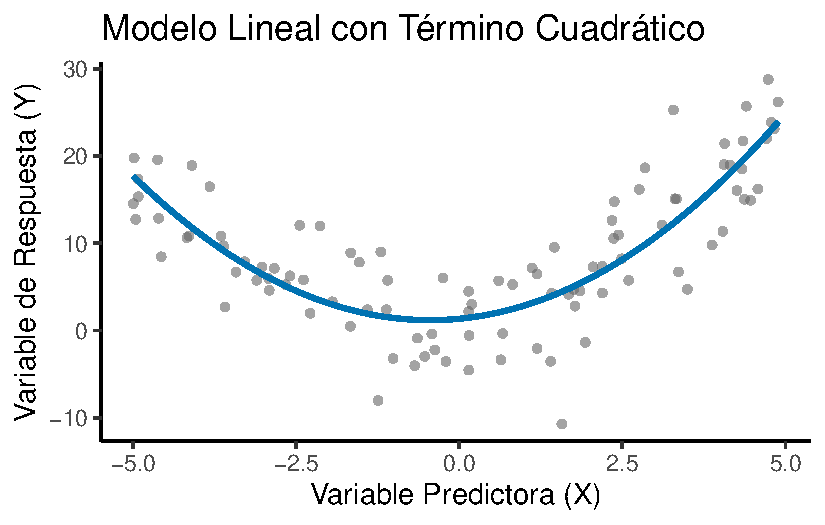
\includegraphics[keepaspectratio]{tema0_files/figure-pdf/fig-linear-params-1.pdf}}

}

\caption{\label{fig-linear-params}Ejemplo de un modelo lineal en los
parámetros que captura una relación no lineal (cuadrática) en los
datos.}

\end{figure}%

\end{tcolorbox}

\section{Un viaje preliminar por el universo de los modelos de
regresión}\label{sec-tipos-modelos}

La regresión lineal clásica, que será el objeto de estudio de los
primeros capítulos, es el punto de partida y la piedra angular sobre la
cual se erige una prolífica y fascinante gama de metodologías
estadísticas avanzadas. Este volumen se dedicará a desentrañar con rigor
las siguientes extensiones y especializaciones, que permiten al analista
abordar una variedad casi infinita de problemas.

\subsection{Modelos lineales (LMs)}\label{modelos-lineales-lms}

Constituyen el paradigma fundamental, el alfabeto sobre el que se
escribe el lenguaje del modelado estadístico. Son mucho más que una
simple técnica para ajustar una recta a una nube de puntos; son el
laboratorio donde se forjan y se comprenden los conceptos esenciales que
nos acompañarán durante todo nuestro viaje. Es aquí donde aprenderemos
a:

\begin{itemize}
\tightlist
\item
  \textbf{Estimar parámetros} e interpretar su significado en el
  contexto del problema.
\item
  \textbf{Cuantificar la incertidumbre} de nuestras estimaciones
  mediante errores estándar e intervalos de confianza.
\item
  \textbf{Realizar contrastes de hipótesis} para evaluar si la relación
  entre nuestras variables es estadísticamente significativa o fruto del
  azar.
\item
  \textbf{Diagnosticar la ``salud'' de un modelo}, examinando si los
  supuestos sobre los que se construye son razonables para nuestros
  datos.
\end{itemize}

En su forma más clásica, el modelo lineal asume que la variable de
respuesta (y, por consecuencia, el término de error aleatorio) sigue una
distribución Normal o Gaussiana. Esta asunción es la clave que
desbloquea todo el elegante aparato de la inferencia estadística,
permitiéndonos realizar pruebas exactas y derivar propiedades
matemáticas bien conocidas. Técnicas tan ubicuas en la ciencia como el
Análisis de la Varianza (ANOVA) o el Análisis de la Covarianza (ANCOVA)
no son más que casos particulares de la gran familia de los modelos
lineales, un hecho que unifica campos de la estadística que
históricamente se estudiaban por separado. Dominar los LMs es,
sencillamente, un requisito indispensable.

\subsection{Modelos lineales generalizados
(GLMs)}\label{modelos-lineales-generalizados-glms}

Si los LMs son el alfabeto, los GLMs son la gramática que nos permite
construir frases complejas y con significado en una variedad de
contextos mucho más amplia. Introducidos en el influyente y
verdaderamente revolucionario trabajo de (Nelder and Wedderburn 1972),
los GLMs representan un salto conceptual que expande de forma masiva el
universo de problemas que podemos abordar. Suponen una generalización
elegante que nos permite escapar de la ``tiranía'' de la distribución
Normal y modelar respuestas con una variedad mucho más amplia de
naturalezas y escalas.

Esta flexibilidad se logra mediante la combinación de dos ingeniosos
mecanismos que son el corazón de la teoría:

\begin{enumerate}
\def\labelenumi{\arabic{enumi}.}
\item
  \textbf{La familia exponencial de distribuciones}: Los GLMs no
  funcionan con cualquier distribución, sino con aquellas que pertenecen
  a una ``familia'' matemática con propiedades muy convenientes: la
  \textbf{familia exponencial}. Este ``club'' de distribuciones es muy
  selecto, pero incluye a miembros tan importantes como la Normal, la
  Poisson (para datos de conteo), la Binomial (para datos de
  proporciones o binarios), la Gamma (para datos continuos positivos y
  asimétricos) o la Binomial Negativa. Su estructura matemática común
  permite desarrollar una teoría unificada para la estimación de
  parámetros, lo que es un logro teórico de primer orden.
\item
  \textbf{La función de enlace (link function)}: Este es el verdadero
  golpe de genialidad. El predictor lineal de nuestro modelo,
  \(\boldsymbol{X\beta}\), puede tomar cualquier valor en la recta real,
  desde \(-\infty\) hasta \(+\infty\). Sin embargo, la media de nuestra
  variable de respuesta, \(E[Y] = \mu\), a menudo está restringida. Por
  ejemplo, una probabilidad (\(\mu\) en un modelo binomial) debe estar
  entre 0 y 1; un conteo (\(\mu\) en un modelo de Poisson) debe ser
  positivo. La función de enlace, \(g(\cdot)\), actúa como un
  \textbf{``traductor''} o un \textbf{``puente''} que conecta estos dos
  mundos. Transforma la media restringida de la respuesta para que pueda
  ser modelada por el predictor lineal no restringido. La relación
  fundamental es, por tanto, \(g(E[Y]) = g(\mu) = \boldsymbol{X\beta}\).
\end{enumerate}

\begin{itemize}
\tightlist
\item
  Para datos de \textbf{conteo} (Poisson), se usa un \textbf{enlace
  logarítmico} (\(g(\mu) = \log(\mu)\)). Esto garantiza que, al invertir
  la función para obtener la media
  (\(\mu = \exp(\boldsymbol{X\beta})\)), el resultado será siempre
  positivo, como debe ser un conteo.
\item
  Para datos \textbf{binarios} (Binomial), se usa un \textbf{enlace
  logit} (\(g(\mu) = \log(\frac{\mu}{1-\mu})\)). Esta función toma una
  probabilidad \(\mu\) en el rango (0, 1) y la proyecta sobre toda la
  recta real, permitiendo que sea modelada por \(\boldsymbol{X\beta}\).
\end{itemize}

Gracias a los GLMs, podemos usar el mismo marco conceptual de la
regresión lineal para modelar una gama de fenómenos increíblemente
diversa, desde predecir la cantidad de ciclistas en una ciudad (Poisson)
hasta la probabilidad de que un paciente responda a un tratamiento
(logística).

\subsection{Modelos de efectos mixtos (Mixed
Models)}\label{modelos-de-efectos-mixtos-mixed-models}

Su desarrollo responde a la necesidad crítica de analizar datos que
exhiben estructuras de dependencia o correlación, como agrupamientos,
anidamientos o jerarquías. En datos estándar, asumimos que las
observaciones son independientes, pero esta asunción se viola en casos
como: * \textbf{Medidas repetidas} sobre los mismos sujetos (ej: medir
la presión arterial de un paciente cada mes). * \textbf{Datos
longitudinales} (un tipo de medida repetida a lo largo del tiempo). *
\textbf{Datos agrupados} (ej: estudiantes anidados dentro de clases, que
a su vez están anidadas dentro de colegios). Estos modelos, detallados
en obras como la de (Pinheiro and Bates 2000), introducen explícitamente
una estructura de correlación en el término de error mediante la
incorporación de \textbf{efectos aleatorios}, que permiten capturar la
variabilidad entre los diferentes grupos o individuos, además de los
\textbf{efectos fijos} que representan a la población general.

\subsection{Modelos aditivos generalizados
(GAMs)}\label{modelos-aditivos-generalizados-gams}

Representan una extensión natural y altamente flexible de los GLMs que
relaja el supuesto de linealidad entre el predictor transformado y las
covariables. Los GAMs, cuya implementación moderna se debe en gran parte
al trabajo de (Wood 2017), permiten modelar estas relaciones mediante
\textbf{funciones suaves} no paramétricas (como \emph{splines}),
manteniendo al mismo tiempo la estructura aditiva del modelo. La forma
general es
\(g(\mu) = \alpha + f_1(x_1) + f_2(x_2) + \ldots + f_p(x_p)\), donde las
\(f_i(\cdot)\) son funciones suaves de los predictores estimadas a
partir de los datos. Esto permite capturar patrones no lineales
complejos sin necesidad de especificar una forma funcional paramétrica a
priori, logrando un equilibrio excepcional entre flexibilidad e
interpretabilidad.

\begin{tcolorbox}[enhanced jigsaw, leftrule=.75mm, breakable, colbacktitle=quarto-callout-note-color!10!white, bottomrule=.15mm, colframe=quarto-callout-note-color-frame, toprule=.15mm, colback=white, coltitle=black, bottomtitle=1mm, left=2mm, title=\textcolor{quarto-callout-note-color}{\faInfo}\hspace{0.5em}{R como lenguaje del modelado estadístico}, opacityback=0, arc=.35mm, opacitybacktitle=0.6, toptitle=1mm, titlerule=0mm, rightrule=.15mm]

Este compendio no es un texto puramente teórico. Fusiona intrínsecamente
la exposición de los conceptos con su aplicación computacional directa a
través del lenguaje y entorno estadístico \textbf{R}. R se ha
consolidado como el estándar de facto en la investigación estadística y
la ciencia de datos académica por su potencia, flexibilidad y el inmenso
ecosistema de paquetes contribuidos por la comunidad científica. Se
presupone en el lector una familiaridad operativa básica con R, y se
fomenta activamente el desarrollo de una fluidez progresiva mediante la
reproducción, modificación y experimentación con los numerosos ejemplos
y fragmentos de código presentados.

La capacidad de ejecutar análisis en R es fundamental para todo el ciclo
de vida del modelado:

\begin{itemize}
\tightlist
\item
  La \textbf{exploración de datos} y la visualización inicial.
\item
  La \textbf{estimación de parámetros} y el ajuste de los modelos.
\item
  El \textbf{diagnóstico riguroso} de la adecuación del modelo y la
  validación de sus supuestos.
\item
  La \textbf{producción de gráficos} y tablas de alta calidad para
  comunicar los resultados.
\end{itemize}

En R, las herramientas fundamentales para la regresión lineal
(\texttt{lm()}) y los modelos lineales generalizados (\texttt{glm()})
están incluidas en el paquete \textbf{\texttt{stats}}, que es uno de los
\textbf{paquetes base} y se carga automáticamente con cada sesión. Por
lo tanto, no necesitamos instalarlo ni cargarlo.

A lo largo del libro, extenderemos esta funcionalidad base con paquetes
especializados que sí requieren instalación y carga. Entre los más
importantes que usaremos se encuentran:

\begin{itemize}
\tightlist
\item
  \texttt{mgcv}: La implementación de referencia para GAMs, mantenida
  por su creador, Simon Wood, y citada en (Wood 2017).
\item
  \texttt{lme4} y \texttt{nlme}: Los dos paquetes fundamentales para el
  ajuste de modelos de efectos mixtos, desarrollados por los pioneros en
  el campo (Pinheiro and Bates 2000; Bates et al. 2015).
\item
  \texttt{rms}: Un paquete y una filosofía de trabajo para implementar
  estrategias de modelado de regresión robustas, como se detalla en la
  obra de (Harrell 2015).
\item
  \texttt{gamair}: Contiene numerosos conjuntos de datos que acompañan
  al libro de (Wood 2017), ideales para practicar con GAMs.
\end{itemize}

\end{tcolorbox}

\section{Una breve crónica del desarrollo de la
regresión}\label{sec-historia}

\subsection{Los orígenes: Galton y la ``regresión a la
mediocridad''}\label{los-oruxedgenes-galton-y-la-regresiuxf3n-a-la-mediocridad}

La gestación de la metodología de regresión se traza hasta las
investigaciones pioneras de Sir \textbf{Francis Galton}, un polímata de
la era victoriana. A finales del siglo XIX, estudiando la herencia de la
estatura, Galton recopiló datos de padres e hijos y notó un fenómeno
curioso: los padres muy altos tendían a tener hijos altos, pero, en
promedio, no tan altos como ellos. Análogamente, los padres muy bajos
tenían hijos bajos, pero no tan bajos como ellos. Acuñó el término
\textbf{``regresión a la mediocridad''} (hoy diríamos ``regresión a la
media'') para describir esta tendencia de las características de la
descendencia a ``regresar'' hacia la media de la población, en lugar de
perpetuar los extremos de los progenitores (Galton 1886).

\begin{tcolorbox}[enhanced jigsaw, leftrule=.75mm, breakable, colbacktitle=quarto-callout-tip-color!10!white, bottomrule=.15mm, colframe=quarto-callout-tip-color-frame, toprule=.15mm, colback=white, coltitle=black, bottomtitle=1mm, left=2mm, title=\textcolor{quarto-callout-tip-color}{\faLightbulb}\hspace{0.5em}{Estudios de Galton sobre estatura}, opacityback=0, arc=.35mm, opacitybacktitle=0.6, toptitle=1mm, titlerule=0mm, rightrule=.15mm]

\textbf{Datos recopilados}

\begin{itemize}
\tightlist
\item
  Galton recopiló datos sobre las estaturas de \textbf{928 hijos} y sus
  respectivos \textbf{padres}.
\item
  Las medidas fueron expresadas en pulgadas (1 pulgada = 2.54 cm).\\
\item
  En sus análisis, utilizó el promedio de las estaturas de ambos padres,
  conocido como \textbf{estatura media parental}, para compararlo con la
  estatura de los hijos.
\end{itemize}

\textbf{Principales hallazgos}

\begin{enumerate}
\def\labelenumi{\arabic{enumi}.}
\item
  \textbf{Relación lineal entre padres e hijos:}\\
  Galton observó que existe una relación positiva entre la estatura de
  los padres y la de los hijos. Los padres altos tienden a tener hijos
  altos, y los padres bajos tienden a tener hijos bajos. Esta relación
  puede modelarse con una línea recta, lo que inspiró la formulación de
  la regresión lineal.
\item
  \textbf{Regresión a la media:}

  \begin{itemize}
  \tightlist
  \item
    Aunque los hijos de padres altos son, en promedio, más altos que el
    promedio general de la población, también tienden a ser
    \textbf{menos altos que sus padres}.\\
  \item
    De manera similar, los hijos de padres bajos son más bajos que el
    promedio general, pero suelen ser \textbf{menos bajos que sus
    padres}.\\
  \item
    Este fenómeno, que Galton llamó ``regresión a la media'', ocurre
    porque las características extremas tienden a suavizarse en la
    siguiente generación debido a la influencia de múltiples factores
    genéticos y ambientales.
  \end{itemize}
\item
  \textbf{Ecuación de la recta de regresión:}\\
  Galton ajustó una recta para describir la relación entre la estatura
  media parental (\(X\)) y la estatura de los hijos (\(Y\)): \[
  Y = \beta_0 + \beta_1 X
  \] Donde:

  \begin{itemize}
  \tightlist
  \item
    \(\beta_0\): Intercepto, representa la estatura promedio de los
    hijos cuando la estatura parental es promedio.
  \item
    \(\beta_1\): Pendiente, indica cómo cambia la estatura de los hijos
    por cada unidad de cambio en la estatura media parental.
  \end{itemize}
\end{enumerate}

\textbf{Importancia en la Estadística}

\begin{enumerate}
\def\labelenumi{\arabic{enumi}.}
\item
  \textbf{Regresión lineal:}\\
  Este estudio introdujo el concepto de \textbf{recta de regresión}, que
  describe cómo varía la media de una variable dependiente en función de
  una variable independiente.
\item
  \textbf{Correlación:}\\
  Galton también estudió el grado de relación entre variables, precursor
  del concepto de \textbf{coeficiente de correlación} desarrollado
  posteriormente por Karl Pearson, un discípulo suyo.
\item
  \textbf{Regresión a la media:}\\
  El término y la idea detrás de ``regresión a la media'' surgieron de
  estos estudios y son hoy fundamentales en estadística y genética.
\end{enumerate}

\textbf{Ejemplo Gráfico}

Galton representó sus datos en gráficos de dispersión, mostrando cómo
los puntos (pares de estatura media parental y estatura de los hijos) se
agrupan alrededor de la recta de regresión, ilustrando la tendencia
general de la relación.

\begin{Shaded}
\begin{Highlighting}[]
\CommentTok{\# Cargar los paquetes necesarios}
\FunctionTok{library}\NormalTok{(ggplot2)}
\FunctionTok{library}\NormalTok{(HistData)}

\CommentTok{\# Cargar los datos de Galton}
\FunctionTok{data}\NormalTok{(}\StringTok{"GaltonFamilies"}\NormalTok{)}

\CommentTok{\# Crear el modelo de regresión lineal para obtener los coeficientes}
\NormalTok{modelo }\OtherTok{\textless{}{-}} \FunctionTok{lm}\NormalTok{(childHeight }\SpecialCharTok{\textasciitilde{}}\NormalTok{ midparentHeight, }\AttributeTok{data =}\NormalTok{ GaltonFamilies)}

\CommentTok{\# Crear la etiqueta para la ecuación de la recta de forma más limpia}
\CommentTok{\# Usamos sprintf() para un formato más controlado y legible}
\NormalTok{eq\_label }\OtherTok{\textless{}{-}} \FunctionTok{sprintf}\NormalTok{(}\StringTok{"y = \%.2f + \%.2f * x"}\NormalTok{, }\FunctionTok{coef}\NormalTok{(modelo)[}\DecValTok{1}\NormalTok{], }\FunctionTok{coef}\NormalTok{(modelo)[}\DecValTok{2}\NormalTok{])}

\CommentTok{\# {-}{-}{-} Gráfico Mejorado {-}{-}{-}}
\CommentTok{\# Usamos un tema más limpio y colores más suaves para una apariencia profesional.}
\CommentTok{\# geom\_jitter() es mejor que geom\_point() para estos datos, ya que evita la superposición de puntos.}
\FunctionTok{ggplot}\NormalTok{(GaltonFamilies, }\FunctionTok{aes}\NormalTok{(}\AttributeTok{x =}\NormalTok{ midparentHeight, }\AttributeTok{y =}\NormalTok{ childHeight)) }\SpecialCharTok{+}
  
  \CommentTok{\# 1. Puntos de datos: Usamos geom\_jitter para visualizar mejor los puntos superpuestos}
  \CommentTok{\#    y añadimos transparencia (alpha) para ver la densidad.}
  \FunctionTok{geom\_jitter}\NormalTok{(}\AttributeTok{alpha =} \FloatTok{0.3}\NormalTok{, }\AttributeTok{color =} \StringTok{"gray50"}\NormalTok{, }\AttributeTok{width =} \FloatTok{0.1}\NormalTok{, }\AttributeTok{height =} \FloatTok{0.1}\NormalTok{) }\SpecialCharTok{+}
  
  \CommentTok{\# 2. Línea de regresión: En un color azul profesional y más gruesa para que destaque.}
  \FunctionTok{geom\_smooth}\NormalTok{(}\AttributeTok{method =} \StringTok{"lm"}\NormalTok{, }\AttributeTok{se =} \ConstantTok{FALSE}\NormalTok{, }\AttributeTok{color =} \StringTok{"\#0072B2"}\NormalTok{, }\AttributeTok{size =} \FloatTok{1.2}\NormalTok{) }\SpecialCharTok{+}
  
  \CommentTok{\# 3. Anotación: Añadimos la ecuación de la recta de forma elegante,}
  \CommentTok{\#    usando el mismo color que la línea para crear cohesión visual.}
  \FunctionTok{annotate}\NormalTok{(}
    \StringTok{"text"}\NormalTok{,}
    \AttributeTok{x =} \DecValTok{66}\NormalTok{, }\AttributeTok{y =} \DecValTok{74}\NormalTok{, }\CommentTok{\# Posición ajustada para mejor visibilidad}
    \AttributeTok{label =}\NormalTok{ eq\_label,}
    \AttributeTok{color =} \StringTok{"\#0072B2"}\NormalTok{, }\CommentTok{\# Mismo color que la línea}
    \AttributeTok{size =} \FloatTok{4.5}\NormalTok{, }\CommentTok{\# Tamaño de la fuente}
    \AttributeTok{fontface =} \StringTok{"italic"} \CommentTok{\# Cursiva para la ecuación}
\NormalTok{  ) }\SpecialCharTok{+}
  
  \CommentTok{\# 4. Títulos y etiquetas: Mejorados para mayor claridad y contexto.}
  \CommentTok{\#    Añadimos un subtítulo y una fuente.}
  \FunctionTok{labs}\NormalTok{(}
    \AttributeTok{title =} \StringTok{"Regresión de la Estatura de Hijos vs. Padres"}\NormalTok{,}
    \AttributeTok{x =} \StringTok{"Promedio de Estatura de los Padres (pulgadas)"}\NormalTok{,}
    \AttributeTok{y =} \StringTok{"Estatura del Hijo/a (pulgadas)"}\NormalTok{,}
    \AttributeTok{caption =} \StringTok{"Fuente: Paquete HistData de R"}
\NormalTok{  ) }\SpecialCharTok{+}
  
  \CommentTok{\# 5. Tema: Usamos un tema limpio y profesional como base.}
  \FunctionTok{theme\_classic}\NormalTok{(}\AttributeTok{base\_size =} \DecValTok{14}\NormalTok{)}
\end{Highlighting}
\end{Shaded}

\begin{verbatim}
`geom_smooth()` using formula = 'y ~ x'
\end{verbatim}

\begin{figure}[H]

{\centering \pandocbounded{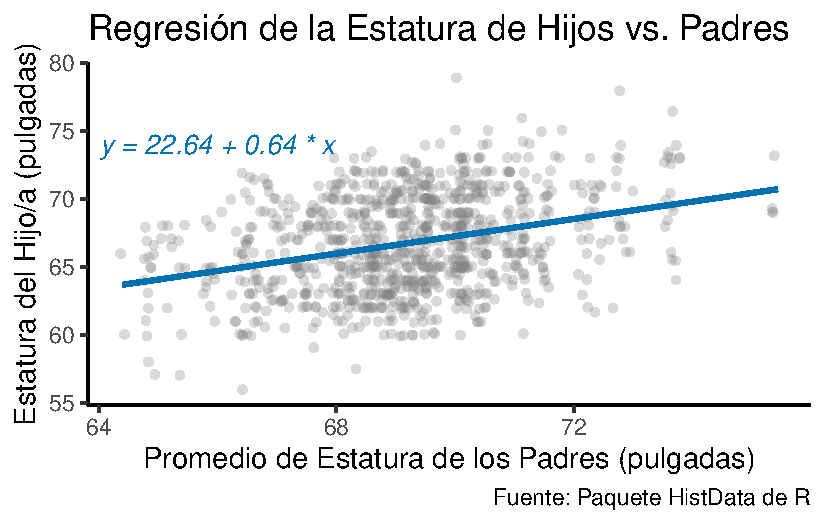
\includegraphics[keepaspectratio]{tema0_files/figure-pdf/galtonn-1.pdf}}

}

\caption{Datos históricos del estudio sobre la `regresión a la media'.}

\end{figure}%

\end{tcolorbox}

\subsection{La formalización matemática: Legendre y
Gauss}\label{la-formalizaciuxf3n-matemuxe1tica-legendre-y-gauss}

Aunque Galton sentó las bases conceptuales e introdujo el término, la
formalización matemática de la estimación de parámetros en modelos
lineales se atribuye a dos de los más grandes matemáticos de la
historia. \textbf{Adrien-Marie Legendre} publicó en 1805 el ``Método de
los mínimos cuadrados'' como un procedimiento numérico para ajustar
observaciones astronómicas. Pocos años después, \textbf{Carl Friedrich
Gauss} no solo publicó que había desarrollado el mismo método de forma
independiente años antes, sino que lo dotó de una profundidad teórica
mucho mayor, conectándolo con la teoría de la probabilidad y derivándolo
bajo el supuesto de errores distribuidos normalmente, convirtiéndolo en
la técnica fundamental para la estimación en modelos lineales que sigue
siendo hoy.

\subsection{El desarrollo moderno: la revolución de los
GLMs}\label{el-desarrollo-moderno-la-revoluciuxf3n-de-los-glms}

A lo largo del siglo XX, la regresión experimentó un desarrollo
explosivo. Sin embargo, el hito que probablemente más ha influido en la
práctica estadística moderna fue la publicación del artículo sobre
\textbf{Modelos Lineales Generalizados (GLMs)} por \textbf{John Nelder}
y \textbf{Robert Wedderburn} en 1972 (Nelder and Wedderburn 1972). Esta
obra seminal fue revolucionaria porque unificó bajo un mismo paraguas
conceptual y computacional diversas clases de modelos que hasta entonces
se trataban por separado: la regresión lineal para datos normales, la
regresión logística para datos binarios y la regresión de Poisson para
datos de conteo. Esto estimuló enormemente el desarrollo de software y
la aplicación del modelado estadístico a una nueva y vasta gama de
problemas.

\subsection{La evolución
contemporánea}\label{la-evoluciuxf3n-contemporuxe1nea}

Este legado continúa evolucionando a un ritmo vertiginoso, con la
inclusión de modelos jerárquicos y bayesianos, métodos no paramétricos y
de \emph{machine learning} como los árboles de regresión, y la
adaptación de la regresión al análisis de datos masivos (\emph{big
data}). La regresión ha evolucionado desde una observación sobre la
herencia biológica hasta convertirse en una de las herramientas más
versátiles y poderosas del arsenal analítico moderno.

\bookmarksetup{startatroot}

\chapter{El modelo de regresión lineal
simple}\label{sec-regresion-lineal-simple}

La regresión lineal constituye uno de los pilares fundamentales de la
modelización estadística. Es, a menudo, el primer y más importante
modelo predictivo que se aprende, no solo por su simplicidad e
interpretabilidad, sino porque los conceptos que exploraremos aquí son
la base sobre la que se construyen técnicas mucho más avanzadas, como el
\textbf{modelo de regresión lineal múltiple}, los \textbf{modelos
lineales generalizados (GLM)} o incluso conceptos utilizados en
algoritmos de \emph{machine learning} (Draper 1998; Kutner et al. 2005;
James et al. 2021).

En este capítulo, daremos el primer y más crucial paso en nuestro viaje
por el modelado predictivo: el estudio del \textbf{modelo de regresión
lineal simple}. Para ello, seguiremos el ciclo de vida completo de un
proyecto de modelado: comenzaremos con la exploración visual y
cuantitativa de los datos, formalizaremos después nuestras observaciones
mediante el lenguaje matemático del modelo y sus supuestos, aprenderemos
a estimar sus parámetros, realizaremos inferencias sobre ellos y,
finalmente, diagnosticaremos la validez de nuestro modelo (Fox and
Weisberg 2018; Harrell 2015).

La comprensión profunda que desarrollaremos aquí es esencial, ya que los
principios de estimación, inferencia y diagnóstico que aprenderemos son
directamente escalables al \textbf{modelo de regresión lineal múltiple},
que exploraremos en el siguiente capítulo.

\begin{tcolorbox}[enhanced jigsaw, leftrule=.75mm, breakable, colbacktitle=quarto-callout-important-color!10!white, bottomrule=.15mm, colframe=quarto-callout-important-color-frame, toprule=.15mm, colback=white, coltitle=black, bottomtitle=1mm, left=2mm, title=\textcolor{quarto-callout-important-color}{\faExclamation}\hspace{0.5em}{Objetivos de aprendizaje}, opacityback=0, arc=.35mm, opacitybacktitle=0.6, toptitle=1mm, titlerule=0mm, rightrule=.15mm]

Al finalizar este capítulo, serás capaz de:

\begin{enumerate}
\def\labelenumi{\arabic{enumi}.}
\tightlist
\item
  \textbf{Comprender y aplicar} el proceso de modelización estadística
  para un problema con una única variable predictora.
\item
  \textbf{Identificar y medir la correlación lineal} entre dos variables
  como paso previo al modelado.
\item
  \textbf{Describir la formulación matemática} del modelo de regresión
  lineal simple e interpretar el significado práctico de sus parámetros.
\item
  \textbf{Estimar los coeficientes} del modelo mediante el método de
  mínimos cuadrados ordinarios (MCO) y entender su derivación matemática
  y propiedades.
\item
  \textbf{Realizar inferencias sobre los parámetros} del modelo y
  evaluar su bondad de ajuste mediante el análisis de la varianza y el
  coeficiente de determinación R².
\item
  \textbf{Diagnosticar la adecuación del modelo}, evaluando visual y
  analíticamente si se cumplen los supuestos del modelo lineal.
\end{enumerate}

\end{tcolorbox}

\section{Exploración inicial: visualización y cuantificación de la
relación}\label{exploraciuxf3n-inicial-visualizaciuxf3n-y-cuantificaciuxf3n-de-la-relaciuxf3n}

Antes de sumergirnos en la teoría de la regresión, debemos hacer lo que
todo buen analista hace primero: \textbf{observar y cuantificar la
relación en los datos}. Este paso exploratorio es fundamental para
formular hipótesis y justificar la elección de un modelo lineal.

\subsection{Visualización: el gráfico de
dispersión}\label{visualizaciuxf3n-el-gruxe1fico-de-dispersiuxf3n}

La herramienta más potente para examinar la relación entre dos variables
continuas es el \textbf{gráfico de dispersión} (\emph{scatterplot}). Nos
permite intuir visualmente la \textbf{forma}, la \textbf{dirección} y la
\textbf{fuerza} de la relación. Una inspección visual es siempre el
punto de partida.

\subsection{Cuantificación de la asociación: covarianza y
correlación}\label{cuantificaciuxf3n-de-la-asociaciuxf3n-covarianza-y-correlaciuxf3n}

Una vez que la visualización sugiere una tendencia, necesitamos métricas
para cuantificarla.

\subsubsection{Covarianza}\label{covarianza}

La \textbf{covarianza} es una medida de la variabilidad conjunta de dos
variables aleatorias, \(X\) e \(Y\). Nos indica la dirección de la
relación lineal. La covarianza muestral, calculada a partir de nuestras
observaciones \((x_i, y_i)\), es:

\[
\text{Cov}(x, y) = s_{xy} = \frac{\sum_{i=1}^{n}(x_i - \bar{x})(y_i - \bar{y})}{n-1}
\]

El principal inconveniente de la covarianza es que su magnitud depende
de las unidades de las variables, lo que la hace difícil de interpretar.

\subsubsection{Coeficiente de correlación de
Pearson}\label{coeficiente-de-correlaciuxf3n-de-pearson}

Para solucionar el problema de la escala, estandarizamos la covarianza,
dividiéndola por el producto de las desviaciones típicas de cada
variable. El resultado es el \textbf{coeficiente de correlación de
Pearson (}\(r\)):

\[
r = r_{xy} = \frac{s_{xy}}{s_x s_y}
\]

Este coeficiente es \textbf{adimensional} y siempre varía entre
\textbf{-1 y 1}, lo que permite una interpretación universal de la
fuerza de la asociación \emph{lineal}.

\begin{tcolorbox}[enhanced jigsaw, leftrule=.75mm, breakable, colbacktitle=quarto-callout-tip-color!10!white, bottomrule=.15mm, colframe=quarto-callout-tip-color-frame, toprule=.15mm, colback=white, coltitle=black, bottomtitle=1mm, left=2mm, title=\textcolor{quarto-callout-tip-color}{\faLightbulb}\hspace{0.5em}{Ejemplo práctico: Horas de estudio vs.~Calificaciones}, opacityback=0, arc=.35mm, opacitybacktitle=0.6, toptitle=1mm, titlerule=0mm, rightrule=.15mm]

Vamos a plantear un problema que nos acompañará durante todo el
capítulo: queremos saber si el tiempo de estudio semanal influye en las
calificaciones finales.

\begin{Shaded}
\begin{Highlighting}[]
\FunctionTok{library}\NormalTok{(ggplot2)}
\FunctionTok{set.seed}\NormalTok{(}\DecValTok{123}\NormalTok{) }\CommentTok{\# Para reproducibilidad}

\CommentTok{\# Simulación de datos}
\NormalTok{datos }\OtherTok{\textless{}{-}} \FunctionTok{data.frame}\NormalTok{(}
  \AttributeTok{Tiempo\_Estudio =} \FunctionTok{round}\NormalTok{(}\FunctionTok{runif}\NormalTok{(}\DecValTok{100}\NormalTok{, }\AttributeTok{min =} \DecValTok{5}\NormalTok{, }\AttributeTok{max =} \DecValTok{40}\NormalTok{), }\DecValTok{1}\NormalTok{)}
\NormalTok{)}
\NormalTok{datos}\SpecialCharTok{$}\NormalTok{Calificaciones }\OtherTok{\textless{}{-}} \FunctionTok{round}\NormalTok{(}\DecValTok{5} \SpecialCharTok{+} \FloatTok{0.1} \SpecialCharTok{*}\NormalTok{ datos}\SpecialCharTok{$}\NormalTok{Tiempo\_Estudio }\SpecialCharTok{+} \FunctionTok{rnorm}\NormalTok{(}\DecValTok{100}\NormalTok{, }\AttributeTok{mean =} \DecValTok{0}\NormalTok{, }\AttributeTok{sd =} \FloatTok{0.5}\NormalTok{), }\DecValTok{2}\NormalTok{)}

\CommentTok{\# Visualización}
\FunctionTok{ggplot}\NormalTok{(datos, }\FunctionTok{aes}\NormalTok{(}\AttributeTok{x =}\NormalTok{ Tiempo\_Estudio, }\AttributeTok{y =}\NormalTok{ Calificaciones)) }\SpecialCharTok{+}
  \FunctionTok{geom\_point}\NormalTok{(}\AttributeTok{color =} \StringTok{"\#0072B2"}\NormalTok{, }\AttributeTok{alpha =} \FloatTok{0.7}\NormalTok{) }\SpecialCharTok{+}
  \FunctionTok{labs}\NormalTok{(}
    \AttributeTok{title =} \StringTok{"Relación entre Tiempo de Estudio y Calificaciones"}\NormalTok{,}
    \AttributeTok{x =} \StringTok{"Tiempo de Estudio (horas/semana)"}\NormalTok{,}
    \AttributeTok{y =} \StringTok{"Calificaciones (promedio)"}
\NormalTok{  ) }\SpecialCharTok{+}
  \FunctionTok{theme\_classic}\NormalTok{(}\AttributeTok{base\_size =} \DecValTok{14}\NormalTok{)}

\CommentTok{\# Cuantificación (los objetos se guardan para usarlos en el texto)}
\NormalTok{covarianza }\OtherTok{\textless{}{-}} \FunctionTok{cov}\NormalTok{(datos}\SpecialCharTok{$}\NormalTok{Tiempo\_Estudio, datos}\SpecialCharTok{$}\NormalTok{Calificaciones)}
\NormalTok{correlacion }\OtherTok{\textless{}{-}} \FunctionTok{cor}\NormalTok{(datos}\SpecialCharTok{$}\NormalTok{Tiempo\_Estudio, datos}\SpecialCharTok{$}\NormalTok{Calificaciones)}
\end{Highlighting}
\end{Shaded}

\begin{figure}[H]

\centering{

\pandocbounded{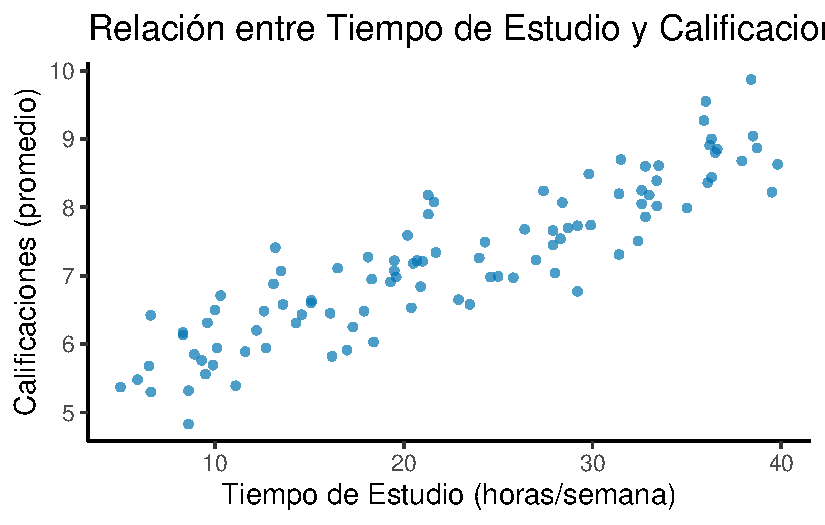
\includegraphics[keepaspectratio]{tema1_files/figure-pdf/fig-exploracion-inicial-full-1.pdf}}

}

\caption{\label{fig-exploracion-inicial-full}Relación entre tiempo de
estudio y calificaciones.}

\end{figure}%

El gráfico muestra una clara tendencia lineal positiva. La covarianza
toma un valor de 9.82, y el coeficiente de correlación de Pearson es de
0.9. Ambos valores confirman que la asociación lineal es, además de
positiva, muy fuerte. Esta evidencia visual y numérica nos da una base
sólida para proponer un modelo de regresión lineal.

\end{tcolorbox}

\begin{tcolorbox}[enhanced jigsaw, leftrule=.75mm, breakable, colbacktitle=quarto-callout-warning-color!10!white, bottomrule=.15mm, colframe=quarto-callout-warning-color-frame, toprule=.15mm, colback=white, coltitle=black, bottomtitle=1mm, left=2mm, title=\textcolor{quarto-callout-warning-color}{\faExclamationTriangle}\hspace{0.5em}{¡Correlación no implica causalidad!}, opacityback=0, arc=.35mm, opacitybacktitle=0.6, toptitle=1mm, titlerule=0mm, rightrule=.15mm]

El haber encontrado una fuerte correlación positiva entre el tiempo de
estudio y las calificaciones (0.9) no nos autoriza a concluir que
\emph{una cosa causa la otra}. La regresión lineal puede demostrar que
las variables se mueven juntas y nos permite predecir una a partir de la
otra, pero no explica el porqué de la relación.

Podría existir una tercera variable oculta (p.~ej., el interés del
alumno en la materia) que influya tanto en las horas de estudio como en
las calificaciones. Establecer causalidad requiere un diseño
experimental riguroso (asignando aleatoriamente a los estudiantes a
diferentes tiempos de estudio), no solo un análisis observacional.

\end{tcolorbox}

\section{Formulación teórica del
modelo}\label{formulaciuxf3n-teuxf3rica-del-modelo}

Una vez que la exploración sugiere una relación lineal, el siguiente
paso es formalizarla matemáticamente. Aquí es donde definimos la
estructura teórica del modelo y los supuestos bajo los cuales operará.

\subsection{El modelo poblacional y sus
componentes}\label{el-modelo-poblacional-y-sus-componentes}

El \textbf{modelo poblacional} postula que la relación verdadera entre
la variable respuesta \(Y\) y la predictora \(X\) sigue una línea recta,
aunque contaminada por cierta aleatoriedad. Para cualquier individuo
\(i\) de la población, esta relación se describe como:

\[
Y_i = \beta_0 + \beta_1 X_i + \varepsilon_i
\]

En esta ecuación, \(\beta_0\) y \(\beta_1\) son los \textbf{parámetros
poblacionales} (el intercepto y la pendiente verdaderos pero
desconocidos), y \(\varepsilon_i\) es el \textbf{error aleatorio}, un
componente fundamental que captura todas las fuentes de variabilidad que
el modelo no puede explicar por sí solo. Específicamente, este término
incluye:

\begin{itemize}
\tightlist
\item
  \textbf{Variables omitidas:} Factores que también afectan a las
  calificaciones (como la calidad del sueño, la motivación del
  estudiante o su conocimiento previo) y que no están en el modelo.
\item
  \textbf{Error de medida:} Pequeñas imprecisiones al medir las
  variables (p.~ej., un estudiante podría reportar 20 horas de estudio
  cuando en realidad fueron 19.5).
\item
  \textbf{Aleatoriedad inherente:} La variabilidad puramente estocástica
  o impredecible en el comportamiento humano.
\end{itemize}

Como nunca observamos la población entera, nuestro trabajo consiste en
usar una muestra para estimar el \textbf{modelo muestral}:

\[
\hat{y}_i = \hat{\beta}_0 + \hat{\beta}_1 x_i
\]

Aquí, los ``gorros'' (\(\hat{\cdot}\)) denotan \textbf{estimaciones}
calculadas a partir de la muestra. La diferencia entre el valor real y
el predicho, \(e_i = y_i - \hat{y}_i\), se conoce como \textbf{residuo}.

\subsection{Los supuestos del modelo lineal clásico
(Gauss-Markov)}\label{los-supuestos-del-modelo-lineal-cluxe1sico-gauss-markov}

Para que el puente entre nuestro modelo muestral y la realidad
poblacional sea sólido, debemos asumir que los errores teóricos
\(\varepsilon_i\) se comportan de una manera predecible y ordenada.
Estos supuestos, conocidos como condiciones de Gauss-Markov (Kutner et
al. 2005; Weisberg 2005), son fundamentales para las propiedades óptimas
de los estimadores de mínimos cuadrados.

\begin{enumerate}
\def\labelenumi{\arabic{enumi}.}
\tightlist
\item
  \textbf{Linealidad}: La relación entre \(X\) y el valor esperado de
  \(Y\) es, en promedio, una línea recta:
  \(E[Y_i | X_i] = \beta_0 + \beta_1 X_i\).
\item
  \textbf{Independencia de los errores}: El error de una observación no
  está correlacionado con el error de ninguna otra:
  \(\text{Cov}(\varepsilon_i, \varepsilon_j) = 0\) para \(i \neq j\).
\item
  \textbf{Homocedasticidad}: La varianza del error es constante
  (\(\sigma^2\)) para todos los valores de \(X\):
  \(Var(\varepsilon_i | X_i) = \sigma^2\). Esto significa que la
  dispersión de los datos alrededor de la línea de regresión es la misma
  a lo largo de todos los valores de la variable predictora. La
  violación de este supuesto se conoce como \textbf{heterocedasticidad},
  donde la dispersión de los errores cambia (p.~ej., aumenta a medida
  que \(X\) crece).
\end{enumerate}

Cuando el objetivo no es sólo estimar la recta, sino inferir con ella,
entonces se asume una hipótesis más: la normalidad de la variable
respuesta, o lo que es lo mismo, del error aleatorio:

\begin{enumerate}
\def\labelenumi{\arabic{enumi}.}
\setcounter{enumi}{3}
\tightlist
\item
  \textbf{Normalidad de los errores}: Para la inferencia, se asume que
  los errores siguen una distribución Normal con media cero y varianza
  \(\sigma^2\): \(\varepsilon_i \sim N(0, \sigma^2)\).
\end{enumerate}

Estos supuestos son esenciales para garantizar la validez de las
estimaciones y conclusiones derivadas del modelo.

\section{Estimación de los
parámetros}\label{estimaciuxf3n-de-los-paruxe1metros}

Necesitamos un método para encontrar la ``mejor'' recta de ajuste. El
\textbf{Método de Mínimos Cuadrados Ordinarios (MCO/OLS)} nos
proporciona este criterio.

\subsection{El criterio de mínimos
cuadrados}\label{el-criterio-de-muxednimos-cuadrados}

MCO busca la recta que minimice la \textbf{Suma de los Cuadrados del
Error (SSE)}, es decir, la suma de las distancias verticales al cuadrado
entre los puntos observados y la recta de regresión:

\[
\text{SSE}(\beta_0, \beta_1) = \sum_{i=1}^{n} e_i^2 = \sum_{i=1}^{n} (y_i-\hat{y})^2 = \sum_{i=1}^{n} (y_i - (\beta_0 + \beta_1 x_i))^2
\]

\subsection{Derivación matemática de los
estimadores}\label{derivaciuxf3n-matemuxe1tica-de-los-estimadores}

Para encontrar los valores de \(\beta_0\) y \(\beta_1\) que minimizan
esta función, recurrimos al cálculo. Tratamos la SSE como una función de
dos variables y calculamos sus derivadas parciales, igualándolas a cero
para encontrar el mínimo.

\[
\frac{\partial \text{SSE}}{\partial \beta_0} = -2 \sum_{i=1}^{n} (y_i - \beta_0 - \beta_1 x_i) = 0
\]

\[
\frac{\partial \text{SSE}}{\partial \beta_1} = -2 \sum_{i=1}^{n} x_i (y_i - \beta_0 - \beta_1 x_i) = 0
\]

La resolución de este sistema de dos ecuaciones (conocidas como las
\textbf{ecuaciones normales}) nos proporciona las fórmulas para los
estimadores de MCO:

\[
\hat{\beta}_1 = \frac{\sum_{i=1}^{n}(x_i - \bar{x})(y_i - \bar{y})}{\sum_{i=1}^{n}(x_i - \bar{x})^2} = \frac{s_{xy}}{s_{xx}}
\] \[ \hat{\beta}_0 = \bar{y} - \hat{\beta}_1 \bar{x}
\]

\subsubsection{Interpretación práctica de los
coeficientes}\label{interpretaciuxf3n-pruxe1ctica-de-los-coeficientes}

Una vez estimados, los coeficientes tienen una interpretación muy
concreta y útil:

\begin{itemize}
\item
  \textbf{Pendiente} (\(\hat{\beta}_1\)): Representa el cambio promedio
  estimado en la variable respuesta \(Y\) por cada \textbf{aumento de
  una unidad} en la variable predictora \(X\). En nuestro ejemplo, sería
  el número de puntos que se espera que aumente la calificación final
  por cada hora adicional de estudio semanal.
\item
  \textbf{Intercepto} (\(\hat{\beta}_0\)): Es el valor promedio estimado
  de la variable respuesta \(Y\) cuando la variable predictora \(X\) es
  igual a cero. La interpretación del intercepto solo tiene sentido
  práctico si \(X=0\) es un valor plausible y se encuentra dentro del
  rango de nuestros datos. De lo contrario (como en nuestro ejemplo,
  donde nadie estudia 0 horas), a menudo se considera simplemente un
  ancla matemática para la recta de regresión.
\end{itemize}

\begin{tcolorbox}[enhanced jigsaw, leftrule=.75mm, breakable, colbacktitle=quarto-callout-note-color!10!white, bottomrule=.15mm, colframe=quarto-callout-note-color-frame, toprule=.15mm, colback=white, coltitle=black, bottomtitle=1mm, left=2mm, title=\textcolor{quarto-callout-note-color}{\faInfo}\hspace{0.5em}{Minimización de SSE}, opacityback=0, arc=.35mm, opacitybacktitle=0.6, toptitle=1mm, titlerule=0mm, rightrule=.15mm]

La obtención de los estimadores de mínimos cuadrados para la regresión
lineal simple se basa en minimizar la suma de los cuadrados de los
residuos (\(SSE\)). Este método, desarrollado por Legendre y Gauss a
principios del siglo XIX (Galton 1886; Weisberg 2005), es fundamental en
la estadística moderna. Aquí está el proceso paso a paso:

Para minimizar \(SSE\), derivamos parcialmente con respecto a
\(\beta_0\) y \(\beta_1\) y resolvemos el sistema de ecuaciones.

\begin{enumerate}
\def\labelenumi{\arabic{enumi}.}
\tightlist
\item
  \textbf{Primera derivada con respecto a} \(\beta_0\):
\end{enumerate}

\[
    \frac{\partial SSE}{\partial \beta_0} = -2\sum_{i=1}^n
    \left(y_i - (\beta_0 + \beta_1 x_i)\right).
  \]

\begin{verbatim}
Igualando a cero: 
\end{verbatim}

\[ 
    \sum_{i=1}^n \left(y_i - \beta_0 - \beta_1
    x_i\right) = 0. 
  \]

\begin{verbatim}
Reordenando: 
\end{verbatim}

\[
    n\beta_0 + \beta_1 \sum_{i=1}^n x_i = \sum_{i=1}^n y_i. \tag{1}
  \]

\begin{enumerate}
\def\labelenumi{\arabic{enumi}.}
\setcounter{enumi}{1}
\tightlist
\item
  \textbf{Primera derivada con respecto a} \(\beta_1\):
\end{enumerate}

\[
    \frac{\partial SSE}{\partial \beta_1} = -2\sum_{i=1}^n x_i
    \left(y_i - (\beta_0 + \beta_1 x_i)\right).
    \]

\begin{verbatim}
Igualando a cero: 
\end{verbatim}

\[ 
    \sum_{i=1}^n x_i \left(y_i - \beta_0 -
    \beta_1 x_i\right) = 0. 
   \]

\begin{verbatim}
Reordenando: 
\end{verbatim}

\[
    \beta_0 \sum_{i=1}^n x_i + \beta_1 \sum_{i=1}^n x_i^2 = \sum_{i=1}^n x_i y_i. \tag{2}
   \]

\textbf{Resolución del Sistema de Ecuaciones}

El sistema está dado por las ecuaciones (1) y (2):

\begin{enumerate}
\def\labelenumi{\arabic{enumi}.}
\tightlist
\item
  \(n\beta_0 + \beta_1 \sum_{i=1}^n x_i = \sum_{i=1}^n y_i.\)\\
\item
  \(\beta_0 \sum_{i=1}^n x_i + \beta_1 \sum_{i=1}^n x_i^2 = \sum_{i=1}^n x_i y_i.\)
\end{enumerate}

Resolviendo para \(\beta_0\) y \(\beta_1\):

\begin{enumerate}
\def\labelenumi{\arabic{enumi}.}
\item
  De la primera ecuación, despejamos \(\beta_0\):\\
  \[
  \beta_0 = \frac{\sum_{i=1}^n y_i - \beta_1 \sum_{i=1}^n x_i}{n}. \tag{3}
  \]
\item
  Sustituimos \(\beta_0\) en la segunda ecuación:\\
  \[
  \frac{\sum_{i=1}^n y_i - \beta_1 \sum_{i=1}^n x_i}{n} \sum_{i=1}^n x_i + \beta_1 \sum_{i=1}^n x_i^2 = \sum_{i=1}^n x_i y_i.
  \]

  Simplificando:\\
  \[
  \beta_1 \left(\sum_{i=1}^n x_i^2 - \frac{(\sum_{i=1}^n x_i)^2}{n}\right) = \sum_{i=1}^n x_i y_i - \frac{\sum_{i=1}^n x_i \sum_{i=1}^n y_i}{n}.
  \]
\item
  Expresamos \(\beta_1\):\\
  \[
  \beta_1 = \frac{\sum_{i=1}^n x_i y_i - \frac{\sum_{i=1}^n x_i \sum_{i=1}^n y_i}{n}}{\sum_{i=1}^n x_i^2 - \frac{(\sum_{i=1}^n x_i)^2}{n}}.
  \] Esta es la fórmula para \(\beta_1\), que puede reescribirse como:\\
  \[
  \beta_1 = \frac{\text{Cov}(x, y)}{\text{Var}(x)},
  \] donde \(\text{Cov}(x, y)\) y \(\text{Var}(x)\) son la covarianza y
  la varianza muestral de \(x\) y \(y\).
\item
  Finalmente, sustituimos \(\beta_1\) en la ecuación (3) para obtener
  \(\beta_0\):\\
  \[
  \beta_0 = \bar{y} - \beta_1 \bar{x},
  \] donde \(\bar{x}\) y \(\bar{y}\) son las medias de \(x\) y \(y\).
\end{enumerate}

\end{tcolorbox}

Bajo los supuestos del modelo, el \textbf{Teorema de Gauss-Markov}
demuestra que estos estimadores son los \textbf{Mejores Estimadores
Lineales Insesgados (MELI / BLUE)}.

\section{Inferencia y bondad de
ajuste}\label{inferencia-y-bondad-de-ajuste}

Una vez hemos estimado los parámetros del modelo, nuestro trabajo apenas
ha comenzado. Ahora debemos pasar de la descripción a la inferencia.
Necesitamos un conjunto de herramientas que nos permitan responder a
preguntas cruciales: ¿Son nuestros coeficientes estimados,
\(\hat{\beta}_0\) y \(\hat{\beta}_1\), meras casualidades de nuestra
muestra o reflejan una relación real en la población? ¿Qué tan bueno es
nuestro modelo para explicar la variabilidad de la variable respuesta?
Esta sección se dedica a responder estas preguntas.

\subsection{Propiedades de los estimadores de
MCO}\label{propiedades-de-los-estimadores-de-mco}

Antes de realizar inferencias, es fundamental entender las propiedades
teóricas de los estimadores que hemos calculado.

\begin{itemize}
\item
  \textbf{Insesgadez}: Los estimadores de MCO son insesgados. Esto
  significa que si pudiéramos repetir nuestro muestreo muchísimas veces
  y calcular los estimadores en cada muestra, el promedio de todas
  nuestras estimaciones de \(\hat{\beta}_0\) y \(\hat{\beta}_1\)
  convergería a los verdaderos valores poblacionales \(\beta_0\) y
  \(\beta_1\). Matemáticamente: \[
    E[\hat{\beta}_0] = \beta_0 \quad \text{y} \quad E[\hat{\beta}_1] = \beta_1
    \]
\item
  \textbf{Varianza de los estimadores}: Las fórmulas para la varianza de
  nuestros estimadores cuantifican su precisión. Una varianza pequeña
  implica que el estimador es más estable a través de diferentes
  muestras. \[
    Var(\hat{\beta}_1) = \frac{\sigma^2}{\sum_{i=1}^{n}(x_i - \bar{x})^2} = \frac{\sigma^2}{S_{xx}}
    \] \[
    Var(\hat{\beta}_0) = \sigma^2 \left[ \frac{1}{n} + \frac{\bar{x}^2}{S_{xx}} \right]
    \] Donde \(\sigma^2\) es la varianza (desconocida) del término de
  error \(\varepsilon\).
\item
  \textbf{Teorema de Gauss-Markov}: Este es uno de los resultados más
  importantes de la teoría de la regresión. Establece que, bajo los
  supuestos de linealidad, independencia y homocedasticidad (no se
  requiere normalidad), los estimadores de MCO son los \textbf{Mejores
  Estimadores Lineales Insesgados} (MELI, o BLUE en inglés). Esto
  significa que, de entre toda la clase de estimadores que son lineales
  e insesgados, los de MCO son los que tienen la menor varianza posible.
\end{itemize}

\begin{tcolorbox}[enhanced jigsaw, leftrule=.75mm, breakable, colbacktitle=quarto-callout-note-color!10!white, bottomrule=.15mm, colframe=quarto-callout-note-color-frame, toprule=.15mm, colback=white, coltitle=black, bottomtitle=1mm, left=2mm, title=\textcolor{quarto-callout-note-color}{\faInfo}\hspace{0.5em}{Propiedades adicionales para las predicciones y para los residuos}, opacityback=0, arc=.35mm, opacitybacktitle=0.6, toptitle=1mm, titlerule=0mm, rightrule=.15mm]

\begin{itemize}
\item
  La suma de los residuos es cero: \[
    \sum_{i=1}^n e_i=\sum_{i=1}^n(y_i-\hat{y_i})=0
    \]
\item
  La suma de los valores observados es igual a la suma de los valores
  ajustados: \[
    \sum_{i=1}^n y_i=\sum_{i=1}^n \hat{y_i}
    \]
\item
  La suma de los residuos ponderados por los regresores es cero: \[
    \sum_{i=1}^n x_ie_i=0
    \]
\item
  La suma de los residuos ponderados por las predicciones es cero: \[
    \sum_{i=1}^n \hat{y_i}e_i=0
    \]
\item
  La recta de regresión contiene el punto
  \((\bar{x},\bar{y})\):\[\hat{\beta_0} + \hat{\beta_1}\bar{x} = \bar{y}\]
\end{itemize}

\end{tcolorbox}

\begin{tcolorbox}[enhanced jigsaw, leftrule=.75mm, breakable, colbacktitle=quarto-callout-tip-color!10!white, bottomrule=.15mm, colframe=quarto-callout-tip-color-frame, toprule=.15mm, colback=white, coltitle=black, bottomtitle=1mm, left=2mm, title=\textcolor{quarto-callout-tip-color}{\faLightbulb}\hspace{0.5em}{Ejemplo}, opacityback=0, arc=.35mm, opacitybacktitle=0.6, toptitle=1mm, titlerule=0mm, rightrule=.15mm]

Para los datos de calificaciones y tiempo de estudio, estos son los
estimadores de los parámetros del modelo de regresión:

\begin{Shaded}
\begin{Highlighting}[]
\CommentTok{\# 1. Ajustamos el modelo lineal}
\NormalTok{modelo\_estudio }\OtherTok{\textless{}{-}} \FunctionTok{lm}\NormalTok{(Calificaciones }\SpecialCharTok{\textasciitilde{}}\NormalTok{ Tiempo\_Estudio, }\AttributeTok{data =}\NormalTok{ datos)}

\CommentTok{\# 2. Obtenemos el resumen completo del modelo}
\FunctionTok{summary}\NormalTok{(modelo\_estudio)}
\end{Highlighting}
\end{Shaded}

\begin{verbatim}

Call:
lm(formula = Calificaciones ~ Tiempo_Estudio, data = datos)

Residuals:
     Min       1Q   Median       3Q      Max 
-1.11465 -0.30262 -0.00942  0.29509  1.10533 

Coefficients:
               Estimate Std. Error t value Pr(>|t|)    
(Intercept)     5.00118    0.11977   41.76   <2e-16 ***
Tiempo_Estudio  0.09875    0.00488   20.23   <2e-16 ***
---
Signif. codes:  0 '***' 0.001 '**' 0.01 '*' 0.05 '.' 0.1 ' ' 1

Residual standard error: 0.4842 on 98 degrees of freedom
Multiple R-squared:  0.8069,    Adjusted R-squared:  0.8049 
F-statistic: 409.5 on 1 and 98 DF,  p-value: < 2.2e-16
\end{verbatim}

\end{tcolorbox}

\subsection{Estimación de la varianza del
error}\label{estimaciuxf3n-de-la-varianza-del-error}

Las fórmulas de la varianza de los estimadores dependen de \(\sigma^2\),
la varianza del error poblacional, que es desconocida. Por lo tanto,
necesitamos estimarla a partir de nuestros datos. Un estimador insesgado
de \(\sigma^2\) es la \textbf{Media Cuadrática del Error (MSE)}:

\[
\hat{\sigma}^2 = \text{MSE} = \frac{\text{SSE}}{n-2} = \frac{\sum_{i=1}^{n}(y_i - \hat{y}_i)^2}{n-2}
\]

Dividimos por \(n-2\), los \textbf{grados de libertad del error}, porque
hemos ``gastado'' dos grados de libertad de nuestros datos para estimar
los dos parámetros, \(\beta_0\) y \(\beta_1\). La raíz cuadrada de la
MSE, \(\hat{\sigma}\), se conoce como el \textbf{error estándar de los
residuos} y es una medida de la dispersión promedio de los puntos
alrededor de la recta de regresión.

\subsubsection{El error estándar de los residuos y el
RMSE}\label{el-error-estuxe1ndar-de-los-residuos-y-el-rmse}

La raíz cuadrada de la MSE, \(\hat{\sigma}\), se conoce formalmente como
el \textbf{error estándar de los residuos} (\emph{Residual Standard
Error}). Este valor es nuestra estimación de la desviación estándar del
error poblacional, \(\sigma\), y es una medida de la dispersión promedio
de los puntos alrededor de la recta de regresión.

\[
\hat{\sigma} = \sqrt{\text{MSE}}
\]

En el campo del modelado predictivo y el \emph{machine learning}, esta
misma cantidad se conoce como la \textbf{Raíz del Error Cuadrático
Medio} o \textbf{RMSE} (\emph{Root Mean Squared Error}). Aunque la
fórmula es idéntica, la interpretación del RMSE se centra en la
\textbf{evaluación del rendimiento predictivo} del modelo. El RMSE nos
dice, en promedio, cuál es la magnitud del error de predicción de
nuestro modelo, y tiene la ventaja de estar en las \textbf{mismas
unidades} que la variable respuesta \(Y\). Por ejemplo, si estamos
prediciendo precios de viviendas en euros, un RMSE de 5000 significa que
nuestras predicciones se desvían, en promedio, unos 5000 € de los
precios reales.

\subsection{Análisis de la Varianza (ANOVA) para la significancia de la
regresión}\label{anuxe1lisis-de-la-varianza-anova-para-la-significancia-de-la-regresiuxf3n}

Una vez hemos estimado los coeficientes, necesitamos una prueba formal
para determinar si el modelo en su conjunto es útil. Es decir, ¿la
variable predictora \(X\) explica una porción de la variabilidad de la
variable respuesta \(Y\) que sea estadísticamente significativa, o la
relación que observamos podría deberse simplemente al azar? El
\textbf{Análisis de la Varianza (ANOVA)} nos proporciona la herramienta
para responder a esta pregunta a través del \textbf{contraste F de
significancia global}.

Las hipótesis de este contraste son:

\begin{itemize}
\tightlist
\item
  \(H_0: \beta_1 = 0\): La hipótesis nula postula que no existe una
  relación lineal entre \(X\) e \(Y\). El modelo no tiene poder
  explicativo y no es mejor que usar simplemente la media, \(\bar{y}\),
  como predicción para cualquier valor de \(x\).
\item
  \(H_1: \beta_1 \neq 0\): La hipótesis alternativa sostiene que sí
  existe una relación lineal significativa.
\end{itemize}

\begin{tcolorbox}[enhanced jigsaw, leftrule=.75mm, breakable, colbacktitle=quarto-callout-caution-color!10!white, bottomrule=.15mm, colframe=quarto-callout-caution-color-frame, toprule=.15mm, colback=white, coltitle=black, bottomtitle=1mm, left=2mm, title=\textcolor{quarto-callout-caution-color}{\faFire}\hspace{0.5em}{Repaso}, opacityback=0, arc=.35mm, opacitybacktitle=0.6, toptitle=1mm, titlerule=0mm, rightrule=.15mm]

Es conveniente repasar el tema de \emph{Análisis de la Varianza}
estudiado en la asignatura de Inferencia, ya que los conceptos son
directamente aplicables aquí.

\end{tcolorbox}

La idea fundamental del ANOVA es comparar la variabilidad que nuestro
modelo \emph{explica} con la variabilidad que \emph{no puede explicar}
(el error residual). Para ello, se descompone la variabilidad total de
nuestras observaciones (\(y_i\)) en dos partes ortogonales.

\begin{enumerate}
\def\labelenumi{\arabic{enumi}.}
\item
  La \textbf{Suma Total de Cuadrados (SST)} mide la variabilidad total
  de los datos alrededor de su media. Es nuestra referencia base de la
  dispersión total que hay que explicar. \[
  \text{SST} = \sum_{i=1}^{n} (y_i - \bar{y})^2
  \]
\item
  Esta variabilidad se descompone en:

  \begin{itemize}
  \tightlist
  \item
    \textbf{Suma de Cuadrados de la Regresión (SSR)}: Mide la parte de
    la variabilidad total que es explicada por nuestro modelo.
    Cuantifica cuánto se desvían las predicciones del modelo
    (\(\hat{y}_i\)) de la media general (\(\bar{y}\)). \[
      \text{SSR} = \sum_{i=1}^{n} (\hat{y}_i - \bar{y})^2
      \]
  \item
    \textbf{Suma de Cuadrados del Error (SSE)}: Mide la variabilidad
    residual, es decir, la parte que el modelo no puede capturar.
    Cuantifica la dispersión de los puntos reales (\(y_i\)) alrededor de
    la recta de regresión (\(\hat{y}_i\)). \[
      \text{SSE} = \sum_{i=1}^{n} (y_i - \hat{y}_i)^2
      \]
  \end{itemize}
\end{enumerate}

La descomposición fundamental de la varianza es, por tanto:
\(\text{SST} = \text{SSR} + \text{SSE}\).

Para poder comparar estas sumas de cuadrados de forma justa, las
estandarizamos dividiéndolas por sus respectivos \textbf{grados de
libertad}, obteniendo así las \textbf{Medias Cuadráticas} (MS):

\[
\text{MSR} = \frac{\text{SSR}}{1} \quad \quad \quad \text{MSE} = \frac{\text{SSE}}{n-2}
\]

Finalmente, el \textbf{estadístico F} se construye como el cociente
entre la variabilidad explicada por el modelo y la variabilidad no
explicada:

\[
F = \frac{\text{MSR}}{\text{MSE}}
\]

Intuitivamente, el estadístico F actúa como una \textbf{ratio de señal a
ruido}. La MSR (la ``señal'') representa la variabilidad que nuestro
modelo captura sistemáticamente, mientras que la MSE (el ``ruido'')
representa la variabilidad aleatoria o residual. Un valor de F grande
nos dice que la señal es mucho más fuerte que el ruido, lo que apoya la
hipótesis de que la relación que hemos modelado es real y no fruto del
azar.

Toda esta información se organiza de forma estándar en la \textbf{tabla
ANOVA}:

\begin{longtable}[]{@{}lllll@{}}
\toprule\noalign{}
Fuente & \(df\) & \(SS\) & \(MS = SS/df\) & Estadístico \(F\) \\
\midrule\noalign{}
\endhead
\bottomrule\noalign{}
\endlastfoot
Regresión & 1 & \(SSR\) & \(MSR\) & \(F = MSR/MSE\) \\
Error & \(n-2\) & \(SSE\) & \(MSE\) & \\
Total & \(n-1\) & \(SST\) & & \\
\end{longtable}

Bajo la hipótesis nula (\(H_0: \beta_1 = 0\)), el estadístico \(F\)
sigue una distribución \(F\) con 1 y \(n-2\) grados de libertad. Si el
p-valor asociado a nuestro estadístico F es suficientemente pequeño
(\(p < \alpha\)), rechazamos \(H_0\) y concluimos que nuestro modelo
tiene un poder explicativo estadísticamente significativo.

\subsection{Bondad del ajuste: coeficiente de
determinación}\label{bondad-del-ajuste-coeficiente-de-determinaciuxf3n}

El coeficiente de determinación (\(R^2\)) es una medida clave que
cuantifica qué proporción de la variabilidad total observada en la
muestra (\(y_i\)) es explicada por la relación lineal con \(X\) a través
del modelo. Su fórmula se deriva de la descomposición de la varianza:

\[
R^2 = \frac{\text{SSR}}{\text{SST}} = 1 - \frac{\text{SSE}}{\text{SST}}
\]

Donde las sumas de cuadrados se calculan a partir de los datos
muestrales:

\begin{itemize}
\tightlist
\item
  \(\text{SST} = \sum_{i=1}^n (y_i - \bar{y})^2\): Suma Total de
  Cuadrados, mide la variabilidad total de las observaciones.
\item
  \(\text{SSR} = \sum_{i=1}^n (\hat{y}_i - \bar{y})^2\): Suma de
  Cuadrados de la Regresión, mide la variabilidad explicada por el
  modelo.
\item
  \(\text{SSE} = \sum_{i=1}^n (y_i - \hat{y}_i)^2\): Suma de Cuadrados
  del Error, mide la variabilidad no explicada (residual).
\end{itemize}

Un \(R^2\) cercano a 1 indica que el modelo ajusta bien los datos,
mientras que un \(R^2\) cercano a 0 indica un ajuste pobre.

\begin{tcolorbox}[enhanced jigsaw, leftrule=.75mm, breakable, colbacktitle=quarto-callout-note-color!10!white, bottomrule=.15mm, colframe=quarto-callout-note-color-frame, toprule=.15mm, colback=white, coltitle=black, bottomtitle=1mm, left=2mm, title=\textcolor{quarto-callout-note-color}{\faInfo}\hspace{0.5em}{Relación entre R² y el coeficiente de correlación}, opacityback=0, arc=.35mm, opacitybacktitle=0.6, toptitle=1mm, titlerule=0mm, rightrule=.15mm]

En el caso específico del modelo de regresión lineal simple, existe una
relación directa y simple: el coeficiente de determinación \(R^2\) es
literalmente el cuadrado del coeficiente de correlación de Pearson
(\(r\)) entre \(X\) e \(Y\).

\[ R^2 = (r_{xy})^2 \]

Esto refuerza la idea de que ambos miden la fuerza de la asociación
\emph{lineal}, aunque \(R^2\) lo hace desde la perspectiva de la
varianza explicada por el modelo.

\end{tcolorbox}

\begin{tcolorbox}[enhanced jigsaw, leftrule=.75mm, breakable, colbacktitle=quarto-callout-caution-color!10!white, bottomrule=.15mm, colframe=quarto-callout-caution-color-frame, toprule=.15mm, colback=white, coltitle=black, bottomtitle=1mm, left=2mm, title=\textcolor{quarto-callout-caution-color}{\faFire}\hspace{0.5em}{Interpretación de R²}, opacityback=0, arc=.35mm, opacitybacktitle=0.6, toptitle=1mm, titlerule=0mm, rightrule=.15mm]

El coeficiente de determinación, \(R^2\), es una métrica muy popular,
pero su interpretación requiere cautela. Un valor alto no garantiza un
buen modelo, y un valor bajo no siempre implica un modelo inútil. Es
fundamental tener en cuenta las siguientes observaciones:

\begin{itemize}
\item
  \(R^2\) no mide la linealidad de la relación. Un modelo puede tener un
  \(R^2\) muy alto incluso si la relación subyacente entre las variables
  \(X\) e \(Y\) no es lineal. Por ello, un \(R^2\) elevado nunca debe
  sustituir a un análisis gráfico de los residuos para verificar el
  supuesto de linealidad.
\item
  \(R^2\) es sensible al rango de la variable predictora \(X\). Si el
  modelo de regresión es adecuado, la magnitud de \(R^2\) aumentará si
  aumenta la dispersión de las observaciones \(x_i\) (es decir, si
  \(S_{xx}\) crece). Esto se debe a que un mayor rango en \(X\) tiende a
  aumentar la Suma Total de Cuadrados (SST), lo que puede inflar el
  valor de \(R^2\) sin que la precisión del modelo (medida por la MSE)
  haya mejorado.
\item
  \textbf{Un rango restringido en} \(X\) puede producir un \(R^2\)
  artificialmente bajo. Como consecuencia del punto anterior, si los
  datos se han recogido en un rango muy estrecho de la variable \(X\),
  el \(R^2\) puede ser muy pequeño, aunque exista una relación fuerte y
  significativa entre las variables. Esto podría llevar a la conclusión
  errónea de que el predictor no es útil.
\end{itemize}

\end{tcolorbox}

\subsection{Inferencia sobre los
coeficientes}\label{inferencia-sobre-los-coeficientes}

Además de la prueba F global, podemos realizar inferencias sobre cada
parámetro individualmente. Para ello, necesitamos el supuesto de
normalidad de los errores.

\subsubsection{Distribución de los
estimadores}\label{distribuciuxf3n-de-los-estimadores}

Bajo el supuesto de normalidad, se puede demostrar que los estimadores
también siguen una distribución Normal: \[
\hat{\beta}_1 \sim N\left(\beta_1, \frac{\sigma^2}{S_{xx}}\right) \quad \quad \quad \hat{\beta}_0 \sim N\left(\beta_0, \sigma^2 \left[ \frac{1}{n} + \frac{\bar{x}^2}{S_{xx}} \right]\right)
\] Al estandarizar y reemplazar la desconocida \(\sigma^2\) por su
estimador \(\hat{\sigma}^2 = \text{MSE}\), obtenemos un estadístico que
sigue una distribución t-Student con \(n-2\) grados de libertad: \[
t = \frac{\hat{\beta}_1 - \beta_1}{\text{SE}(\hat{\beta}_1)} \sim t_{n-2}\]
donde \(\text{SE}(\hat{\beta}_1) = \sqrt{\frac{\text{MSE}}{S_{xx}}}\) es
el \textbf{error estándar} del estimador \(\hat{\beta}_1\).

\subsubsection{Contraste de hipótesis para la
pendiente}\label{contraste-de-hipuxf3tesis-para-la-pendiente}

El contraste más común es el de la significancia de la pendiente: *
\(H_0: \beta_1 = 0\) * \(H_1: \beta_1 \neq 0\)

Bajo \(H_0\), el estadístico de contraste es: \[
t_0 = \frac{\hat{\beta}_1}{\text{SE}(\hat{\beta}_1)}\]

Rechazamos \(H_0\) si \(|t_0| > t_{\alpha/2, n-2}\) o, equivalentemente,
si el p-valor asociado es menor que \(\alpha\).

\begin{tcolorbox}[enhanced jigsaw, leftrule=.75mm, breakable, colbacktitle=quarto-callout-note-color!10!white, bottomrule=.15mm, colframe=quarto-callout-note-color-frame, toprule=.15mm, colback=white, coltitle=black, bottomtitle=1mm, left=2mm, title=\textcolor{quarto-callout-note-color}{\faInfo}\hspace{0.5em}{Relación entre el contraste F y el contraste t}, opacityback=0, arc=.35mm, opacitybacktitle=0.6, toptitle=1mm, titlerule=0mm, rightrule=.15mm]

En el contexto de la \textbf{regresión lineal simple} (y solo en este
caso), el contraste F para la significancia global del modelo es
matemáticamente equivalente al contraste t para la significancia del
coeficiente \(\beta_1\). Se puede demostrar que \(F = t^2\), y el
p-valor de ambos contrastes será idéntico.

\end{tcolorbox}

\subsubsection{Intervalo de confianza para la
pendiente}\label{intervalo-de-confianza-para-la-pendiente}

A partir de la distribución t, podemos construir un intervalo de
confianza al \(100(1-\alpha)\%\) para el verdadero valor de la pendiente
\(\beta_1\): \[
\hat{\beta}_1 \pm t_{\alpha/2, n-2} \cdot \text{SE}(\hat{\beta}_1)
\] Este intervalo nos da un rango de valores plausibles para el efecto
de \(X\) sobre \(Y\). Si el intervalo no contiene el cero, es
equivalente a rechazar la hipótesis nula \(H_0: \beta_1 = 0\).

\begin{tcolorbox}[enhanced jigsaw, leftrule=.75mm, breakable, colbacktitle=quarto-callout-important-color!10!white, bottomrule=.15mm, colframe=quarto-callout-important-color-frame, toprule=.15mm, colback=white, coltitle=black, bottomtitle=1mm, left=2mm, title=\textcolor{quarto-callout-important-color}{\faExclamation}\hspace{0.5em}{Para recordar}, opacityback=0, arc=.35mm, opacitybacktitle=0.6, toptitle=1mm, titlerule=0mm, rightrule=.15mm]

En los programas estadísticos se suele proporcionar el p-valor del
contraste. Puedes repasar el significado de p-valor proporcionado en la
asignatura de Inferencia.

\end{tcolorbox}

\begin{tcolorbox}[enhanced jigsaw, leftrule=.75mm, breakable, colbacktitle=quarto-callout-tip-color!10!white, bottomrule=.15mm, colframe=quarto-callout-tip-color-frame, toprule=.15mm, colback=white, coltitle=black, bottomtitle=1mm, left=2mm, title=\textcolor{quarto-callout-tip-color}{\faLightbulb}\hspace{0.5em}{Ejemplo: Interpretación del \texttt{summary}}, opacityback=0, arc=.35mm, opacitybacktitle=0.6, toptitle=1mm, titlerule=0mm, rightrule=.15mm]

La función \texttt{summary()} en R nos proporciona toda esta
información.

\begin{Shaded}
\begin{Highlighting}[]
\FunctionTok{summary}\NormalTok{(modelo\_estudio)}
\end{Highlighting}
\end{Shaded}

\begin{verbatim}

Call:
lm(formula = Calificaciones ~ Tiempo_Estudio, data = datos)

Residuals:
     Min       1Q   Median       3Q      Max 
-1.11465 -0.30262 -0.00942  0.29509  1.10533 

Coefficients:
               Estimate Std. Error t value Pr(>|t|)    
(Intercept)     5.00118    0.11977   41.76   <2e-16 ***
Tiempo_Estudio  0.09875    0.00488   20.23   <2e-16 ***
---
Signif. codes:  0 '***' 0.001 '**' 0.01 '*' 0.05 '.' 0.1 ' ' 1

Residual standard error: 0.4842 on 98 degrees of freedom
Multiple R-squared:  0.8069,    Adjusted R-squared:  0.8049 
F-statistic: 409.5 on 1 and 98 DF,  p-value: < 2.2e-16
\end{verbatim}

\textbf{Interpretación:}

\begin{itemize}
\tightlist
\item
  \textbf{Coefficients}: El p-valor para \texttt{Tiempo\_Estudio}
  (\textless0.001) es muy pequeño, por lo que rechazamos \(H_0\) y
  concluimos que la variable es un predictor significativo.
\item
  \textbf{R-squared}: El valor de \(R^2\) (0.81) nos indica que el 81\%
  de la variabilidad en las calificaciones es explicada por el tiempo de
  estudio.
\item
  \textbf{F-statistic}: El p-valor del estadístico F

  \begin{enumerate}
  \def\labelenumi{(\arabic{enumi})}
  \setcounter{enumi}{97}
  \tightlist
  \item
    confirma que el modelo en su conjunto es estadísticamente
    significativo.
  \end{enumerate}
\end{itemize}

\end{tcolorbox}

\section{Predicción de nuevas
observaciones}\label{predicciuxf3n-de-nuevas-observaciones}

Una vez que hemos ajustado y validado un modelo de regresión, uno de sus
propósitos más importantes es utilizarlo para hacer predicciones. Sin
embargo, es fundamental distinguir entre dos tipos de predicción:

\begin{enumerate}
\def\labelenumi{\arabic{enumi}.}
\tightlist
\item
  \textbf{Estimar la respuesta media} para un valor dado de \(X\). Por
  ejemplo: ``¿Cuál es la calificación \emph{promedio} que esperamos para
  todos los estudiantes que estudian 25 horas semanales?''.
\item
  \textbf{Predecir una respuesta individual} para un valor dado de
  \(X\). Por ejemplo: ``Si un estudiante \emph{concreto} estudia 25
  horas semanales, ¿entre qué valores esperamos que se encuentre su
  calificación?''.
\end{enumerate}

Estos dos objetivos, aunque parecidos, responden a preguntas distintas y
manejan diferentes fuentes de incertidumbre, lo que da lugar a dos tipos
de intervalos.

\subsection{Intervalo de confianza para la respuesta
media}\label{intervalo-de-confianza-para-la-respuesta-media}

Este intervalo estima el valor esperado de \(Y\) para un valor concreto
del regresor, \(x_0\). Su objetivo es acotar dónde se encuentra la
\textbf{línea de regresión poblacional verdadera} para ese punto
\(x_0\). La estimación puntual es
\(\hat{y}_0 = \hat{\beta}_0 + \hat{\beta}_1 x_0\).

El intervalo de confianza al \(100(1-\alpha)\%\) para la respuesta media
\(E[Y|X=x_0]\) viene dado por:

\[
\hat{y}_0 \pm t_{\alpha/2, n-2} \cdot \sqrt{\text{MSE} \left( \frac{1}{n} + \frac{(x_0 - \bar{x})^2}{S_{xx}} \right)}
\]

La anchura de este intervalo depende de dos fuentes de error: la
incertidumbre en la estimación de la recta y la distancia del punto
\(x_0\) a la media \(\bar{x}\). El intervalo es más estrecho cerca del
centro de los datos y más ancho en los extremos.

\subsection{Intervalo de predicción para una respuesta
individual}\label{intervalo-de-predicciuxf3n-para-una-respuesta-individual}

Este intervalo es el que debemos usar cuando queremos predecir el valor
para \textbf{una única observación futura}, no para la media. Como
indicas, este intervalo debe tener en cuenta dos fuentes de
variabilidad:

\begin{enumerate}
\def\labelenumi{\arabic{enumi}.}
\tightlist
\item
  La incertidumbre sobre la localización de la verdadera recta de
  regresión (la misma que en el intervalo de confianza).
\item
  La variabilidad inherente de una observación individual alrededor de
  la recta de regresión (el error aleatorio \(\varepsilon_i\), cuya
  varianza estimamos con la MSE).
\end{enumerate}

Por esta razón, el intervalo de predicción \textbf{siempre será más
ancho} que el intervalo de confianza para la respuesta media. El
intervalo de predicción al \(100(1-\alpha)\%\) para una observación
futura \(y_0\) en el punto \(x_0\) es:

\[
\hat{y}_0 \pm t_{\alpha/2, n-2} \cdot \sqrt{\text{MSE} \left( 1 + \frac{1}{n} + \frac{(x_0 - \bar{x})^2}{S_{xx}} \right)}
\]

La única diferencia matemática es el \textbf{``+1''} dentro de la raíz
cuadrada, que representa la varianza \(\sigma^2\) del error de una sola
observación.

\subsubsection{\texorpdfstring{Predicción para la media de \emph{m}
observaciones
futuras}{Predicción para la media de m observaciones futuras}}\label{predicciuxf3n-para-la-media-de-m-observaciones-futuras}

Si se desea un intervalo de predicción para la media de \emph{m} futuras
observaciones en un valor \(x_0\), la fórmula se modifica ligeramente.
Este intervalo será más estrecho que el de una sola observación pero más
ancho que el de la respuesta media:

\[
\hat{y}_0 \pm t_{\alpha/2, n-2} \cdot \sqrt{\text{MSE} \left( \frac{1}{m} + \frac{1}{n} + \frac{(x_0 - \bar{x})^2}{S_{xx}} \right)}
\]

\begin{tcolorbox}[enhanced jigsaw, leftrule=.75mm, breakable, colbacktitle=quarto-callout-tip-color!10!white, bottomrule=.15mm, colframe=quarto-callout-tip-color-frame, toprule=.15mm, colback=white, coltitle=black, bottomtitle=1mm, left=2mm, title=\textcolor{quarto-callout-tip-color}{\faLightbulb}\hspace{0.5em}{Ejemplo práctico: Predicción de calificaciones}, opacityback=0, arc=.35mm, opacitybacktitle=0.6, toptitle=1mm, titlerule=0mm, rightrule=.15mm]

Vamos a calcular y visualizar los intervalos para nuestro modelo de
estudio. Usaremos la función \texttt{predict()} de R, que calcula estos
intervalos de forma automática.

\begin{Shaded}
\begin{Highlighting}[]
\CommentTok{\# 1. Crear una secuencia de nuevos valores de X para predecir}
\NormalTok{nuevos\_datos }\OtherTok{\textless{}{-}} \FunctionTok{data.frame}\NormalTok{(}
  \AttributeTok{Tiempo\_Estudio =} \FunctionTok{seq}\NormalTok{(}\FunctionTok{min}\NormalTok{(datos}\SpecialCharTok{$}\NormalTok{Tiempo\_Estudio), }\FunctionTok{max}\NormalTok{(datos}\SpecialCharTok{$}\NormalTok{Tiempo\_Estudio), }\AttributeTok{length.out =} \DecValTok{100}\NormalTok{)}
\NormalTok{)}

\CommentTok{\# 2. Calcular el intervalo de confianza para la RESPUESTA MEDIA}
\NormalTok{conf\_interval }\OtherTok{\textless{}{-}} \FunctionTok{predict}\NormalTok{(}
\NormalTok{  modelo\_estudio, }
  \AttributeTok{newdata =}\NormalTok{ nuevos\_datos, }
  \AttributeTok{interval =} \StringTok{"confidence"}\NormalTok{, }
  \AttributeTok{level =} \FloatTok{0.95}
\NormalTok{)}

\CommentTok{\# 3. Calcular el intervalo de predicción para una OBSERVACIÓN INDIVIDUAL}
\NormalTok{pred\_interval }\OtherTok{\textless{}{-}} \FunctionTok{predict}\NormalTok{(}
\NormalTok{  modelo\_estudio, }
  \AttributeTok{newdata =}\NormalTok{ nuevos\_datos, }
  \AttributeTok{interval =} \StringTok{"prediction"}\NormalTok{, }
  \AttributeTok{level =} \FloatTok{0.95}
\NormalTok{)}

\CommentTok{\# 4. Unir todo para graficar con ggplot2}
\NormalTok{plot\_data }\OtherTok{\textless{}{-}} \FunctionTok{cbind}\NormalTok{(nuevos\_datos, }\FunctionTok{as.data.frame}\NormalTok{(conf\_interval), }\AttributeTok{pred\_pred =} \FunctionTok{as.data.frame}\NormalTok{(pred\_interval))}
\FunctionTok{colnames}\NormalTok{(plot\_data) }\OtherTok{\textless{}{-}} \FunctionTok{c}\NormalTok{(}\StringTok{"Tiempo\_Estudio"}\NormalTok{, }\StringTok{"fit\_conf"}\NormalTok{, }\StringTok{"lwr\_conf"}\NormalTok{, }\StringTok{"upr\_conf"}\NormalTok{, }\StringTok{"fit\_pred"}\NormalTok{, }\StringTok{"lwr\_pred"}\NormalTok{, }\StringTok{"upr\_pred"}\NormalTok{)}

\CommentTok{\# 5. Visualización}
\FunctionTok{ggplot}\NormalTok{() }\SpecialCharTok{+}
  \CommentTok{\# Capa 1: Puntos originales del dataframe \textquotesingle{}datos\textquotesingle{}}
  \FunctionTok{geom\_point}\NormalTok{(}\AttributeTok{data =}\NormalTok{ datos, }\FunctionTok{aes}\NormalTok{(}\AttributeTok{x =}\NormalTok{ Tiempo\_Estudio, }\AttributeTok{y =}\NormalTok{ Calificaciones), }\AttributeTok{color =} \StringTok{"\#0072B2"}\NormalTok{, }\AttributeTok{alpha =} \FloatTok{0.7}\NormalTok{) }\SpecialCharTok{+}
  
  \CommentTok{\# Capa 2: Línea de regresión del dataframe \textquotesingle{}plot\_data\textquotesingle{}}
  \FunctionTok{geom\_line}\NormalTok{(}\AttributeTok{data =}\NormalTok{ plot\_data, }\FunctionTok{aes}\NormalTok{(}\AttributeTok{x =}\NormalTok{ Tiempo\_Estudio, }\AttributeTok{y =}\NormalTok{ fit\_conf), }\AttributeTok{color =} \StringTok{"black"}\NormalTok{, }\AttributeTok{linewidth =} \DecValTok{1}\NormalTok{) }\SpecialCharTok{+}
  
  \CommentTok{\# Capa 3: Banda de predicción (roja) del dataframe \textquotesingle{}plot\_data\textquotesingle{}}
  \FunctionTok{geom\_ribbon}\NormalTok{(}\AttributeTok{data =}\NormalTok{ plot\_data, }\FunctionTok{aes}\NormalTok{(}\AttributeTok{x =}\NormalTok{ Tiempo\_Estudio, }\AttributeTok{ymin =}\NormalTok{ lwr\_pred, }\AttributeTok{ymax =}\NormalTok{ upr\_pred), }\AttributeTok{fill =} \StringTok{"red"}\NormalTok{, }\AttributeTok{alpha =} \FloatTok{0.2}\NormalTok{) }\SpecialCharTok{+}
  
  \CommentTok{\# Capa 4: Banda de confianza (azul) del dataframe \textquotesingle{}plot\_data\textquotesingle{}}
  \FunctionTok{geom\_ribbon}\NormalTok{(}\AttributeTok{data =}\NormalTok{ plot\_data, }\FunctionTok{aes}\NormalTok{(}\AttributeTok{x =}\NormalTok{ Tiempo\_Estudio, }\AttributeTok{ymin =}\NormalTok{ lwr\_conf, }\AttributeTok{ymax =}\NormalTok{ upr\_conf), }\AttributeTok{fill =} \StringTok{"blue"}\NormalTok{, }\AttributeTok{alpha =} \FloatTok{0.3}\NormalTok{) }\SpecialCharTok{+}
  
  \CommentTok{\# Etiquetas y tema}
  \FunctionTok{labs}\NormalTok{(}
    \AttributeTok{title =} \StringTok{"Intervalos de Confianza y Predicción"}\NormalTok{,}
    \AttributeTok{x =} \StringTok{"Tiempo de Estudio (horas/semana)"}\NormalTok{,}
    \AttributeTok{y =} \StringTok{"Calificaciones (promedio)"}\NormalTok{,}
    \AttributeTok{caption =} \StringTok{"La banda azul (más estrecha) es el IC del 95\% para la media.}\SpecialCharTok{\textbackslash{}n}\StringTok{La banda roja (más ancha) es el IP del 95\% para una nueva observación."}
\NormalTok{  ) }\SpecialCharTok{+}
  \FunctionTok{theme\_classic}\NormalTok{(}\AttributeTok{base\_size =} \DecValTok{14}\NormalTok{)}
\end{Highlighting}
\end{Shaded}

\begin{figure}[H]

\centering{

\pandocbounded{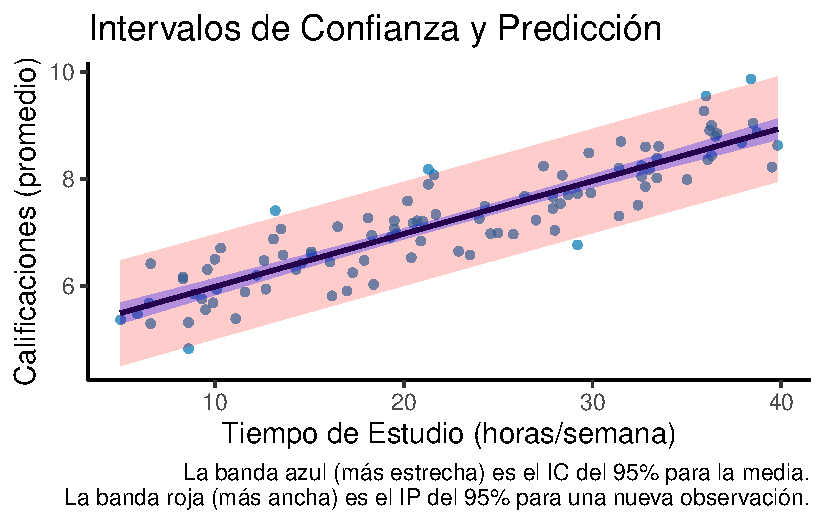
\includegraphics[keepaspectratio]{tema1_files/figure-pdf/fig-prediccion-1.pdf}}

}

\caption{\label{fig-prediccion}Comparación visual del intervalo de
confianza (azul, más estrecho) y el intervalo de predicción (rojo, más
ancho).}

\end{figure}%

El gráfico muestra claramente que la incertidumbre al predecir una
calificación individual es mucho mayor que la incertidumbre al estimar
la calificación promedio. Ambas bandas se ensanchan al alejarse del
centro de los datos.

Si quisiéramos una predicción para un estudiante que estudia 25 horas:

\begin{Shaded}
\begin{Highlighting}[]
\NormalTok{dato\_nuevo }\OtherTok{\textless{}{-}} \FunctionTok{data.frame}\NormalTok{(}\AttributeTok{Tiempo\_Estudio =} \DecValTok{25}\NormalTok{)}

\CommentTok{\# Guardamos la predicción para la media en un objeto}
\NormalTok{pred\_media }\OtherTok{\textless{}{-}} \FunctionTok{predict}\NormalTok{(modelo\_estudio, }\AttributeTok{newdata =}\NormalTok{ dato\_nuevo, }\AttributeTok{interval =} \StringTok{"confidence"}\NormalTok{)}

\CommentTok{\# Guardamos la predicción para un individuo en un objeto}
\NormalTok{pred\_indiv }\OtherTok{\textless{}{-}} \FunctionTok{predict}\NormalTok{(modelo\_estudio, }\AttributeTok{newdata =}\NormalTok{ dato\_nuevo, }\AttributeTok{interval =} \StringTok{"prediction"}\NormalTok{)}
\end{Highlighting}
\end{Shaded}

\textbf{Interpretación:}

\begin{itemize}
\tightlist
\item
  Con un 95\% de confianza, la calificación \textbf{promedio} de los
  estudiantes que estudian 25 horas está entre \textbf{7.37} y
  \textbf{7.57}.
\item
  Con un 95\% de confianza, la calificación de \textbf{un estudiante
  concreto} que estudia 25 horas estará entre \textbf{6.5} y
  \textbf{8.44}.
\end{itemize}

\end{tcolorbox}

\section{Diagnóstico del Modelo}\label{diagnuxf3stico-del-modelo}

Una vez que hemos ajustado un modelo y evaluado su significancia, el
trabajo no ha terminado. Un paso crucial, a menudo subestimado, es el
\textbf{diagnóstico del modelo} (Fox and Weisberg 2018; Harrell 2015).
Este proceso consiste en verificar si se cumplen los supuestos del
modelo de regresión lineal clásico. La fiabilidad de nuestras
inferencias (los p-valores de los contrastes t y F, y los intervalos de
confianza) depende directamente de la validez de estos supuestos.

El diagnóstico se realiza principalmente a través del \textbf{análisis
de los residuos} del modelo (\(e_i = y_i - \hat{y}_i\)). Los residuos
son nuestra mejor aproximación empírica de los errores teóricos no
observables (\(\varepsilon_i\)). A continuación, se detalla cómo
verificar cada uno de los supuestos clave.

\subsection{Linealidad}\label{linealidad}

Este supuesto establece que la relación entre la variable predictora
\(X\) y el valor esperado de la variable respuesta \(Y\) es, en
promedio, una línea recta: \(E[Y | X] = \beta_0 + \beta_1 X\).

\textbf{Métodos de diagnóstico:}

\begin{enumerate}
\def\labelenumi{\arabic{enumi}.}
\item
  \textbf{Diagnóstico visual:} El gráfico de \textbf{residuos} (\(e_i\))
  frente a los \textbf{valores ajustados} por el modelo (\(\hat{y}_i\))
  es la herramienta fundamental. La lógica es sencilla pero potente: si
  el modelo lineal es adecuado, los errores que comete (los residuos)
  deberían ser completamente aleatorios, sin guardar relación alguna con
  la magnitud de las predicciones.
\item
  \textbf{Test de Ramsey RESET:} Este test estadístico detecta
  violaciones de la forma funcional mediante la inclusión de términos no
  lineales (\(\hat{y}^2, \hat{y}^3, ...\)) en el modelo.

  \begin{itemize}
  \tightlist
  \item
    \textbf{H₀:} La forma funcional es correcta (lineal)\\
  \item
    \textbf{H₁:} La forma funcional es incorrecta (no lineal)\\
  \item
    \textbf{Estadístico:} Sigue una distribución F bajo H₀\\
  \item
    \textbf{Interpretación:} p-valor bajo indica violación de linealidad
  \end{itemize}
\end{enumerate}

\textbf{En un escenario ideal}, el gráfico debería parecer una nube de
puntos distribuida horizontalmente y sin estructura aparente, centrada
en la línea del cero. Esto nos indica que los errores son, en promedio,
nulos para todos los niveles de predicción, cumpliendo así el supuesto
de linealidad. La línea roja que R superpone en este gráfico, que
suaviza la tendencia de los puntos, debería ser prácticamente plana y
pegada al cero, confirmando la ausencia de patrones.

\begin{tcolorbox}[enhanced jigsaw, leftrule=.75mm, breakable, colbacktitle=quarto-callout-tip-color!10!white, bottomrule=.15mm, colframe=quarto-callout-tip-color-frame, toprule=.15mm, colback=white, coltitle=black, bottomtitle=1mm, left=2mm, title=\textcolor{quarto-callout-tip-color}{\faLightbulb}\hspace{0.5em}{Ejemplo de un modelo válido}, opacityback=0, arc=.35mm, opacitybacktitle=0.6, toptitle=1mm, titlerule=0mm, rightrule=.15mm]

Para nuestro \texttt{modelo\_estudio}, podemos generar específicamente
el primer gráfico de diagnóstico, que es el de Residuos vs.~Valores
Ajustados.

\begin{Shaded}
\begin{Highlighting}[]
\CommentTok{\# Crear un dataframe con los datos para ggplot2}
\FunctionTok{library}\NormalTok{(ggplot2)}
\FunctionTok{library}\NormalTok{(broom)}

\CommentTok{\# Extraer residuos y valores ajustados}
\NormalTok{datos\_diagnostico }\OtherTok{\textless{}{-}} \FunctionTok{data.frame}\NormalTok{(}
  \AttributeTok{residuos =} \FunctionTok{residuals}\NormalTok{(modelo\_estudio),}
  \AttributeTok{valores\_ajustados =} \FunctionTok{fitted}\NormalTok{(modelo\_estudio)}
\NormalTok{)}

\CommentTok{\# Gráfico de Residuos vs. Valores Ajustados con ggplot2}
\FunctionTok{ggplot}\NormalTok{(datos\_diagnostico, }\FunctionTok{aes}\NormalTok{(}\AttributeTok{x =}\NormalTok{ valores\_ajustados, }\AttributeTok{y =}\NormalTok{ residuos)) }\SpecialCharTok{+}
  \FunctionTok{geom\_point}\NormalTok{(}\AttributeTok{color =} \StringTok{"\#0072B2"}\NormalTok{, }\AttributeTok{alpha =} \FloatTok{0.7}\NormalTok{) }\SpecialCharTok{+}
  \FunctionTok{geom\_hline}\NormalTok{(}\AttributeTok{yintercept =} \DecValTok{0}\NormalTok{, }\AttributeTok{color =} \StringTok{"red"}\NormalTok{, }\AttributeTok{linetype =} \StringTok{"dashed"}\NormalTok{) }\SpecialCharTok{+}
  \FunctionTok{geom\_smooth}\NormalTok{(}\AttributeTok{method =} \StringTok{"loess"}\NormalTok{, }\AttributeTok{se =} \ConstantTok{FALSE}\NormalTok{, }\AttributeTok{color =} \StringTok{"red"}\NormalTok{, }\AttributeTok{linewidth =} \FloatTok{0.8}\NormalTok{, }\AttributeTok{formula =}\NormalTok{ y }\SpecialCharTok{\textasciitilde{}}\NormalTok{ x) }\SpecialCharTok{+}
  \FunctionTok{labs}\NormalTok{(}
    \AttributeTok{title =} \StringTok{"Residuos vs. Valores Ajustados"}\NormalTok{,}
    \AttributeTok{x =} \StringTok{"Valores Ajustados"}\NormalTok{,}
    \AttributeTok{y =} \StringTok{"Residuos"}
\NormalTok{  ) }\SpecialCharTok{+}
  \FunctionTok{theme\_classic}\NormalTok{(}\AttributeTok{base\_size =} \DecValTok{12}\NormalTok{)}
\end{Highlighting}
\end{Shaded}

\begin{figure}[H]

\centering{

\pandocbounded{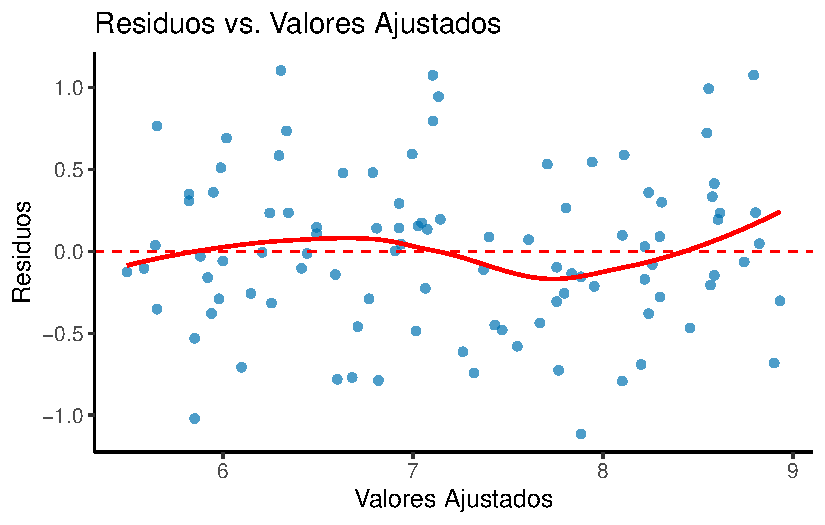
\includegraphics[keepaspectratio]{tema1_files/figure-pdf/fig-linealidad-ok-1.pdf}}

}

\caption{\label{fig-linealidad-ok}Gráfico de Residuos vs.~Valores
Ajustados para el modelo de estudio. No se observan patrones.}

\end{figure}%

Como se puede observar, los puntos se distribuyen de forma aleatoria
alrededor de la línea horizontal en cero. La línea roja, que suaviza la
tendencia de los residuos, es prácticamente plana. Esto es un claro
indicativo de que el supuesto de linealidad se cumple en nuestro modelo.

\end{tcolorbox}

Por el contrario, la aparición de un \textbf{patrón sistemático} en los
residuos es la señal de alarma de que algo anda mal. En lo que respecta
al supuesto de \textbf{linealidad}, la evidencia más clara de una
violación es una \textbf{tendencia curvilínea} (como una ``U'' o una
parábola). Este patrón nos dice que el modelo es estructuralmente
incapaz de capturar la forma de los datos y, por lo tanto, comete
errores predecibles. Por ejemplo, puede subestimar la respuesta en los
extremos (generando residuos positivos) y sobreestimarla en el centro
(residuos negativos), lo que invalida el modelo lineal.

\begin{tcolorbox}[enhanced jigsaw, leftrule=.75mm, breakable, colbacktitle=quarto-callout-tip-color!10!white, bottomrule=.15mm, colframe=quarto-callout-tip-color-frame, toprule=.15mm, colback=white, coltitle=black, bottomtitle=1mm, left=2mm, title=\textcolor{quarto-callout-tip-color}{\faLightbulb}\hspace{0.5em}{Contraejemplo: Violación del supuesto de linealidad}, opacityback=0, arc=.35mm, opacitybacktitle=0.6, toptitle=1mm, titlerule=0mm, rightrule=.15mm]

Ahora, vamos a simular a propósito unos datos que siguen una relación
cuadrática (curva) y ajustaremos incorrectamente un modelo lineal para
ver cómo se manifiesta el problema en el gráfico de diagnóstico.

\begin{Shaded}
\begin{Highlighting}[]
\CommentTok{\# 1. Simulación de datos no lineales}
\FunctionTok{set.seed}\NormalTok{(}\DecValTok{42}\NormalTok{) }\CommentTok{\# Nueva semilla para este ejemplo}
\NormalTok{x\_no\_lineal }\OtherTok{\textless{}{-}} \FunctionTok{runif}\NormalTok{(}\DecValTok{100}\NormalTok{, }\DecValTok{0}\NormalTok{, }\DecValTok{10}\NormalTok{)}
\CommentTok{\# La relación verdadera es cuadrática (y = 10 {-} (x{-}5)\^{}2) más un error}
\NormalTok{y\_no\_lineal }\OtherTok{\textless{}{-}} \DecValTok{10} \SpecialCharTok{{-}}\NormalTok{ (x\_no\_lineal }\SpecialCharTok{{-}} \DecValTok{5}\NormalTok{)}\SpecialCharTok{\^{}}\DecValTok{2} \SpecialCharTok{+} \FunctionTok{rnorm}\NormalTok{(}\DecValTok{100}\NormalTok{, }\DecValTok{0}\NormalTok{, }\DecValTok{4}\NormalTok{)}
\NormalTok{datos\_no\_lineal }\OtherTok{\textless{}{-}} \FunctionTok{data.frame}\NormalTok{(}\AttributeTok{x =}\NormalTok{ x\_no\_lineal, }\AttributeTok{y =}\NormalTok{ y\_no\_lineal)}

\CommentTok{\# 2. Ajuste de un modelo lineal (incorrecto)}
\NormalTok{modelo\_no\_lineal }\OtherTok{\textless{}{-}} \FunctionTok{lm}\NormalTok{(y }\SpecialCharTok{\textasciitilde{}}\NormalTok{ x, }\AttributeTok{data =}\NormalTok{ datos\_no\_lineal)}

\CommentTok{\# 3. Gráfico de Residuos vs. Valores Ajustados con ggplot2}
\NormalTok{datos\_diag\_no\_lineal }\OtherTok{\textless{}{-}} \FunctionTok{data.frame}\NormalTok{(}
  \AttributeTok{residuos =} \FunctionTok{residuals}\NormalTok{(modelo\_no\_lineal),}
  \AttributeTok{valores\_ajustados =} \FunctionTok{fitted}\NormalTok{(modelo\_no\_lineal)}
\NormalTok{)}

\FunctionTok{ggplot}\NormalTok{(datos\_diag\_no\_lineal, }\FunctionTok{aes}\NormalTok{(}\AttributeTok{x =}\NormalTok{ valores\_ajustados, }\AttributeTok{y =}\NormalTok{ residuos)) }\SpecialCharTok{+}
  \FunctionTok{geom\_point}\NormalTok{(}\AttributeTok{color =} \StringTok{"\#D55E00"}\NormalTok{, }\AttributeTok{alpha =} \FloatTok{0.7}\NormalTok{) }\SpecialCharTok{+}
  \FunctionTok{geom\_hline}\NormalTok{(}\AttributeTok{yintercept =} \DecValTok{0}\NormalTok{, }\AttributeTok{color =} \StringTok{"red"}\NormalTok{, }\AttributeTok{linetype =} \StringTok{"dashed"}\NormalTok{) }\SpecialCharTok{+}
  \FunctionTok{geom\_smooth}\NormalTok{(}\AttributeTok{method =} \StringTok{"loess"}\NormalTok{, }\AttributeTok{se =} \ConstantTok{FALSE}\NormalTok{, }\AttributeTok{color =} \StringTok{"red"}\NormalTok{, }\AttributeTok{linewidth =} \FloatTok{0.8}\NormalTok{, }\AttributeTok{formula =}\NormalTok{ y }\SpecialCharTok{\textasciitilde{}}\NormalTok{ x) }\SpecialCharTok{+}
  \FunctionTok{labs}\NormalTok{(}
    \AttributeTok{title =} \StringTok{"Residuos vs. Valores Ajustados (Violación de Linealidad)"}\NormalTok{,}
    \AttributeTok{x =} \StringTok{"Valores Ajustados"}\NormalTok{,}
    \AttributeTok{y =} \StringTok{"Residuos"}
\NormalTok{  ) }\SpecialCharTok{+}
  \FunctionTok{theme\_classic}\NormalTok{(}\AttributeTok{base\_size =} \DecValTok{12}\NormalTok{)}
\end{Highlighting}
\end{Shaded}

\begin{figure}[H]

\centering{

\pandocbounded{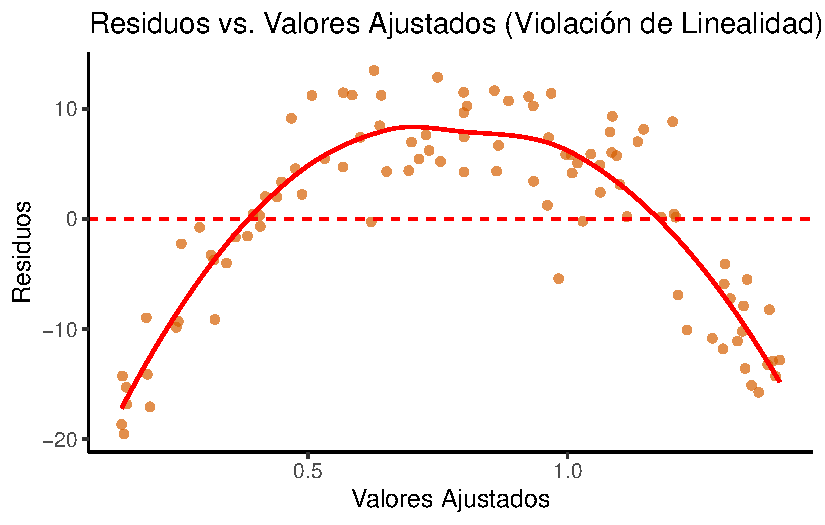
\includegraphics[keepaspectratio]{tema1_files/figure-pdf/fig-linealidad-mal-1.pdf}}

}

\caption{\label{fig-linealidad-mal}Patrón curvo evidente en los
residuos, violando el supuesto de linealidad.}

\end{figure}%

El gráfico de diagnóstico es inequívoco. A diferencia del ejemplo
anterior, donde los puntos formaban una nube aleatoria, aquí los
residuos dibujan un \textbf{patrón parabólico} perfecto (una ``U''
invertida). La línea roja de tendencia, en lugar de ser plana, sigue
fielmente esta curva.

\textbf{Test de Ramsey RESET para Linealidad}

Además del diagnóstico visual, podemos usar el test de Ramsey RESET
(Regression Equation Specification Error Test) para detectar violaciones
de linealidad:

\begin{Shaded}
\begin{Highlighting}[]
\FunctionTok{suppressPackageStartupMessages}\NormalTok{(}\FunctionTok{library}\NormalTok{(lmtest))}
\CommentTok{\# Test RESET para el modelo correcto (horas de estudio)}
\NormalTok{reset\_resultado }\OtherTok{\textless{}{-}} \FunctionTok{resettest}\NormalTok{(modelo\_estudio, }\AttributeTok{power =} \DecValTok{2}\SpecialCharTok{:}\DecValTok{3}\NormalTok{, }\AttributeTok{type =} \StringTok{"fitted"}\NormalTok{)}
\FunctionTok{print}\NormalTok{(reset\_resultado)}
\end{Highlighting}
\end{Shaded}

\begin{verbatim}

    RESET test

data:  modelo_estudio
RESET = 1.0513, df1 = 2, df2 = 96, p-value = 0.3535
\end{verbatim}

\begin{Shaded}
\begin{Highlighting}[]
\CommentTok{\# Test RESET para el modelo incorrecto (no lineal)}
\NormalTok{reset\_no\_lineal }\OtherTok{\textless{}{-}} \FunctionTok{resettest}\NormalTok{(modelo\_no\_lineal, }\AttributeTok{power =} \DecValTok{2}\SpecialCharTok{:}\DecValTok{3}\NormalTok{, }\AttributeTok{type =} \StringTok{"fitted"}\NormalTok{)}
\FunctionTok{print}\NormalTok{(reset\_no\_lineal)}
\end{Highlighting}
\end{Shaded}

\begin{verbatim}

    RESET test

data:  modelo_no_lineal
RESET = 231.9, df1 = 2, df2 = 96, p-value < 2.2e-16
\end{verbatim}

El test de Ramsey RESET confirma nuestro diagnóstico visual:

\begin{itemize}
\tightlist
\item
  Para el modelo correcto: p-valor = 0.3535 → No rechazamos H₀ (forma
  funcional correcta)
\item
  Para el modelo no lineal: p-valor = 0 → Rechazamos H₀ (forma funcional
  incorrecta)
\end{itemize}

\end{tcolorbox}

\subsection{Homocedasticidad}\label{homocedasticidad}

El supuesto de homocedasticidad establece que la varianza de los errores
del modelo debe ser constante para todos los niveles de la variable
predictora. Es decir, la dispersión de los datos alrededor de la línea
de regresión es la misma en todo su recorrido
(\(Var(\varepsilon_i | X_i) = \sigma^2\)). La violación de este supuesto
se conoce como \textbf{heterocedasticidad}, y es un problema común en el
modelado.

\textbf{Métodos de diagnóstico:}

\begin{enumerate}
\def\labelenumi{\arabic{enumi}.}
\item
  \textbf{Diagnóstico visual:} El gráfico \textbf{Scale-Location}
  muestra la raíz cuadrada de los residuos estandarizados absolutos
  frente a los valores ajustados. Una línea horizontal indica
  homocedasticidad.
\item
  \textbf{Test de Breusch-Pagan:} Test clásico para detectar
  heterocedasticidad.

  \begin{itemize}
  \tightlist
  \item
    \textbf{H₀:} Homocedasticidad (varianza constante)
  \item
    \textbf{H₁:} Heterocedasticidad
  \item
    \textbf{Estadístico:} LM \textasciitilde{} χ² bajo H₀
  \end{itemize}
\item
  \textbf{Test de White:} Versión más robusta que no asume una forma
  específica de heterocedasticidad.

  \begin{itemize}
  \tightlist
  \item
    \textbf{H₀:} Homocedasticidad
  \item
    \textbf{H₁:} Heterocedasticidad (forma general)
  \item
    \textbf{Ventaja:} No requiere especificar la forma funcional de la
    heterocedasticidad
  \end{itemize}
\end{enumerate}

¿Por qué es tan importante? Si un modelo es heteroscedástico, los
errores estándar de los coeficientes (\(\beta_0, \beta_1\)) estarán
calculados de forma incorrecta. Como consecuencia, los intervalos de
confianza y los contrastes de hipótesis (p-valores) no serán fiables,
pudiendo llevarnos a conclusiones erróneas sobre la significancia de
nuestras variables.

\begin{tcolorbox}[enhanced jigsaw, leftrule=.75mm, breakable, colbacktitle=quarto-callout-note-color!10!white, bottomrule=.15mm, colframe=quarto-callout-note-color-frame, toprule=.15mm, colback=white, coltitle=black, bottomtitle=1mm, left=2mm, title=\textcolor{quarto-callout-note-color}{\faInfo}\hspace{0.5em}{Sobre los residuos estandarizados}, opacityback=0, arc=.35mm, opacitybacktitle=0.6, toptitle=1mm, titlerule=0mm, rightrule=.15mm]

Los \textbf{residuos simples} (\(e_i = y_i - \hat{y}_i\)) no son
directamente comparables entre sí porque tienen diferentes varianzas
dependiendo de su apalancamiento (\emph{leverage}). Por eso, en los
gráficos de diagnóstico se utilizan \textbf{residuos estandarizados} o,
mejor aún, \textbf{residuos estudentizados}, que ponen todos los
residuos en una escala común. Esto facilita la identificación de
patrones y valores atípicos. La explicación detallada de estos conceptos
se encuentra en la sección de identificación de observaciones
influyentes.

\end{tcolorbox}

La heteroscedasticidad se detecta principalmente buscando patrones en la
dispersión de los residuos.

\begin{itemize}
\item
  \textbf{Gráfico de Residuos vs.~Valores Ajustados:} Como en la prueba
  de linealidad, este gráfico es nuestra primera herramienta. Aquí no
  buscamos patrones en la media de los residuos (que debe ser cero),
  sino en su \textbf{dispersión}. La señal de alarma inequívoca de
  heteroscedasticidad es una \textbf{forma de embudo o megáfono}, donde
  la dispersión de los residuos aumenta o disminuye a medida que cambian
  los valores ajustados.
\item
  \textbf{Gráfico Scale-Location:} Este gráfico está diseñado
  específicamente para detectar heteroscedasticidad. Muestra la raíz
  cuadrada de los residuos estandarizados en el eje Y
  (\texttt{sqrt(\textbar{}Standardized\ residuals\textbar{})}) frente a
  los valores ajustados en el eje X. Al usar la raíz cuadrada, se
  suaviza la distribución de los residuos, haciendo los patrones de
  varianza más fáciles de ver. Si la varianza es constante
  (homocedasticidad), deberíamos ver una nube de puntos aleatoria con
  una línea de tendencia roja aproximadamente plana. Una pendiente en
  esta línea roja indica que la varianza cambia con el nivel de la
  respuesta.
\item
  \textbf{Prueba de Breusch-Pagan:} Es el contraste de hipótesis formal.
  Su lógica es ingeniosa: realiza una regresión auxiliar donde intenta
  predecir los residuos al cuadrado a partir de las variables
  predictoras originales. Si las variables predictoras ayudan a explicar
  la magnitud de los residuos al cuadrado, significa que la varianza del
  error depende de los predictores, y por tanto, hay
  heteroscedasticidad.

  \begin{itemize}
  \tightlist
  \item
    \textbf{Hipótesis Nula (}\(H_0\)): El modelo es homocedástico.
  \item
    \textbf{Decisión:} Un p-valor pequeño (p.~ej., \textless{} 0.05) es
    evidencia en contra de la homocedasticidad.
  \end{itemize}
\end{itemize}

\begin{tcolorbox}[enhanced jigsaw, leftrule=.75mm, breakable, colbacktitle=quarto-callout-tip-color!10!white, bottomrule=.15mm, colframe=quarto-callout-tip-color-frame, toprule=.15mm, colback=white, coltitle=black, bottomtitle=1mm, left=2mm, title=\textcolor{quarto-callout-tip-color}{\faLightbulb}\hspace{0.5em}{Ejemplo de un modelo válido}, opacityback=0, arc=.35mm, opacitybacktitle=0.6, toptitle=1mm, titlerule=0mm, rightrule=.15mm]

Analicemos nuestro \texttt{modelo\_estudio}. Nos centraremos en el
gráfico \texttt{Scale-Location} (\texttt{which\ =\ 3}) y en la prueba de
Breusch-Pagan.

\begin{Shaded}
\begin{Highlighting}[]
\CommentTok{\# Crear datos para el gráfico Scale{-}Location}
\NormalTok{datos\_scale\_loc }\OtherTok{\textless{}{-}} \FunctionTok{data.frame}\NormalTok{(}
  \AttributeTok{valores\_ajustados =} \FunctionTok{fitted}\NormalTok{(modelo\_estudio),}
  \AttributeTok{residuos\_std\_sqrt =} \FunctionTok{sqrt}\NormalTok{(}\FunctionTok{abs}\NormalTok{(}\FunctionTok{rstandard}\NormalTok{(modelo\_estudio)))}
\NormalTok{)}

\CommentTok{\# Gráfico Scale{-}Location con ggplot2}
\FunctionTok{ggplot}\NormalTok{(datos\_scale\_loc, }\FunctionTok{aes}\NormalTok{(}\AttributeTok{x =}\NormalTok{ valores\_ajustados, }\AttributeTok{y =}\NormalTok{ residuos\_std\_sqrt)) }\SpecialCharTok{+}
  \FunctionTok{geom\_point}\NormalTok{(}\AttributeTok{color =} \StringTok{"\#0072B2"}\NormalTok{, }\AttributeTok{alpha =} \FloatTok{0.7}\NormalTok{) }\SpecialCharTok{+}
  \FunctionTok{geom\_smooth}\NormalTok{(}\AttributeTok{method =} \StringTok{"loess"}\NormalTok{, }\AttributeTok{se =} \ConstantTok{FALSE}\NormalTok{, }\AttributeTok{color =} \StringTok{"red"}\NormalTok{, }\AttributeTok{linewidth =} \FloatTok{0.8}\NormalTok{, }\AttributeTok{formula =}\NormalTok{ y }\SpecialCharTok{\textasciitilde{}}\NormalTok{ x) }\SpecialCharTok{+}
  \FunctionTok{labs}\NormalTok{(}
    \AttributeTok{title =} \StringTok{"Scale{-}Location"}\NormalTok{,}
    \AttributeTok{x =} \StringTok{"Valores Ajustados"}\NormalTok{,}
    \AttributeTok{y =} \FunctionTok{expression}\NormalTok{(}\FunctionTok{sqrt}\NormalTok{(}\StringTok{"|Residuos Estandarizados|"}\NormalTok{))}
\NormalTok{  ) }\SpecialCharTok{+}
  \FunctionTok{theme\_classic}\NormalTok{(}\AttributeTok{base\_size =} \DecValTok{12}\NormalTok{)}

\CommentTok{\# Prueba de Breusch{-}Pagan}
\FunctionTok{suppressPackageStartupMessages}\NormalTok{(}\FunctionTok{library}\NormalTok{(lmtest))}
\NormalTok{bp\_resultado }\OtherTok{\textless{}{-}} \FunctionTok{bptest}\NormalTok{(modelo\_estudio)}
\FunctionTok{print}\NormalTok{(bp\_resultado)}
\end{Highlighting}
\end{Shaded}

\begin{verbatim}

    studentized Breusch-Pagan test

data:  modelo_estudio
BP = 0.019638, df = 1, p-value = 0.8886
\end{verbatim}

\begin{Shaded}
\begin{Highlighting}[]
\CommentTok{\# Prueba de White (versión robusta)}
\NormalTok{white\_resultado }\OtherTok{\textless{}{-}} \FunctionTok{bptest}\NormalTok{(modelo\_estudio, }\SpecialCharTok{\textasciitilde{}} \FunctionTok{fitted}\NormalTok{(modelo\_estudio) }\SpecialCharTok{+} \FunctionTok{I}\NormalTok{(}\FunctionTok{fitted}\NormalTok{(modelo\_estudio)}\SpecialCharTok{\^{}}\DecValTok{2}\NormalTok{))}
\FunctionTok{print}\NormalTok{(white\_resultado)}
\end{Highlighting}
\end{Shaded}

\begin{verbatim}

    studentized Breusch-Pagan test

data:  modelo_estudio
BP = 0.12238, df = 2, p-value = 0.9406
\end{verbatim}

\begin{figure}[H]

\centering{

\pandocbounded{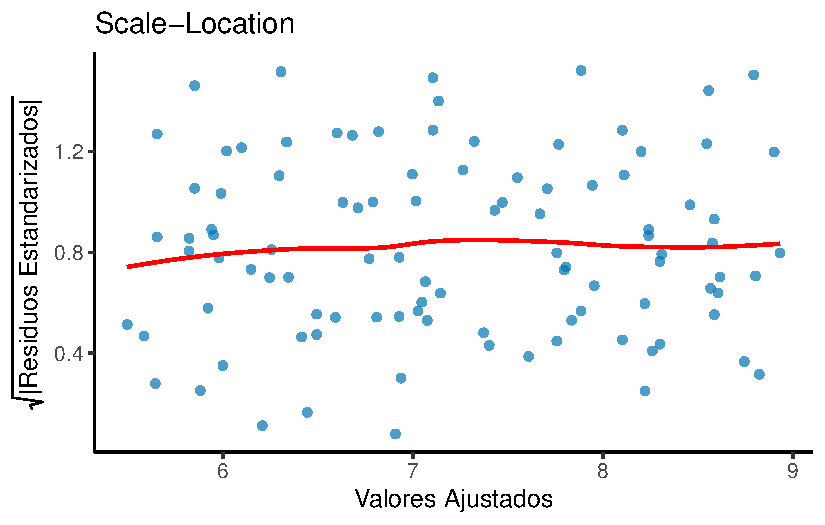
\includegraphics[keepaspectratio]{tema1_files/figure-pdf/fig-homocedasticidad-ok-1.pdf}}

}

\caption{\label{fig-homocedasticidad-ok}Gráfico Scale-Location para el
modelo de estudio. La línea de tendencia es casi plana.}

\end{figure}%

El diagnóstico es positivo. En el gráfico \texttt{Scale-Location}, la
línea roja es casi horizontal, lo que indica que la varianza de los
residuos es estable a lo largo de los valores ajustados. Esto se
confirma con ambas pruebas:

\begin{itemize}
\tightlist
\item
  \textbf{Breusch-Pagan}: p-valor = 0.8886 → No rechazamos H₀
  (homocedasticidad)
\item
  \textbf{White}: p-valor = 0.9406 → No rechazamos H₀ (varianza
  constante) \textbf{Nuestro modelo cumple el supuesto}.
\end{itemize}

\end{tcolorbox}

\begin{tcolorbox}[enhanced jigsaw, leftrule=.75mm, breakable, colbacktitle=quarto-callout-tip-color!10!white, bottomrule=.15mm, colframe=quarto-callout-tip-color-frame, toprule=.15mm, colback=white, coltitle=black, bottomtitle=1mm, left=2mm, title=\textcolor{quarto-callout-tip-color}{\faLightbulb}\hspace{0.5em}{Contraejemplo: Violación del supuesto de homocedasticidad}, opacityback=0, arc=.35mm, opacitybacktitle=0.6, toptitle=1mm, titlerule=0mm, rightrule=.15mm]

Ahora, simularemos datos donde el error aumenta a medida que \texttt{x}
crece, un caso clásico de heteroscedasticidad.

\begin{Shaded}
\begin{Highlighting}[]
\CommentTok{\# 1. Simulación de datos heteroscedásticos}
\FunctionTok{set.seed}\NormalTok{(}\DecValTok{101}\NormalTok{)}
\NormalTok{x\_hetero }\OtherTok{\textless{}{-}} \DecValTok{1}\SpecialCharTok{:}\DecValTok{100}
\NormalTok{y\_hetero }\OtherTok{\textless{}{-}} \DecValTok{10} \SpecialCharTok{+} \DecValTok{2} \SpecialCharTok{*}\NormalTok{ x\_hetero }\SpecialCharTok{+} \FunctionTok{rnorm}\NormalTok{(}\DecValTok{100}\NormalTok{, }\AttributeTok{mean =} \DecValTok{0}\NormalTok{, }\AttributeTok{sd =} \FloatTok{0.4} \SpecialCharTok{*}\NormalTok{ x\_hetero)}
\NormalTok{datos\_hetero }\OtherTok{\textless{}{-}} \FunctionTok{data.frame}\NormalTok{(}\AttributeTok{x =}\NormalTok{ x\_hetero, }\AttributeTok{y =}\NormalTok{ y\_hetero)}
\NormalTok{modelo\_hetero }\OtherTok{\textless{}{-}} \FunctionTok{lm}\NormalTok{(y }\SpecialCharTok{\textasciitilde{}}\NormalTok{ x, }\AttributeTok{data =}\NormalTok{ datos\_hetero)}

\CommentTok{\# 2. Preparar datos para los gráficos}
\NormalTok{datos\_diag\_hetero }\OtherTok{\textless{}{-}} \FunctionTok{data.frame}\NormalTok{(}
  \AttributeTok{residuos =} \FunctionTok{residuals}\NormalTok{(modelo\_hetero),}
  \AttributeTok{valores\_ajustados =} \FunctionTok{fitted}\NormalTok{(modelo\_hetero),}
  \AttributeTok{residuos\_std\_sqrt =} \FunctionTok{sqrt}\NormalTok{(}\FunctionTok{abs}\NormalTok{(}\FunctionTok{rstandard}\NormalTok{(modelo\_hetero)))}
\NormalTok{)}

\CommentTok{\# 3. Gráfico de Residuos vs. Valores Ajustados}
\NormalTok{p1 }\OtherTok{\textless{}{-}} \FunctionTok{ggplot}\NormalTok{(datos\_diag\_hetero, }\FunctionTok{aes}\NormalTok{(}\AttributeTok{x =}\NormalTok{ valores\_ajustados, }\AttributeTok{y =}\NormalTok{ residuos)) }\SpecialCharTok{+}
  \FunctionTok{geom\_point}\NormalTok{(}\AttributeTok{color =} \StringTok{"\#D55E00"}\NormalTok{, }\AttributeTok{alpha =} \FloatTok{0.7}\NormalTok{) }\SpecialCharTok{+}
  \FunctionTok{geom\_hline}\NormalTok{(}\AttributeTok{yintercept =} \DecValTok{0}\NormalTok{, }\AttributeTok{color =} \StringTok{"red"}\NormalTok{, }\AttributeTok{linetype =} \StringTok{"dashed"}\NormalTok{) }\SpecialCharTok{+}
  \FunctionTok{geom\_smooth}\NormalTok{(}\AttributeTok{method =} \StringTok{"loess"}\NormalTok{, }\AttributeTok{se =} \ConstantTok{FALSE}\NormalTok{, }\AttributeTok{color =} \StringTok{"red"}\NormalTok{, }\AttributeTok{linewidth =} \FloatTok{0.8}\NormalTok{, }\AttributeTok{formula =}\NormalTok{ y }\SpecialCharTok{\textasciitilde{}}\NormalTok{ x) }\SpecialCharTok{+}
  \FunctionTok{labs}\NormalTok{(}
    \AttributeTok{title =} \StringTok{"Residuos vs. Valores Ajustados"}\NormalTok{,}
    \AttributeTok{x =} \StringTok{"Valores Ajustados"}\NormalTok{,}
    \AttributeTok{y =} \StringTok{"Residuos"}
\NormalTok{  ) }\SpecialCharTok{+}
  \FunctionTok{theme\_classic}\NormalTok{(}\AttributeTok{base\_size =} \DecValTok{10}\NormalTok{)}

\CommentTok{\# 4. Gráfico Scale{-}Location}
\NormalTok{p2 }\OtherTok{\textless{}{-}} \FunctionTok{ggplot}\NormalTok{(datos\_diag\_hetero, }\FunctionTok{aes}\NormalTok{(}\AttributeTok{x =}\NormalTok{ valores\_ajustados, }\AttributeTok{y =}\NormalTok{ residuos\_std\_sqrt)) }\SpecialCharTok{+}
  \FunctionTok{geom\_point}\NormalTok{(}\AttributeTok{color =} \StringTok{"\#D55E00"}\NormalTok{, }\AttributeTok{alpha =} \FloatTok{0.7}\NormalTok{) }\SpecialCharTok{+}
  \FunctionTok{geom\_smooth}\NormalTok{(}\AttributeTok{method =} \StringTok{"loess"}\NormalTok{, }\AttributeTok{se =} \ConstantTok{FALSE}\NormalTok{, }\AttributeTok{color =} \StringTok{"red"}\NormalTok{, }\AttributeTok{linewidth =} \FloatTok{0.8}\NormalTok{, }\AttributeTok{formula =}\NormalTok{ y }\SpecialCharTok{\textasciitilde{}}\NormalTok{ x) }\SpecialCharTok{+}
  \FunctionTok{labs}\NormalTok{(}
    \AttributeTok{title =} \StringTok{"Scale{-}Location"}\NormalTok{,}
    \AttributeTok{x =} \StringTok{"Valores Ajustados"}\NormalTok{,}
    \AttributeTok{y =} \FunctionTok{expression}\NormalTok{(}\FunctionTok{sqrt}\NormalTok{(}\StringTok{"|Residuos Estandarizados|"}\NormalTok{))}
\NormalTok{  ) }\SpecialCharTok{+}
  \FunctionTok{theme\_classic}\NormalTok{(}\AttributeTok{base\_size =} \DecValTok{10}\NormalTok{)}

\CommentTok{\# 5. Mostrar ambos gráficos lado a lado}
\FunctionTok{library}\NormalTok{(gridExtra)}
\FunctionTok{grid.arrange}\NormalTok{(p1, p2, }\AttributeTok{ncol =} \DecValTok{2}\NormalTok{)}

\CommentTok{\# 6. Prueba de Breusch{-}Pagan}
\FunctionTok{suppressPackageStartupMessages}\NormalTok{(}\FunctionTok{library}\NormalTok{(lmtest))}
\NormalTok{test\_values }\OtherTok{\textless{}{-}} \FunctionTok{bptest}\NormalTok{(modelo\_hetero)}
\end{Highlighting}
\end{Shaded}

\begin{figure}[H]

\centering{

\pandocbounded{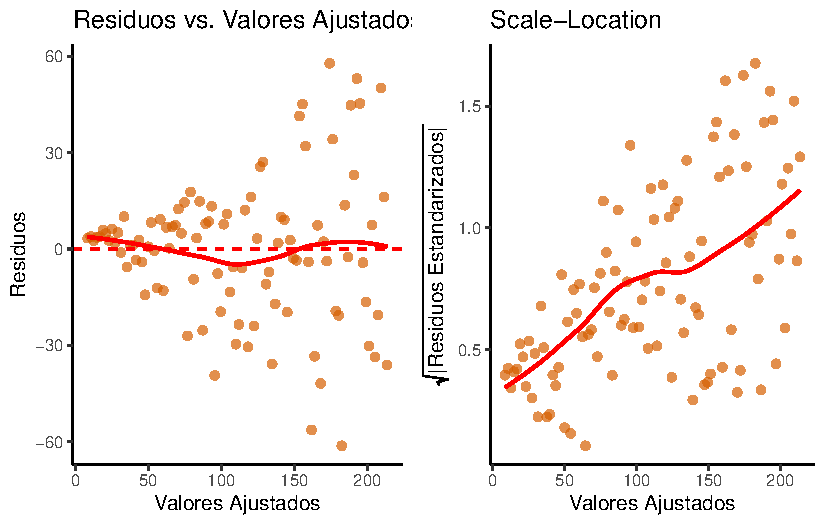
\includegraphics[keepaspectratio]{tema1_files/figure-pdf/fig-homocedasticidad-mal-1.pdf}}

}

\caption{\label{fig-homocedasticidad-mal}Diagnóstico de
heteroscedasticidad. Izquierda: Gráfico de Residuos vs.~Ajustados
(patrón de embudo). Derecha: Gráfico Scale-Location (tendencia
ascendente).}

\end{figure}%

Los resultados son un libro de texto sobre la heteroscedasticidad.

\begin{itemize}
\tightlist
\item
  El gráfico de \textbf{Residuos vs.~Valores Ajustados} (izquierda)
  tiene una \textbf{forma de embudo} inconfundible: la dispersión de los
  puntos aumenta drásticamente de izquierda a derecha.
\item
  El gráfico \textbf{Scale-Location} (derecha) confirma el problema,
  mostrando una línea roja con una \textbf{clara pendiente ascendente}.
\item
  La \textbf{prueba de Breusch-Pagan} arroja un \textbf{p-valor
  7.43e-07}, dándonos una fuerte evidencia estadística para rechazar la
  hipótesis nula de homocedasticidad.
\end{itemize}

Este modelo viola claramente el supuesto, y las inferencias basadas en
él (como el p-valor del coeficiente de \texttt{x}) no serían fiables.

\end{tcolorbox}

\subsection{Normalidad de los
residuos}\label{normalidad-de-los-residuos}

Este supuesto postula que los residuos del modelo (\(\varepsilon_i\))
siguen una distribución normal: \(\varepsilon_i \sim N(0, \sigma^2)\).
Es especialmente importante para la validez de los intervalos de
confianza y los contrastes de hipótesis cuando el tamaño de la muestra
es pequeño.

\textbf{Métodos de diagnóstico:}

\begin{enumerate}
\def\labelenumi{\arabic{enumi}.}
\item
  \textbf{Diagnóstico visual:}

  \begin{itemize}
  \tightlist
  \item
    \textbf{Gráfico Q-Q:} Los puntos deben seguir la línea diagonal si
    hay normalidad
  \item
    \textbf{Histograma:} Debe mostrar forma campaniforme y simétrica
  \end{itemize}
\item
  \textbf{Test de Shapiro-Wilk:} Test más potente para muestras pequeñas
  y medianas (n \textless{} 50).

  \begin{itemize}
  \tightlist
  \item
    \textbf{H₀:} Los residuos siguen distribución normal
  \item
    \textbf{H₁:} Los residuos no siguen distribución normal
  \item
    \textbf{Limitación:} Muy sensible en muestras grandes
  \end{itemize}
\item
  \textbf{Test de Jarque-Bera:} Basado en medidas de asimetría y
  curtosis.

  \begin{itemize}
  \tightlist
  \item
    \textbf{H₀:} Los residuos son normales (asimetría = 0, curtosis = 3)
  \item
    \textbf{H₁:} Los residuos no son normales
  \item
    \textbf{Ventaja:} Menos sensible al tamaño muestral que Shapiro-Wilk
  \end{itemize}
\end{enumerate}

Para evaluar la normalidad disponemos de estas herramientas visuales y
analíticas:

\begin{itemize}
\tightlist
\item
  \textbf{Gráfico Normal Q-Q (\texttt{Normal\ Q-Q\ Plot}):} Compara los
  cuantiles de los residuos estandarizados con los cuantiles de una
  distribución normal teórica. Los puntos deben caer muy cerca de la
  línea diagonal de 45 grados.
\item
  \textbf{Histograma de los Residuos:} Un simple histograma de los
  residuos debe mostrar una forma aproximada de campana de Gauss.
\item
  \textbf{Prueba de Shapiro-Wilk:} Es uno de los contrastes más potentes
  para la normalidad.

  \begin{itemize}
  \tightlist
  \item
    \textbf{Hipótesis Nula (}\(H_0\)): Los residuos provienen de una
    distribución normal.
  \item
    \textbf{Decisión:} Un p-valor pequeño (\textless{} 0.05) sugiere
    rechazar \(H_0\).
  \end{itemize}
\end{itemize}

\begin{tcolorbox}[enhanced jigsaw, leftrule=.75mm, breakable, colbacktitle=quarto-callout-tip-color!10!white, bottomrule=.15mm, colframe=quarto-callout-tip-color-frame, toprule=.15mm, colback=white, coltitle=black, bottomtitle=1mm, left=2mm, title=\textcolor{quarto-callout-tip-color}{\faLightbulb}\hspace{0.5em}{Ejemplo de normalidad válida}, opacityback=0, arc=.35mm, opacitybacktitle=0.6, toptitle=1mm, titlerule=0mm, rightrule=.15mm]

Para nuestro \texttt{modelo\_estudio}, examinamos la normalidad mediante
el gráfico Q-Q y la prueba de Shapiro-Wilk.

\begin{Shaded}
\begin{Highlighting}[]
\CommentTok{\# Crear datos para los gráficos}
\NormalTok{residuos }\OtherTok{\textless{}{-}} \FunctionTok{residuals}\NormalTok{(modelo\_estudio)}

\CommentTok{\# 1. Gráfico Q{-}Q con ggplot2}
\NormalTok{datos\_qq }\OtherTok{\textless{}{-}} \FunctionTok{data.frame}\NormalTok{(}\AttributeTok{residuos =}\NormalTok{ residuos)}

\NormalTok{p1 }\OtherTok{\textless{}{-}} \FunctionTok{ggplot}\NormalTok{(datos\_qq, }\FunctionTok{aes}\NormalTok{(}\AttributeTok{sample =}\NormalTok{ residuos)) }\SpecialCharTok{+}
  \FunctionTok{geom\_qq}\NormalTok{(}\AttributeTok{color =} \StringTok{"\#0072B2"}\NormalTok{, }\AttributeTok{alpha =} \FloatTok{0.7}\NormalTok{) }\SpecialCharTok{+}
  \FunctionTok{geom\_qq\_line}\NormalTok{(}\AttributeTok{color =} \StringTok{"red"}\NormalTok{, }\AttributeTok{linetype =} \StringTok{"dashed"}\NormalTok{) }\SpecialCharTok{+}
  \FunctionTok{labs}\NormalTok{(}
    \AttributeTok{title =} \StringTok{"Normal Q{-}Q Plot"}\NormalTok{,}
    \AttributeTok{x =} \StringTok{"Cuantiles Teóricos"}\NormalTok{,}
    \AttributeTok{y =} \StringTok{"Cuantiles de la Muestra"}
\NormalTok{  ) }\SpecialCharTok{+}
  \FunctionTok{theme\_classic}\NormalTok{(}\AttributeTok{base\_size =} \DecValTok{10}\NormalTok{)}

\CommentTok{\# 2. Histograma con ggplot2}
\NormalTok{datos\_hist }\OtherTok{\textless{}{-}} \FunctionTok{data.frame}\NormalTok{(}\AttributeTok{residuos =}\NormalTok{ residuos)}

\NormalTok{p2 }\OtherTok{\textless{}{-}} \FunctionTok{ggplot}\NormalTok{(datos\_hist, }\FunctionTok{aes}\NormalTok{(}\AttributeTok{x =}\NormalTok{ residuos)) }\SpecialCharTok{+}
  \FunctionTok{geom\_histogram}\NormalTok{(}\FunctionTok{aes}\NormalTok{(}\AttributeTok{y =} \FunctionTok{after\_stat}\NormalTok{(density)), }\AttributeTok{bins =} \DecValTok{15}\NormalTok{, }\AttributeTok{fill =} \StringTok{"lightblue"}\NormalTok{, }
                 \AttributeTok{color =} \StringTok{"black"}\NormalTok{, }\AttributeTok{alpha =} \FloatTok{0.7}\NormalTok{) }\SpecialCharTok{+}
  \FunctionTok{stat\_function}\NormalTok{(}\AttributeTok{fun =}\NormalTok{ dnorm, }
                \AttributeTok{args =} \FunctionTok{list}\NormalTok{(}\AttributeTok{mean =} \FunctionTok{mean}\NormalTok{(residuos), }\AttributeTok{sd =} \FunctionTok{sd}\NormalTok{(residuos)),}
                \AttributeTok{color =} \StringTok{"red"}\NormalTok{, }\AttributeTok{linewidth =} \DecValTok{1}\NormalTok{) }\SpecialCharTok{+}
  \FunctionTok{labs}\NormalTok{(}
    \AttributeTok{title =} \StringTok{"Histograma de Residuos"}\NormalTok{,}
    \AttributeTok{x =} \StringTok{"Residuos"}\NormalTok{,}
    \AttributeTok{y =} \StringTok{"Densidad"}
\NormalTok{  ) }\SpecialCharTok{+}
  \FunctionTok{theme\_classic}\NormalTok{(}\AttributeTok{base\_size =} \DecValTok{10}\NormalTok{)}

\CommentTok{\# 3. Mostrar ambos gráficos lado a lado}
\FunctionTok{library}\NormalTok{(gridExtra)}
\FunctionTok{grid.arrange}\NormalTok{(p1, p2, }\AttributeTok{ncol =} \DecValTok{2}\NormalTok{)}

\CommentTok{\# Prueba de Shapiro{-}Wilk}
\FunctionTok{suppressPackageStartupMessages}\NormalTok{(}\FunctionTok{library}\NormalTok{(lmtest))}
\NormalTok{shapiro\_resultado }\OtherTok{\textless{}{-}} \FunctionTok{shapiro.test}\NormalTok{(}\FunctionTok{residuals}\NormalTok{(modelo\_estudio))}
\FunctionTok{print}\NormalTok{(shapiro\_resultado)}
\end{Highlighting}
\end{Shaded}

\begin{verbatim}

    Shapiro-Wilk normality test

data:  residuals(modelo_estudio)
W = 0.99008, p-value = 0.671
\end{verbatim}

\begin{Shaded}
\begin{Highlighting}[]
\CommentTok{\# Prueba de Jarque{-}Bera}
\FunctionTok{suppressPackageStartupMessages}\NormalTok{(}\FunctionTok{library}\NormalTok{(tseries))}
\NormalTok{jb\_resultado }\OtherTok{\textless{}{-}} \FunctionTok{jarque.bera.test}\NormalTok{(}\FunctionTok{residuals}\NormalTok{(modelo\_estudio))}
\FunctionTok{print}\NormalTok{(jb\_resultado)}
\end{Highlighting}
\end{Shaded}

\begin{verbatim}

    Jarque Bera Test

data:  residuals(modelo_estudio)
X-squared = 0.68515, df = 2, p-value = 0.7099
\end{verbatim}

\begin{figure}[H]

\centering{

\pandocbounded{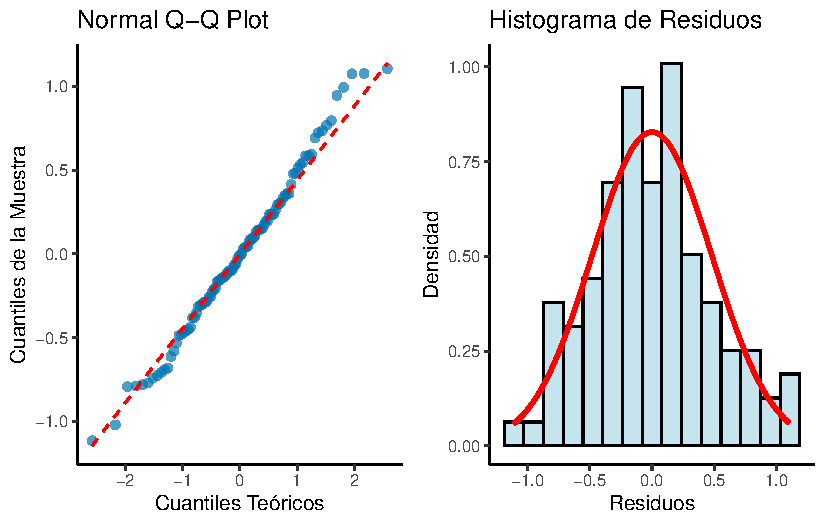
\includegraphics[keepaspectratio]{tema1_files/figure-pdf/fig-normalidad-ok-1.pdf}}

}

\caption{\label{fig-normalidad-ok}Diagnóstico de normalidad del modelo
de estudio. Izquierda: Q-Q Plot. Derecha: Histograma de residuos.}

\end{figure}%

El diagnóstico es excelente. En el gráfico Q-Q, los puntos se alinean
muy bien con la línea diagonal, indicando normalidad. El histograma
muestra una distribución aproximadamente simétrica que se ajusta bien a
la curva normal teórica (línea roja). Ambas pruebas estadísticas
confirman la normalidad:

\begin{itemize}
\tightlist
\item
  \textbf{Shapiro-Wilk}: p-valor = 0.671 → No rechazamos H₀ (normalidad)
\item
  \textbf{Jarque-Bera}: p-valor = 0.7099 → No rechazamos H₀ (normalidad)
\end{itemize}

\end{tcolorbox}

\begin{tcolorbox}[enhanced jigsaw, leftrule=.75mm, breakable, colbacktitle=quarto-callout-tip-color!10!white, bottomrule=.15mm, colframe=quarto-callout-tip-color-frame, toprule=.15mm, colback=white, coltitle=black, bottomtitle=1mm, left=2mm, title=\textcolor{quarto-callout-tip-color}{\faLightbulb}\hspace{0.5em}{Contraejemplo: Violación del supuesto de normalidad}, opacityback=0, arc=.35mm, opacitybacktitle=0.6, toptitle=1mm, titlerule=0mm, rightrule=.15mm]

Ahora simularemos datos donde los residuos siguen una distribución
asimétrica (distribución exponencial) para mostrar una violación clara
del supuesto de normalidad.

\begin{Shaded}
\begin{Highlighting}[]
\CommentTok{\# 1. Simulación de datos con errores no normales (exponenciales)}
\FunctionTok{set.seed}\NormalTok{(}\DecValTok{456}\NormalTok{)}
\NormalTok{x\_no\_normal }\OtherTok{\textless{}{-}} \DecValTok{1}\SpecialCharTok{:}\DecValTok{100}
\CommentTok{\# Errores exponenciales (muy asimétricos) centrados en 0}
\NormalTok{errores\_exp }\OtherTok{\textless{}{-}} \FunctionTok{rexp}\NormalTok{(}\DecValTok{100}\NormalTok{, }\AttributeTok{rate =} \DecValTok{1}\NormalTok{) }\SpecialCharTok{{-}} \DecValTok{1}  \CommentTok{\# Restamos 1 para centrar en 0}
\NormalTok{y\_no\_normal }\OtherTok{\textless{}{-}} \DecValTok{5} \SpecialCharTok{+} \DecValTok{2} \SpecialCharTok{*}\NormalTok{ x\_no\_normal }\SpecialCharTok{+}\NormalTok{ errores\_exp }\SpecialCharTok{*} \DecValTok{10}
\NormalTok{datos\_no\_normal }\OtherTok{\textless{}{-}} \FunctionTok{data.frame}\NormalTok{(}\AttributeTok{x =}\NormalTok{ x\_no\_normal, }\AttributeTok{y =}\NormalTok{ y\_no\_normal)}
\NormalTok{modelo\_no\_normal }\OtherTok{\textless{}{-}} \FunctionTok{lm}\NormalTok{(y }\SpecialCharTok{\textasciitilde{}}\NormalTok{ x, }\AttributeTok{data =}\NormalTok{ datos\_no\_normal)}

\CommentTok{\# 2. Crear datos para los gráficos}
\NormalTok{residuos\_no\_normal }\OtherTok{\textless{}{-}} \FunctionTok{residuals}\NormalTok{(modelo\_no\_normal)}

\CommentTok{\# 3. Gráfico Q{-}Q con ggplot2}
\NormalTok{datos\_qq\_mal }\OtherTok{\textless{}{-}} \FunctionTok{data.frame}\NormalTok{(}\AttributeTok{residuos =}\NormalTok{ residuos\_no\_normal)}

\NormalTok{p1\_mal }\OtherTok{\textless{}{-}} \FunctionTok{ggplot}\NormalTok{(datos\_qq\_mal, }\FunctionTok{aes}\NormalTok{(}\AttributeTok{sample =}\NormalTok{ residuos)) }\SpecialCharTok{+}
  \FunctionTok{geom\_qq}\NormalTok{(}\AttributeTok{color =} \StringTok{"\#D55E00"}\NormalTok{, }\AttributeTok{alpha =} \FloatTok{0.7}\NormalTok{) }\SpecialCharTok{+}
  \FunctionTok{geom\_qq\_line}\NormalTok{(}\AttributeTok{color =} \StringTok{"red"}\NormalTok{, }\AttributeTok{linetype =} \StringTok{"dashed"}\NormalTok{) }\SpecialCharTok{+}
  \FunctionTok{labs}\NormalTok{(}
    \AttributeTok{title =} \StringTok{"Normal Q{-}Q Plot (Violación)"}\NormalTok{,}
    \AttributeTok{x =} \StringTok{"Cuantiles Teóricos"}\NormalTok{,}
    \AttributeTok{y =} \StringTok{"Cuantiles de la Muestra"}
\NormalTok{  ) }\SpecialCharTok{+}
  \FunctionTok{theme\_classic}\NormalTok{(}\AttributeTok{base\_size =} \DecValTok{10}\NormalTok{)}

\CommentTok{\# 4. Histograma con ggplot2}
\NormalTok{datos\_hist\_mal }\OtherTok{\textless{}{-}} \FunctionTok{data.frame}\NormalTok{(}\AttributeTok{residuos =}\NormalTok{ residuos\_no\_normal)}

\NormalTok{p2\_mal }\OtherTok{\textless{}{-}} \FunctionTok{ggplot}\NormalTok{(datos\_hist\_mal, }\FunctionTok{aes}\NormalTok{(}\AttributeTok{x =}\NormalTok{ residuos)) }\SpecialCharTok{+}
  \FunctionTok{geom\_histogram}\NormalTok{(}\FunctionTok{aes}\NormalTok{(}\AttributeTok{y =} \FunctionTok{after\_stat}\NormalTok{(density)), }\AttributeTok{bins =} \DecValTok{15}\NormalTok{, }\AttributeTok{fill =} \StringTok{"lightcoral"}\NormalTok{, }
                 \AttributeTok{color =} \StringTok{"black"}\NormalTok{, }\AttributeTok{alpha =} \FloatTok{0.7}\NormalTok{) }\SpecialCharTok{+}
  \FunctionTok{stat\_function}\NormalTok{(}\AttributeTok{fun =}\NormalTok{ dnorm, }
                \AttributeTok{args =} \FunctionTok{list}\NormalTok{(}\AttributeTok{mean =} \FunctionTok{mean}\NormalTok{(residuos\_no\_normal), }\AttributeTok{sd =} \FunctionTok{sd}\NormalTok{(residuos\_no\_normal)),}
                \AttributeTok{color =} \StringTok{"blue"}\NormalTok{, }\AttributeTok{linewidth =} \DecValTok{1}\NormalTok{) }\SpecialCharTok{+}
  \FunctionTok{labs}\NormalTok{(}
    \AttributeTok{title =} \StringTok{"Histograma de Residuos (Violación)"}\NormalTok{,}
    \AttributeTok{x =} \StringTok{"Residuos"}\NormalTok{,}
    \AttributeTok{y =} \StringTok{"Densidad"}
\NormalTok{  ) }\SpecialCharTok{+}
  \FunctionTok{theme\_classic}\NormalTok{(}\AttributeTok{base\_size =} \DecValTok{10}\NormalTok{)}

\CommentTok{\# 5. Mostrar ambos gráficos lado a lado}
\FunctionTok{grid.arrange}\NormalTok{(p1\_mal, p2\_mal, }\AttributeTok{ncol =} \DecValTok{2}\NormalTok{)}

\CommentTok{\# Prueba de Shapiro{-}Wilk}
\NormalTok{shapiro\_resultado }\OtherTok{\textless{}{-}} \FunctionTok{shapiro.test}\NormalTok{(}\FunctionTok{residuals}\NormalTok{(modelo\_no\_normal))}
\end{Highlighting}
\end{Shaded}

\begin{figure}[H]

\centering{

\pandocbounded{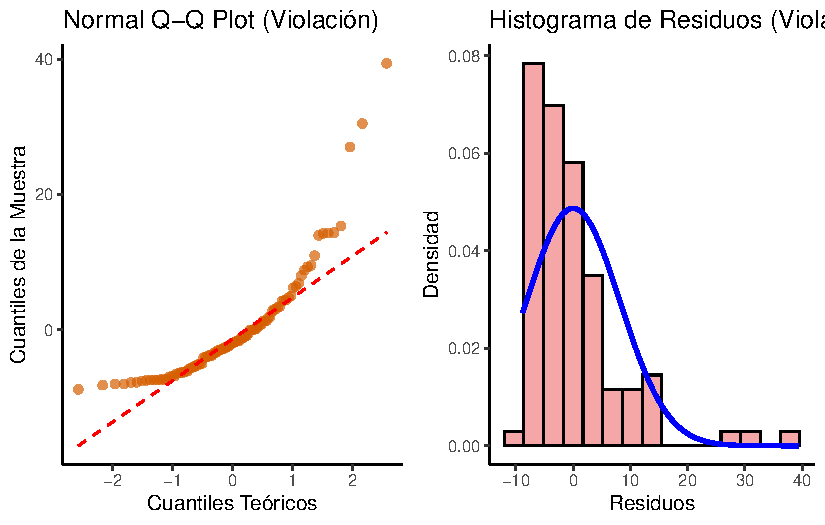
\includegraphics[keepaspectratio]{tema1_files/figure-pdf/fig-normalidad-mal-1.pdf}}

}

\caption{\label{fig-normalidad-mal}Violación del supuesto de normalidad.
Izquierda: Q-Q Plot con clara desviación. Derecha: Histograma
asimétricamente distribuido.}

\end{figure}%

La violación es evidente. En el gráfico Q-Q, los puntos se desvían
sistemáticamente de la línea diagonal, especialmente en los extremos,
formando una curva característica de distribuciones asimétricas. El
histograma muestra una clara asimetría hacia la derecha que no se ajusta
a la curva normal teórica (línea azul). La prueba de Shapiro-Wilk arroja
un \textbf{p-valor muy pequeño} (1.78e-10), rechazando fuertemente la
hipótesis nula de normalidad.

\end{tcolorbox}

\subsection{Independencia de los
residuos}\label{independencia-de-los-residuos}

Este supuesto afirma que el error de una observación no está
correlacionado con el de ninguna otra:
\(Cov(\varepsilon_i, \varepsilon_j) = 0\) para \(i \neq j\). La
violación, conocida como \textbf{autocorrelación}, es común en datos de
series temporales.

\textbf{Métodos de diagnóstico:}

\begin{enumerate}
\def\labelenumi{\arabic{enumi}.}
\item
  \textbf{Diagnóstico visual:} Gráfico de residuos vs orden de
  observación. No debe mostrar patrones temporales o secuenciales.
\item
  \textbf{Test de Durbin-Watson:} Test clásico para autocorrelación de
  primer orden.

  \begin{itemize}
  \tightlist
  \item
    \textbf{H₀:} No hay autocorrelación (\(\rho = 0\))
  \item
    \textbf{H₁:} Hay autocorrelación de orden 1
  \item
    \textbf{Estadístico:}
    \(DW = \frac{\sum_{i=2}^{n}(e_i - e_{i-1})^2}{\sum_{i=1}^{n}e_i^2}\)
  \item
    \textbf{Interpretación:} Valores cerca de 2 → no autocorrelación;
    cerca de 0 → autocorrelación positiva; cerca de 4 → autocorrelación
    negativa
  \end{itemize}
\item
  \textbf{Test de Breusch-Godfrey (LM):} Generalización del
  Durbin-Watson para órdenes superiores y regresores retardados.

  \begin{itemize}
  \tightlist
  \item
    \textbf{H₀:} No hay autocorrelación serial hasta el orden
    especificado
  \item
    \textbf{H₁:} Hay autocorrelación serial
  \item
    \textbf{Ventaja:} Más general y potente que Durbin-Watson
  \end{itemize}
\end{enumerate}

El estadístico de Durbin-Watson varía entre 0 y 4. Un valor cercano a 2
sugiere no autocorrelación. Valores cercanos a 0 indican autocorrelación
positiva, y cercanos a 4, autocorrelación negativa.

\begin{tcolorbox}[enhanced jigsaw, leftrule=.75mm, breakable, colbacktitle=quarto-callout-tip-color!10!white, bottomrule=.15mm, colframe=quarto-callout-tip-color-frame, toprule=.15mm, colback=white, coltitle=black, bottomtitle=1mm, left=2mm, title=\textcolor{quarto-callout-tip-color}{\faLightbulb}\hspace{0.5em}{Ejemplo de independencia válida}, opacityback=0, arc=.35mm, opacitybacktitle=0.6, toptitle=1mm, titlerule=0mm, rightrule=.15mm]

Para nuestro \texttt{modelo\_estudio}, evaluamos la independencia
mediante el gráfico de residuos vs orden y la prueba de Durbin-Watson.

\begin{Shaded}
\begin{Highlighting}[]
\CommentTok{\# Gráfico de residuos vs orden de observación con ggplot2}
\NormalTok{datos\_orden }\OtherTok{\textless{}{-}} \FunctionTok{data.frame}\NormalTok{(}
  \AttributeTok{orden =} \DecValTok{1}\SpecialCharTok{:}\FunctionTok{length}\NormalTok{(}\FunctionTok{residuals}\NormalTok{(modelo\_estudio)),}
  \AttributeTok{residuos =} \FunctionTok{residuals}\NormalTok{(modelo\_estudio)}
\NormalTok{)}

\FunctionTok{ggplot}\NormalTok{(datos\_orden, }\FunctionTok{aes}\NormalTok{(}\AttributeTok{x =}\NormalTok{ orden, }\AttributeTok{y =}\NormalTok{ residuos)) }\SpecialCharTok{+}
  \FunctionTok{geom\_point}\NormalTok{(}\AttributeTok{color =} \StringTok{"\#0072B2"}\NormalTok{, }\AttributeTok{alpha =} \FloatTok{0.7}\NormalTok{) }\SpecialCharTok{+}
  \FunctionTok{geom\_line}\NormalTok{(}\AttributeTok{color =} \StringTok{"\#0072B2"}\NormalTok{, }\AttributeTok{alpha =} \FloatTok{0.5}\NormalTok{) }\SpecialCharTok{+}
  \FunctionTok{geom\_hline}\NormalTok{(}\AttributeTok{yintercept =} \DecValTok{0}\NormalTok{, }\AttributeTok{color =} \StringTok{"red"}\NormalTok{, }\AttributeTok{linetype =} \StringTok{"dashed"}\NormalTok{) }\SpecialCharTok{+}
  \FunctionTok{labs}\NormalTok{(}
    \AttributeTok{title =} \StringTok{"Residuos vs Orden de Observación"}\NormalTok{,}
    \AttributeTok{x =} \StringTok{"Orden de observación"}\NormalTok{,}
    \AttributeTok{y =} \StringTok{"Residuos"}
\NormalTok{  ) }\SpecialCharTok{+}
  \FunctionTok{theme\_classic}\NormalTok{(}\AttributeTok{base\_size =} \DecValTok{12}\NormalTok{)}

\CommentTok{\# Prueba de Durbin{-}Watson}
\FunctionTok{suppressPackageStartupMessages}\NormalTok{(}\FunctionTok{library}\NormalTok{(lmtest))}
\NormalTok{dw\_resultado\_valido }\OtherTok{\textless{}{-}} \FunctionTok{dwtest}\NormalTok{(modelo\_estudio)}
\FunctionTok{print}\NormalTok{(dw\_resultado\_valido)}
\end{Highlighting}
\end{Shaded}

\begin{verbatim}

    Durbin-Watson test

data:  modelo_estudio
DW = 2.0565, p-value = 0.6104
alternative hypothesis: true autocorrelation is greater than 0
\end{verbatim}

\begin{Shaded}
\begin{Highlighting}[]
\CommentTok{\# Prueba de Breusch{-}Godfrey (más general)}
\NormalTok{bg\_resultado }\OtherTok{\textless{}{-}} \FunctionTok{bgtest}\NormalTok{(modelo\_estudio, }\AttributeTok{order =} \DecValTok{2}\NormalTok{)}
\FunctionTok{print}\NormalTok{(bg\_resultado)}
\end{Highlighting}
\end{Shaded}

\begin{verbatim}

    Breusch-Godfrey test for serial correlation of order up to 2

data:  modelo_estudio
LM test = 0.14002, df = 2, p-value = 0.9324
\end{verbatim}

\begin{figure}[H]

\centering{

\pandocbounded{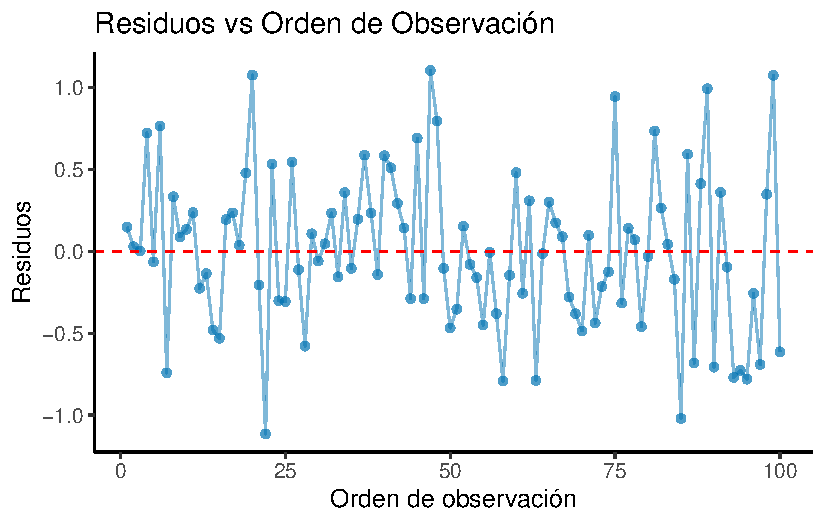
\includegraphics[keepaspectratio]{tema1_files/figure-pdf/fig-independencia-ok-1.pdf}}

}

\caption{\label{fig-independencia-ok}Diagnóstico de independencia del
modelo de estudio. Los residuos no muestran patrones temporales.}

\end{figure}%

El diagnóstico es satisfactorio. El gráfico de residuos vs orden no
muestra ningún patrón sistemático o tendencia temporal. Ambas pruebas
estadísticas confirman la independencia:

\begin{itemize}
\tightlist
\item
  \textbf{Durbin-Watson}: DW =2.056, p-valor = 0.6104 → No hay
  autocorrelación de orden 1
\item
  \textbf{Breusch-Godfrey}: LM =0.14, p-valor = 0.9324 → No hay
  autocorrelación de orden 2 fluctúan aleatoriamente alrededor del cero.
\end{itemize}

La prueba de Durbin-Watson arroja un estadístico de \textbf{2.056}
(cercano a 2) y un \textbf{p-valor de 0.61}, confirmando que no hay
evidencia de autocorrelación. \textbf{El supuesto de independencia se
cumple}.

\end{tcolorbox}

\begin{tcolorbox}[enhanced jigsaw, leftrule=.75mm, breakable, colbacktitle=quarto-callout-tip-color!10!white, bottomrule=.15mm, colframe=quarto-callout-tip-color-frame, toprule=.15mm, colback=white, coltitle=black, bottomtitle=1mm, left=2mm, title=\textcolor{quarto-callout-tip-color}{\faLightbulb}\hspace{0.5em}{Contraejemplo: Violación del supuesto de independencia}, opacityback=0, arc=.35mm, opacitybacktitle=0.6, toptitle=1mm, titlerule=0mm, rightrule=.15mm]

Simularemos datos con autocorrelación positiva, donde cada residuo está
correlacionado con el anterior, violando el supuesto de independencia.

\begin{Shaded}
\begin{Highlighting}[]
\CommentTok{\# 1. Simulación de datos con autocorrelación}
\FunctionTok{set.seed}\NormalTok{(}\DecValTok{789}\NormalTok{)}
\NormalTok{n }\OtherTok{\textless{}{-}} \DecValTok{100}
\NormalTok{x\_autocorr }\OtherTok{\textless{}{-}} \DecValTok{1}\SpecialCharTok{:}\NormalTok{n}
\CommentTok{\# Generamos errores autocorrelacionados (AR1 con phi = 0.7)}
\NormalTok{errores\_autocorr }\OtherTok{\textless{}{-}} \FunctionTok{numeric}\NormalTok{(n)}
\NormalTok{errores\_autocorr[}\DecValTok{1}\NormalTok{] }\OtherTok{\textless{}{-}} \FunctionTok{rnorm}\NormalTok{(}\DecValTok{1}\NormalTok{)}
\ControlFlowTok{for}\NormalTok{(i }\ControlFlowTok{in} \DecValTok{2}\SpecialCharTok{:}\NormalTok{n) \{}
\NormalTok{  errores\_autocorr[i] }\OtherTok{\textless{}{-}} \FloatTok{0.7} \SpecialCharTok{*}\NormalTok{ errores\_autocorr[i}\DecValTok{{-}1}\NormalTok{] }\SpecialCharTok{+} \FunctionTok{rnorm}\NormalTok{(}\DecValTok{1}\NormalTok{, }\AttributeTok{sd =} \FloatTok{0.5}\NormalTok{)}
\NormalTok{\}}

\NormalTok{y\_autocorr }\OtherTok{\textless{}{-}} \DecValTok{10} \SpecialCharTok{+} \FloatTok{1.5} \SpecialCharTok{*}\NormalTok{ x\_autocorr }\SpecialCharTok{+}\NormalTok{ errores\_autocorr }\SpecialCharTok{*} \DecValTok{3}
\NormalTok{datos\_autocorr }\OtherTok{\textless{}{-}} \FunctionTok{data.frame}\NormalTok{(}\AttributeTok{x =}\NormalTok{ x\_autocorr, }\AttributeTok{y =}\NormalTok{ y\_autocorr)}
\NormalTok{modelo\_autocorr }\OtherTok{\textless{}{-}} \FunctionTok{lm}\NormalTok{(y }\SpecialCharTok{\textasciitilde{}}\NormalTok{ x, }\AttributeTok{data =}\NormalTok{ datos\_autocorr)}

\CommentTok{\# 2. Gráfico de residuos vs orden con ggplot2}
\NormalTok{datos\_orden\_autocorr }\OtherTok{\textless{}{-}} \FunctionTok{data.frame}\NormalTok{(}
  \AttributeTok{orden =} \DecValTok{1}\SpecialCharTok{:}\FunctionTok{length}\NormalTok{(}\FunctionTok{residuals}\NormalTok{(modelo\_autocorr)),}
  \AttributeTok{residuos =} \FunctionTok{residuals}\NormalTok{(modelo\_autocorr)}
\NormalTok{)}

\FunctionTok{ggplot}\NormalTok{(datos\_orden\_autocorr, }\FunctionTok{aes}\NormalTok{(}\AttributeTok{x =}\NormalTok{ orden, }\AttributeTok{y =}\NormalTok{ residuos)) }\SpecialCharTok{+}
  \FunctionTok{geom\_point}\NormalTok{(}\AttributeTok{color =} \StringTok{"\#D55E00"}\NormalTok{, }\AttributeTok{alpha =} \FloatTok{0.7}\NormalTok{) }\SpecialCharTok{+}
  \FunctionTok{geom\_line}\NormalTok{(}\AttributeTok{color =} \StringTok{"\#D55E00"}\NormalTok{, }\AttributeTok{alpha =} \FloatTok{0.5}\NormalTok{) }\SpecialCharTok{+}
  \FunctionTok{geom\_hline}\NormalTok{(}\AttributeTok{yintercept =} \DecValTok{0}\NormalTok{, }\AttributeTok{color =} \StringTok{"blue"}\NormalTok{, }\AttributeTok{linetype =} \StringTok{"dashed"}\NormalTok{) }\SpecialCharTok{+}
  \FunctionTok{labs}\NormalTok{(}
    \AttributeTok{title =} \StringTok{"Residuos vs Orden de Observación (Violación)"}\NormalTok{,}
    \AttributeTok{x =} \StringTok{"Orden de observación"}\NormalTok{,}
    \AttributeTok{y =} \StringTok{"Residuos"}
\NormalTok{  ) }\SpecialCharTok{+}
  \FunctionTok{theme\_classic}\NormalTok{(}\AttributeTok{base\_size =} \DecValTok{12}\NormalTok{)}

\CommentTok{\# 3. Prueba de Durbin{-}Watson}
\NormalTok{dw\_resultado }\OtherTok{\textless{}{-}} \FunctionTok{dwtest}\NormalTok{(modelo\_autocorr)}
\end{Highlighting}
\end{Shaded}

\begin{figure}[H]

\centering{

\pandocbounded{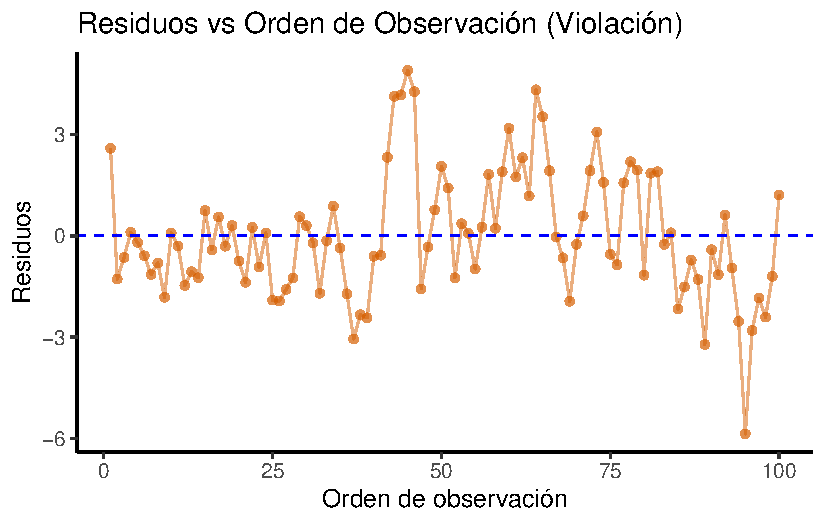
\includegraphics[keepaspectratio]{tema1_files/figure-pdf/fig-independencia-mal-1.pdf}}

}

\caption{\label{fig-independencia-mal}Violación del supuesto de
independencia. Los residuos muestran un patrón de autocorrelación
positiva.}

\end{figure}%

La violación es clara. El gráfico de residuos vs orden muestra un patrón
ondulante característico: los residuos tienden a mantenerse del mismo
signo durante varias observaciones consecutivas (rachas de valores
positivos seguidas de rachas de valores negativos). Esto indica
\textbf{autocorrelación positiva}. La prueba de Durbin-Watson confirma
esto con un estadístico muy por debajo de 2 (DW = \textbf{0.74}) y un
\textbf{p-valor muy pequeño} (\textbf{5.01e-11}), rechazando fuertemente
la hipótesis nula de independencia.

\end{tcolorbox}

\subsection{Media nula de los
residuos}\label{media-nula-de-los-residuos}

Un requisito fundamental del modelo es que la media de los residuos debe
ser exactamente cero: \(E[e_i] = 0\). Esta propiedad se deriva
matemáticamente del método de mínimos cuadrados y su verificación sirve
como una comprobación de que nuestros cálculos son correctos.

\subsection{Identificación de observaciones influyentes y
atípicas}\label{identificaciuxf3n-de-observaciones-influyentes-y-atuxedpicas}

Algunos puntos pueden tener una influencia desproporcionada en el
modelo. Es crucial identificarlos usando diferentes métricas que evalúan
aspectos complementarios de la influencia (Kutner et al. 2005; Fox and
Weisberg 2018). Las métricas desarrolladas por Cook, Belsley, Kuh y
Welsch proporcionan herramientas robustas para este diagnóstico.

\begin{tcolorbox}[enhanced jigsaw, leftrule=.75mm, breakable, colbacktitle=quarto-callout-note-color!10!white, bottomrule=.15mm, colframe=quarto-callout-note-color-frame, toprule=.15mm, colback=white, coltitle=black, bottomtitle=1mm, left=2mm, title=\textcolor{quarto-callout-note-color}{\faInfo}\hspace{0.5em}{Fundamento teórico: de los residuos simples a los estudentizados}, opacityback=0, arc=.35mm, opacitybacktitle=0.6, toptitle=1mm, titlerule=0mm, rightrule=.15mm]

Antes de analizar las métricas de influencia, debemos entender por qué
no todos los \textbf{residuos simples} (\(e_i = y_i - \hat{y}_i\)) son
comparables entre sí. El problema fundamental es que \textbf{no tienen
la misma varianza}, incluso bajo homocedasticidad.

La varianza teórica del residuo \(e_i\) depende del
\textbf{apalancamiento} (\emph{leverage}) de la observación: \[
\text{Var}(e_i) = \sigma^2(1 - h_{ii})
\]

donde el apalancamiento \(h_{ii}\) se define como: \[
h_{ii} = \frac{1}{n} + \frac{(x_i - \bar{x})^2}{\sum_{j=1}^{n}(x_j - \bar{x})^2}
\]

Las observaciones con valores de \(X\) más alejados de la media tendrán
mayor apalancamiento y, paradójicamente, residuos con \textbf{menor
varianza}. Por esto, un residuo pequeño en una observación de alto
leverage puede ser más preocupante que un residuo grande en el centro de
los datos.

\textbf{Los residuos estandarizados} solucionan parcialmente este
problema: \[
r_i^* = \frac{e_i}{\sqrt{\text{MSE}(1 - h_{ii})}}
\]

Pero \textbf{los residuos estudentizados} van un paso más allá,
eliminando el sesgo de autoinfluencia: \[
r_i = \frac{e_i}{\sqrt{\text{MSE}_{(-i)}(1 - h_{ii})}}
\]

donde \(\text{MSE}_{(-i)}\) excluye la observación \(i\) del ajuste.
Esto evita que un outlier ``contamine'' su propia evaluación y
proporciona una distribución teórica exacta (t de Student con \(n-k-2\)
grados de libertad).

\textbf{¿Por qué son superiores los residuos estudentizados?} Por tres
razones clave: (1) \textbf{eliminan el sesgo de autoinfluencia} al
excluir cada observación de su propia evaluación, (2) \textbf{evitan la
contaminación} que un outlier produce en la MSE global, y (3)
\textbf{siguen una distribución conocida} (t de Student) que permite
umbrales estadísticamente precisos. \textbf{En la práctica:}
\(|r_i| > 2\) indica posibles outliers (≈5\% en normalidad) y
\(|r_i| > 3\) outliers muy probables (\textless1\%).

\end{tcolorbox}

Las métricas fundamentales de influencia para identificar observaciones
problemáticas son:

\begin{itemize}
\item
  \textbf{Apalancamiento (Leverage,} \(h_{ii}\)): Mide cuán atípico es
  el valor de la variable predictora \(X_i\) de una observación. Un
  apalancamiento alto significa que el punto tiene el \emph{potencial}
  de ser muy influyente. En regresión simple, se calcula como:
  \[ h_{ii} = \frac{1}{n} + \frac{(x_i - \bar{x})^2}{\sum_{j=1}^{n}(x_j - \bar{x})^2} \]
  Una regla común es considerar un apalancamiento alto si
  \(h_{ii} > \frac{2(k+1)}{n}\), donde \(k\) es el número de predictores
  (1 en regresión simple).
\item
  \textbf{Distancia de Cook (}\(D_i\)): Mide la influencia global de una
  observación, combinando su apalancamiento y su residuo. Representa
  cuánto cambian los coeficientes del modelo si la i-ésima observación
  es eliminada.
  \[ D_i = \frac{r_i^2}{k+1} \cdot \frac{h_{ii}}{1-h_{ii}} \] Se
  considera que un punto es influyente si su distancia de Cook es
  grande, por ejemplo, si \(D_i > 1\) o \(D_i > 4/(n-k-1)\).
\item
  \textbf{DFFITS:} Mide cuánto cambia la predicción \(\hat{y}_i\) cuando
  se elimina la i-ésima observación. Es una medida estandarizada que
  combina el residuo estudentizado y el apalancamiento.
  \[ \text{DFFITS}_i = r_i \sqrt{\frac{h_{ii}}{1-h_{ii}}} \] Un punto se
  considera influyente si \(|\text{DFFITS}_i| > 2\sqrt{(k+1)/n}\), donde
  \(k\) es el número de predictores.
\end{itemize}

\begin{tcolorbox}[enhanced jigsaw, leftrule=.75mm, breakable, colbacktitle=quarto-callout-tip-color!10!white, bottomrule=.15mm, colframe=quarto-callout-tip-color-frame, toprule=.15mm, colback=white, coltitle=black, bottomtitle=1mm, left=2mm, title=\textcolor{quarto-callout-tip-color}{\faLightbulb}\hspace{0.5em}{Ejemplo: Cálculo y análisis de DFFITS}, opacityback=0, arc=.35mm, opacitybacktitle=0.6, toptitle=1mm, titlerule=0mm, rightrule=.15mm]

DFFITS es especialmente útil para evaluar cómo cada observación afecta a
su propia predicción. Analicemos esta medida con nuestro
\texttt{modelo\_estudio}.

\begin{Shaded}
\begin{Highlighting}[]
\CommentTok{\# Calcular DFFITS y sus componentes}
\NormalTok{dffits\_vals }\OtherTok{\textless{}{-}} \FunctionTok{dffits}\NormalTok{(modelo\_estudio)}
\NormalTok{residuos\_stud }\OtherTok{\textless{}{-}} \FunctionTok{rstudent}\NormalTok{(modelo\_estudio)  }\CommentTok{\# Residuos estudentizados}
\NormalTok{leverage\_vals }\OtherTok{\textless{}{-}} \FunctionTok{hatvalues}\NormalTok{(modelo\_estudio)}

\CommentTok{\# Crear dataframe para análisis}
\NormalTok{datos\_dffits }\OtherTok{\textless{}{-}} \FunctionTok{data.frame}\NormalTok{(}
  \AttributeTok{observacion =} \DecValTok{1}\SpecialCharTok{:}\FunctionTok{length}\NormalTok{(dffits\_vals),}
  \AttributeTok{dffits =}\NormalTok{ dffits\_vals,}
  \AttributeTok{residuo\_stud =}\NormalTok{ residuos\_stud,}
  \AttributeTok{leverage =}\NormalTok{ leverage\_vals}
\NormalTok{)}

\CommentTok{\# Umbral de DFFITS}
\NormalTok{n }\OtherTok{\textless{}{-}} \FunctionTok{nrow}\NormalTok{(datos)}
\NormalTok{k }\OtherTok{\textless{}{-}} \DecValTok{1}  \CommentTok{\# número de predictores}
\NormalTok{dffits\_threshold }\OtherTok{\textless{}{-}} \DecValTok{2} \SpecialCharTok{*} \FunctionTok{sqrt}\NormalTok{((k }\SpecialCharTok{+} \DecValTok{1}\NormalTok{) }\SpecialCharTok{/}\NormalTok{ n)}

\CommentTok{\# Gráfico de DFFITS}
\FunctionTok{ggplot}\NormalTok{(datos\_dffits, }\FunctionTok{aes}\NormalTok{(}\AttributeTok{x =}\NormalTok{ observacion, }\AttributeTok{y =}\NormalTok{ dffits)) }\SpecialCharTok{+}
  \FunctionTok{geom\_point}\NormalTok{(}\AttributeTok{color =} \StringTok{"\#0072B2"}\NormalTok{, }\AttributeTok{alpha =} \FloatTok{0.7}\NormalTok{) }\SpecialCharTok{+}
  \FunctionTok{geom\_hline}\NormalTok{(}\AttributeTok{yintercept =} \DecValTok{0}\NormalTok{, }\AttributeTok{color =} \StringTok{"gray"}\NormalTok{, }\AttributeTok{linetype =} \StringTok{"dashed"}\NormalTok{) }\SpecialCharTok{+}
  \FunctionTok{geom\_hline}\NormalTok{(}\AttributeTok{yintercept =} \FunctionTok{c}\NormalTok{(}\SpecialCharTok{{-}}\NormalTok{dffits\_threshold, dffits\_threshold), }
             \AttributeTok{color =} \StringTok{"red"}\NormalTok{, }\AttributeTok{linetype =} \StringTok{"dashed"}\NormalTok{, }\AttributeTok{alpha =} \FloatTok{0.7}\NormalTok{) }\SpecialCharTok{+}
  \FunctionTok{labs}\NormalTok{(}
    \AttributeTok{title =} \StringTok{"DFFITS por Observación"}\NormalTok{,}
    \AttributeTok{x =} \StringTok{"Número de Observación"}\NormalTok{,}
    \AttributeTok{y =} \StringTok{"DFFITS"}\NormalTok{,}
    \AttributeTok{caption =} \FunctionTok{paste}\NormalTok{(}\StringTok{"Líneas rojas: umbrales ±"}\NormalTok{, }\FunctionTok{round}\NormalTok{(dffits\_threshold, }\DecValTok{3}\NormalTok{))}
\NormalTok{  ) }\SpecialCharTok{+}
  \FunctionTok{theme\_classic}\NormalTok{(}\AttributeTok{base\_size =} \DecValTok{12}\NormalTok{)}

\CommentTok{\# Análisis cuantitativo}
\NormalTok{influential\_dffits }\OtherTok{\textless{}{-}} \FunctionTok{which}\NormalTok{(}\FunctionTok{abs}\NormalTok{(dffits\_vals) }\SpecialCharTok{\textgreater{}}\NormalTok{ dffits\_threshold)}
\NormalTok{top\_indices }\OtherTok{\textless{}{-}} \FunctionTok{order}\NormalTok{(}\FunctionTok{abs}\NormalTok{(dffits\_vals), }\AttributeTok{decreasing =} \ConstantTok{TRUE}\NormalTok{)[}\DecValTok{1}\SpecialCharTok{:}\DecValTok{5}\NormalTok{]}
\end{Highlighting}
\end{Shaded}

\begin{figure}[H]

\centering{

\pandocbounded{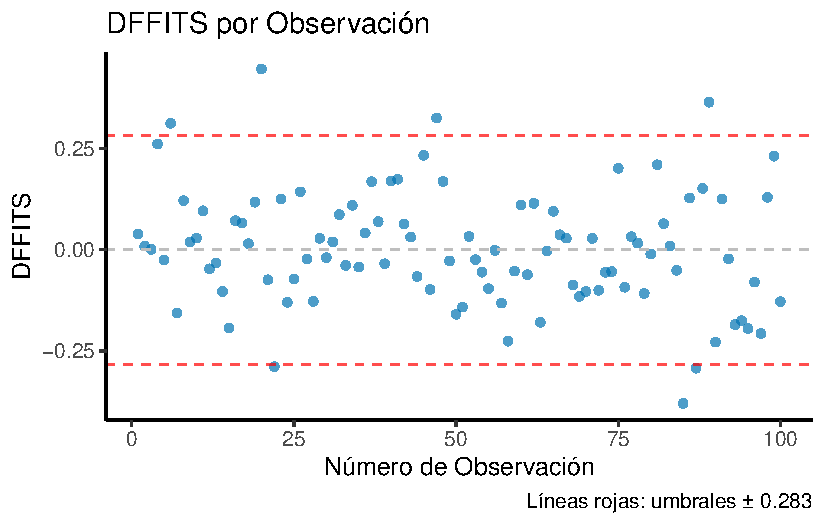
\includegraphics[keepaspectratio]{tema1_files/figure-pdf/fig-dffits-1.pdf}}

}

\caption{\label{fig-dffits}Análisis de DFFITS para identificar
observaciones que afectan significativamente a sus propias
predicciones.}

\end{figure}%

\textbf{Análisis de resultados:}

El umbral de influencia para DFFITS es 0.283. En nuestro modelo,
\textbf{7 observaciones superan este umbral}: las observaciones 6, 20,
22, 47, 85, 87, 89, lo que las clasifica como influyentes según este
criterio.

Las \textbf{cinco observaciones con mayor \textbar DFFITS\textbar{}} son
las observaciones 20, 85, 89, 47, 6, con valores de 0.446, -0.38, 0.364,
0.325, 0.312 respectivamente. Lo más notable es que \textbf{todas estas
cinco observaciones} (20, 85, 89, 47, 6) \textbf{superan el umbral de
DFFITS}, confirmando su carácter influyente.

\textbf{Interpretación clave:} La observación 20 es el caso más
destacado: tiene un DFFITS de 0.446, superando el umbral de 0.283. Esta
combinación de residuo y apalancamiento resulta en un DFFITS
significativo que indica cambios sustanciales en su predicción.

\textbf{Conclusión práctica:} Tenemos \textbf{7 observaciones
influyentes} según DFFITS (6, 20, 22, 47, 85, 87, 89) que merecen
investigación adicional. Estas observaciones cambian significativamente
sus propias predicciones cuando son eliminadas del modelo, sugiriendo
que podrían representar casos especiales o errores de medición que
deberían ser examinados más detalladamente.

\end{tcolorbox}

El gráfico \textbf{\texttt{Residuals\ vs.\ Leverage}} es la herramienta
visual más importante para el diagnóstico de influencia, ya que combina
en un solo gráfico el \textbf{apalancamiento} (eje X) y los
\textbf{residuos estudentizados} (eje Y), permitiendo identificar
simultáneamente observaciones con alto leverage y outliers. Además,
incluye curvas que delimitan regiones de alta \textbf{Distancia de
Cook}, facilitando la identificación visual de los puntos más
problemáticos.

\begin{tcolorbox}[enhanced jigsaw, leftrule=.75mm, breakable, colbacktitle=quarto-callout-tip-color!10!white, bottomrule=.15mm, colframe=quarto-callout-tip-color-frame, toprule=.15mm, colback=white, coltitle=black, bottomtitle=1mm, left=2mm, title=\textcolor{quarto-callout-tip-color}{\faLightbulb}\hspace{0.5em}{Ejemplo: Gráfico Residuals vs.~Leverage}, opacityback=0, arc=.35mm, opacitybacktitle=0.6, toptitle=1mm, titlerule=0mm, rightrule=.15mm]

Vamos a analizar el gráfico más importante para el diagnóstico de
influencia usando nuestro \texttt{modelo\_estudio}.

\begin{Shaded}
\begin{Highlighting}[]
\CommentTok{\# Crear datos para el gráfico Residuals vs. Leverage}
\NormalTok{leverage\_vals }\OtherTok{\textless{}{-}} \FunctionTok{hatvalues}\NormalTok{(modelo\_estudio)}
\NormalTok{residuos\_stud }\OtherTok{\textless{}{-}} \FunctionTok{rstudent}\NormalTok{(modelo\_estudio)  }\CommentTok{\# Residuos estudentizados}
\NormalTok{cook\_dist }\OtherTok{\textless{}{-}} \FunctionTok{cooks.distance}\NormalTok{(modelo\_estudio)}

\NormalTok{datos\_leverage }\OtherTok{\textless{}{-}} \FunctionTok{data.frame}\NormalTok{(}
  \AttributeTok{leverage =}\NormalTok{ leverage\_vals,}
  \AttributeTok{residuos\_stud =}\NormalTok{ residuos\_stud,}
  \AttributeTok{cook =}\NormalTok{ cook\_dist,}
  \AttributeTok{observacion =} \DecValTok{1}\SpecialCharTok{:}\FunctionTok{length}\NormalTok{(leverage\_vals)}
\NormalTok{)}

\CommentTok{\# Calcular umbrales}
\NormalTok{n }\OtherTok{\textless{}{-}} \FunctionTok{nrow}\NormalTok{(datos)}
\NormalTok{k }\OtherTok{\textless{}{-}} \DecValTok{1}
\NormalTok{leverage\_threshold }\OtherTok{\textless{}{-}} \DecValTok{2} \SpecialCharTok{*}\NormalTok{ (k }\SpecialCharTok{+} \DecValTok{1}\NormalTok{) }\SpecialCharTok{/}\NormalTok{ n}
\NormalTok{cook\_threshold }\OtherTok{\textless{}{-}} \DecValTok{4} \SpecialCharTok{/}\NormalTok{ (n }\SpecialCharTok{{-}}\NormalTok{ k }\SpecialCharTok{{-}} \DecValTok{1}\NormalTok{)}

\CommentTok{\# Función para crear curvas de Cook}
\NormalTok{cook\_curve }\OtherTok{\textless{}{-}} \ControlFlowTok{function}\NormalTok{(leverage, cook\_value, k) \{}
  \FunctionTok{sqrt}\NormalTok{(cook\_value }\SpecialCharTok{*}\NormalTok{ (k }\SpecialCharTok{+} \DecValTok{1}\NormalTok{) }\SpecialCharTok{*}\NormalTok{ (}\DecValTok{1} \SpecialCharTok{{-}}\NormalTok{ leverage) }\SpecialCharTok{/}\NormalTok{ leverage)}
\NormalTok{\}}

\CommentTok{\# Crear curvas de Cook para diferentes valores}
\NormalTok{lev\_seq }\OtherTok{\textless{}{-}} \FunctionTok{seq}\NormalTok{(}\FloatTok{0.001}\NormalTok{, }\FunctionTok{max}\NormalTok{(leverage\_vals) }\SpecialCharTok{*} \FloatTok{1.1}\NormalTok{, }\AttributeTok{length.out =} \DecValTok{100}\NormalTok{)}
\NormalTok{cook\_05 }\OtherTok{\textless{}{-}} \FunctionTok{data.frame}\NormalTok{(}
  \AttributeTok{leverage =}\NormalTok{ lev\_seq,}
  \AttributeTok{pos =} \FunctionTok{cook\_curve}\NormalTok{(lev\_seq, }\FloatTok{0.5}\NormalTok{, k),}
  \AttributeTok{neg =} \SpecialCharTok{{-}}\FunctionTok{cook\_curve}\NormalTok{(lev\_seq, }\FloatTok{0.5}\NormalTok{, k)}
\NormalTok{)}
\NormalTok{cook\_1 }\OtherTok{\textless{}{-}} \FunctionTok{data.frame}\NormalTok{(}
  \AttributeTok{leverage =}\NormalTok{ lev\_seq,}
  \AttributeTok{pos =} \FunctionTok{cook\_curve}\NormalTok{(lev\_seq, }\DecValTok{1}\NormalTok{, k),}
  \AttributeTok{neg =} \SpecialCharTok{{-}}\FunctionTok{cook\_curve}\NormalTok{(lev\_seq, }\DecValTok{1}\NormalTok{, k)}
\NormalTok{)}

\CommentTok{\# Gráfico Residuals vs. Leverage con ggplot2}
\FunctionTok{ggplot}\NormalTok{(datos\_leverage, }\FunctionTok{aes}\NormalTok{(}\AttributeTok{x =}\NormalTok{ leverage, }\AttributeTok{y =}\NormalTok{ residuos\_stud)) }\SpecialCharTok{+}
  \CommentTok{\# Curvas de Cook}
  \FunctionTok{geom\_line}\NormalTok{(}\AttributeTok{data =}\NormalTok{ cook\_05, }\FunctionTok{aes}\NormalTok{(}\AttributeTok{x =}\NormalTok{ leverage, }\AttributeTok{y =}\NormalTok{ pos), }
            \AttributeTok{color =} \StringTok{"red"}\NormalTok{, }\AttributeTok{linetype =} \StringTok{"dashed"}\NormalTok{, }\AttributeTok{alpha =} \FloatTok{0.6}\NormalTok{, }\AttributeTok{inherit.aes =} \ConstantTok{FALSE}\NormalTok{) }\SpecialCharTok{+}
  \FunctionTok{geom\_line}\NormalTok{(}\AttributeTok{data =}\NormalTok{ cook\_05, }\FunctionTok{aes}\NormalTok{(}\AttributeTok{x =}\NormalTok{ leverage, }\AttributeTok{y =}\NormalTok{ neg), }
            \AttributeTok{color =} \StringTok{"red"}\NormalTok{, }\AttributeTok{linetype =} \StringTok{"dashed"}\NormalTok{, }\AttributeTok{alpha =} \FloatTok{0.6}\NormalTok{, }\AttributeTok{inherit.aes =} \ConstantTok{FALSE}\NormalTok{) }\SpecialCharTok{+}
  \FunctionTok{geom\_line}\NormalTok{(}\AttributeTok{data =}\NormalTok{ cook\_1, }\FunctionTok{aes}\NormalTok{(}\AttributeTok{x =}\NormalTok{ leverage, }\AttributeTok{y =}\NormalTok{ pos), }
            \AttributeTok{color =} \StringTok{"red"}\NormalTok{, }\AttributeTok{linetype =} \StringTok{"solid"}\NormalTok{, }\AttributeTok{alpha =} \FloatTok{0.8}\NormalTok{, }\AttributeTok{inherit.aes =} \ConstantTok{FALSE}\NormalTok{) }\SpecialCharTok{+}
  \FunctionTok{geom\_line}\NormalTok{(}\AttributeTok{data =}\NormalTok{ cook\_1, }\FunctionTok{aes}\NormalTok{(}\AttributeTok{x =}\NormalTok{ leverage, }\AttributeTok{y =}\NormalTok{ neg), }
            \AttributeTok{color =} \StringTok{"red"}\NormalTok{, }\AttributeTok{linetype =} \StringTok{"solid"}\NormalTok{, }\AttributeTok{alpha =} \FloatTok{0.8}\NormalTok{, }\AttributeTok{inherit.aes =} \ConstantTok{FALSE}\NormalTok{) }\SpecialCharTok{+}
  \CommentTok{\# Puntos de datos}
  \FunctionTok{geom\_point}\NormalTok{(}\AttributeTok{color =} \StringTok{"\#0072B2"}\NormalTok{, }\AttributeTok{alpha =} \FloatTok{0.7}\NormalTok{, }\AttributeTok{size =} \DecValTok{2}\NormalTok{) }\SpecialCharTok{+}
  \CommentTok{\# Líneas de referencia}
  \FunctionTok{geom\_hline}\NormalTok{(}\AttributeTok{yintercept =} \DecValTok{0}\NormalTok{, }\AttributeTok{color =} \StringTok{"gray"}\NormalTok{, }\AttributeTok{linetype =} \StringTok{"dashed"}\NormalTok{) }\SpecialCharTok{+}
  \FunctionTok{geom\_hline}\NormalTok{(}\AttributeTok{yintercept =} \FunctionTok{c}\NormalTok{(}\SpecialCharTok{{-}}\DecValTok{2}\NormalTok{, }\DecValTok{2}\NormalTok{), }\AttributeTok{color =} \StringTok{"orange"}\NormalTok{, }\AttributeTok{linetype =} \StringTok{"dotted"}\NormalTok{, }\AttributeTok{alpha =} \FloatTok{0.7}\NormalTok{) }\SpecialCharTok{+}
  \FunctionTok{geom\_vline}\NormalTok{(}\AttributeTok{xintercept =}\NormalTok{ leverage\_threshold, }\AttributeTok{color =} \StringTok{"purple"}\NormalTok{, }\AttributeTok{linetype =} \StringTok{"dotted"}\NormalTok{, }\AttributeTok{alpha =} \FloatTok{0.7}\NormalTok{) }\SpecialCharTok{+}
  \CommentTok{\# Etiquetas}
  \FunctionTok{labs}\NormalTok{(}
    \AttributeTok{title =} \StringTok{"Residuals vs. Leverage"}\NormalTok{,}
    \AttributeTok{x =} \StringTok{"Leverage"}\NormalTok{,}
    \AttributeTok{y =} \StringTok{"Residuos Estudentizados"}\NormalTok{,}
    \AttributeTok{caption =} \StringTok{"Curvas rojas: Cook 0.5 (discontinua) y 1.0 (continua) | Líneas naranjas: ±2 | Línea morada: umbral leverage"}
\NormalTok{  ) }\SpecialCharTok{+}
  \FunctionTok{theme\_classic}\NormalTok{(}\AttributeTok{base\_size =} \DecValTok{12}\NormalTok{)}

\CommentTok{\# Identificar observaciones problemáticas}
\NormalTok{high\_leverage }\OtherTok{\textless{}{-}} \FunctionTok{which}\NormalTok{(leverage\_vals }\SpecialCharTok{\textgreater{}}\NormalTok{ leverage\_threshold)}
\NormalTok{outliers\_stud }\OtherTok{\textless{}{-}} \FunctionTok{which}\NormalTok{(}\FunctionTok{abs}\NormalTok{(residuos\_stud) }\SpecialCharTok{\textgreater{}} \DecValTok{2}\NormalTok{)}
\NormalTok{high\_cook }\OtherTok{\textless{}{-}} \FunctionTok{which}\NormalTok{(cook\_dist }\SpecialCharTok{\textgreater{}}\NormalTok{ cook\_threshold)}
\end{Highlighting}
\end{Shaded}

\begin{figure}[H]

\centering{

\pandocbounded{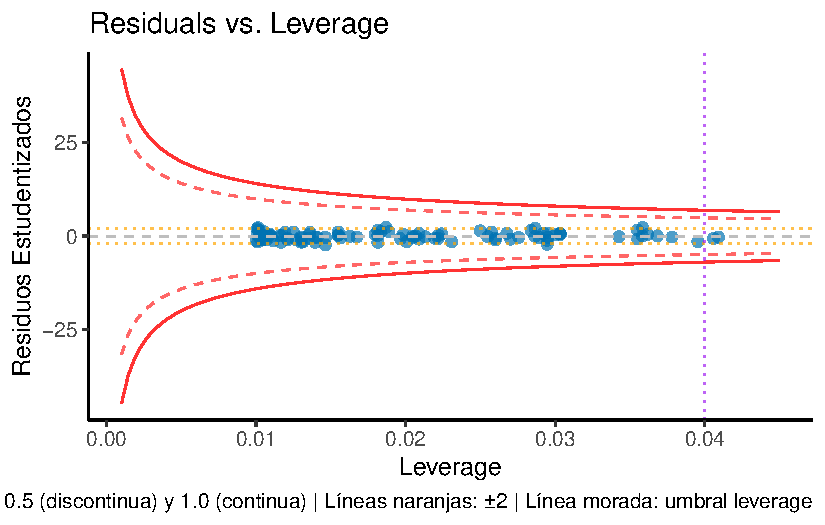
\includegraphics[keepaspectratio]{tema1_files/figure-pdf/fig-leverage-1.pdf}}

}

\caption{\label{fig-leverage}Gráfico Residuals vs.~Leverage para
identificar observaciones influyentes.}

\end{figure}%

\textbf{Análisis del gráfico:}

El gráfico revela varios puntos importantes. Tenemos 6 outliers
(residuos estudentizados \textgreater{} 2): las observaciones 20, 22,
47, 85, 89, 99. Además, 2 observaciones superan el umbral de leverage
(\textgreater{} 0.04): las observaciones 24, 74.

\textbf{Interpretación por regiones:}

\begin{itemize}
\tightlist
\item
  \textbf{Zona derecha (alto leverage)}: Las observaciones 24, 74
  superan el umbral de leverage, lo que significa que tienen valores de
  X atípicos y \textbf{alto potencial influyente}
\item
  \textbf{Zona izquierda superior/inferior}: Los 6 outliers (20, 22, 47,
  85, 89, 99) están distribuidos aquí, con leverage bajo-moderado pero
  residuos grandes
\item
  \textbf{Esquinas críticas}: Afortunadamente vacías (alto leverage +
  outlier sería muy problemático)
\end{itemize}

\textbf{Distancia de Cook:} Las curvas rojas muestran que aunque ningún
punto supera Cook = 1.0 (línea continua), \textbf{varios puntos se
acercan a la curva de Cook = 0.5} (línea discontinua), indicando
influencia moderada. Las observaciones con alto leverage están en esta
zona de influencia moderada.

\textbf{Conclusión práctica:} El modelo presenta una \textbf{situación
favorable}: aunque tenemos \textbf{outliers} (observaciones 20, 22, 47,
85, 89, 99) que son atípicos en Y, y \textbf{observaciones de alto
leverage} (observaciones 24, 74) que son atípicos en X,
\textbf{crucialmente no hay solapamiento entre ambos grupos}. Esto
significa que no tenemos la situación más problemática (alto leverage +
outlier). Aun así, ambos grupos merecen investigación.

\end{tcolorbox}

\subsubsection{Interpretación práctica de las medidas de
influencia}\label{interpretaciuxf3n-pruxe1ctica-de-las-medidas-de-influencia}

Cada medida nos proporciona información complementaria sobre diferentes
aspectos de la influencia:

\begin{itemize}
\item
  \textbf{Leverage (Apalancamiento):} Identifica observaciones con
  valores ``raros'' en las variables predictoras. Alto leverage no es
  necesariamente problemático, pero indica potencial para ser
  influyente.
\item
  \textbf{Distancia de Cook:} Es la medida más general de influencia.
  Valores altos indican que eliminar esa observación cambiaría
  substancialmente los coeficientes del modelo.
\item
  \textbf{DFFITS:} Se enfoca específicamente en cómo cambia la
  predicción de cada punto cuando se elimina esa observación. Es
  especialmente útil para evaluar el impacto en las predicciones.
\end{itemize}

En la práctica, una observación es especialmente preocupante si es
problemática según \textbf{múltiples criterios} a la vez.

\begin{tcolorbox}[enhanced jigsaw, leftrule=.75mm, breakable, colbacktitle=quarto-callout-tip-color!10!white, bottomrule=.15mm, colframe=quarto-callout-tip-color-frame, toprule=.15mm, colback=white, coltitle=black, bottomtitle=1mm, left=2mm, title=\textcolor{quarto-callout-tip-color}{\faLightbulb}\hspace{0.5em}{Diagnóstico completo del modelo de estudio}, opacityback=0, arc=.35mm, opacitybacktitle=0.6, toptitle=1mm, titlerule=0mm, rightrule=.15mm]

A continuación, realizamos todas las verificaciones de diagnóstico para
nuestro \texttt{modelo\_estudio}:

\begin{Shaded}
\begin{Highlighting}[]
\CommentTok{\# Preparar todos los datos necesarios para los gráficos}
\NormalTok{residuos\_completo }\OtherTok{\textless{}{-}} \FunctionTok{residuals}\NormalTok{(modelo\_estudio)}
\NormalTok{valores\_ajustados\_completo }\OtherTok{\textless{}{-}} \FunctionTok{fitted}\NormalTok{(modelo\_estudio)}
\NormalTok{residuos\_std }\OtherTok{\textless{}{-}} \FunctionTok{rstandard}\NormalTok{(modelo\_estudio)}
\NormalTok{leverage\_vals }\OtherTok{\textless{}{-}} \FunctionTok{hatvalues}\NormalTok{(modelo\_estudio)}

\CommentTok{\# 1. Gráfico Residuos vs. Valores Ajustados}
\NormalTok{p1\_completo }\OtherTok{\textless{}{-}} \FunctionTok{ggplot}\NormalTok{(}\FunctionTok{data.frame}\NormalTok{(}\AttributeTok{x =}\NormalTok{ valores\_ajustados\_completo, }\AttributeTok{y =}\NormalTok{ residuos\_completo), }
                      \FunctionTok{aes}\NormalTok{(}\AttributeTok{x =}\NormalTok{ x, }\AttributeTok{y =}\NormalTok{ y)) }\SpecialCharTok{+}
  \FunctionTok{geom\_point}\NormalTok{(}\AttributeTok{color =} \StringTok{"\#0072B2"}\NormalTok{, }\AttributeTok{alpha =} \FloatTok{0.7}\NormalTok{) }\SpecialCharTok{+}
  \FunctionTok{geom\_hline}\NormalTok{(}\AttributeTok{yintercept =} \DecValTok{0}\NormalTok{, }\AttributeTok{color =} \StringTok{"red"}\NormalTok{, }\AttributeTok{linetype =} \StringTok{"dashed"}\NormalTok{) }\SpecialCharTok{+}
  \FunctionTok{geom\_smooth}\NormalTok{(}\AttributeTok{method =} \StringTok{"loess"}\NormalTok{, }\AttributeTok{se =} \ConstantTok{FALSE}\NormalTok{, }\AttributeTok{color =} \StringTok{"red"}\NormalTok{, }\AttributeTok{linewidth =} \FloatTok{0.8}\NormalTok{, }\AttributeTok{formula =}\NormalTok{ y }\SpecialCharTok{\textasciitilde{}}\NormalTok{ x) }\SpecialCharTok{+}
  \FunctionTok{labs}\NormalTok{(}\AttributeTok{title =} \StringTok{"Residuos vs. Valores Ajustados"}\NormalTok{, }\AttributeTok{x =} \StringTok{"Valores Ajustados"}\NormalTok{, }\AttributeTok{y =} \StringTok{"Residuos"}\NormalTok{) }\SpecialCharTok{+}
  \FunctionTok{theme\_classic}\NormalTok{(}\AttributeTok{base\_size =} \DecValTok{10}\NormalTok{)}

\CommentTok{\# 2. Gráfico Q{-}Q Normal}
\NormalTok{datos\_qq\_completo }\OtherTok{\textless{}{-}} \FunctionTok{data.frame}\NormalTok{(}\AttributeTok{residuos =}\NormalTok{ residuos\_std)}

\NormalTok{p2\_completo }\OtherTok{\textless{}{-}} \FunctionTok{ggplot}\NormalTok{(datos\_qq\_completo, }\FunctionTok{aes}\NormalTok{(}\AttributeTok{sample =}\NormalTok{ residuos)) }\SpecialCharTok{+}
  \FunctionTok{geom\_qq}\NormalTok{(}\AttributeTok{color =} \StringTok{"\#0072B2"}\NormalTok{, }\AttributeTok{alpha =} \FloatTok{0.7}\NormalTok{) }\SpecialCharTok{+}
  \FunctionTok{geom\_qq\_line}\NormalTok{(}\AttributeTok{color =} \StringTok{"red"}\NormalTok{, }\AttributeTok{linetype =} \StringTok{"dashed"}\NormalTok{) }\SpecialCharTok{+}
  \FunctionTok{labs}\NormalTok{(}\AttributeTok{title =} \StringTok{"Normal Q{-}Q Plot"}\NormalTok{, }\AttributeTok{x =} \StringTok{"Cuantiles Teóricos"}\NormalTok{, }\AttributeTok{y =} \StringTok{"Cuantiles de la Muestra"}\NormalTok{) }\SpecialCharTok{+}
  \FunctionTok{theme\_classic}\NormalTok{(}\AttributeTok{base\_size =} \DecValTok{10}\NormalTok{)}

\CommentTok{\# 3. Gráfico Scale{-}Location}
\NormalTok{p3\_completo }\OtherTok{\textless{}{-}} \FunctionTok{ggplot}\NormalTok{(}\FunctionTok{data.frame}\NormalTok{(}\AttributeTok{x =}\NormalTok{ valores\_ajustados\_completo, }
                                 \AttributeTok{y =} \FunctionTok{sqrt}\NormalTok{(}\FunctionTok{abs}\NormalTok{(residuos\_std))), }
                      \FunctionTok{aes}\NormalTok{(}\AttributeTok{x =}\NormalTok{ x, }\AttributeTok{y =}\NormalTok{ y)) }\SpecialCharTok{+}
  \FunctionTok{geom\_point}\NormalTok{(}\AttributeTok{color =} \StringTok{"\#0072B2"}\NormalTok{, }\AttributeTok{alpha =} \FloatTok{0.7}\NormalTok{) }\SpecialCharTok{+}
  \FunctionTok{geom\_smooth}\NormalTok{(}\AttributeTok{method =} \StringTok{"loess"}\NormalTok{, }\AttributeTok{se =} \ConstantTok{FALSE}\NormalTok{, }\AttributeTok{color =} \StringTok{"red"}\NormalTok{, }\AttributeTok{linewidth =} \FloatTok{0.8}\NormalTok{, }\AttributeTok{formula =}\NormalTok{ y }\SpecialCharTok{\textasciitilde{}}\NormalTok{ x) }\SpecialCharTok{+}
  \FunctionTok{labs}\NormalTok{(}\AttributeTok{title =} \StringTok{"Scale{-}Location"}\NormalTok{, }\AttributeTok{x =} \StringTok{"Valores Ajustados"}\NormalTok{, }
       \AttributeTok{y =} \FunctionTok{expression}\NormalTok{(}\FunctionTok{sqrt}\NormalTok{(}\StringTok{"|Residuos Estandarizados|"}\NormalTok{))) }\SpecialCharTok{+}
  \FunctionTok{theme\_classic}\NormalTok{(}\AttributeTok{base\_size =} \DecValTok{10}\NormalTok{)}

\CommentTok{\# 4. Gráfico Residuos vs. Leverage (con curvas de Cook)}
\NormalTok{p4\_completo }\OtherTok{\textless{}{-}} \FunctionTok{ggplot}\NormalTok{(datos\_leverage, }\FunctionTok{aes}\NormalTok{(}\AttributeTok{x =}\NormalTok{ leverage, }\AttributeTok{y =}\NormalTok{ residuos\_stud)) }\SpecialCharTok{+}
  \CommentTok{\# Curvas de Cook}
  \FunctionTok{geom\_line}\NormalTok{(}\AttributeTok{data =}\NormalTok{ cook\_05, }\FunctionTok{aes}\NormalTok{(}\AttributeTok{x =}\NormalTok{ leverage, }\AttributeTok{y =}\NormalTok{ pos), }
            \AttributeTok{color =} \StringTok{"red"}\NormalTok{, }\AttributeTok{linetype =} \StringTok{"dashed"}\NormalTok{, }\AttributeTok{alpha =} \FloatTok{0.6}\NormalTok{, }\AttributeTok{inherit.aes =} \ConstantTok{FALSE}\NormalTok{) }\SpecialCharTok{+}
  \FunctionTok{geom\_line}\NormalTok{(}\AttributeTok{data =}\NormalTok{ cook\_05, }\FunctionTok{aes}\NormalTok{(}\AttributeTok{x =}\NormalTok{ leverage, }\AttributeTok{y =}\NormalTok{ neg), }
            \AttributeTok{color =} \StringTok{"red"}\NormalTok{, }\AttributeTok{linetype =} \StringTok{"dashed"}\NormalTok{, }\AttributeTok{alpha =} \FloatTok{0.6}\NormalTok{, }\AttributeTok{inherit.aes =} \ConstantTok{FALSE}\NormalTok{) }\SpecialCharTok{+}
  \FunctionTok{geom\_line}\NormalTok{(}\AttributeTok{data =}\NormalTok{ cook\_1, }\FunctionTok{aes}\NormalTok{(}\AttributeTok{x =}\NormalTok{ leverage, }\AttributeTok{y =}\NormalTok{ pos), }
            \AttributeTok{color =} \StringTok{"red"}\NormalTok{, }\AttributeTok{linetype =} \StringTok{"solid"}\NormalTok{, }\AttributeTok{alpha =} \FloatTok{0.8}\NormalTok{, }\AttributeTok{inherit.aes =} \ConstantTok{FALSE}\NormalTok{) }\SpecialCharTok{+}
  \FunctionTok{geom\_line}\NormalTok{(}\AttributeTok{data =}\NormalTok{ cook\_1, }\FunctionTok{aes}\NormalTok{(}\AttributeTok{x =}\NormalTok{ leverage, }\AttributeTok{y =}\NormalTok{ neg), }
            \AttributeTok{color =} \StringTok{"red"}\NormalTok{, }\AttributeTok{linetype =} \StringTok{"solid"}\NormalTok{, }\AttributeTok{alpha =} \FloatTok{0.8}\NormalTok{, }\AttributeTok{inherit.aes =} \ConstantTok{FALSE}\NormalTok{) }\SpecialCharTok{+}
  \CommentTok{\# Puntos de datos}
  \FunctionTok{geom\_point}\NormalTok{(}\AttributeTok{color =} \StringTok{"\#0072B2"}\NormalTok{, }\AttributeTok{alpha =} \FloatTok{0.7}\NormalTok{, }\AttributeTok{size =} \FloatTok{1.5}\NormalTok{) }\SpecialCharTok{+}
  \CommentTok{\# Líneas de referencia}
  \FunctionTok{geom\_hline}\NormalTok{(}\AttributeTok{yintercept =} \DecValTok{0}\NormalTok{, }\AttributeTok{color =} \StringTok{"gray"}\NormalTok{, }\AttributeTok{linetype =} \StringTok{"dashed"}\NormalTok{) }\SpecialCharTok{+}
  \FunctionTok{geom\_hline}\NormalTok{(}\AttributeTok{yintercept =} \FunctionTok{c}\NormalTok{(}\SpecialCharTok{{-}}\DecValTok{2}\NormalTok{, }\DecValTok{2}\NormalTok{), }\AttributeTok{color =} \StringTok{"orange"}\NormalTok{, }\AttributeTok{linetype =} \StringTok{"dotted"}\NormalTok{, }\AttributeTok{alpha =} \FloatTok{0.7}\NormalTok{) }\SpecialCharTok{+}
  \FunctionTok{geom\_vline}\NormalTok{(}\AttributeTok{xintercept =}\NormalTok{ leverage\_threshold, }\AttributeTok{color =} \StringTok{"purple"}\NormalTok{, }\AttributeTok{linetype =} \StringTok{"dotted"}\NormalTok{, }\AttributeTok{alpha =} \FloatTok{0.7}\NormalTok{) }\SpecialCharTok{+}
  \FunctionTok{labs}\NormalTok{(}\AttributeTok{title =} \StringTok{"Residuals vs. Leverage"}\NormalTok{, }\AttributeTok{x =} \StringTok{"Leverage"}\NormalTok{, }\AttributeTok{y =} \StringTok{"Residuos Estudentizados"}\NormalTok{) }\SpecialCharTok{+}
  \FunctionTok{theme\_classic}\NormalTok{(}\AttributeTok{base\_size =} \DecValTok{10}\NormalTok{)}

\CommentTok{\# 5. Histograma de residuos}
\NormalTok{p5\_completo }\OtherTok{\textless{}{-}} \FunctionTok{ggplot}\NormalTok{(}\FunctionTok{data.frame}\NormalTok{(}\AttributeTok{residuos =}\NormalTok{ residuos\_completo), }\FunctionTok{aes}\NormalTok{(}\AttributeTok{x =}\NormalTok{ residuos)) }\SpecialCharTok{+}
  \FunctionTok{geom\_histogram}\NormalTok{(}\FunctionTok{aes}\NormalTok{(}\AttributeTok{y =} \FunctionTok{after\_stat}\NormalTok{(density)), }\AttributeTok{bins =} \DecValTok{15}\NormalTok{, }\AttributeTok{fill =} \StringTok{"lightblue"}\NormalTok{, }
                 \AttributeTok{color =} \StringTok{"black"}\NormalTok{, }\AttributeTok{alpha =} \FloatTok{0.7}\NormalTok{) }\SpecialCharTok{+}
  \FunctionTok{stat\_function}\NormalTok{(}\AttributeTok{fun =}\NormalTok{ dnorm, }
                \AttributeTok{args =} \FunctionTok{list}\NormalTok{(}\AttributeTok{mean =} \FunctionTok{mean}\NormalTok{(residuos\_completo), }\AttributeTok{sd =} \FunctionTok{sd}\NormalTok{(residuos\_completo)),}
                \AttributeTok{color =} \StringTok{"red"}\NormalTok{, }\AttributeTok{linewidth =} \DecValTok{1}\NormalTok{) }\SpecialCharTok{+}
  \FunctionTok{labs}\NormalTok{(}\AttributeTok{title =} \StringTok{"Histograma de Residuos"}\NormalTok{, }\AttributeTok{x =} \StringTok{"Residuos"}\NormalTok{, }\AttributeTok{y =} \StringTok{"Densidad"}\NormalTok{) }\SpecialCharTok{+}
  \FunctionTok{theme\_classic}\NormalTok{(}\AttributeTok{base\_size =} \DecValTok{10}\NormalTok{)}

\CommentTok{\# 6. Residuos vs. Orden}
\NormalTok{p6\_completo }\OtherTok{\textless{}{-}} \FunctionTok{ggplot}\NormalTok{(}\FunctionTok{data.frame}\NormalTok{(}\AttributeTok{orden =} \DecValTok{1}\SpecialCharTok{:}\FunctionTok{length}\NormalTok{(residuos\_completo), }
                                 \AttributeTok{residuos =}\NormalTok{ residuos\_completo), }
                      \FunctionTok{aes}\NormalTok{(}\AttributeTok{x =}\NormalTok{ orden, }\AttributeTok{y =}\NormalTok{ residuos)) }\SpecialCharTok{+}
  \FunctionTok{geom\_point}\NormalTok{(}\AttributeTok{color =} \StringTok{"\#0072B2"}\NormalTok{, }\AttributeTok{alpha =} \FloatTok{0.7}\NormalTok{) }\SpecialCharTok{+}
  \FunctionTok{geom\_line}\NormalTok{(}\AttributeTok{color =} \StringTok{"\#0072B2"}\NormalTok{, }\AttributeTok{alpha =} \FloatTok{0.5}\NormalTok{) }\SpecialCharTok{+}
  \FunctionTok{geom\_hline}\NormalTok{(}\AttributeTok{yintercept =} \DecValTok{0}\NormalTok{, }\AttributeTok{color =} \StringTok{"red"}\NormalTok{, }\AttributeTok{linetype =} \StringTok{"dashed"}\NormalTok{) }\SpecialCharTok{+}
  \FunctionTok{labs}\NormalTok{(}\AttributeTok{title =} \StringTok{"Residuos vs. Orden"}\NormalTok{, }\AttributeTok{x =} \StringTok{"Orden de observación"}\NormalTok{, }\AttributeTok{y =} \StringTok{"Residuos"}\NormalTok{) }\SpecialCharTok{+}
  \FunctionTok{theme\_classic}\NormalTok{(}\AttributeTok{base\_size =} \DecValTok{10}\NormalTok{)}

\CommentTok{\# Mostrar todos los gráficos en una rejilla 2x3}
\FunctionTok{library}\NormalTok{(gridExtra)}
\FunctionTok{grid.arrange}\NormalTok{(p1\_completo, p2\_completo, p3\_completo, }
\NormalTok{             p4\_completo, p5\_completo, p6\_completo, }\AttributeTok{ncol =} \DecValTok{3}\NormalTok{)}
\end{Highlighting}
\end{Shaded}

\begin{figure}[H]

\centering{

\pandocbounded{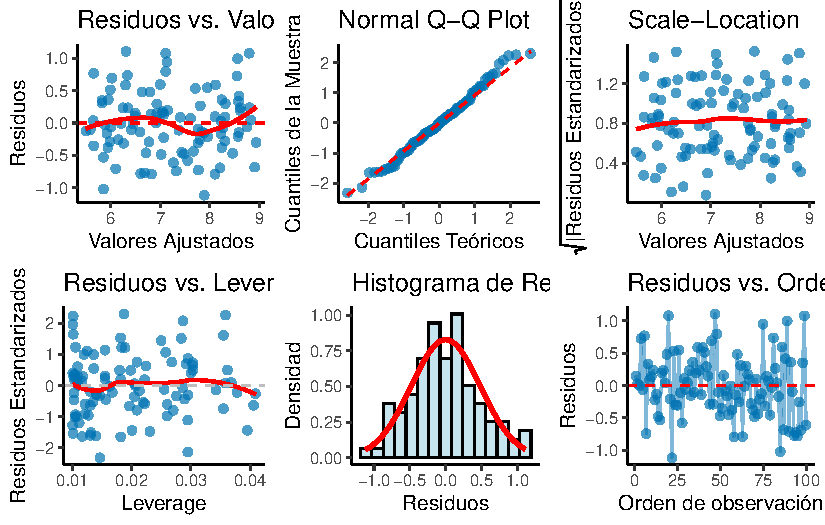
\includegraphics[keepaspectratio]{tema1_files/figure-pdf/fig-diagnostico-completo-1.pdf}}

}

\caption{\label{fig-diagnostico-completo}Gráficos de diagnóstico
completo del modelo de regresión.}

\end{figure}%

\textbf{Conclusión del diagnóstico:}

Nuestro modelo de estudio pasa exitosamente todas las verificaciones:

\textbf{✅ Linealidad}: Los gráficos de residuos vs valores ajustados no
muestran patrones sistemáticos, confirmando que la relación lineal es
apropiada.

\textbf{✅ Homocedasticidad}: La prueba de Breusch-Pagan arroja un
p-valor de 0.8886, que es mayor a 0.05, por lo que no hay evidencia de
heterocedasticidad. La varianza de los errores es constante.

\textbf{✅ Normalidad}: La prueba de Shapiro-Wilk presenta un p-valor de
0.671, superior a 0.05, confirmando que los residuos siguen una
distribución normal. Esto se corrobora visualmente en el Q-Q plot.

\textbf{✅ Independencia}: El estadístico de Durbin-Watson es 2.056 con
un p-valor de 0.61, indicando ausencia de autocorrelación en los
residuos.

\textbf{✅ Media nula}: La media de los residuos es 0, prácticamente
cero como se esperaría en un modelo bien especificado.

\begin{verbatim}
Se identificaron las siguientes observaciones que requieren atención:
• Alto apalancamiento (> 0.04 ): 24, 74
• Influyentes según Cook (> 0.041 ): 6, 20, 47, 85, 87, 89
• Influyentes según DFFITS (> 0.283 ): 6, 20, 22, 47, 85, 87, 89
• Posibles outliers (|residuo std| > 2): 20, 22, 47, 85, 89, 99

Estas observaciones deberían ser investigadas más detalladamente antes de proceder con las inferencias finales.
\end{verbatim}

Esto confirma que nuestras inferencias estadísticas (p-valores,
intervalos de confianza) son válidas y confiables (James et al. 2021;
Harrell 2015).

\end{tcolorbox}

\bookmarksetup{startatroot}

\chapter{El modelo de regresión lineal
múltiple}\label{sec-regresion-lineal-multiple}

El modelo de regresión lineal múltiple constituye la extensión natural y
más potente del modelo simple que estudiamos en el capítulo anterior.
Mientras que la regresión simple nos permitía examinar la relación entre
una variable respuesta y un único predictor, la regresión múltiple nos
capacita para \textbf{modelar simultáneamente el efecto de múltiples
variables predictoras}, una situación mucho más realista en la mayoría
de aplicaciones prácticas (Kutner et al. 2005; James et al. 2021; Fox
and Weisberg 2018).

En este capítulo profundizaremos en los aspectos únicos de la regresión
múltiple que no están presentes en el caso simple: la
\textbf{interpretación de coeficientes en presencia de otros
predictores}, el \textbf{diagnóstico específico} del modelo múltiple, y
el problema crucial de la \textbf{multicolinealidad}. Estos conceptos
son fundamentales para desarrollar modelos predictivos robustos y
interpretables (Harrell 2015; Draper 1998).

\begin{tcolorbox}[enhanced jigsaw, leftrule=.75mm, breakable, colbacktitle=quarto-callout-important-color!10!white, bottomrule=.15mm, colframe=quarto-callout-important-color-frame, toprule=.15mm, colback=white, coltitle=black, bottomtitle=1mm, left=2mm, title=\textcolor{quarto-callout-important-color}{\faExclamation}\hspace{0.5em}{Objetivos de aprendizaje}, opacityback=0, arc=.35mm, opacitybacktitle=0.6, toptitle=1mm, titlerule=0mm, rightrule=.15mm]

Al finalizar este capítulo, serás capaz de:

\begin{enumerate}
\def\labelenumi{\arabic{enumi}.}
\tightlist
\item
  \textbf{Formular y estimar} modelos de regresión lineal múltiple,
  comprendiendo las diferencias clave respecto al caso simple.
\item
  \textbf{Interpretar coeficientes} en el contexto multivariante,
  entendiendo el concepto de \emph{ceteris paribus} (``manteniendo las
  demás variables constantes'').
\item
  \textbf{Realizar inferencia estadística} construyendo intervalos de
  confianza y contrastes de hipótesis para los parámetros del modelo
  múltiple.
\item
  \textbf{Evaluar la calidad del ajuste} usando medidas como \(R^2\),
  \(R^2\) ajustado y la descomposición ANOVA.
\item
  \textbf{Diagnosticar el modelo múltiple}, aplicando técnicas
  específicas como gráficos CPR y gráficos de regresión parcial.
\item
  \textbf{Identificar y tratar la multicolinealidad}, comprendiendo sus
  causas, consecuencias y usando el VIF como herramienta de diagnóstico.
\item
  \textbf{Realizar predicciones} con el modelo ajustado, distinguiendo
  entre intervalos de confianza e intervalos de predicción.
\end{enumerate}

\end{tcolorbox}

\section{Formulación teórica del
modelo}\label{formulaciuxf3n-teuxf3rica-del-modelo-1}

El paso de la regresión simple a la múltiple es más que una simple
adición de términos; es un salto conceptual. Nos permite construir
modelos que reflejan mejor la complejidad del mundo real, donde los
resultados raramente dependen de una única causa. Al controlar
simultáneamente por varios factores, podemos aislar con mayor precisión
el efecto de una variable de interés, reduciendo el riesgo de llegar a
conclusiones sesgadas por variables omitidas.

\subsection{El modelo poblacional}\label{el-modelo-poblacional}

Para \(n\) observaciones y \(p\) variables predictoras, el
\textbf{modelo poblacional} postula que la relación verdadera entre la
variable respuesta \(Y\) y los predictores \(X_1, X_2, \ldots, X_p\)
sigue una relación lineal:

\[Y_i = \beta_0 + \beta_1 X_{i1} + \beta_2 X_{i2} + \cdots + \beta_p X_{ip} + \varepsilon_i, \quad i = 1,\dots,n\]

Donde \(Y_i\) es la \(i\)-ésima variable respuesta aleatoria, \(X_{ij}\)
es la \(i\)-ésima variable predictora aleatoria del \(j\)-ésimo
predictor, y \(\varepsilon_i\) es el término de error aleatorio. Los
parámetros \(\beta_0, \beta_1, \ldots, \beta_p\) son los coeficientes
poblacionales verdaderos pero desconocidos.

\subsection{El modelo muestral}\label{el-modelo-muestral}

En la práctica, trabajamos con datos observados y estimamos el modelo
usando la muestra disponible:

\[\hat{y}_i = \hat{\beta}_0 + \hat{\beta}_1 x_{i1} + \hat{\beta}_2 x_{i2} + \cdots + \hat{\beta}_p x_{ip}, \quad i = 1,\dots,n\]

Donde \(\hat{y}_i\) es la \(i\)-ésima predicción, \(x_{ij}\) es la
\(i\)-ésima observación del \(j\)-ésimo predictor, y \(\hat{\beta}_j\)
son los coeficientes estimados. El coeficiente \(\hat{\beta}_j\)
representa el cambio estimado en la media de \(Y\) ante un cambio de una
unidad en el predictor \(X_j\), \textbf{manteniendo constantes todas las
demás variables predictoras del modelo}. Este principio, conocido como
\emph{ceteris paribus} (del latín, ``lo demás constante''), es la piedra
angular de la interpretación en regresión múltiple.

\subsection{Notación matricial}\label{notaciuxf3n-matricial}

La notación matricial es fundamental para el desarrollo teórico y
computacional. Nos permite expresar el sistema de \(n\) ecuaciones de
forma compacta y elegante.

\textbf{Modelo poblacional:}
\[\mathbf{Y} = \tilde{X}\boldsymbol{\beta} + \boldsymbol{\varepsilon}\]

donde:

\[\mathbf{Y} = \begin{bmatrix} Y_1 \\ Y_2 \\ \vdots \\ Y_n \end{bmatrix}, \quad
\tilde{X} = \begin{bmatrix}
1 & X_{11} & X_{12} & \cdots & X_{1p} \\
1 & X_{21} & X_{22} & \cdots & X_{2p} \\
\vdots & \vdots & \vdots & \ddots & \vdots \\
1 & X_{n1} & X_{n2} & \cdots & X_{np}
\end{bmatrix}, \quad
\boldsymbol{\beta} = \begin{bmatrix} \beta_0 \\ \beta_1 \\ \vdots \\ \beta_p \end{bmatrix}, \quad
\boldsymbol{\varepsilon} = \begin{bmatrix} \varepsilon_1 \\ \varepsilon_2 \\ \vdots \\ \varepsilon_n \end{bmatrix}\]

Donde \(\tilde{X}\) contiene variables aleatorias (denotadas con
mayúsculas \(X_{ij}\)).

\textbf{Modelo muestral:}
\[\hat{\mathbf{y}} = \mathbf{X}\hat{\boldsymbol{\beta}}\]

donde:

\[\hat{\mathbf{y}} = \begin{bmatrix} \hat{y}_1 \\ \hat{y}_2 \\ \vdots \\ \hat{y}_n \end{bmatrix}, \quad
\mathbf{X} = \begin{bmatrix}
1 & x_{11} & x_{12} & \cdots & x_{1p} \\
1 & x_{21} & x_{22} & \cdots & x_{2p} \\
\vdots & \vdots & \vdots & \ddots & \vdots \\
1 & x_{n1} & x_{n2} & \cdots & x_{np}
\end{bmatrix}, \quad
\hat{\boldsymbol{\beta}} = \begin{bmatrix} \hat{\beta}_0 \\ \hat{\beta}_1 \\ \vdots \\ \hat{\beta}_p \end{bmatrix}\]

Donde \(\mathbf{X}\) contiene datos observados (denotados con minúsculas
\(x_{ij}\)).

La matriz \(\mathbf{X}\) (datos observados) y \(\tilde{X}\) (variables
aleatorias), ambas de dimensión \(n \times (p+1)\), se denominan
\textbf{matriz de diseño} y contienen toda la información de los
predictores. La primera columna de unos corresponde al término del
intercepto \(\beta_0\).

\subsection{Supuestos del modelo lineal
múltiple}\label{supuestos-del-modelo-lineal-muxfaltiple}

Para que nuestros estimadores tengan propiedades deseables (como ser
insesgados y eficientes), el modelo debe cumplir una serie de supuestos
sobre el comportamiento del término de error, conocidos como las
\textbf{condiciones de Gauss-Markov} (Kutner et al. 2005; Weisberg
2005).

\begin{enumerate}
\def\labelenumi{\arabic{enumi}.}
\item
  \textbf{Linealidad en los parámetros}: El valor esperado de la
  respuesta es una función lineal de los parámetros
  \(\boldsymbol{\beta}\). El modelo
  \(E[\mathbf{Y}|\tilde{X}] = \tilde{X}\boldsymbol{\beta}\) está bien
  especificado.
\item
  \textbf{Exogeneidad (media del error nula)}: Los errores tienen una
  media de cero para cualquier valor de los predictores,
  \(E[\boldsymbol{\varepsilon}|\tilde{X}] = \mathbf{0}\). Esto implica
  que los predictores no contienen información sobre el término de
  error.
\item
  \textbf{Homocedasticidad e independencia}: Los errores no están
  correlacionados entre sí y tienen una varianza constante \(\sigma^2\)
  para cualquier valor de los predictores. En notación matricial:
  \(\text{Var}(\boldsymbol{\varepsilon}|\tilde{X}) = \sigma^2\mathbf{I}_n\).
\item
  \textbf{Ausencia de multicolinealidad perfecta}: Ningún predictor es
  una combinación lineal exacta de los otros. Esto asegura que la matriz
  \(\mathbf{X}\) tiene rango completo \((p+1)\), lo cual es necesario
  para poder estimar de forma única todos los coeficientes.
\item
  \textbf{Normalidad de los errores (para inferencia)}: Para poder
  realizar contrastes de hipótesis e intervalos de confianza, se añade
  el supuesto de que los errores siguen una distribución Normal:
  \(\boldsymbol{\varepsilon} \sim N(\mathbf{0}, \sigma^2\mathbf{I}_n)\).
\end{enumerate}

\section{Estimación de los
parámetros}\label{estimaciuxf3n-de-los-paruxe1metros-1}

Una vez definido el modelo y sus supuestos, el siguiente paso es estimar
los parámetros desconocidos del vector \(\boldsymbol{\beta}\). El método
más extendido es el de Mínimos Cuadrados Ordinarios.

\subsection{El principio de mínimos cuadrados y la función
objetivo}\label{el-principio-de-muxednimos-cuadrados-y-la-funciuxf3n-objetivo}

La idea de ``mejor ajuste'' se traduce matemáticamente en minimizar la
discrepancia entre los valores observados \(\mathbf{y}\) (datos
muestrales) y los valores predichos por el modelo,
\(\hat{\mathbf{y}} = \mathbf{X}\hat{\boldsymbol{\beta}}\). Esta
discrepancia se captura a través de los residuos,
\(\mathbf{e} = \mathbf{y} - \hat{\mathbf{y}}\).

MCO no minimiza simplemente los residuos (ya que residuos positivos y
negativos se cancelarían), sino la \textbf{Suma de los Cuadrados de los
Residuos} (SCR o \emph{SSR} en inglés). Al elevarlos al cuadrado, nos
aseguramos de que todos los errores contribuyan positivamente y, además,
penalizamos más fuertemente los errores grandes.

La función objetivo a minimizar, \(S(\boldsymbol{\beta})\), usando datos
observados es:

\[S(\boldsymbol{\beta}) = \sum_{i=1}^n e_i^2 = \mathbf{e}^T\mathbf{e} = (\mathbf{y} - \mathbf{X}\boldsymbol{\beta})^T(\mathbf{y} - \mathbf{X}\boldsymbol{\beta})\]

\subsection{Derivación de las ecuaciones
normales}\label{derivaciuxf3n-de-las-ecuaciones-normales}

Para encontrar el vector \(\hat{\boldsymbol{\beta}}\) que minimiza esta
función, utilizamos cálculo diferencial. Primero, expandimos la
expresión cuadrática de \(S(\boldsymbol{\beta})\):

\[S(\boldsymbol{\beta}) = (\mathbf{y}^T - \boldsymbol{\beta}^T\mathbf{X}^T)(\mathbf{y} - \mathbf{X}\boldsymbol{\beta})\]
\[S(\boldsymbol{\beta}) = \mathbf{y}^T\mathbf{y} - \mathbf{y}^T\mathbf{X}\boldsymbol{\beta} - \boldsymbol{\beta}^T\mathbf{X}^T\mathbf{y} + \boldsymbol{\beta}^T\mathbf{X}^T\mathbf{X}\boldsymbol{\beta}\]

Un punto clave aquí es notar que
\(\boldsymbol{\beta}^T\mathbf{X}^T\mathbf{y}\) es un escalar (una matriz
\(1 \times 1\)), por lo que es igual a su transpuesta:
\(\boldsymbol{\beta}^T\mathbf{X}^T\mathbf{y} = \mathbf{y}^T\mathbf{X}\boldsymbol{\beta}\).
\(1 \times 1\)). Por lo tanto, es igual a su propia transpuesta:
\((\boldsymbol{\beta}^T\mathbf{X}^T\mathbf{y})^T = \mathbf{y}^T\mathbf{X}\boldsymbol{\beta}\).
Esto nos permite simplificar la expresión:

\[S(\boldsymbol{\beta}) = \mathbf{y}^T\mathbf{y} - 2\boldsymbol{\beta}^T\mathbf{X}^T\mathbf{y} + \boldsymbol{\beta}^T(\mathbf{X}^T\mathbf{X})\boldsymbol{\beta}\]

Ahora, derivamos esta función con respecto al vector
\(\boldsymbol{\beta}\) e igualamos el resultado a un vector de ceros
para encontrar el mínimo. Usando las reglas de la derivación matricial:

\begin{itemize}
\tightlist
\item
  La derivada de \(\mathbf{y}^T\mathbf{y}\) respecto a
  \(\boldsymbol{\beta}\) es \(\mathbf{0}\).
\item
  La derivada de \(2\boldsymbol{\beta}^T\mathbf{X}^T\mathbf{y}\)
  respecto a \(\boldsymbol{\beta}\) es \(2\mathbf{X}^T\mathbf{y}\).
\item
  La derivada de la forma cuadrática
  \(\boldsymbol{\beta}^T(\mathbf{X}^T\mathbf{X})\boldsymbol{\beta}\)
  respecto a \(\boldsymbol{\beta}\) es
  \(2(\mathbf{X}^T\mathbf{X})\boldsymbol{\beta}\).
\end{itemize}

Aplicando estas reglas, obtenemos el gradiente de la función de pérdida:

\[\frac{\partial S(\boldsymbol{\beta})}{\partial \boldsymbol{\beta}} = -2\mathbf{X}^T\mathbf{y} + 2(\mathbf{X}^T\mathbf{X})\boldsymbol{\beta}\]

Igualando a cero y sustituyendo \(\boldsymbol{\beta}\) por el estimador
\(\hat{\boldsymbol{\beta}}\) que cumple esta condición:

\[-2\mathbf{X}^T\mathbf{y} + 2(\mathbf{X}^T\mathbf{X})\hat{\boldsymbol{\beta}} = \mathbf{0}\]

Simplificando, llegamos al célebre sistema de \(p+1\) ecuaciones
conocido como las \textbf{Ecuaciones Normales}:

\[(\mathbf{X}^T\mathbf{X})\hat{\boldsymbol{\beta}} = \mathbf{X}^T\mathbf{y}\]

\subsection{La solución MCO y la condición de
invertibilidad}\label{la-soluciuxf3n-mco-y-la-condiciuxf3n-de-invertibilidad}

Para resolver este sistema y despejar \(\hat{\boldsymbol{\beta}}\),
necesitamos multiplicar por la inversa de la matriz
\((\mathbf{X}^T\mathbf{X})\). Esta inversa existe si y solo si la matriz
es invertible, lo que está directamente garantizado por el
\textbf{supuesto de ausencia de multicolinealidad perfecta}.

Si el rango de la matriz de diseño \(\mathbf{X}\) es \(p+1\) (sus
columnas son linealmente independientes), entonces la matriz
\(\mathbf{X}^T\mathbf{X}\) (de dimensión \((p+1) \times (p+1)\)) será de
rango completo, simétrica y definida positiva, y por tanto, invertible.

La solución única para el vector de estimadores MCO es:

\[\hat{\boldsymbol{\beta}} = (\mathbf{X}^T\mathbf{X})^{-1}\mathbf{X}^T\mathbf{y}\]

Esta compacta y poderosa ecuación es la base de la estimación en
regresión lineal y es implementada por todo el software estadístico.

Claro, aquí tienes el texto completo en formato Markdown y con las
fórmulas clave sin los recuadros.

\subsection{Propiedades de los estimadores de
MCO}\label{propiedades-de-los-estimadores-de-mco-1}

Una vez que hemos obtenido la fórmula para calcular nuestros
coeficientes,
\(\hat{\boldsymbol{\beta}} = (\mathbf{X}^T\mathbf{X})^{-1}\mathbf{X}^T\mathbf{y}\),
la pregunta fundamental es: ¿qué tan buenos son estos estimadores? La
teoría estadística nos proporciona una respuesta contundente a través de
sus propiedades en el muestreo, que son la base para toda la inferencia
estadística posterior.

El \textbf{Teorema de Gauss-Markov} es el resultado central. Afirma que,
si se cumplen los supuestos del modelo lineal clásico (1-4), los
estimadores de Mínimos Cuadrados Ordinarios son los \textbf{Mejores
Estimadores Lineales Insesgados (MELI o BLUE)}. Desglosemos esto:

\begin{itemize}
\tightlist
\item
  \textbf{Lineal}: \(\hat{\boldsymbol{\beta}}\) es una combinación
  lineal de la variable respuesta \(\mathbf{y}\).
\item
  \textbf{Insesgado (Unbiased)}: En promedio, a lo largo de infinitas
  muestras, nuestro estimador acertará al verdadero valor poblacional
  \(\boldsymbol{\beta}\). No tiene un sesgo sistemático. La demostración
  formal es directa: \begin{align}
    E[\hat{\boldsymbol{\beta}}] &= E[(\mathbf{X}^T\mathbf{X})^{-1}\mathbf{X}^T\mathbf{y}] \nonumber \\
    &= E[(\mathbf{X}^T\mathbf{X})^{-1}\mathbf{X}^T(\mathbf{X}\boldsymbol{\beta} + \boldsymbol{\varepsilon})] \nonumber \\
    &= (\mathbf{X}^T\mathbf{X})^{-1}\mathbf{X}^T\mathbf{X}\boldsymbol{\beta} + (\mathbf{X}^T\mathbf{X})^{-1}\mathbf{X}^T E[\boldsymbol{\varepsilon}] \nonumber \\
    &= \boldsymbol{I}\boldsymbol{\beta} + \mathbf{0} = \boldsymbol{\beta} \nonumber
    \end{align}
\item
  \textbf{Mejor (Best)}: ``Mejor'' significa que tiene la mínima
  varianza posible dentro de la clase de todos los estimadores lineales
  e insesgados. No existe otro estimador de este tipo que sea más
  preciso. La precisión de nuestros estimadores se captura en su
  \textbf{matriz de varianzas-covarianzas}: \begin{align}
    \text{Var}(\hat{\boldsymbol{\beta}}) &= \text{Var}[(\mathbf{X}^T\mathbf{X})^{-1}\mathbf{X}^T\mathbf{y}] \nonumber \\
    &= (\mathbf{X}^T\mathbf{X})^{-1}\mathbf{X}^T \, \text{Var}(\mathbf{y}) \, [(\mathbf{X}^T\mathbf{X})^{-1}\mathbf{X}^T]^T \nonumber \\
    &= (\mathbf{X}^T\mathbf{X})^{-1}\mathbf{X}^T \, (\sigma^2 \mathbf{I}_n) \, \mathbf{X}(\mathbf{X}^T\mathbf{X})^{-1} \nonumber \\
    &= \sigma^2 (\mathbf{X}^T\mathbf{X})^{-1}\mathbf{X}^T\mathbf{X}(\mathbf{X}^T\mathbf{X})^{-1} \nonumber \\
    &= \sigma^2 (\mathbf{X}^T\mathbf{X})^{-1} \nonumber
    \end{align} Por tanto, la matriz que define la incertidumbre de
  nuestro estimador es:
  \[\text{Var}(\hat{\boldsymbol{\beta}}) = \sigma^2(\mathbf{X}^T\mathbf{X})^{-1}\]
  Los elementos de la diagonal de esta matriz nos dan la varianza de
  cada coeficiente individual, \(Var(\hat{\beta}_j)\), mientras que los
  elementos fuera de la diagonal nos dan la covarianza entre pares de
  coeficientes, \(Cov(\hat{\beta}_j, \hat{\beta}_k)\).
\end{itemize}

Finalmente, si añadimos el \textbf{supuesto de normalidad de los
errores} (\(\varepsilon_i \sim N(0, \sigma^2)\)), las propiedades del
estimador se completan. Dado que \(\hat{\boldsymbol{\beta}}\) es una
combinación lineal de \(\mathbf{y}\) (que ahora es normal), el propio
estimador seguirá una distribución normal:
\[\hat{\boldsymbol{\beta}} \sim N\left(\boldsymbol{\beta}, \sigma^2(\mathbf{X}^T\mathbf{X})^{-1}\right)\]Esto
implica que cada coeficiente individual también se distribuye
normalmente:\[\hat{\beta}_j \sim N\left(\beta_j, \sigma^2 [(\mathbf{X}^T\mathbf{X})^{-1}]_{jj}\right)\]
donde \([(\mathbf{X}^T\mathbf{X})^{-1}]_{jj}\) es el j-ésimo elemento de
la diagonal de la matriz inversa. Este resultado es la puerta de entrada
a la inferencia, permitiéndonos construir intervalos de confianza y
realizar contrastes de hipótesis (como los test-t).

\subsection{Estimación de la varianza del
error}\label{estimaciuxf3n-de-la-varianza-del-error-1}

La matriz de varianzas-covarianzas de \(\hat{\boldsymbol{\beta}}\)
depende de \(\sigma^2\), la varianza de los errores poblacionales, que
es desconocida. Por lo tanto, el siguiente paso lógico es encontrar un
buen estimador para ella a partir de nuestros datos.

El punto de partida natural son los residuos del modelo,
\(\mathbf{e} = \mathbf{y} - \hat{\mathbf{y}}\), que son la contraparte
muestral de los errores teóricos \(\boldsymbol{\varepsilon}\). La suma
de los cuadrados de los residuos (SSE) es la base de nuestro estimador:

\[SSE = \mathbf{e}^T\mathbf{e} = \mathbf{y}^T(\mathbf{I}_n - \mathbf{H})^T(\mathbf{I}_n - \mathbf{H})\mathbf{y} = \mathbf{y}^T(\mathbf{I}_n - \mathbf{H})\mathbf{y}\]
(usando las propiedades de simetría e idempotencia de la matriz de
proyección \(\mathbf{H}\)).

Para encontrar un estimador insesgado, calculamos el valor esperado de
la SSE. Utilizando el lema
\(E[\mathbf{z}^T\mathbf{A}\mathbf{z}] = \text{traza}(\mathbf{A}\boldsymbol{\Sigma}) + \boldsymbol{\mu}^T\mathbf{A}\boldsymbol{\mu}\)
con \(\mathbf{z} = \mathbf{y}\),
\(\mathbf{A} = \mathbf{I}_n - \mathbf{H}\),
\(\boldsymbol{\mu} = \mathbf{X}\boldsymbol{\beta}\) y
\(\boldsymbol{\Sigma} = \sigma^2\mathbf{I}_n\): \begin{align}
E[SSE] &= \text{traza}[(\mathbf{I}_n - \mathbf{H})\sigma^2\mathbf{I}_n] + \boldsymbol{\beta}^T\mathbf{X}^T(\mathbf{I}_n - \mathbf{H})\mathbf{X}\boldsymbol{\beta} \nonumber
\end{align} El segundo término se anula porque
\((\mathbf{I}_n - \mathbf{H})\mathbf{X} = \mathbf{X} - \mathbf{H}\mathbf{X} = \mathbf{X} - \mathbf{X} = \mathbf{0}\).
Nos queda: \begin{align}
E[SSE] &= \sigma^2 \text{traza}(\mathbf{I}_n - \mathbf{H}) \nonumber \\
&= \sigma^2 (\text{traza}(\mathbf{I}_n) - \text{traza}(\mathbf{H})) \nonumber \\
&= \sigma^2 (n - (p + 1)) \nonumber
\end{align} El valor esperado de la SSE no es \(\sigma^2\), sino un
múltiplo de ella. Esto nos lleva directamente a un estimador insesgado
para \(\sigma^2\) dividiendo la SSE por sus \textbf{grados de libertad},
\(n - p - 1\):
\[\hat{\sigma}^2 = s^2 = \frac{SSE}{n - p - 1} = \frac{\mathbf{e}^T\mathbf{e}}{n - p - 1}\]
Intuitivamente, perdemos un grado de libertad por cada parámetro que
hemos estimado en el modelo (los \(p\) coeficientes de las pendientes y
el intercepto). La raíz cuadrada de este valor, \(\hat{\sigma}\), se
conoce como el \textbf{Error Estándar de la Regresión} y representa la
magnitud de un error de predicción típico.

Con este estimador, podemos calcular el \textbf{error estándar de cada
coeficiente}, que mide la incertidumbre de nuestra estimación para
\(\beta_j\):
\[\text{se}(\hat{\beta}_j) = \sqrt{\hat{\sigma}^2 [(\mathbf{X}^T\mathbf{X})^{-1}]_{jj}}\]
Bajo normalidad, se puede demostrar además que la cantidad
\(\frac{SSE}{\sigma^2}\) sigue una distribución \textbf{Chi-cuadrado}
con \(n-p-1\) grados de libertad, un resultado clave para la inferencia
formal.

\begin{tcolorbox}[enhanced jigsaw, leftrule=.75mm, breakable, colbacktitle=quarto-callout-tip-color!10!white, bottomrule=.15mm, colframe=quarto-callout-tip-color-frame, toprule=.15mm, colback=white, coltitle=black, bottomtitle=1mm, left=2mm, title=\textcolor{quarto-callout-tip-color}{\faLightbulb}\hspace{0.5em}{Ejemplo: Estimación de un modelo múltiple}, opacityback=0, arc=.35mm, opacitybacktitle=0.6, toptitle=1mm, titlerule=0mm, rightrule=.15mm]

Para ilustrar estos conceptos, usemos un ejemplo con datos de precios de
viviendas. Supongamos que queremos predecir el precio de una vivienda
basándonos en su superficie, número de habitaciones, antigüedad,
distancia al centro y si tiene garaje.

\begin{verbatim}

Call:
lm(formula = precio ~ superficie + habitaciones + antiguedad + 
    distancia_centro + garaje, data = viviendas)

Residuals:
   Min     1Q Median     3Q    Max 
-38847 -11074    867   9898  38486 

Coefficients:
                 Estimate Std. Error t value Pr(>|t|)    
(Intercept)      53750.97    6666.71   8.063 7.53e-14 ***
superficie        1171.78      47.28  24.783  < 2e-16 ***
habitaciones     15072.31    1303.42  11.564  < 2e-16 ***
antiguedad        -744.59      75.42  -9.872  < 2e-16 ***
distancia_centro -2028.27     164.88 -12.302  < 2e-16 ***
garajeSí         25829.43    2349.44  10.994  < 2e-16 ***
---
Signif. codes:  0 '***' 0.001 '**' 0.01 '*' 0.05 '.' 0.1 ' ' 1

Residual standard error: 15950 on 194 degrees of freedom
Multiple R-squared:  0.9094,    Adjusted R-squared:  0.9071 
F-statistic: 389.4 on 5 and 194 DF,  p-value: < 2.2e-16
\end{verbatim}

Este output nos muestra:

\begin{itemize}
\tightlist
\item
  \textbf{Coeficientes estimados} (\(\hat{\boldsymbol{\beta}}\)) y sus
  errores estándar
\item
  \textbf{Estadísticos t} y p-valores para cada coeficiente
\item
  \textbf{Error estándar residual} (\$\hat{\sigma} =
  \ensuremath{1.5952\times 10^{4}} euros)
\item
  \textbf{R² múltiple} (0.9094) - proporción de varianza explicada
\item
  \textbf{Estadístico F global} para contrastar la significancia del
  modelo
\end{itemize}

\end{tcolorbox}

\section{La interpretación de los
coeficientes}\label{la-interpretaciuxf3n-de-los-coeficientes}

Estimar los coeficientes y sus errores estándar es solo la mitad del
trabajo. La otra mitad, y a menudo la más importante, es interpretarlos
correctamente.

El concepto fundamental en regresión múltiple es el de \textbf{ceteris
paribus} (``lo demás constante''). Cada coeficiente \(\beta_j\)
representa el cambio esperado en \(Y\) por un cambio de una unidad en
\(X_j\), \textbf{manteniendo todas las demás variables predictoras del
modelo fijas}. Es el efecto ``puro'' o ``aislado'' de \(X_j\) sobre
\(Y\), después de haber controlado por la influencia de las otras
variables incluidas en el modelo. Matemáticamente, es la derivada
parcial del valor esperado de \(Y\) con respecto a \(X_j\):
\[\beta_j = \frac{\partial E[Y|\tilde{X}]}{\partial X_j}\]

Esta interpretación es crucialmente diferente de la que se obtiene en
una regresión simple. El coeficiente de una regresión simple de \(Y\)
sobre \(X_j\) captura no solo el efecto directo de \(X_j\), sino también
los efectos indirectos de cualquier otra variable omitida que esté
correlacionada tanto con \(Y\) como con \(X_j\). Por ello, el valor de
\(\hat{\beta}_j\) en una regresión múltiple casi nunca es igual al de
una regresión simple.

La forma más precisa de entender \(\hat{\beta}_j\) es a través del
concepto de \textbf{regresión parcial}. El coeficiente \(\hat{\beta}_j\)
de la regresión múltiple es idéntico al coeficiente de una regresión
simple entre dos conjuntos de residuos:

\begin{enumerate}
\def\labelenumi{\arabic{enumi}.}
\tightlist
\item
  Los residuos de una regresión de \(\mathbf{y}\) sobre todas las demás
  variables predictoras (excepto \(X_j\)).
\item
  Los residuos de una regresión de \(\mathbf{x_j}\) sobre todas las
  demás variables predictoras.
\end{enumerate}

En otras palabras, \(\hat{\beta}_j\) mide la relación entre la parte de
\(Y\) que no puede ser explicada por las otras variables y la parte de
\(X_j\) que tampoco puede ser explicada por las otras variables. Es la
asociación entre \(Y\) y \(X_j\) después de haber ``limpiado'' o
``netado'' la influencia de todos los demás predictores de ambas. Este
concepto se visualiza en los \textbf{gráficos de regresión parcial} (o
\emph{added-variable plots}), que son una herramienta de diagnóstico
fundamental.

\begin{tcolorbox}[enhanced jigsaw, leftrule=.75mm, breakable, colbacktitle=quarto-callout-tip-color!10!white, bottomrule=.15mm, colframe=quarto-callout-tip-color-frame, toprule=.15mm, colback=white, coltitle=black, bottomtitle=1mm, left=2mm, title=\textcolor{quarto-callout-tip-color}{\faLightbulb}\hspace{0.5em}{Interpretación práctica de los coeficientes}, opacityback=0, arc=.35mm, opacitybacktitle=0.6, toptitle=1mm, titlerule=0mm, rightrule=.15mm]

Volviendo a nuestro ejemplo de viviendas, interpretemos cada coeficiente
aplicando el principio \emph{ceteris paribus}:

\begin{itemize}
\item
  \textbf{Superficie} (1172 €/m²): Por cada metro cuadrado adicional, el
  precio aumenta en promedio 1172 euros, \textbf{manteniendo constantes}
  el número de habitaciones, antigüedad, distancia al centro y presencia
  de garaje.
\item
  \textbf{Habitaciones} (\ensuremath{1.5072\times 10^{4}} €): Cada
  habitación adicional incrementa el precio en
  \ensuremath{1.5072\times 10^{4}} euros en promedio,
  \textbf{controlando por} la superficie y demás variables.
\item
  \textbf{Antigüedad} (-745 €/año): Por cada año de antigüedad, el
  precio disminuye en 745 euros en promedio, \textbf{ceteris paribus}.
\item
  \textbf{Distancia al centro} (-2028 €/km): Cada kilómetro adicional de
  distancia reduce el precio en 2028 euros en promedio,
  \textbf{manteniendo todo lo demás constante}.
\item
  \textbf{Garaje} (\ensuremath{2.5829\times 10^{4}} €): Las viviendas
  con garaje cuestan \ensuremath{2.5829\times 10^{4}} euros más que las
  que no tienen, \textbf{en promedio y controlando por las demás
  variables}.
\end{itemize}

\textbf{Punto clave}: Estos efectos son diferentes de los que
obtendríamos con regresiones simples, ya que aquí hemos ``limpiado'' la
influencia de las otras variables.

\end{tcolorbox}

\begin{tcolorbox}[enhanced jigsaw, leftrule=.75mm, breakable, colbacktitle=quarto-callout-note-color!10!white, bottomrule=.15mm, colframe=quarto-callout-note-color-frame, toprule=.15mm, colback=white, coltitle=black, bottomtitle=1mm, left=2mm, title=\textcolor{quarto-callout-note-color}{\faInfo}\hspace{0.5em}{La perspectiva geométrica de mínimos cuadrados}, opacityback=0, arc=.35mm, opacitybacktitle=0.6, toptitle=1mm, titlerule=0mm, rightrule=.15mm]

La estimación por mínimos cuadrados tiene una interpretación geométrica
elegante y potente que nos ayuda a comprender qué está ocurriendo.

Podemos pensar en el vector de observaciones \(\mathbf{y}\) como un
punto en un espacio de \(n\) dimensiones. Las columnas de la matriz de
diseño \(\mathbf{X}\) generan un subespacio vectorial dentro de
\(\mathbb{R}^n\), conocido como el \textbf{espacio columna} de
\(\mathbf{X}\), denotado \(C(\mathbf{X})\). Este subespacio contiene
todas las posibles combinaciones lineales de nuestros predictores.

El método MCO encuentra el vector de valores ajustados
\(\hat{\mathbf{y}} = \mathbf{X}\hat{\boldsymbol{\beta}}\) que está ``más
cerca'' de \(\mathbf{y}\). Geométricamente, este punto no es otro que la
\textbf{proyección ortogonal} del vector \(\mathbf{y}\) sobre el
subespacio \(C(\mathbf{X})\).

Esta proyección se realiza a través de una matriz especial llamada
\textbf{matriz de proyección} o \textbf{matriz sombrero} (\emph{hat
matrix}), denotada por \(\mathbf{H}\):

\[\hat{\mathbf{y}} = \text{Proj}_{C(\mathbf{X})}\,\mathbf{y} = \mathbf{H}\,\mathbf{y}, \qquad \text{donde} \quad \mathbf{H} = \mathbf{X}(\mathbf{X}^T\mathbf{X})^{-1}\mathbf{X}^T\]

Esta operación induce la \textbf{descomposición ortogonal fundamental}
del vector de respuesta:

\[\mathbf{y} = \hat{\mathbf{y}} + \mathbf{e}\]

El hecho de que la proyección sea ortogonal implica que el vector de
residuos \(\mathbf{e}\) es ortogonal (perpendicular) al vector de
valores ajustados \(\hat{\mathbf{y}}\) y, de hecho, a todo el subespacio
\(C(\mathbf{X})\). Esta ortogonalidad,
\(\hat{\mathbf{y}}^T\mathbf{e}=0\), es la base del \textbf{Teorema de
Pitágoras para la regresión}, que permite la descomposición de la
variabilidad total en una parte explicada y una no explicada.

\end{tcolorbox}

\section{Evaluación del modelo y descomposición de la
varianza}\label{evaluaciuxf3n-del-modelo-y-descomposiciuxf3n-de-la-varianza}

Una vez estimado el modelo, el siguiente paso es evaluar su desempeño.
¿Qué tan bien se ajustan nuestras predicciones a los datos reales?
Aunque ya vimos la perspectiva geométrica y el Teorema de Pitágoras en
regresión simple, es importante revisitar estos conceptos porque en
regresión múltiple la interpretación y el cálculo de la descomposición
de varianza presenta matices adicionales que debemos entender
claramente.

En regresión múltiple, la \textbf{Descomposición de la Varianza} o
\textbf{ANOVA} (\emph{Analysis of Variance}) cobra especial relevancia
porque ahora tenemos múltiples variables explicativas y necesitamos
evaluar el aporte conjunto de todas ellas, así como su significancia
global.

La idea fundamental es que la variabilidad total de la variable
respuesta (\(Y\)) puede descomponerse en dos partes: una parte que es
explicada por nuestro modelo de regresión (ahora con múltiples
variables) y otra parte que queda sin explicar, atribuida al error
aleatorio.

Partimos de la identidad:
\((y_i - \bar{y}) = (\hat{y}_i - \bar{y}) + (y_i - \hat{y}_i) = (\hat{y}_i - \bar{y}) + e_i\).

Elevando al cuadrado y sumando para todas las observaciones (y gracias a
la propiedad de ortogonalidad \(\hat{\mathbf{y}}^T\mathbf{e}=0\), que
hace que los productos cruzados se anulen), llegamos a la descomposición
fundamental de las sumas de cuadrados:

\[\sum_{i=1}^n (y_i - \bar{y})^2 = \sum_{i=1}^n (\hat{y}_i - \bar{y})^2 + \sum_{i=1}^n e_i^2\]

Esto se conoce como la \textbf{ecuación de ANOVA}:

\[SST = SSR + SSE\]

Donde:

\begin{itemize}
\tightlist
\item
  \textbf{SST (Suma de Cuadrados Total)}: Es la variabilidad total de
  \(Y\). Mide la dispersión de los datos observados alrededor de su
  media.
\item
  \textbf{SSR (Suma de Cuadrados de la Regresión)}: Es la variabilidad
  \textbf{explicada} por el modelo. Mide la dispersión de los valores
  predichos alrededor de la media.
\item
  \textbf{SSE (Suma de Cuadrados del Error)}: Es la variabilidad
  \textbf{no explicada} o residual. Mide la dispersión de los datos
  observados alrededor de la línea de regresión.
\end{itemize}

Esta tabla no es solo un resumen; es el motor de las principales
herramientas de evaluación e inferencia del modelo.

\subsection{Coeficiente de determinación
múltiple}\label{coeficiente-de-determinaciuxf3n-muxfaltiple}

El \textbf{coeficiente de determinación}, \(R^2\), es la medida de
ajuste más popular. Responde a la pregunta: \emph{¿Qué proporción de la
variabilidad total de Y es explicada por las variables predictoras del
modelo?}

\[R^2 = \frac{SSR}{SST} = 1 - \frac{SSE}{SST}\]

\textbf{Propiedades clave}:

\begin{itemize}
\tightlist
\item
  Su valor siempre está entre 0 (el modelo no explica nada) y 1 (el
  modelo explica toda la variabilidad).
\item
  Puede interpretarse como el cuadrado de la correlación entre los
  valores observados y los valores predichos,
  \(R^2 = \text{corr}^2(\mathbf{y}, \hat{\mathbf{y}})\).
\item
  \textbf{Problema}: \(R^2\) \textbf{nunca decrece} al añadir una nueva
  variable predictora al modelo, incluso si esta es completamente
  irrelevante. Esto lo convierte en una métrica engañosa para comparar
  modelos con distinto número de predictores.
\end{itemize}

\subsection{El coeficiente de determinación
ajustado}\label{el-coeficiente-de-determinaciuxf3n-ajustado}

Para solucionar el problema de \(R^2\), utilizamos el \(R^2\) ajustado,
que introduce una penalización por cada variable añadida. Lo hace
comparando las varianzas (sumas de cuadrados divididas por sus grados de
libertad) en lugar de solo las sumas de cuadrados:

\[R^2_{adj} = 1 - \frac{SSE/(n-p-1)}{SST/(n-1)} = 1 - \frac{\hat{\sigma}^2}{s_Y^2}\]

Donde \(s_Y^2\) es la varianza muestral de \(Y\). El \(R^2_{ajustado}\)
solo aumentará si la nueva variable mejora el modelo más de lo que se
esperaría por puro azar. Es, por tanto, la métrica preferida para
comparar la calidad de ajuste de modelos anidados.

¡Excelente observación! Tienes toda la razón. En la sección de
``Inferencia'' me centré en los contrastes de hipótesis (el test t y el
test F) pero omití una parte igualmente importante que sí estaba en tu
Tema 1: la \textbf{construcción de intervalos de confianza para los
parámetros}.

Un contraste de hipótesis te da una respuesta de ``sí/no'' sobre la
significancia, pero un intervalo de confianza te ofrece un rango de
valores plausibles para el efecto, lo cual es mucho más informativo.

Aquí tienes una versión revisada y ampliada de la sección
\textbf{``Inferencia estadística en el modelo múltiple''} que incluye
explícitamente los intervalos de confianza, manteniendo el flujo que
hemos construido. Puedes reemplazar la sección anterior por esta.

\section{Inferencia Estadística en el Modelo
Múltiple}\label{inferencia-estaduxedstica-en-el-modelo-muxfaltiple}

La estimación nos da los valores de los coeficientes para nuestra
muestra, pero la inferencia nos permite usar esos valores para sacar
conclusiones sobre los parámetros de la población. ¿Son estos
coeficientes ``reales'' o podrían ser fruto del azar muestral? Para
responder, nos basamos en las propiedades distributivas de nuestros
estimadores.

\subsection{Contraste de hipótesis sobre los
coeficientes}\label{contraste-de-hipuxf3tesis-sobre-los-coeficientes}

El \textbf{test t} nos permite decidir si una variable predictora
\(X_j\) tiene una relación estadísticamente significativa con \(Y\),
después de controlar por el efecto de todas las demás variables en el
modelo.

\begin{itemize}
\tightlist
\item
  \textbf{Hipótesis}: La hipótesis nula es que el coeficiente es cero en
  la población (\(H_0: \beta_j = 0\)), lo que implicaría que \(X_j\) no
  tiene un efecto lineal sobre \(Y\) una vez que se consideran los otros
  predictores. La alternativa es que el coeficiente es distinto de cero
  (\(H_1: \beta_j \neq 0\)).
\item
  \textbf{Estadístico de contraste}: Construimos el estadístico t, que
  mide cuántos errores estándar separan nuestro coeficiente estimado del
  valor nulo (cero).
  \[\frac{\hat{\beta}_j - \beta_j}{\text{se}(\hat{\beta}_j)} \sim t_{n-p-1}\]
  Bajo la hipótesis nula, el estadístico que calculamos con nuestra
  muestra es \(t_{obs} = \hat{\beta}_j / \text{se}(\hat{\beta}_j)\).
\item
  \textbf{Decisión}: Comparamos el valor observado \(t_{obs}\) con la
  distribución t de Student con \(n-p-1\) grados de libertad. Si el
  \textbf{p-valor} asociado es suficientemente pequeño (normalmente
  \textless{} 0.05), rechazamos la hipótesis nula y concluimos que la
  variable es un predictor estadísticamente significativo.
\end{itemize}

\subsection{Intervalo de confianza para los
coeficientes}\label{intervalo-de-confianza-para-los-coeficientes}

Mientras que el test t nos da una decisión binaria, el \textbf{intervalo
de confianza} nos proporciona un \textbf{rango de valores plausibles}
para el verdadero parámetro poblacional \(\beta_j\). Es una herramienta
de estimación más informativa.

La estructura del intervalo se basa en la distribución t que acabamos de
ver:

\[\text{Estimación puntual} \pm (\text{Valor crítico}) \times (\text{Error estándar})\]

Para un nivel de confianza del \(100(1-\alpha)\%\), el intervalo para
\(\beta_j\) es:

\[\hat{\beta}_j \pm t_{\alpha/2, n-p-1} \cdot \text{se}(\hat{\beta}_j)\]

\begin{itemize}
\tightlist
\item
  \textbf{Interpretación}: Tenemos una confianza del \(100(1-\alpha)\%\)
  de que el verdadero valor del parámetro poblacional \(\beta_j\) se
  encuentra dentro de este rango.
\item
  \textbf{Dualidad con el Contraste de Hipótesis}: Existe una relación
  directa entre el intervalo de confianza y el test t. Si el valor 0
  \textbf{no está incluido} en el intervalo de confianza del 95\% para
  \(\hat{\beta}_j\), es matemáticamente equivalente a rechazar la
  hipótesis nula \(H_0: \beta_j = 0\) con un nivel de significancia
  \(\alpha=0.05\). Esto nos da dos formas de llegar a la misma
  conclusión sobre la significancia de un predictor.
\end{itemize}

\subsection{Inferencia sobre la significancia global del
modelo}\label{inferencia-sobre-la-significancia-global-del-modelo}

El \textbf{test F} evalúa si el modelo en su conjunto tiene poder
predictivo. Es decir, contrasta si \textbf{al menos uno} de los
predictores tiene una relación significativa con \(Y\).

\begin{itemize}
\tightlist
\item
  \textbf{Hipótesis}: La hipótesis nula es que todos los coeficientes de
  las pendientes son simultáneamente cero
  (\(H_0: \beta_1 = \beta_2 = \dots = \beta_p = 0\)), frente a la
  alternativa de que al menos uno es distinto de cero
  (\(H_1: \text{Algún } \beta_j \neq 0\)).
\item
  \textbf{Estadístico de contraste}: El estadístico F se construye a
  partir de la tabla ANOVA, comparando la varianza explicada por el
  modelo con la varianza residual, ajustando por sus respectivos grados
  de libertad.
  \[F = \frac{\text{Varianza Explicada}}{\text{Varianza No Explicada}} = \frac{SSR / p}{SSE / (n-p-1)}\]
\item
  \textbf{Decisión}: Comparamos el valor del estadístico F con una
  distribución F de Snedecor con \(p\) y \(n-p-1\) grados de libertad.
  Un p-valor pequeño indica que el modelo es globalmente significativo y
  que, como conjunto, nuestros predictores explican una parte de la
  variabilidad de \(Y\) que no es atribuible al azar.
\end{itemize}

El test F es una herramienta fundamental, ya que representa el primer
paso en la validación de cualquier modelo de regresión múltiple.

\begin{tcolorbox}[enhanced jigsaw, leftrule=.75mm, breakable, colbacktitle=quarto-callout-tip-color!10!white, bottomrule=.15mm, colframe=quarto-callout-tip-color-frame, toprule=.15mm, colback=white, coltitle=black, bottomtitle=1mm, left=2mm, title=\textcolor{quarto-callout-tip-color}{\faLightbulb}\hspace{0.5em}{Interpretación de las pruebas estadísticas}, opacityback=0, arc=.35mm, opacitybacktitle=0.6, toptitle=1mm, titlerule=0mm, rightrule=.15mm]

En nuestro ejemplo de viviendas:

\textbf{Prueba F global}:

\begin{itemize}
\tightlist
\item
  F(5, 194) = 389.45, p \textless{} 0.001
\item
  \textbf{Conclusión}: El modelo es globalmente significativo. Al menos
  una variable predictora tiene una relación real con el precio.
\end{itemize}

\textbf{Pruebas t individuales} (ejemplos):

\begin{itemize}
\tightlist
\item
  \textbf{Superficie}: t = 24.78, p \textless{} 0.001 →
  \textbf{Significativa}
\item
  \textbf{Garaje}: t = 10.99, p \textless{} 0.001 →
  \textbf{Significativa}
\end{itemize}

\textbf{Intervalos de confianza} (95\%):

\begin{itemize}
\tightlist
\item
  \textbf{Superficie}: {[}1079, 1265{]} euros/m²
\item
  No incluye el 0, confirma la significancia estadística
\end{itemize}

\textbf{Interpretación práctica}: Estamos 95\% confiados de que el
verdadero efecto de la superficie está entre 1079 y 1265 euros por m²,
controlando por las demás variables.

\end{tcolorbox}

\section{Predicción con el modelo
múltiple}\label{predicciuxf3n-con-el-modelo-muxfaltiple}

Una vez que hemos ajustado y validado nuestro modelo, podemos utilizarlo
para uno de sus propósitos más poderosos: hacer predicciones para nuevas
observaciones. Es fundamental distinguir entre dos objetivos de
predicción diferentes, ya que cada uno conlleva un nivel de
incertidumbre distinto.

Supongamos que tenemos un nuevo conjunto de valores para las variables
predictoras, representado por el vector
\(\mathbf{x}_0^T = [1, x_{01}, x_{02}, \dots, x_{0p}]\). La
\textbf{predicción puntual} en ambos casos es la misma:

\[\hat{y}_0 = \mathbf{x}_0^T \hat{\boldsymbol{\beta}}\]

Sin embargo, esta estimación puntual está sujeta a error. Para
cuantificar esta incertidumbre, construimos dos tipos de intervalos.

\subsection{Intervalo de confianza para la respuesta
media}\label{intervalo-de-confianza-para-la-respuesta-media-1}

Este intervalo responde a la pregunta: \emph{¿cuál es el valor
\textbf{promedio} de Y para todas las observaciones con las
características} \(\mathbf{x}_0\)? Su objetivo es acotar la posición de
la verdadera (pero desconocida) superficie de regresión poblacional en
el punto \(\mathbf{x}_0\).

La incertidumbre aquí proviene únicamente de la estimación de los
coeficientes \(\hat{\boldsymbol{\beta}}\). La varianza de esta
predicción media es:

\[\text{Var}(\hat{y}_0) = \text{Var}(\mathbf{x}_0^T \hat{\boldsymbol{\beta}}) = \mathbf{x}_0^T \text{Var}(\hat{\boldsymbol{\beta}}) \mathbf{x}_0 = \sigma^2 \mathbf{x}_0^T (\mathbf{X}^T\mathbf{X})^{-1} \mathbf{x}_0\]

Reemplazando \(\sigma^2\) por su estimador insesgado \(\hat{\sigma}^2\),
el \textbf{intervalo de confianza al} \(100(1-\alpha)\%\) para la
respuesta media \(E[Y|\mathbf{X}=\mathbf{x}_0]\) es:

\[\hat{y}_0 \pm t_{\alpha/2, n-p-1} \cdot \sqrt{\hat{\sigma}^2 \mathbf{x}_0^T (\mathbf{X}^T\mathbf{X})^{-1} \mathbf{x}_0}\]

\subsection{Intervalo de predicción para una observación
individual}\label{intervalo-de-predicciuxf3n-para-una-observaciuxf3n-individual}

Este intervalo responde a una pregunta más ambiciosa: \emph{¿entre qué
valores se encontrará la respuesta de una \textbf{única y nueva}
observación con las características} \(\mathbf{x}_0\)?

Este intervalo debe considerar \textbf{dos fuentes de incertidumbre}:

\begin{enumerate}
\def\labelenumi{\arabic{enumi}.}
\tightlist
\item
  La incertidumbre sobre la localización de la verdadera superficie de
  regresión (la misma que en el intervalo de confianza).
\item
  La variabilidad aleatoria inherente a una sola observación, que se
  desvía de la media poblacional (el error \(\varepsilon_0\), cuya
  varianza es \(\sigma^2\)).
\end{enumerate}

Por esta razón, un intervalo de predicción \textbf{siempre será más
ancho} que un intervalo de confianza para el mismo nivel de
significancia. La varianza del error de predicción es la suma de las dos
fuentes de varianza:

\[\text{Var}(y_0 - \hat{y}_0) = \text{Var}(\varepsilon_0) + \text{Var}(\hat{y}_0) = \sigma^2 + \sigma^2 \mathbf{x}_0^T (\mathbf{X}^T\mathbf{X})^{-1} \mathbf{x}_0\]

El \textbf{intervalo de predicción al} \(100(1-\alpha)\%\) para una
observación individual \(y_0\) es:

\[\hat{y}_0 \pm t_{\alpha/2, n-p-1} \cdot \sqrt{\hat{\sigma}^2 \left(1 + \mathbf{x}_0^T (\mathbf{X}^T\mathbf{X})^{-1} \mathbf{x}_0\right)}\]

La diferencia clave es el \textbf{``+1''} dentro de la raíz cuadrada,
que representa la varianza de la nueva observación. Visualmente, tanto
la banda de confianza como la de predicción son más estrechas cerca del
``centroide'' de los datos (la media multivariante de los predictores) y
se ensanchan a medida que nos alejamos hacia valores más extremos de los
predictores.

\section{Diagnóstico del modelo
múltiple}\label{diagnuxf3stico-del-modelo-muxfaltiple}

Al igual que en la regresión simple, una vez ajustado el modelo es
fundamental realizar un diagnóstico exhaustivo para verificar que los
supuestos del modelo lineal se cumplen. La fiabilidad de todas nuestras
inferencias (p-valores e intervalos de confianza) descansa sobre la
validez de estos supuestos. El proceso sigue basándose en el
\textbf{análisis de los residuos}, nuestra ventana a los errores
teóricos no observables (Fox and Weisberg 2018; Harrell 2015).

\subsection{Verificación de los supuestos
clásicos}\label{verificaciuxf3n-de-los-supuestos-cluxe1sicos}

Los supuestos de linealidad, homocedasticidad, normalidad e
independencia se verifican con herramientas muy similares a las vistas
en el capítulo anterior, por lo que aquí las resumiremos y presentaremos
una herramienta adicional para la linealidad.

\begin{itemize}
\tightlist
\item
  \textbf{Normalidad}: El \textbf{gráfico Q-Q} de los residuos
  estudentizados y el \textbf{test de Shapiro-Wilk} siguen siendo las
  herramientas principales para comprobar que los errores se distribuyen
  de forma Normal.
\item
  \textbf{Independencia}: Para datos de series temporales, el
  \textbf{gráfico de residuos contra el tiempo} y el \textbf{test de
  Durbin-Watson} se utilizan de la misma manera para detectar
  autocorrelación.
\item
  \textbf{Homocedasticidad (Varianza Constante)}: El \textbf{gráfico
  Scale-Location} y el \textbf{test de Breusch-Pagan} siguen siendo los
  métodos de referencia para detectar heterocedasticidad (patrones de
  embudo en la dispersión de los residuos).
\end{itemize}

Para la \textbf{linealidad}, el gráfico de \textbf{Residuos vs.~Valores
Ajustados} sigue siendo la primera herramienta a inspeccionar. Una nube
de puntos sin patrones alrededor del cero sugiere que la forma funcional
del modelo es globalmente correcta. Sin embargo, en el contexto
múltiple, este gráfico podría ocultar una relación no lineal con
\emph{una variable específica}. Para ello, disponemos de una herramienta
más precisa.

\subsubsection{Gráficos de componente más
residuo}\label{gruxe1ficos-de-componente-muxe1s-residuo}

El gráfico de Componente más Residuo (CPR o Partial Residual Plots) nos
permite visualizar la relación entre la variable respuesta y \textbf{un
único predictor} \(X_j\), ajustando por el efecto de todos los demás
predictores. Para cada predictor \(X_j\), el gráfico muestra:

\[\text{Residuo Parcial} = e_i + \hat{\beta}_j x_{ij} \quad \text{vs.} \quad x_{ij}\]

La pendiente de una línea ajustada a estos puntos es exactamente
\(\hat{\beta}_j\). Si la relación es lineal, los puntos deben seguir la
línea de regresión. Una desviación sistemática (una curva) sugiere que
la relación con esa variable específica no es lineal y que podría
necesitar una transformación (p.ej., logarítmica o cuadrática).

\begin{tcolorbox}[enhanced jigsaw, leftrule=.75mm, breakable, colbacktitle=quarto-callout-tip-color!10!white, bottomrule=.15mm, colframe=quarto-callout-tip-color-frame, toprule=.15mm, colback=white, coltitle=black, bottomtitle=1mm, left=2mm, title=\textcolor{quarto-callout-tip-color}{\faLightbulb}\hspace{0.5em}{Ejemplo práctico: Gráficos de componente + residuo}, opacityback=0, arc=.35mm, opacitybacktitle=0.6, toptitle=1mm, titlerule=0mm, rightrule=.15mm]

Los gráficos CPR nos permiten visualizar si la relación de cada
predictor con la respuesta es verdaderamente lineal:

\begin{Shaded}
\begin{Highlighting}[]
\CommentTok{\# Cargar librerías necesarias}
\FunctionTok{suppressPackageStartupMessages}\NormalTok{(}\FunctionTok{library}\NormalTok{(car))}

\CommentTok{\# Gráficos de Componente más Residuo (CPR)}
\FunctionTok{crPlots}\NormalTok{(modelo, }\AttributeTok{main =} \StringTok{"Gráficos de Componente + Residuo"}\NormalTok{)}
\end{Highlighting}
\end{Shaded}

\pandocbounded{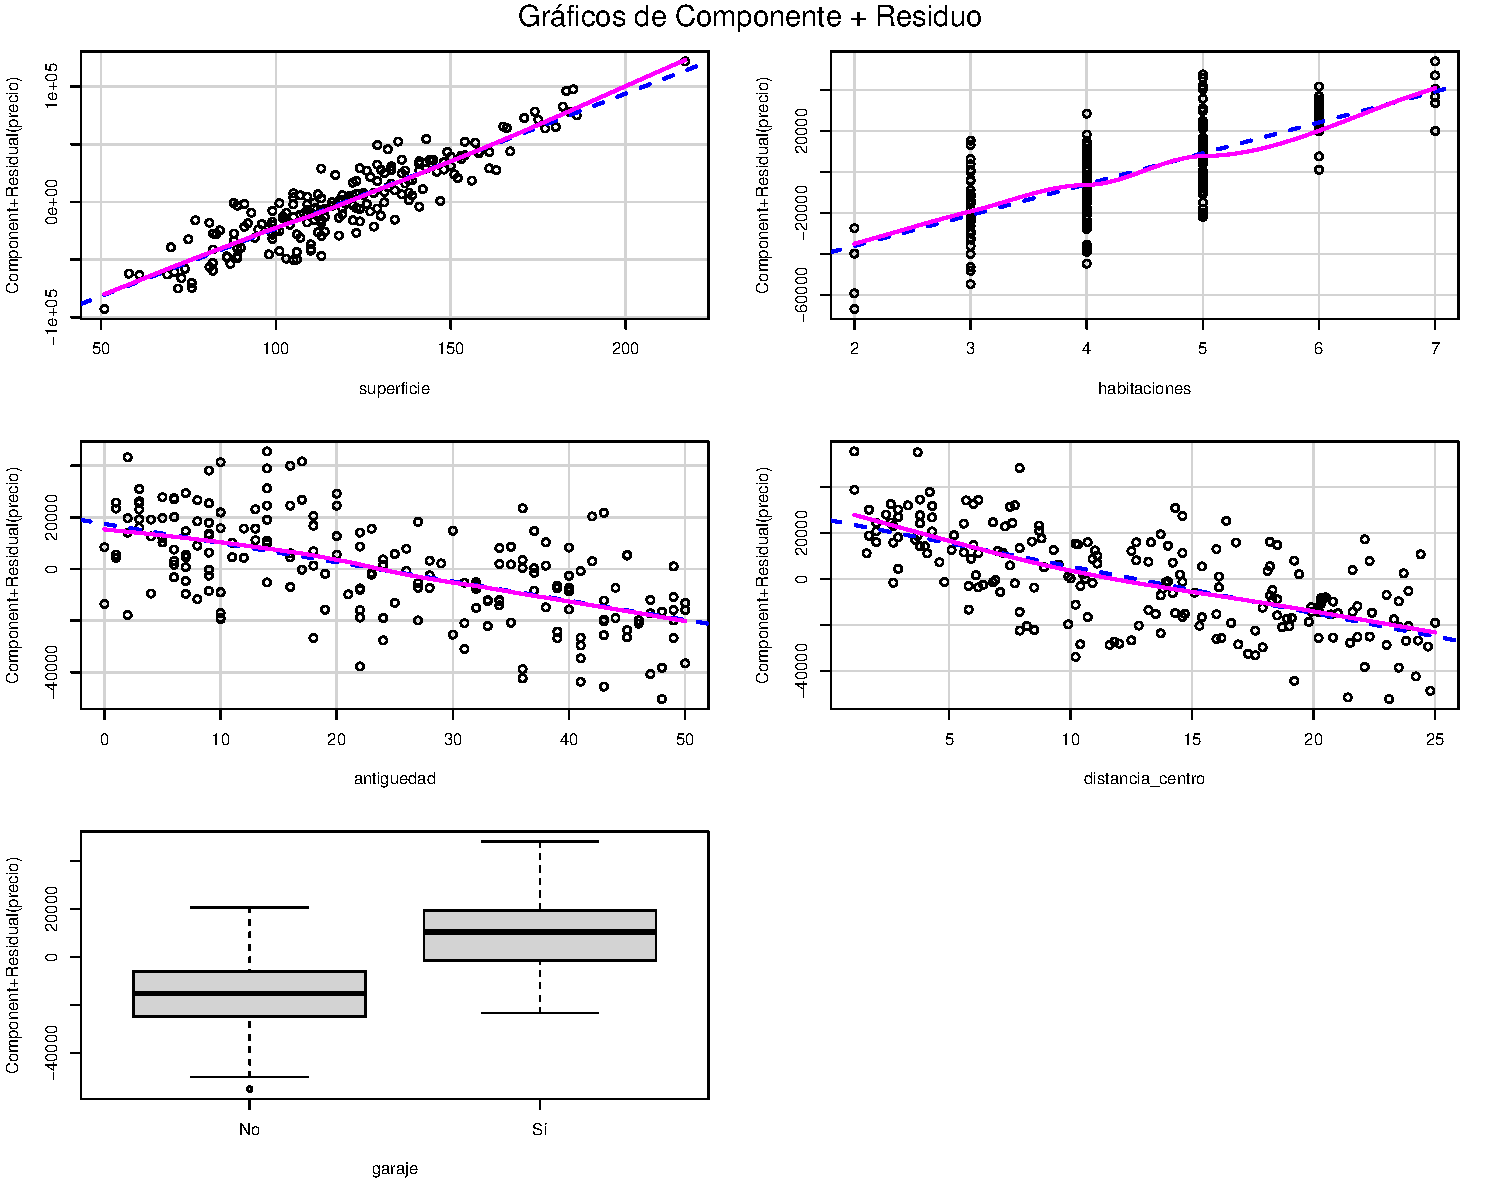
\includegraphics[keepaspectratio]{tema2_files/figure-pdf/diagnostico-cpr-1.pdf}}

\textbf{Interpretación:}

\begin{itemize}
\tightlist
\item
  \textbf{Línea sólida}: Muestra la relación lineal esperada (pendiente
  = coeficiente de regresión)
\item
  \textbf{Línea punteada}: Suavizado no paramétrico de los puntos
\item
  \textbf{Coincidencia de líneas}: Sugiere linealidad adecuada
\item
  \textbf{Divergencia significativa}: Indica posible no-linealidad que
  requiere transformación
\end{itemize}

Si vemos curvas sistemáticas en algún gráfico CPR, es señal de que esa
variable podría necesitar una transformación (log, cuadrática, etc.).

\end{tcolorbox}

\subsection{Diagnóstico de
multicolinealidad}\label{diagnuxf3stico-de-multicolinealidad}

La \textbf{multicolinealidad} es un problema que solo existe en la
regresión múltiple. Ocurre cuando dos o más variables predictoras están
fuertemente correlacionadas entre sí.

\subsubsection{Consecuencias de la
multicolinealidad}\label{consecuencias-de-la-multicolinealidad}

La multicolinealidad no viola los supuestos de Gauss-Markov (los
estimadores siguen siendo insesgados y eficientes), pero puede arruinar
la interpretación práctica de un modelo:

\begin{enumerate}
\def\labelenumi{\arabic{enumi}.}
\tightlist
\item
  \textbf{Varianza de los estimadores inflada}: Los errores estándar de
  los coeficientes de las variables colineales se vuelven muy grandes.
  Esto dificulta o imposibilita declarar un predictor como
  estadísticamente significativo, incluso si lo es.
\item
  \textbf{Inestabilidad de los coeficientes}: Pequeños cambios en los
  datos (o añadir/quitar una variable) pueden provocar cambios drásticos
  en las estimaciones de los coeficientes, incluso cambiando su signo,
  lo que hace que la interpretación sea poco fiable.
\item
  \textbf{Contradicciones en los contrastes}: Se puede dar la paradoja
  de tener un modelo globalmente significativo (test F con p-valor bajo
  y \(R^2\) alto) pero con ningún predictor individual significativo
  (tests t con p-valores altos).
\end{enumerate}

\subsubsection{Detección de la
multicolinealidad}\label{detecciuxf3n-de-la-multicolinealidad}

\begin{enumerate}
\def\labelenumi{\arabic{enumi}.}
\item
  \textbf{Matriz de correlaciones}: Un primer paso es examinar la matriz
  de correlaciones entre los predictores. Coeficientes de correlación
  altos (p.~ej., \textgreater{} 0.8) son una señal de alerta. Sin
  embargo, este método no detecta la colinealidad que involucra a tres o
  más variables.
\item
  \textbf{Factor de Inflación de la Varianza (VIF)}: Es la herramienta
  de diagnóstico definitiva. Para cada predictor \(X_j\), se calcula su
  VIF de la siguiente manera:

  \begin{enumerate}
  \def\labelenumii{\arabic{enumii}.}
  \tightlist
  \item
    Se ajusta una regresión lineal de \(X_j\) en función de
    \textbf{todas las demás variables predictoras}:
    \(X_j \sim X_1 + \dots + X_{j-1} + X_{j+1} + \dots + X_p\).
  \item
    Se obtiene el \(R^2\) de este modelo auxiliar, que llamamos
    \(R_j^2\). Este valor nos dice qué proporción de la varianza de
    \(X_j\) es explicada por los otros predictores.
  \item
    El VIF se calcula como: \[VIF_j = \frac{1}{1 - R_j^2}\]
  \end{enumerate}

  \begin{itemize}
  \tightlist
  \item
    \textbf{Interpretación}: El VIF nos dice por qué factor se infla la
    varianza del estimador \(\hat{\beta}_j\) debido a su relación con
    los otros predictores.
  \end{itemize}
\end{enumerate}

\begin{tcolorbox}[enhanced jigsaw, leftrule=.75mm, breakable, colbacktitle=quarto-callout-important-color!10!white, bottomrule=.15mm, colframe=quarto-callout-important-color-frame, toprule=.15mm, colback=white, coltitle=black, bottomtitle=1mm, left=2mm, title=\textcolor{quarto-callout-important-color}{\faExclamation}\hspace{0.5em}{Reglas prácticas para interpretar VIF}, opacityback=0, arc=.35mm, opacitybacktitle=0.6, toptitle=1mm, titlerule=0mm, rightrule=.15mm]

\begin{itemize}
\tightlist
\item
  \textbf{VIF = 1}: Ausencia de colinealidad (ideal)
\item
  \textbf{VIF \textgreater{} 5}: Valores preocupantes que requieren
  atención
\item
  \textbf{VIF \textgreater{} 10}: Multicolinealidad seria que debe ser
  tratada
\end{itemize}

\textbf{Recordar}: El VIF indica por qué factor se multiplica la
varianza del coeficiente debido a la multicolinealidad.

\end{tcolorbox}

\begin{tcolorbox}[enhanced jigsaw, leftrule=.75mm, breakable, colbacktitle=quarto-callout-tip-color!10!white, bottomrule=.15mm, colframe=quarto-callout-tip-color-frame, toprule=.15mm, colback=white, coltitle=black, bottomtitle=1mm, left=2mm, title=\textcolor{quarto-callout-tip-color}{\faLightbulb}\hspace{0.5em}{Ejemplo: Diagnóstico de multicolinealidad}, opacityback=0, arc=.35mm, opacitybacktitle=0.6, toptitle=1mm, titlerule=0mm, rightrule=.15mm]

\textbf{Caso 1: Sin problemas de multicolinealidad (nuestro modelo
actual)}

\begin{Shaded}
\begin{Highlighting}[]
\CommentTok{\# Calculamos VIF para nuestro modelo de viviendas}
\NormalTok{vif\_values }\OtherTok{\textless{}{-}} \FunctionTok{vif}\NormalTok{(modelo)}
\FunctionTok{cat}\NormalTok{(}\StringTok{"VIF en nuestro modelo:}\SpecialCharTok{\textbackslash{}n}\StringTok{"}\NormalTok{)}
\end{Highlighting}
\end{Shaded}

\begin{verbatim}
VIF en nuestro modelo:
\end{verbatim}

\begin{Shaded}
\begin{Highlighting}[]
\FunctionTok{round}\NormalTok{(vif\_values, }\DecValTok{2}\NormalTok{)}
\end{Highlighting}
\end{Shaded}

\begin{verbatim}
      superficie     habitaciones       antiguedad distancia_centro 
            1.40             1.40             1.01             1.01 
          garaje 
            1.01 
\end{verbatim}

Como todos los VIF \textless{} 5, no hay problemas de multicolinealidad.

\textbf{Caso 2: Ejemplo con multicolinealidad problemática}

\begin{Shaded}
\begin{Highlighting}[]
\CommentTok{\# Simulamos un caso con multicolinealidad}
\FunctionTok{set.seed}\NormalTok{(}\DecValTok{456}\NormalTok{)}
\NormalTok{n }\OtherTok{\textless{}{-}} \DecValTok{100}

\CommentTok{\# Creamos variables altamente correlacionadas}
\NormalTok{superficie }\OtherTok{\textless{}{-}} \FunctionTok{runif}\NormalTok{(n, }\DecValTok{50}\NormalTok{, }\DecValTok{200}\NormalTok{)}
\NormalTok{habitaciones\_sim }\OtherTok{\textless{}{-}} \FunctionTok{round}\NormalTok{(superficie}\SpecialCharTok{/}\DecValTok{25} \SpecialCharTok{+} \FunctionTok{rnorm}\NormalTok{(n, }\DecValTok{0}\NormalTok{, }\FloatTok{0.5}\NormalTok{))  }\CommentTok{\# Muy correlacionada con superficie}
\NormalTok{metros\_cuadrados }\OtherTok{\textless{}{-}}\NormalTok{ superficie }\SpecialCharTok{+} \FunctionTok{rnorm}\NormalTok{(n, }\DecValTok{0}\NormalTok{, }\DecValTok{5}\NormalTok{)  }\CommentTok{\# Esencialmente la misma que superficie}
\NormalTok{precio\_sim }\OtherTok{\textless{}{-}} \DecValTok{1000}\SpecialCharTok{*}\NormalTok{superficie }\SpecialCharTok{+} \DecValTok{5000}\SpecialCharTok{*}\NormalTok{habitaciones\_sim }\SpecialCharTok{+} \FunctionTok{rnorm}\NormalTok{(n, }\DecValTok{0}\NormalTok{, }\DecValTok{10000}\NormalTok{)}

\CommentTok{\# Modelo con multicolinealidad}
\NormalTok{modelo\_colineal }\OtherTok{\textless{}{-}} \FunctionTok{lm}\NormalTok{(precio\_sim }\SpecialCharTok{\textasciitilde{}}\NormalTok{ superficie }\SpecialCharTok{+}\NormalTok{ habitaciones\_sim }\SpecialCharTok{+}\NormalTok{ metros\_cuadrados)}

\CommentTok{\# VIF del modelo problemático}
\NormalTok{vif\_problematico }\OtherTok{\textless{}{-}} \FunctionTok{vif}\NormalTok{(modelo\_colineal)}
\FunctionTok{cat}\NormalTok{(}\StringTok{"}\SpecialCharTok{\textbackslash{}n}\StringTok{VIF en modelo con multicolinealidad:}\SpecialCharTok{\textbackslash{}n}\StringTok{"}\NormalTok{)}
\end{Highlighting}
\end{Shaded}

\begin{verbatim}

VIF en modelo con multicolinealidad:
\end{verbatim}

\begin{Shaded}
\begin{Highlighting}[]
\FunctionTok{round}\NormalTok{(vif\_problematico, }\DecValTok{2}\NormalTok{)}
\end{Highlighting}
\end{Shaded}

\begin{verbatim}
      superficie habitaciones_sim metros_cuadrados 
           90.96            10.55            76.57 
\end{verbatim}

\begin{Shaded}
\begin{Highlighting}[]
\CommentTok{\# Matriz de correlaciones para explicar el problema}
\NormalTok{datos\_problema }\OtherTok{\textless{}{-}} \FunctionTok{data.frame}\NormalTok{(superficie, habitaciones\_sim, metros\_cuadrados)}
\NormalTok{cor\_problema }\OtherTok{\textless{}{-}} \FunctionTok{cor}\NormalTok{(datos\_problema)}
\FunctionTok{cat}\NormalTok{(}\StringTok{"}\SpecialCharTok{\textbackslash{}n}\StringTok{Matriz de correlaciones:}\SpecialCharTok{\textbackslash{}n}\StringTok{"}\NormalTok{)}
\end{Highlighting}
\end{Shaded}

\begin{verbatim}

Matriz de correlaciones:
\end{verbatim}

\begin{Shaded}
\begin{Highlighting}[]
\FunctionTok{round}\NormalTok{(cor\_problema, }\DecValTok{3}\NormalTok{)}
\end{Highlighting}
\end{Shaded}

\begin{verbatim}
                 superficie habitaciones_sim metros_cuadrados
superficie            1.000            0.951            0.993
habitaciones_sim      0.951            1.000            0.942
metros_cuadrados      0.993            0.942            1.000
\end{verbatim}

\textbf{Interpretación:} - VIF \textgreater{} 10: Problema serio de
multicolinealidad\\
- La correlación superficie-metros\_cuadrados ≈ 1 explica el problema

\end{tcolorbox}

\begin{tcolorbox}[enhanced jigsaw, leftrule=.75mm, breakable, colbacktitle=quarto-callout-note-color!10!white, bottomrule=.15mm, colframe=quarto-callout-note-color-frame, toprule=.15mm, colback=white, coltitle=black, bottomtitle=1mm, left=2mm, title=\textcolor{quarto-callout-note-color}{\faInfo}\hspace{0.5em}{Soluciones a los problemas de multicolinealidad}, opacityback=0, arc=.35mm, opacitybacktitle=0.6, toptitle=1mm, titlerule=0mm, rightrule=.15mm]

Enfrentar la multicolinealidad no siempre significa que debamos alterar
el modelo. La solución adecuada depende de la severidad del problema
(medido con el VIF) y, sobre todo, del \textbf{objetivo de nuestro
análisis}.

\begin{enumerate}
\def\labelenumi{\arabic{enumi}.}
\item
  \textbf{No hacer nada}: Si el objetivo principal del modelo es la
  \textbf{predicción} y no la interpretación de los coeficientes
  individuales, la multicolinealidad no es un problema grave. El modelo
  en su conjunto puede tener un buen poder predictivo, aunque los
  efectos individuales de las variables colineales sean inestables.
  Además, si las variables colineales no son las variables de interés de
  nuestra investigación, podemos ignorar su multicolinealidad.
\item
  \textbf{Eliminar una de las variables correlacionadas}: Esta es la
  solución más simple y común. Si dos o más variables miden
  esencialmente el mismo concepto (p.~ej., ``educación en años'' y
  ``nivel educativo alcanzado''), una de ellas es redundante. Se puede
  eliminar la que tenga menor relevancia teórica o la que,
  individualmente, tenga una menor correlación con la variable
  respuesta.
\item
  \textbf{Combinar las variables colineales}: En lugar de eliminar
  información, podemos combinar las variables colineales en un único
  predictor compuesto. Por ejemplo, si tenemos
  \texttt{gasto\_en\_publicidad\_tv} y
  \texttt{gasto\_en\_publicidad\_radio}, podríamos crear una nueva
  variable \texttt{gasto\_total\_en\_medios}. Para casos más complejos,
  se pueden utilizar técnicas de reducción de dimensionalidad como el
  \textbf{Análisis de Componentes Principales (PCA)} para crear un
  índice que capture la información conjunta de las variables
  correlacionadas.
\item
  \textbf{Utilizar métodos de estimación alternativos}: Si no es posible
  o deseable modificar los predictores, se pueden usar técnicas de
  regresión penalizada que están diseñadas para manejar la
  multicolinealidad.

  \begin{itemize}
  \tightlist
  \item
    \textbf{Regresión Ridge}: Es el método por excelencia para este
    problema. Añade un pequeño sesgo a las estimaciones de los
    coeficientes para reducir drásticamente su varianza, produciendo un
    modelo mucho más estable y fiable.
  \item
    \textbf{Lasso y Elastic Net}: Son otras técnicas de regresión
    penalizada que también manejan bien la colinealidad y, además,
    pueden realizar selección de variables al hacer que algunos
    coeficientes sean exactamente cero.
  \end{itemize}
\item
  \textbf{Aumentar el tamaño de la muestra}: En algunos casos, la
  multicolinealidad puede ser un artefacto de una muestra pequeña.
  Recolectar más datos puede, en ocasiones, reducir la correlación entre
  los predictores y disminuir la varianza de los coeficientes.
\end{enumerate}

La elección de la estrategia debe ser una decisión meditada, sopesando
la simplicidad, la interpretabilidad y la robustez del modelo final.

\end{tcolorbox}

\subsection{Identificación de observaciones
influyentes}\label{identificaciuxf3n-de-observaciones-influyentes}

Los conceptos de \emph{outlier} (residuo grande), \emph{leverage} (valor
atípico en los predictores) e \emph{influencia} (impacto en el modelo)
son los mismos que en regresión simple. Sin embargo, el caso múltiple
nos ofrece herramientas de diagnóstico más específicas.

\subsubsection{DFBETAS: Influencia sobre coeficientes
individuales}\label{dfbetas-influencia-sobre-coeficientes-individuales}

Mientras que la Distancia de Cook mide la influencia global de una
observación sobre \emph{todos} los coeficientes a la vez, los
\textbf{DFBETAS} miden el impacto que tiene eliminar la observación
\(i\) sobre \textbf{cada coeficiente} \(\beta_j\) individualmente.

\[\text{DFBETA}_{j,i} = \frac{\hat{\beta}_j - \hat{\beta}_{j(-i)}}{\text{se}(\hat{\beta}_{j(-i)})}\]

Un DFBETA grande para el coeficiente \(\beta_j\) indica que la
observación \(i\) tiene un fuerte poder de atracción sobre la estimación
de ese coeficiente en particular. Una regla común es considerar
problemáticos los puntos con
\(|\text{DFBETA}_{j,i}| > \frac{2}{\sqrt{n}}\).

\subsubsection{Gráficos de regresión
parcial}\label{gruxe1ficos-de-regresiuxf3n-parcial}

Estos gráficos son una de las herramientas visuales más potentes y
elegantes de la regresión múltiple. Un gráfico de regresión parcial para
un predictor \(X_j\) nos permite ver su relación con la respuesta \(Y\)
\textbf{después de haber eliminado el efecto lineal de todos los demás
predictores}.

Se construye de la siguiente forma: 1. Se calculan los residuos de la
regresión de \(Y\) en función de todos los predictores excepto \(X_j\).
Llamemos a estos residuos \(e_{Y|X_{-j}}\). 2. Se calculan los residuos
de la regresión de \(X_j\) en función de todos los demás predictores.
Llamemos a estos residuos \(e_{X_j|X_{-j}}\). 3. Se grafica
\(e_{Y|X_{-j}}\) (eje Y) contra \(e_{X_j|X_{-j}}\) (eje X).

\begin{tcolorbox}[enhanced jigsaw, leftrule=.75mm, breakable, colbacktitle=quarto-callout-warning-color!10!white, bottomrule=.15mm, colframe=quarto-callout-warning-color-frame, toprule=.15mm, colback=white, coltitle=black, bottomtitle=1mm, left=2mm, title=\textcolor{quarto-callout-warning-color}{\faExclamationTriangle}\hspace{0.5em}{Propiedad clave de los gráficos de regresión parcial}, opacityback=0, arc=.35mm, opacitybacktitle=0.6, toptitle=1mm, titlerule=0mm, rightrule=.15mm]

\textbf{La magia de este gráfico}: La pendiente de la línea de regresión
ajustada a estos puntos es \textbf{exactamente} el coeficiente de
regresión múltiple \(\hat{\beta}_j\).

Esta equivalencia matemática es lo que hace que estos gráficos sean tan
poderosos para entender la interpretación de los coeficientes en
regresión múltiple.

\end{tcolorbox}

Estos gráficos son útiles para:

\begin{itemize}
\tightlist
\item
  Visualizar la magnitud y significancia del efecto de una variable
  ``ajustada''.
\item
  Detectar no-linealidades en la relación parcial de una variable.
\item
  Identificar observaciones que son influyentes para la estimación de un
  coeficiente específico (puntos con alto leverage o residuos grandes en
  este gráfico parcial).
\end{itemize}

\begin{tcolorbox}[enhanced jigsaw, leftrule=.75mm, breakable, colbacktitle=quarto-callout-tip-color!10!white, bottomrule=.15mm, colframe=quarto-callout-tip-color-frame, toprule=.15mm, colback=white, coltitle=black, bottomtitle=1mm, left=2mm, title=\textcolor{quarto-callout-tip-color}{\faLightbulb}\hspace{0.5em}{Ejemplo: Gráficos de Regresión Parcial}, opacityback=0, arc=.35mm, opacitybacktitle=0.6, toptitle=1mm, titlerule=0mm, rightrule=.15mm]

Los gráficos de regresión parcial nos permiten visualizar la relación
``limpia'' entre cada predictor y la variable respuesta:

\begin{Shaded}
\begin{Highlighting}[]
\CommentTok{\# Gráficos de regresión parcial para todas las variables}
\FunctionTok{avPlots}\NormalTok{(modelo, }\AttributeTok{main =} \StringTok{"Gráficos de regresión parcial"}\NormalTok{)}
\end{Highlighting}
\end{Shaded}

\pandocbounded{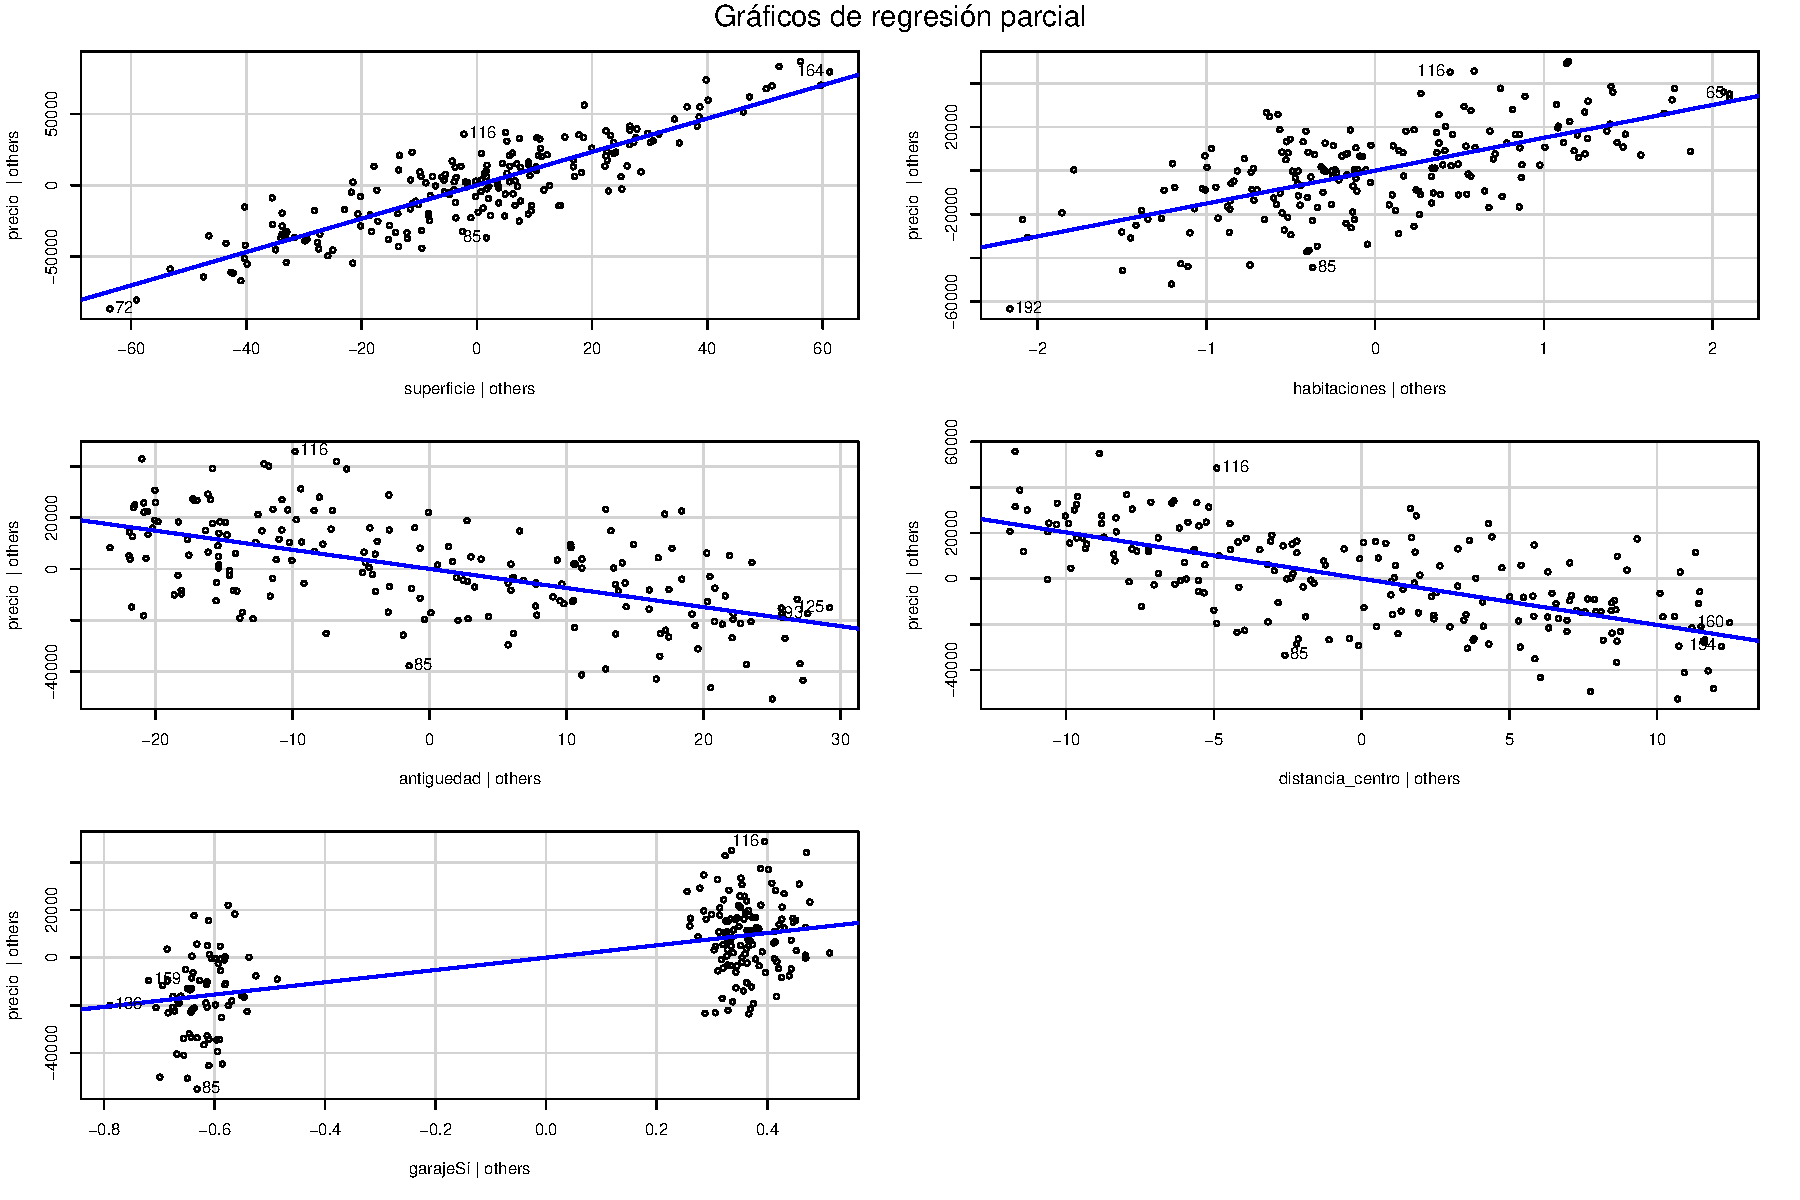
\includegraphics[keepaspectratio]{tema2_files/figure-pdf/graficos-regresion-parcial-1.pdf}}

\textbf{¿Qué vemos en cada gráfico?}

\begin{itemize}
\tightlist
\item
  \textbf{Eje X}: Residuos de la regresión de \(X_j\) vs.~todos los
  demás predictores
\item
  \textbf{Eje Y}: Residuos de la regresión de \(Y\) vs.~todos los demás
  predictores (excepto \(X_j\))
\item
  \textbf{Pendiente}: Es exactamente el coeficiente \(\hat{\beta}_j\)
  del modelo múltiple
\item
  \textbf{Puntos alejados}: Observaciones influyentes para ese
  coeficiente específico
\end{itemize}

\textbf{Interpretación práctica:} - Una relación lineal clara confirma
la validez del modelo - Puntos muy alejados de la línea pueden ser
observaciones influyentes - Patrones curvos sugieren no-linealidad en
esa variable específica

\end{tcolorbox}

\bookmarksetup{startatroot}

\chapter{Ingeniería de características: transformaciones de variables e
interacciones}\label{sec-tema3}

En la práctica del análisis de datos, los datos en su estado bruto
raramente están en la forma óptima para el modelado estadístico. La
\textbf{ingeniería de características} es el proceso fundamental que
transforma, combina y crea variables para maximizar la capacidad
predictiva y la interpretabilidad de nuestros modelos (Kuhn and Johnson
2019; Zheng and Casari 2018).

Este proceso abarca tres áreas principales que exploraremos en
profundidad:

\textbf{Transformaciones de variables}: Las transformaciones matemáticas
nos permiten abordar múltiples problemas simultaneamente: linearizar
relaciones no lineales, estabilizar la varianza (heterocedasticidad),
aproximar la distribución de los errores a la normalidad, y reducir la
influencia de valores atípicos. Dominar cuándo y cómo aplicar
transformaciones logarítmicas, potenciales, Box-Cox o Yeo-Johnson es
fundamental para optimizar nuestros modelos (Box and Cox 1964; Yeo and
Johnson 2000).

\textbf{Tratamiento de variables categóricas}: Las variables categóricas
requieren estrategias específicas de codificación que preserven la
información relevante sin introducir supuestos erróneos. La elección
entre codificación ordinal, one-hot encoding, o técnicas más avanzadas
puede impactar significativamente el rendimiento del modelo (Potdar,
Pardawala, and Pai 2017).

\textbf{Interacciones entre variables}: Las interacciones capturan cómo
el efecto de una variable puede cambiar según el nivel de otra variable,
revelando patrones que los efectos principales por sí solos no pueden
detectar. Comprender los diferentes tipos de interacciones y sus
aplicaciones es clave para modelar relaciones complejas en el mundo real
(Jaccard and Turrisi 2003).

\begin{tcolorbox}[enhanced jigsaw, leftrule=.75mm, breakable, colbacktitle=quarto-callout-important-color!10!white, bottomrule=.15mm, colframe=quarto-callout-important-color-frame, toprule=.15mm, colback=white, coltitle=black, bottomtitle=1mm, left=2mm, title=\textcolor{quarto-callout-important-color}{\faExclamation}\hspace{0.5em}{Objetivos de aprendizaje}, opacityback=0, arc=.35mm, opacitybacktitle=0.6, toptitle=1mm, titlerule=0mm, rightrule=.15mm]

Al finalizar este capítulo, serás capaz de:

\begin{enumerate}
\def\labelenumi{\arabic{enumi}.}
\tightlist
\item
  \textbf{Identificar cuándo aplicar transformaciones} específicas según
  el problema: linearización, heterocedasticidad, normalidad, o
  atípicos.
\item
  \textbf{Aplicar transformaciones clásicas} (logarítmica, potencial,
  inversa) y \textbf{avanzadas} (Box-Cox, Yeo-Johnson) de manera
  apropiada.
\item
  \textbf{Interpretar modelos transformados}, comprendiendo cómo cambia
  el significado de los coeficientes después de la transformación.
\item
  \textbf{Codificar variables categóricas} using ordinal encoding y
  one-hot encoding según la naturaleza de las categorías.
\item
  \textbf{Crear e interpretar términos de interacción} entre variables
  continuas, categóricas, y mixtas.
\item
  \textbf{Aplicar ingeniería de características} para crear nuevas
  variables predictivas mediante combinaciones, ratios y
  transformaciones.
\end{enumerate}

\end{tcolorbox}

\section{Transformaciones de variables: propósitos y
aplicaciones}\label{transformaciones-de-variables-propuxf3sitos-y-aplicaciones}

En el análisis de datos y la construcción de modelos estadísticos, los
datos en su forma original no siempre están preparados para obtener el
máximo rendimiento de nuestros modelos. Las \textbf{transformaciones de
variables} son herramientas fundamentales que nos permiten modificar la
estructura matemática de nuestros datos para abordar problemas
específicos y mejorar significativamente el ajuste del modelo (Box and
Cox 1964; Carroll and Ruppert 1988).

La clave del éxito en las transformaciones está en diagnosticar
correctamente el problema que enfrentamos y seleccionar la
transformación apropiada. Cada transformación tiene propósitos
específicos y consecuencias interpretativas que debemos comprender
profundamente.

\subsection{Diagnóstico: ¿Cuándo
transformar?}\label{diagnuxf3stico-cuuxe1ndo-transformar}

El arte de las transformaciones no está en aplicarlas
indiscriminadamente, sino en diagnosticar correctamente cuál es el
problema que enfrentamos y seleccionar la transformación más apropiada
para resolverlo. Un diagnóstico erróneo puede llevarnos a aplicar una
transformación innecesaria o, peor aún, contraproducente que distorsione
las relaciones reales en los datos.

La práctica común de ``probar transformaciones hasta que mejore el
ajuste'' es metodológicamente peligrosa. Este enfoque de transformación
por ensayo y error puede llevarnos a:

\begin{itemize}
\tightlist
\item
  \textbf{Sobreajuste}: Optimizar el modelo para los datos específicos
  que tenemos, perdiendo capacidad de generalización.
\item
  \textbf{Pérdida de interpretabilidad}: Aplicar transformaciones
  complejas sin comprender su significado teórico.
\item
  \textbf{Violación de supuestos}: Resolver un problema creando otros
  nuevos (ej. transformar para normalidad pero introducir
  heterocedasticidad).
\item
  \textbf{Sesgo de selección}: Elegir la transformación que da los
  ``mejores'' resultados sin justificación teórica.
\end{itemize}

El proceso de diagnóstico debe ser \textbf{sistemático y basado en
evidencia visual y estadística}. No basta con aplicar transformaciones
porque ``mejoran el R²''; debemos entender qué problema específico
estamos resolviendo y cómo la transformación aborda ese problema desde
una perspectiva teórica sólida.

Un enfoque metodológicamente sólido sigue estos principios:

\begin{enumerate}
\def\labelenumi{\arabic{enumi}.}
\item
  \textbf{Diagnóstico previo}: Identificar problemas específicos
  mediante análisis visual y tests estadísticos antes de decidir
  transformar.
\item
  \textbf{Justificación teórica}: Cada transformación debe tener una
  base conceptual sólida. Por ejemplo, usar logaritmos para relaciones
  multiplicativas o raíz cuadrada para estabilizar varianza Poisson.
\item
  \textbf{Evaluación integral}: No solo considerar el ajuste
  estadístico, sino también la interpretabilidad, robustez y
  generalización del modelo transformado.
\item
  \textbf{Validación posterior}: Verificar que la transformación
  realmente resuelve el problema identificado sin crear nuevos
  problemas.
\item
  \textbf{Parsimonia}: Preferir la transformación más simple que
  resuelva efectivamente el problema (principio de Occam aplicado a
  transformaciones).
\end{enumerate}

\begin{tcolorbox}[enhanced jigsaw, leftrule=.75mm, breakable, colbacktitle=quarto-callout-note-color!10!white, bottomrule=.15mm, colframe=quarto-callout-note-color-frame, toprule=.15mm, colback=white, coltitle=black, bottomtitle=1mm, left=2mm, title=\textcolor{quarto-callout-note-color}{\faInfo}\hspace{0.5em}{Recordatorio: Diagnóstico de problemas en regresión lineal}, opacityback=0, arc=.35mm, opacitybacktitle=0.6, toptitle=1mm, titlerule=0mm, rightrule=.15mm]

\textbf{Identificación de no linealidad:} La no linealidad es uno de los
problemas más comunes que enfrentamos en el modelado. \emph{Diagnóstico
visual:} gráficos de dispersión (Y vs.~X), gráficos de componente +
residuo (CPR plots), análisis de residuos vs.~valores ajustados.
\emph{Diagnóstico estadístico:} Test de Ramsey RESET que evalúa si
potencias de los valores ajustados mejoran significativamente el modelo.

\textbf{Detección de heterocedasticidad:} La heterocedasticidad
(varianza no constante) viola supuestos fundamentales de la regresión
lineal y sesga las inferencias estadísticas. \emph{Diagnóstico visual:}
gráfico de residuos vs.~valores ajustados (patrón ``embudo''), gráfico
Scale-Location, residuos vs.~variables predictoras individuales.
\emph{Diagnóstico estadístico:} Test de Breusch-Pagan (el más utilizado)
y Test de White (más general).

\textbf{Evaluación de normalidad de residuos:} Aunque la normalidad no
es crítica para estimación de coeficientes, sí es importante para
inferencia estadística. \emph{Diagnóstico visual:} histograma de
residuos, QQ-plot de residuos. \emph{Diagnóstico estadístico:} Test de
Shapiro-Wilk (muestras pequeñas n\textless50) y Test de Jarque-Bera.

\textbf{Detección de outliers y observaciones influyentes:} Es
fundamental distinguir entre outliers (valores extremos en Y) y
observaciones influyentes (impacto en coeficientes). \emph{Outliers:}
boxplot de variable respuesta, residuos estudentizados, criterios
\textbar t\(_i\)\textbar{} \textgreater{} 2. \emph{Observaciones
influyentes:} análisis de leverage, distancia de Cook, DFBETAS, DFFITS,
con criterios específicos como h\(_i\) \textgreater{} 2p/n y D\(_i\)
\textgreater{} 4/n.~Las observaciones se clasifican en: normales,
outliers no influyentes, influyentes sin ser outliers, y outliers
influyentes.

\end{tcolorbox}

\section{Escalado y normalización: preparando variables para el
análisis}\label{escalado-y-normalizaciuxf3n-preparando-variables-para-el-anuxe1lisis}

Antes de aplicar transformaciones complejas, es fundamental asegurar que
nuestras variables estén en escalas comparables. Aunque la regresión
lineal ordinaria no requiere estrictamente el escalado de variables para
obtener estimadores insesgados, el escalado se vuelve crítico para la
interpretación y esencial en métodos avanzados de modelado.

En regresión múltiple, los coeficientes representan el cambio en Y por
unidad de cambio en cada variable predictora. Cuando las variables
tienen escalas muy diferentes, los coeficientes pierden comparabilidad
directa. Una variable medida en miles de euros tendrá coeficientes
numéricamente pequeños, mientras que una variable medida en porcentajes
tendrá coeficientes grandes, independientemente de su importancia real
en el modelo.

Esta disparidad de escalas genera problemas interpretativos
fundamentales: comparar la ``importancia'' relativa de las variables se
vuelve imposible basándose únicamente en la magnitud de los
coeficientes. El escalado resuelve este problema permitiendo que los
coeficientes estandarizados (beta coefficients) representen cambios en
desviaciones estándar, facilitando comparaciones directas entre
predictores y proporcionando una base sólida para evaluar la importancia
relativa de cada variable.

\begin{tcolorbox}[enhanced jigsaw, leftrule=.75mm, breakable, colbacktitle=quarto-callout-note-color!10!white, bottomrule=.15mm, colframe=quarto-callout-note-color-frame, toprule=.15mm, colback=white, coltitle=black, bottomtitle=1mm, left=2mm, title=\textcolor{quarto-callout-note-color}{\faInfo}\hspace{0.5em}{Escalado en métodos de regularización}, opacityback=0, arc=.35mm, opacitybacktitle=0.6, toptitle=1mm, titlerule=0mm, rightrule=.15mm]

\textbf{En regresión con regularización (Ridge, Lasso)}, el problema se
agrava dramáticamente. Las penalizaciones L1 y L2 afectan
\textbf{desproporcionadamente} a variables con escalas grandes, llevando
a regularización injusta donde variables con unidades grandes son
penalizadas más severamente que variables con unidades pequeñas,
independientemente de su relevancia predictiva. Esto puede resultar en
selección de variables sesgada y estimadores subóptimos. Este tema se
desarrollará en profundidad en el siguiente capítulo sobre métodos de
regularización.

\end{tcolorbox}

El escalado no es solo una cuestión técnica, sino una decisión
metodológica que afecta directamente la interpretación y validez de
nuestros resultados. La elección entre estandarización, normalización
min-max, o escalado robusto debe basarse en las características de los
datos y los objetivos del análisis, considerando siempre el impacto en
la interpretabilidad de los resultados finales.

\subsection{Estandarización (Z-Score)}\label{estandarizaciuxf3n-z-score}

La \textbf{estandarización} es la técnica de escalado más utilizada en
estadística. Transforma cada variable para que tenga media cero y
desviación estándar uno, preservando la forma de la distribución
original.

\[X_{\text{estandarizado}} = \frac{X - \bar{X}}{\sigma_X}\]

\textbf{Propiedades de la estandarización:}

\begin{itemize}
\tightlist
\item
  \textbf{Preserva la forma de la distribución}: Si X era normal, X
  estandarizado también lo será.
\item
  \textbf{Facilita la comparación}: Los coeficientes en regresión
  múltiple se vuelven comparables.
\item
  \textbf{Robusta ante outliers moderados}: La media y desviación
  estándar son menos sensibles que min-max a valores extremos.
\end{itemize}

\textbf{Cuándo usar estandarización:}

\begin{itemize}
\tightlist
\item
  Variables con distribuciones aproximadamente normales.
\item
  Cuando necesitamos preservar la información sobre la variabilidad
  relativa.
\item
  En regresión múltiple para comparar la importancia relativa de las
  variables.
\item
  Como paso previo a técnicas multivariantes (PCA, análisis
  discriminante).
\end{itemize}

\subsection{Normalización Min-Max}\label{normalizaciuxf3n-min-max}

La \textbf{normalización Min-Max} escala las variables a un rango
específico, típicamente {[}0,1{]}, preservando las relaciones relativas
entre los valores.

\[X_{\text{normalizado}} = \frac{X - X_{\text{min}}}{X_{\text{max}} - X_{\text{min}}}\]

\textbf{Propiedades de la normalización Min-Max:}

\begin{itemize}
\tightlist
\item
  \textbf{Rango acotado}: Todas las variables transformadas tienen el
  mismo rango {[}0,1{]}.
\item
  \textbf{Preserva relaciones}: Las distancias relativas entre
  observaciones se mantienen.
\item
  \textbf{Interpretación intuitiva}: 0 representa el mínimo observado, 1
  el máximo observado.
\end{itemize}

\textbf{Cuándo usar normalización Min-Max:}

\begin{itemize}
\tightlist
\item
  Cuando necesitamos un rango específico (ej. entradas de redes
  neuronales).
\item
  Variables con distribuciones uniformes o sin outliers extremos.
\item
  Cuando la interpretación en términos de mínimo-máximo es relevante.
\item
  En algoritmos que requieren entradas en {[}0,1{]} (algunos métodos de
  ensemble).
\end{itemize}

\textbf{Limitaciones:}

\begin{itemize}
\tightlist
\item
  \textbf{Muy sensible a outliers}: Un solo valor extremo puede
  comprimir toda la distribución.
\item
  \textbf{No preserva la normalidad}: Una distribución normal se vuelve
  uniforme tras Min-Max.
\end{itemize}

\subsection{Escalado robusto}\label{escalado-robusto}

Para datos con outliers significativos, el escalado robusto utiliza la
mediana y el rango intercuartílico (IQR) en lugar de la media y
desviación estándar:

\[X_{\text{robusto}} = \frac{X - \text{mediana}(X)}{\text{IQR}(X)}\]

Este método es menos sensible a valores extremos y preserva mejor la
estructura de los datos en presencia de outliers.

\begin{tcolorbox}[enhanced jigsaw, leftrule=.75mm, breakable, colbacktitle=quarto-callout-tip-color!10!white, bottomrule=.15mm, colframe=quarto-callout-tip-color-frame, toprule=.15mm, colback=white, coltitle=black, bottomtitle=1mm, left=2mm, title=\textcolor{quarto-callout-tip-color}{\faLightbulb}\hspace{0.5em}{Ejemplo comparativo: Escalado de variables}, opacityback=0, arc=.35mm, opacitybacktitle=0.6, toptitle=1mm, titlerule=0mm, rightrule=.15mm]

\begin{Shaded}
\begin{Highlighting}[]
\CommentTok{\# Generar datos de ejemplo con diferentes escalas}
\FunctionTok{set.seed}\NormalTok{(}\DecValTok{123}\NormalTok{)}
\NormalTok{n }\OtherTok{\textless{}{-}} \DecValTok{100}

\CommentTok{\# Variable de ejemplo: Ingresos en miles de euros}
\NormalTok{ingresos }\OtherTok{\textless{}{-}} \FunctionTok{rnorm}\NormalTok{(n, }\AttributeTok{mean =} \DecValTok{50}\NormalTok{, }\AttributeTok{sd =} \DecValTok{15}\NormalTok{)}

\CommentTok{\# Aplicar diferentes transformaciones}
\NormalTok{ingresos\_std }\OtherTok{\textless{}{-}} \FunctionTok{scale}\NormalTok{(ingresos)[,}\DecValTok{1}\NormalTok{]  }\CommentTok{\# Estandarización}
\NormalTok{ingresos\_norm }\OtherTok{\textless{}{-}}\NormalTok{ (ingresos }\SpecialCharTok{{-}} \FunctionTok{min}\NormalTok{(ingresos)) }\SpecialCharTok{/}\NormalTok{ (}\FunctionTok{max}\NormalTok{(ingresos) }\SpecialCharTok{{-}} \FunctionTok{min}\NormalTok{(ingresos))  }\CommentTok{\# Min{-}Max}
\NormalTok{ingresos\_robust }\OtherTok{\textless{}{-}}\NormalTok{ (ingresos }\SpecialCharTok{{-}} \FunctionTok{median}\NormalTok{(ingresos)) }\SpecialCharTok{/} \FunctionTok{IQR}\NormalTok{(ingresos)  }\CommentTok{\# Robusto}

\CommentTok{\# Crear tabla comparativa}
\FunctionTok{library}\NormalTok{(knitr)}
\NormalTok{tabla\_escalado }\OtherTok{\textless{}{-}} \FunctionTok{data.frame}\NormalTok{(}
\NormalTok{  Método }\OtherTok{=} \FunctionTok{c}\NormalTok{(}\StringTok{"Original"}\NormalTok{, }\StringTok{"Estandarización"}\NormalTok{, }\StringTok{"Min{-}Max"}\NormalTok{, }\StringTok{"Escalado Robusto"}\NormalTok{),}
  \AttributeTok{Media =} \FunctionTok{round}\NormalTok{(}\FunctionTok{c}\NormalTok{(}\FunctionTok{mean}\NormalTok{(ingresos), }\FunctionTok{mean}\NormalTok{(ingresos\_std), }\FunctionTok{mean}\NormalTok{(ingresos\_norm), }\FunctionTok{median}\NormalTok{(ingresos\_robust)), }\DecValTok{3}\NormalTok{),}
\NormalTok{  Desviación }\OtherTok{=} \FunctionTok{round}\NormalTok{(}\FunctionTok{c}\NormalTok{(}\FunctionTok{sd}\NormalTok{(ingresos), }\FunctionTok{sd}\NormalTok{(ingresos\_std), }\FunctionTok{sd}\NormalTok{(ingresos\_norm), }\FunctionTok{mad}\NormalTok{(ingresos\_robust)), }\DecValTok{3}\NormalTok{),}
\NormalTok{  Mínimo }\OtherTok{=} \FunctionTok{round}\NormalTok{(}\FunctionTok{c}\NormalTok{(}\FunctionTok{min}\NormalTok{(ingresos), }\FunctionTok{min}\NormalTok{(ingresos\_std), }\FunctionTok{min}\NormalTok{(ingresos\_norm), }\FunctionTok{min}\NormalTok{(ingresos\_robust)), }\DecValTok{3}\NormalTok{),}
\NormalTok{  Máximo }\OtherTok{=} \FunctionTok{round}\NormalTok{(}\FunctionTok{c}\NormalTok{(}\FunctionTok{max}\NormalTok{(ingresos), }\FunctionTok{max}\NormalTok{(ingresos\_std), }\FunctionTok{max}\NormalTok{(ingresos\_norm), }\FunctionTok{max}\NormalTok{(ingresos\_robust)), }\DecValTok{3}\NormalTok{),}
  \AttributeTok{Rango =} \FunctionTok{round}\NormalTok{(}\FunctionTok{c}\NormalTok{(}
    \FunctionTok{max}\NormalTok{(ingresos) }\SpecialCharTok{{-}} \FunctionTok{min}\NormalTok{(ingresos),}
    \FunctionTok{max}\NormalTok{(ingresos\_std) }\SpecialCharTok{{-}} \FunctionTok{min}\NormalTok{(ingresos\_std),}
    \FunctionTok{max}\NormalTok{(ingresos\_norm) }\SpecialCharTok{{-}} \FunctionTok{min}\NormalTok{(ingresos\_norm),}
    \FunctionTok{max}\NormalTok{(ingresos\_robust) }\SpecialCharTok{{-}} \FunctionTok{min}\NormalTok{(ingresos\_robust)}
\NormalTok{  ), }\DecValTok{3}\NormalTok{)}
\NormalTok{)}

\FunctionTok{kable}\NormalTok{(tabla\_escalado, }\AttributeTok{caption =} \StringTok{"Comparación de métodos de escalado en variable Ingresos"}\NormalTok{)}
\end{Highlighting}
\end{Shaded}

\begin{longtable}[]{@{}lrrrrr@{}}
\caption{Comparación de métodos de escalado en variable
Ingresos}\tabularnewline
\toprule\noalign{}
Método & Media & Desviación & Mínimo & Máximo & Rango \\
\midrule\noalign{}
\endfirsthead
\toprule\noalign{}
Método & Media & Desviación & Mínimo & Máximo & Rango \\
\midrule\noalign{}
\endhead
\bottomrule\noalign{}
\endlastfoot
Original & 51.356 & 13.692 & 15.362 & 82.810 & 67.448 \\
Estandarización & 0.000 & 1.000 & -2.629 & 2.297 & 4.926 \\
Min-Max & 0.534 & 0.203 & 0.000 & 1.000 & 1.000 \\
Escalado Robusto & 0.000 & 0.750 & -2.000 & 1.793 & 3.792 \\
\end{longtable}

\textbf{Interpretación de los resultados:}

\begin{itemize}
\tightlist
\item
  \textbf{Original}: Ingresos en miles de euros con gran variabilidad
  (SD ≈ 15)
\item
  \textbf{Estandarización}: Media = 0, SD = 1, preservando la forma de
  la distribución
\item
  \textbf{Min-Max}: Valores acotados entre {[}0,1{]}, comprimiendo toda
  la variabilidad en este rango
\item
  \textbf{Escalado Robusto}: Centrado en la mediana, menos sensible a
  valores extremos
\end{itemize}

Cada método transforma los datos de manera diferente según el objetivo:
comparabilidad (estandarización), rango específico (min-max), o robustez
ante outliers (robusto).

\end{tcolorbox}

\begin{tcolorbox}[enhanced jigsaw, leftrule=.75mm, breakable, colbacktitle=quarto-callout-tip-color!10!white, bottomrule=.15mm, colframe=quarto-callout-tip-color-frame, toprule=.15mm, colback=white, coltitle=black, bottomtitle=1mm, left=2mm, title=\textcolor{quarto-callout-tip-color}{\faLightbulb}\hspace{0.5em}{Ejemplo con outliers: Escalado robusto}, opacityback=0, arc=.35mm, opacitybacktitle=0.6, toptitle=1mm, titlerule=0mm, rightrule=.15mm]

\begin{Shaded}
\begin{Highlighting}[]
\CommentTok{\# Datos con outliers}
\FunctionTok{set.seed}\NormalTok{(}\DecValTok{456}\NormalTok{)}
\NormalTok{datos\_normales }\OtherTok{\textless{}{-}} \FunctionTok{rnorm}\NormalTok{(}\DecValTok{95}\NormalTok{, }\DecValTok{10}\NormalTok{, }\DecValTok{2}\NormalTok{)}
\NormalTok{outliers }\OtherTok{\textless{}{-}} \FunctionTok{c}\NormalTok{(}\DecValTok{25}\NormalTok{, }\DecValTok{30}\NormalTok{, }\DecValTok{35}\NormalTok{, }\DecValTok{40}\NormalTok{, }\DecValTok{45}\NormalTok{)}
\NormalTok{datos\_outliers }\OtherTok{\textless{}{-}} \FunctionTok{c}\NormalTok{(datos\_normales, outliers)}

\CommentTok{\# Aplicar diferentes métodos de escalado}
\NormalTok{std\_clasica }\OtherTok{\textless{}{-}} \FunctionTok{scale}\NormalTok{(datos\_outliers)[,}\DecValTok{1}\NormalTok{]}
\NormalTok{norm\_minmax }\OtherTok{\textless{}{-}}\NormalTok{ (datos\_outliers }\SpecialCharTok{{-}} \FunctionTok{min}\NormalTok{(datos\_outliers)) }\SpecialCharTok{/}\NormalTok{ (}\FunctionTok{max}\NormalTok{(datos\_outliers) }\SpecialCharTok{{-}} \FunctionTok{min}\NormalTok{(datos\_outliers))}
\NormalTok{escalado\_robusto }\OtherTok{\textless{}{-}}\NormalTok{ (datos\_outliers }\SpecialCharTok{{-}} \FunctionTok{median}\NormalTok{(datos\_outliers)) }\SpecialCharTok{/} \FunctionTok{IQR}\NormalTok{(datos\_outliers)}

\CommentTok{\# Crear tabla comparativa}
\FunctionTok{library}\NormalTok{(knitr)}
\NormalTok{tabla\_outliers }\OtherTok{\textless{}{-}} \FunctionTok{data.frame}\NormalTok{(}
\NormalTok{  Método }\OtherTok{=} \FunctionTok{c}\NormalTok{(}\StringTok{"Original"}\NormalTok{, }\StringTok{"Estandarización"}\NormalTok{, }\StringTok{"Min{-}Max"}\NormalTok{, }\StringTok{"Escalado Robusto"}\NormalTok{),}
  \AttributeTok{Media\_Mediana =} \FunctionTok{round}\NormalTok{(}\FunctionTok{c}\NormalTok{(}\FunctionTok{mean}\NormalTok{(datos\_outliers), }\FunctionTok{mean}\NormalTok{(std\_clasica), }\FunctionTok{mean}\NormalTok{(norm\_minmax), }\FunctionTok{median}\NormalTok{(escalado\_robusto)), }\DecValTok{3}\NormalTok{),}
\NormalTok{  Desviación }\OtherTok{=} \FunctionTok{round}\NormalTok{(}\FunctionTok{c}\NormalTok{(}\FunctionTok{sd}\NormalTok{(datos\_outliers), }\FunctionTok{sd}\NormalTok{(std\_clasica), }\FunctionTok{sd}\NormalTok{(norm\_minmax), }\FunctionTok{mad}\NormalTok{(escalado\_robusto)), }\DecValTok{3}\NormalTok{),}
\NormalTok{  Mínimo }\OtherTok{=} \FunctionTok{round}\NormalTok{(}\FunctionTok{c}\NormalTok{(}\FunctionTok{min}\NormalTok{(datos\_outliers), }\FunctionTok{min}\NormalTok{(std\_clasica), }\FunctionTok{min}\NormalTok{(norm\_minmax), }\FunctionTok{min}\NormalTok{(escalado\_robusto)), }\DecValTok{3}\NormalTok{),}
\NormalTok{  Máximo }\OtherTok{=} \FunctionTok{round}\NormalTok{(}\FunctionTok{c}\NormalTok{(}\FunctionTok{max}\NormalTok{(datos\_outliers), }\FunctionTok{max}\NormalTok{(std\_clasica), }\FunctionTok{max}\NormalTok{(norm\_minmax), }\FunctionTok{max}\NormalTok{(escalado\_robusto)), }\DecValTok{3}\NormalTok{),}
  \AttributeTok{Q25\_Q75 =} \FunctionTok{c}\NormalTok{(}
    \FunctionTok{paste}\NormalTok{(}\FunctionTok{round}\NormalTok{(}\FunctionTok{quantile}\NormalTok{(datos\_outliers, }\FunctionTok{c}\NormalTok{(}\FloatTok{0.25}\NormalTok{, }\FloatTok{0.75}\NormalTok{)), }\DecValTok{2}\NormalTok{), }\AttributeTok{collapse =} \StringTok{" {-} "}\NormalTok{),}
    \FunctionTok{paste}\NormalTok{(}\FunctionTok{round}\NormalTok{(}\FunctionTok{quantile}\NormalTok{(std\_clasica, }\FunctionTok{c}\NormalTok{(}\FloatTok{0.25}\NormalTok{, }\FloatTok{0.75}\NormalTok{)), }\DecValTok{2}\NormalTok{), }\AttributeTok{collapse =} \StringTok{" {-} "}\NormalTok{),}
    \FunctionTok{paste}\NormalTok{(}\FunctionTok{round}\NormalTok{(}\FunctionTok{quantile}\NormalTok{(norm\_minmax, }\FunctionTok{c}\NormalTok{(}\FloatTok{0.25}\NormalTok{, }\FloatTok{0.75}\NormalTok{)), }\DecValTok{2}\NormalTok{), }\AttributeTok{collapse =} \StringTok{" {-} "}\NormalTok{),}
    \FunctionTok{paste}\NormalTok{(}\FunctionTok{round}\NormalTok{(}\FunctionTok{quantile}\NormalTok{(escalado\_robusto, }\FunctionTok{c}\NormalTok{(}\FloatTok{0.25}\NormalTok{, }\FloatTok{0.75}\NormalTok{)), }\DecValTok{2}\NormalTok{), }\AttributeTok{collapse =} \StringTok{" {-} "}\NormalTok{)}
\NormalTok{  )}
\NormalTok{)}

\FunctionTok{kable}\NormalTok{(tabla\_outliers, }\AttributeTok{caption =} \StringTok{"Comparación de métodos de escalado con outliers presentes"}\NormalTok{)}
\end{Highlighting}
\end{Shaded}

\begin{longtable}[]{@{}
  >{\raggedright\arraybackslash}p{(\linewidth - 10\tabcolsep) * \real{0.2464}}
  >{\raggedleft\arraybackslash}p{(\linewidth - 10\tabcolsep) * \real{0.2029}}
  >{\raggedleft\arraybackslash}p{(\linewidth - 10\tabcolsep) * \real{0.1594}}
  >{\raggedleft\arraybackslash}p{(\linewidth - 10\tabcolsep) * \real{0.1014}}
  >{\raggedleft\arraybackslash}p{(\linewidth - 10\tabcolsep) * \real{0.1014}}
  >{\raggedright\arraybackslash}p{(\linewidth - 10\tabcolsep) * \real{0.1884}}@{}}
\caption{Comparación de métodos de escalado con outliers
presentes}\tabularnewline
\toprule\noalign{}
\begin{minipage}[b]{\linewidth}\raggedright
Método
\end{minipage} & \begin{minipage}[b]{\linewidth}\raggedleft
Media\_Mediana
\end{minipage} & \begin{minipage}[b]{\linewidth}\raggedleft
Desviación
\end{minipage} & \begin{minipage}[b]{\linewidth}\raggedleft
Mínimo
\end{minipage} & \begin{minipage}[b]{\linewidth}\raggedleft
Máximo
\end{minipage} & \begin{minipage}[b]{\linewidth}\raggedright
Q25\_Q75
\end{minipage} \\
\midrule\noalign{}
\endfirsthead
\toprule\noalign{}
\begin{minipage}[b]{\linewidth}\raggedright
Método
\end{minipage} & \begin{minipage}[b]{\linewidth}\raggedleft
Media\_Mediana
\end{minipage} & \begin{minipage}[b]{\linewidth}\raggedleft
Desviación
\end{minipage} & \begin{minipage}[b]{\linewidth}\raggedleft
Mínimo
\end{minipage} & \begin{minipage}[b]{\linewidth}\raggedleft
Máximo
\end{minipage} & \begin{minipage}[b]{\linewidth}\raggedright
Q25\_Q75
\end{minipage} \\
\midrule\noalign{}
\endhead
\bottomrule\noalign{}
\endlastfoot
Original & 11.447 & 5.996 & 5.491 & 45.000 & 8.93 - 11.81 \\
Estandarización & 0.000 & 1.000 & -0.993 & 5.595 & -0.42 - 0.06 \\
Min-Max & 0.151 & 0.152 & 0.000 & 1.000 & 0.09 - 0.16 \\
Escalado Robusto & 0.000 & 0.778 & -1.654 & 12.108 & -0.45 - 0.55 \\
\end{longtable}

\textbf{Análisis del impacto de outliers:}

\begin{itemize}
\tightlist
\item
  \textbf{Datos originales}: Los outliers extienden el rango de
  \textasciitilde6-14 a 6-45, distorsionando las medidas centrales
\item
  \textbf{Estandarización}: Afectada por outliers en media y desviación
  estándar, resultando en distribución asimétrica
\item
  \textbf{Min-Max}: Extremadamente sensible. Los datos normales quedan
  comprimidos en un rango muy pequeño (\textasciitilde0.0-0.2)
\item
  \textbf{Escalado robusto}: Mantiene mejor las proporciones de la
  distribución central, minimizando la influencia de valores extremos
\end{itemize}

\textbf{Conclusión}: El escalado robusto es superior cuando hay
outliers, preservando la estructura de la mayoría de observaciones.

\end{tcolorbox}

\section{Catálogo de transformaciones según el
propósito}\label{catuxe1logo-de-transformaciones-seguxfan-el-propuxf3sito}

Una vez realizado el diagnóstico, debemos seleccionar la transformación
más apropiada. Cada transformación tiene propósitos específicos y
efectos secundarios que debemos considerar. La clave está en entender no
solo qué transformación aplicar, sino por qué esa transformación
específica resuelve nuestro problema.

\subsection{Transformaciones para linearizar
relaciones}\label{transformaciones-para-linearizar-relaciones}

Muchas relaciones en el mundo real no son lineales, pero pueden
linearizarse mediante transformaciones apropiadas. La linearización no
solo mejora el ajuste del modelo, sino que también facilita la
interpretación y cumple con los supuestos de la regresión lineal.

\subsubsection{Transformación
logarítmica}\label{transformaciuxf3n-logaruxedtmica}

La transformación logarítmica es probablemente la más utilizada en
estadística aplicada debido a su versatilidad y propiedades
interpretativas únicas.

\textbf{Cuándo utilizarla:}

\begin{itemize}
\tightlist
\item
  Relaciones exponenciales: Cuando Y crece exponencialmente respecto a
  X, \(Y = ae^{bX}\) se lineariza como \(\log(Y) = \log(a) + bX\)
\item
  Relaciones multiplicativas: En modelos donde los efectos se combinan
  multiplicativamente
\item
  Procesos de crecimiento proporcional: Donde la tasa de cambio es
  proporcional al nivel actual
\item
  Variables con crecimiento acelerado: Ingresos, precios, donde cada
  unidad adicional tiene impacto decreciente
\end{itemize}

\textbf{Patrones de identificación:}

\begin{itemize}
\tightlist
\item
  Curva cóncava que se aplana hacia la derecha (rendimientos
  decrecientes)
\item
  Relación donde duplicar X no duplica Y, sino que el efecto se atenúa
\item
  Heterocedasticidad donde la varianza aumenta con el nivel de Y
\end{itemize}

\textbf{Aplicaciones matemáticas:}

\begin{itemize}
\tightlist
\item
  \(Y' = \log(Y)\): Lineariza relaciones exponenciales en Y
\item
  \(X' = \log(X)\): Lineariza relaciones de potencia en X\\
\item
  \(\log(Y) = a + b\log(X)\): Modelo log-log que produce elasticidades
  constantes
\end{itemize}

\textbf{Interpretación especial:} En modelos log-lineales y log-log, los
coeficientes tienen interpretaciones económicas directas. En el modelo
log-lineal \(\log(Y) = a + bX\), el coeficiente b representa el cambio
porcentual en Y por unidad de cambio en X. En el modelo log-log
\(\log(Y) = a + b\log(X)\), b es la elasticidad.

\textbf{Casos típicos:} Economía (relaciones ingreso-consumo, funciones
de producción), biología (crecimiento poblacional, relaciones
alométricas), finanzas (rendimientos de inversión).

\subsubsection{Transformación de
potencia}\label{transformaciuxf3n-de-potencia}

Las transformaciones de potencia son fundamentales cuando trabajamos con
leyes físicas o relaciones alométricas donde esperamos relaciones del
tipo \(Y = aX^b\).

\textbf{Identificación y aplicación:}

\begin{itemize}
\tightlist
\item
  Relaciones curvilíneas que en escala log-log se vuelven lineales
\item
  Método de linearización: tomar logaritmo de ambas variables
  \(\log(Y) = \log(a) + b\log(X)\)
\item
  El exponente b representa la elasticidad o exponente de escalamiento
\end{itemize}

\textbf{Ejemplos clásicos:} Ley de Stevens en psicofísica, relaciones
masa-metabolismo (Ley de Kleiber), economía urbana donde PIB de ciudades
escala con población elevada a una potencia.

\subsection{Transformaciones para estabilizar la
varianza}\label{transformaciones-para-estabilizar-la-varianza}

La heterocedasticidad no solo viola supuestos del modelo, sino que
también indica que diferentes observaciones tienen diferentes niveles de
información. Las transformaciones de varianza estabilizan esta
heterogeneidad.

\subsubsection{Transformación de raíz
cuadrada}\label{transformaciuxf3n-de-rauxedz-cuadrada}

La transformación \(Y' = \sqrt{Y}\) es especialmente útil para datos de
conteo donde la varianza es proporcional a la media, característica
típica de la distribución de Poisson.

\textbf{Fundamento teórico:} En una distribución de Poisson con
parámetro \(\lambda\), tanto la media como la varianza son iguales a
\(\lambda\). La transformación de raíz cuadrada estabiliza la varianza
porque \(\text{Var}(\sqrt{Y}) \approx \frac{1}{4}\) (constante).

\textbf{Cuándo aplicarla:}

\begin{itemize}
\tightlist
\item
  Conteos de eventos: número de defectos, llamadas telefónicas,
  accidentes, ventas por período
\item
  Datos de frecuencia: número de visitas, clicks, transacciones
\item
  Variables discretas con varianza creciente proporcional al nivel
\end{itemize}

\textbf{Patrón de diagnóstico:} Gráfico de residuos con forma de embudo
donde la dispersión aumenta linealmente con la media, y gráfico de
varianza vs.~media de grupos muestra relación lineal.

\textbf{Limitaciones:} Solo apropiada para valores no negativos,
interpretación complicada (unidades en raíz cuadrada), y para conteos
con muchos ceros puede requerir \(\sqrt{Y + c}\).

\subsubsection{Transformación logarítmica para heterocedasticidad
multiplicativa}\label{transformaciuxf3n-logaruxedtmica-para-heterocedasticidad-multiplicativa}

Cuando la varianza es proporcional al cuadrado de la media
(heterocedasticidad multiplicativa), la transformación logarítmica es la
solución natural.

\textbf{Características típicas:}

\begin{itemize}
\tightlist
\item
  Variables monetarias: ingresos, precios, costos donde el error
  relativo es constante
\item
  Porcentajes de crecimiento: donde el error de medición es proporcional
  al nivel
\item
  Procesos multiplicativos: donde los errores se acumulan
  multiplicativamente
\end{itemize}

\textbf{Efectos múltiples:} La transformación logarítmica frecuentemente
resuelve múltiples problemas simultáneamente: lineariza relaciones
exponenciales, estabiliza varianza multiplicativa, reduce el impacto de
outliers extremos, y aproxima distribuciones asimétricas a la
normalidad.

\subsection{Transformaciones para normalizar residuos y controlar
outliers}\label{transformaciones-para-normalizar-residuos-y-controlar-outliers}

Algunas transformaciones son especialmente efectivas para aproximar
distribuciones a la normalidad y reducir la influencia de valores
extremos.

\subsubsection{Transformación inversa}\label{transformaciuxf3n-inversa}

La transformación inversa \(Y' = \frac{1}{Y}\) o \(X' = \frac{1}{X}\) es
útil para relaciones hiperbólicas y distribuciones con colas pesadas
hacia la derecha.

\textbf{Identificación matemática:}

\begin{itemize}
\tightlist
\item
  Relación hiperbólica: \(Y = \frac{a}{X} + b\) se lineariza como
  \(Y = a \cdot \frac{1}{X} + b\)
\item
  Asíntota horizontal: la relación se aproxima a un valor límite cuando
  X aumenta
\end{itemize}

\textbf{Aplicaciones específicas:} Tiempo hasta el evento (con asíntota
natural), tasas de decaimiento, relaciones dosis-respuesta en
farmacología, curvas de demanda con elasticidad precio variable.

\textbf{Efecto en outliers:} La transformación inversa invierte la
escala, comprimiendo fuertemente los valores grandes y expandiendo los
pequeños. Útil para reducir influencia de outliers extremos, pero debe
usarse con precaución ya que amplifica errores en valores pequeños.

\textbf{Consideraciones prácticas:} Solo aplicable a valores
estrictamente positivos (o negativos), los coeficientes representan el
impacto en la escala inversa, y requiere tratamiento especial para
valores cercanos a cero.

\section{Transformación de Box-Cox}\label{transformaciuxf3n-de-box-cox}

La transformación de Box-Cox es un método que optimiza automáticamente
el parámetro de transformación para maximizar la normalidad y
homocedasticidad de los residuos (Box and Cox 1964). En lugar de elegir
manualmente entre transformación logarítmica, raíz cuadrada o inversa,
Box-Cox encuentra el valor \(\lambda\) (lambda) que mejor normaliza los
datos.

\subsection{Definición matemática}\label{definiciuxf3n-matemuxe1tica}

\[Y(\lambda) = \begin{cases}
\frac{Y^\lambda - 1}{\lambda}, & \lambda \neq 0 \\
\log(Y), & \lambda = 0
\end{cases}\]

Los valores especiales de \(\lambda\) corresponden a transformaciones
clásicas:

\begin{itemize}
\tightlist
\item
  \textbf{\(\lambda\) = 1}: Sin transformación (identidad)
\item
  \textbf{\(\lambda\) = 0.5}: Transformación de raíz cuadrada\\
\item
  \textbf{\(\lambda\) = 0}: Transformación logarítmica
\item
  \textbf{\(\lambda\) = -1}: Transformación inversa
\end{itemize}

\subsection{Propósito y ventajas}\label{propuxf3sito-y-ventajas}

\textbf{Para qué sirve Box-Cox:}

\begin{itemize}
\tightlist
\item
  Encuentra automáticamente la transformación óptima sin prueba y error
\item
  Maximiza la verosimilitud del modelo, mejorando simultáneamente
  normalidad y homocedasticidad
\item
  Proporciona un método objetivo para seleccionar la transformación
  apropiada
\item
  Incluye intervalos de confianza para \(\lambda\), permitiendo evaluar
  la incertidumbre de la estimación
\end{itemize}

\textbf{Procedimiento de aplicación:}

\begin{enumerate}
\def\labelenumi{\arabic{enumi}.}
\tightlist
\item
  Se ajusta el modelo original y se calculan los residuos
\item
  Se evalúa la función de verosimilitud para diferentes valores de
  \(\lambda\)
\item
  Se selecciona el \(\lambda\) que maximiza la verosimilitud
\item
  Se aplica la transformación con el \(\lambda\) óptimo encontrado
\end{enumerate}

\subsection{Limitaciones importantes}\label{limitaciones-importantes}

\textbf{Restricción de dominio:} Box-Cox requiere que todos los valores
de Y sean estrictamente positivos. Esta es su limitación más importante,
ya que muchos conjuntos de datos reales incluyen ceros o valores
negativos.

\textbf{Aplicación tradicional:} Se aplica principalmente a la variable
dependiente Y, no a las variables predictoras. Aunque técnicamente es
posible aplicarla a X, la interpretación se complica considerablemente.

\textbf{Interpretación compleja:} Cuando \(\lambda\) no corresponde a
valores ``simples'' (como 0, 0.5, o 1), la interpretación de los
coeficientes se vuelve difícil. Por ejemplo, si \(\lambda\) = 0.37,
¿cómo interpretar un coeficiente en la escala transformada?

\textbf{Dependencia del modelo:} El \(\lambda\) óptimo depende del
modelo específico (predictores incluidos), por lo que cambiar el modelo
puede requerir recalcular la transformación.

\begin{tcolorbox}[enhanced jigsaw, leftrule=.75mm, breakable, colbacktitle=quarto-callout-note-color!10!white, bottomrule=.15mm, colframe=quarto-callout-note-color-frame, toprule=.15mm, colback=white, coltitle=black, bottomtitle=1mm, left=2mm, title=\textcolor{quarto-callout-note-color}{\faInfo}\hspace{0.5em}{Extensión: Transformación de Yeo-Johnson}, opacityback=0, arc=.35mm, opacitybacktitle=0.6, toptitle=1mm, titlerule=0mm, rightrule=.15mm]

La transformación de Yeo-Johnson (Yeo and Johnson 2000) fue desarrollada
específicamente para superar la limitación principal de Box-Cox: la
restricción a valores positivos.

\textbf{Ventajas de Yeo-Johnson sobre Box-Cox:}

\begin{itemize}
\tightlist
\item
  \textbf{Sin restricción de dominio}: Acepta cualquier valor real,
  incluyendo negativos y cero
\item
  \textbf{Preserva el signo}: Los valores negativos permanecen negativos
  tras la transformación
\item
  \textbf{Continuidad}: La transformación es continua en Y = 0, evitando
  discontinuidades
\item
  \textbf{Casos especiales familiares}: Incluye como casos especiales
  todas las transformaciones comunes
\end{itemize}

\textbf{Cuándo usar cada una:}

\begin{itemize}
\tightlist
\item
  \textbf{Box-Cox}: Para datos estrictamente positivos, especialmente
  cuando se busca comparabilidad con literatura existente
\item
  \textbf{Yeo-Johnson}: Cuando los datos incluyen valores negativos o
  cero, o cuando se necesita mayor flexibilidad
\end{itemize}

La elección entre ambas depende fundamentalmente de las características
de sus datos y los objetivos del análisis.

\end{tcolorbox}

\section{Tratamiento de variables
categóricas}\label{tratamiento-de-variables-categuxf3ricas}

Las \textbf{variables categóricas} son fundamentales en el modelado
estadístico, pero requieren una preparación especial antes de ser
utilizadas en algoritmos que esperan entradas numéricas (Potdar,
Pardawala, and Pai 2017). La elección del método de codificación puede
impactar significativamente tanto la interpretabilidad como el
rendimiento del modelo.

\subsection{Principios de codificación
categórica}\label{principios-de-codificaciuxf3n-categuxf3rica}

¿Por qué codificar? La mayoría de algoritmos de machine learning y
modelos estadísticos requieren entradas numéricas. Las variables
categóricas deben transformarse preservando su información semántica sin
introducir supuestos erróneos sobre relaciones entre categorías.

\textbf{Criterios de selección del método:}

\begin{itemize}
\tightlist
\item
  \textbf{Naturaleza de la variable}: ¿Existe orden inherente entre
  categorías?
\item
  \textbf{Número de categorías}: Variables con muchas categorías
  requieren consideraciones especiales
\item
  \textbf{Interpretabilidad}: ¿Qué método facilita la interpretación de
  resultados?
\item
  \textbf{Eficiencia computacional}: Balance entre precisión y
  complejidad
\end{itemize}

\subsection{Codificación One-Hot (variables
nominales)}\label{codificaciuxf3n-one-hot-variables-nominales}

El \textbf{One-Hot Encoding} transforma variables categóricas nominales
en un conjunto de variables binarias (0/1), donde cada nueva variable
representa la presencia o ausencia de una categoría específica. Esta
técnica es fundamental cuando trabajamos con variables categóricas que
no tienen orden inherente, como color, género, región geográfica, o tipo
de producto.

La transformación convierte una variable categórica con \emph{k}
categorías en \emph{k} nuevas columnas binarias (o \emph{k-1} para
evitar colinealidad). Cada fila tendrá exactamente un ``1'' en la
columna correspondiente a su categoría y ``0'' en todas las demás.

\begin{tcolorbox}[enhanced jigsaw, leftrule=.75mm, breakable, colbacktitle=quarto-callout-warning-color!10!white, bottomrule=.15mm, colframe=quarto-callout-warning-color-frame, toprule=.15mm, colback=white, coltitle=black, bottomtitle=1mm, left=2mm, title=\textcolor{quarto-callout-warning-color}{\faExclamationTriangle}\hspace{0.5em}{Dummy Variable Trap}, opacityback=0, arc=.35mm, opacitybacktitle=0.6, toptitle=1mm, titlerule=0mm, rightrule=.15mm]

Cuando se crean todas las columnas (k para k categorías), una puede
expresarse como combinación lineal de las demás, causando colinealidad
perfecta en modelos lineales.

\textbf{Solución:} Eliminar una categoría de referencia (usar k-1
columnas).

\end{tcolorbox}

¿Por qué es necesario? La mayoría de algoritmos de machine learning
requieren entradas numéricas y no pueden procesar directamente texto
categórico. Más importante aún, el One-Hot Encoding no impone orden
artificial entre categorías, tratando cada una como completamente
independiente.

\textbf{Ejemplo práctico:} Consideremos una variable ``Color'' con
valores {[}Rojo, Verde, Azul{]}. La codificación One-Hot creará tres
columnas:

\begin{longtable}[]{@{}
  >{\raggedright\arraybackslash}p{(\linewidth - 8\tabcolsep) * \real{0.1176}}
  >{\raggedright\arraybackslash}p{(\linewidth - 8\tabcolsep) * \real{0.1618}}
  >{\raggedright\arraybackslash}p{(\linewidth - 8\tabcolsep) * \real{0.2353}}
  >{\raggedright\arraybackslash}p{(\linewidth - 8\tabcolsep) * \real{0.2500}}
  >{\raggedright\arraybackslash}p{(\linewidth - 8\tabcolsep) * \real{0.2353}}@{}}
\toprule\noalign{}
\begin{minipage}[b]{\linewidth}\raggedright
\textbf{ID}
\end{minipage} & \begin{minipage}[b]{\linewidth}\raggedright
\textbf{Color}
\end{minipage} & \begin{minipage}[b]{\linewidth}\raggedright
\textbf{Color\_Rojo}
\end{minipage} & \begin{minipage}[b]{\linewidth}\raggedright
\textbf{Color\_Verde}
\end{minipage} & \begin{minipage}[b]{\linewidth}\raggedright
\textbf{Color\_Azul}
\end{minipage} \\
\midrule\noalign{}
\endhead
\bottomrule\noalign{}
\endlastfoot
1 & Rojo & 1 & 0 & 0 \\
2 & Verde & 0 & 1 & 0 \\
3 & Azul & 0 & 0 & 1 \\
4 & Rojo & 1 & 0 & 0 \\
\end{longtable}

Cada observación queda representada por un vector binario que identifica
unívocamente su categoría sin asumir relaciones ordinales entre colores.

\textbf{Interpretación en regresión:} En un modelo de regresión lineal,
cada variable binaria creada tendrá su propio coeficiente que representa
la diferencia en la variable respuesta entre esa categoría específica y
la categoría de referencia (la omitida). Por ejemplo, si omitimos
``Azul'', el coeficiente de ``Color\_Rojo'' indicará cuánto mayor (o
menor) es el valor esperado de Y cuando el color es Rojo comparado con
cuando es Azul.

\begin{tcolorbox}[enhanced jigsaw, leftrule=.75mm, breakable, colbacktitle=quarto-callout-tip-color!10!white, bottomrule=.15mm, colframe=quarto-callout-tip-color-frame, toprule=.15mm, colback=white, coltitle=black, bottomtitle=1mm, left=2mm, title=\textcolor{quarto-callout-tip-color}{\faLightbulb}\hspace{0.5em}{Implementación práctica}, opacityback=0, arc=.35mm, opacitybacktitle=0.6, toptitle=1mm, titlerule=0mm, rightrule=.15mm]

\begin{Shaded}
\begin{Highlighting}[]
\CommentTok{\# Crear datos de ejemplo}
\FunctionTok{suppressPackageStartupMessages}\NormalTok{(}\FunctionTok{library}\NormalTok{(caret))}
\NormalTok{datos }\OtherTok{\textless{}{-}} \FunctionTok{data.frame}\NormalTok{(}
  \AttributeTok{ID =} \DecValTok{1}\SpecialCharTok{:}\DecValTok{5}\NormalTok{,}
  \AttributeTok{Color =} \FunctionTok{c}\NormalTok{(}\StringTok{"Rojo"}\NormalTok{, }\StringTok{"Verde"}\NormalTok{, }\StringTok{"Azul"}\NormalTok{, }\StringTok{"Rojo"}\NormalTok{, }\StringTok{"Verde"}\NormalTok{)}
\NormalTok{)}
\end{Highlighting}
\end{Shaded}

Método 1: usando model.matrix (incluye todas las categorías)

\begin{Shaded}
\begin{Highlighting}[]
\NormalTok{one\_hot\_completo }\OtherTok{\textless{}{-}} \FunctionTok{model.matrix}\NormalTok{(}\SpecialCharTok{\textasciitilde{}}\NormalTok{ Color }\SpecialCharTok{{-}} \DecValTok{1}\NormalTok{, }\AttributeTok{data =}\NormalTok{ datos)}
\NormalTok{one\_hot\_completo}
\end{Highlighting}
\end{Shaded}

\begin{verbatim}
  ColorAzul ColorRojo ColorVerde
1         0         1          0
2         0         0          1
3         1         0          0
4         0         1          0
5         0         0          1
attr(,"assign")
[1] 1 1 1
attr(,"contrasts")
attr(,"contrasts")$Color
[1] "contr.treatment"
\end{verbatim}

Método 2: eliminando categoría de referencia (evita colinealidad)

\begin{Shaded}
\begin{Highlighting}[]
\NormalTok{one\_hot\_referencia }\OtherTok{\textless{}{-}} \FunctionTok{model.matrix}\NormalTok{(}\SpecialCharTok{\textasciitilde{}}\NormalTok{ Color, }\AttributeTok{data =}\NormalTok{ datos)[, }\SpecialCharTok{{-}}\DecValTok{1}\NormalTok{]}
\NormalTok{one\_hot\_referencia}
\end{Highlighting}
\end{Shaded}

\begin{verbatim}
  ColorRojo ColorVerde
1         1          0
2         0          1
3         0          0
4         1          0
5         0          1
\end{verbatim}

Método 3: usando \texttt{caret::dummyVars} con \texttt{fullRank} para
evitar colinealidad

\begin{Shaded}
\begin{Highlighting}[]
\NormalTok{dummy\_vars }\OtherTok{\textless{}{-}} \FunctionTok{dummyVars}\NormalTok{(}\SpecialCharTok{\textasciitilde{}}\NormalTok{ Color, }\AttributeTok{data =}\NormalTok{ datos, }\AttributeTok{fullRank =} \ConstantTok{TRUE}\NormalTok{)}
\NormalTok{one\_hot\_caret }\OtherTok{\textless{}{-}} \FunctionTok{predict}\NormalTok{(dummy\_vars, }\AttributeTok{newdata =}\NormalTok{ datos)}
\NormalTok{one\_hot\_caret}
\end{Highlighting}
\end{Shaded}

\begin{verbatim}
  ColorRojo ColorVerde
1         1          0
2         0          1
3         0          0
4         1          0
5         0          1
\end{verbatim}

\end{tcolorbox}

\begin{tcolorbox}[enhanced jigsaw, leftrule=.75mm, breakable, colbacktitle=quarto-callout-note-color!10!white, bottomrule=.15mm, colframe=quarto-callout-note-color-frame, toprule=.15mm, colback=white, coltitle=black, bottomtitle=1mm, left=2mm, title=\textcolor{quarto-callout-note-color}{\faInfo}\hspace{0.5em}{Ventajas y desventajas}, opacityback=0, arc=.35mm, opacitybacktitle=0.6, toptitle=1mm, titlerule=0mm, rightrule=.15mm]

\textbf{Ventajas del One-Hot Encoding:}

\begin{itemize}
\tightlist
\item
  \textbf{No asume orden}: Trata cada categoría como independiente
\item
  \textbf{Interpretabilidad}: Cada coeficiente representa el efecto
  específico de esa categoría
\item
  \textbf{Compatibilidad}: Funciona con todos los algoritmos numéricos
\end{itemize}

\textbf{Desventajas:}

\begin{itemize}
\tightlist
\item
  \textbf{Dimensionalidad}: Crea k columnas para k categorías (o k-1 con
  categoría de referencia)
\item
  \textbf{Dispersión}: Matrices resultantes son muy dispersas (muchos
  ceros)
\item
  \textbf{Colinealidad}: Riesgo de ``dummy variable trap'' sin categoría
  de referencia
\end{itemize}

\end{tcolorbox}

\subsection{Codificación Ordinal (variables
ordinales)}\label{codificaciuxf3n-ordinal-variables-ordinales}

La \textbf{codificación ordinal} transforma variables categóricas
ordinales en números enteros que preservan el orden jerárquico natural
de las categorías. Esta técnica es fundamental cuando trabajamos with
variables categóricas que tienen un orden inherente y significativo,
como nivel educativo, satisfacción del cliente, grado de severidad, o
calificaciones de crédito.

La transformación asigna números enteros consecutivos que reflejan la
jerarquía natural de las categorías, preservando tanto la información
categórica como el orden relativo entre ellas.

\begin{tcolorbox}[enhanced jigsaw, leftrule=.75mm, breakable, colbacktitle=quarto-callout-warning-color!10!white, bottomrule=.15mm, colframe=quarto-callout-warning-color-frame, toprule=.15mm, colback=white, coltitle=black, bottomtitle=1mm, left=2mm, title=\textcolor{quarto-callout-warning-color}{\faExclamationTriangle}\hspace{0.5em}{Cuándo usar codificación ordinal}, opacityback=0, arc=.35mm, opacitybacktitle=0.6, toptitle=1mm, titlerule=0mm, rightrule=.15mm]

La codificación ordinal es apropiada cuando las categorías tienen un
orden natural claro y este orden es relevante para el fenómeno que
estamos modelando. El modelo puede aprovechar esta información ordinal
para capturar tendencias o patrones relacionados con la jerarquía de las
categorías.

\end{tcolorbox}

¿Por qué preservar el orden? Los algoritmos de machine learning pueden
aprovechar la información ordinal para identificar tendencias y patrones
que se perderían con one-hot encoding. Cuando el orden es significativo,
la codificación ordinal es más eficiente y puede mejorar el rendimiento
del modelo.

\textbf{Ejemplo práctico:} Consideremos una variable ``Satisfacción''
con valores ordenados {[}Muy Insatisfecho, Insatisfecho, Neutral,
Satisfecho, Muy Satisfecho{]}. La codificación ordinal asignará:

\begin{longtable}[]{@{}lll@{}}
\toprule\noalign{}
\textbf{ID} & \textbf{Satisfacción} &
\textbf{Satisfacción\_Codificada} \\
\midrule\noalign{}
\endhead
\bottomrule\noalign{}
\endlastfoot
1 & Muy Insatisfecho & 1 \\
2 & Insatisfecho & 2 \\
3 & Neutral & 3 \\
4 & Satisfecho & 4 \\
5 & Muy Satisfecho & 5 \\
\end{longtable}

Cada observación queda representada por un número entero que preserva el
orden jerárquico de las categorías originales.

\textbf{Interpretación en regresión:} En un modelo de regresión lineal,
el coeficiente de la variable ordinal codificada representa el cambio
promedio en la variable respuesta por cada incremento de una unidad en
el nivel ordinal. Por ejemplo, si el coeficiente es 2.5, esto significa
que pasar del nivel 1 al 2, o del 3 al 4, se asocia en promedio con un
aumento de 2.5 unidades en la variable respuesta, asumiendo intervalos
uniformes entre niveles.

\begin{tcolorbox}[enhanced jigsaw, leftrule=.75mm, breakable, colbacktitle=quarto-callout-tip-color!10!white, bottomrule=.15mm, colframe=quarto-callout-tip-color-frame, toprule=.15mm, colback=white, coltitle=black, bottomtitle=1mm, left=2mm, title=\textcolor{quarto-callout-tip-color}{\faLightbulb}\hspace{0.5em}{Implementación práctica}, opacityback=0, arc=.35mm, opacitybacktitle=0.6, toptitle=1mm, titlerule=0mm, rightrule=.15mm]

\begin{Shaded}
\begin{Highlighting}[]
\CommentTok{\# Crear datos de ejemplo}
\NormalTok{datos }\OtherTok{\textless{}{-}} \FunctionTok{data.frame}\NormalTok{(}
  \AttributeTok{ID =} \DecValTok{1}\SpecialCharTok{:}\DecValTok{5}\NormalTok{,}
  \AttributeTok{Satisfaccion =} \FunctionTok{c}\NormalTok{(}\StringTok{"Muy Insatisfecho"}\NormalTok{, }\StringTok{"Insatisfecho"}\NormalTok{, }\StringTok{"Neutral"}\NormalTok{, }\StringTok{"Satisfecho"}\NormalTok{, }\StringTok{"Muy Satisfecho"}\NormalTok{)}
\NormalTok{)}

\CommentTok{\# Convertir en factor ordenado}
\NormalTok{datos}\SpecialCharTok{$}\NormalTok{Satisfaccion\_factor }\OtherTok{\textless{}{-}} \FunctionTok{factor}\NormalTok{(datos}\SpecialCharTok{$}\NormalTok{Satisfaccion, }
                                     \AttributeTok{levels =} \FunctionTok{c}\NormalTok{(}\StringTok{"Muy Insatisfecho"}\NormalTok{, }\StringTok{"Insatisfecho"}\NormalTok{, }\StringTok{"Neutral"}\NormalTok{, }\StringTok{"Satisfecho"}\NormalTok{, }\StringTok{"Muy Satisfecho"}\NormalTok{), }
                                     \AttributeTok{ordered =} \ConstantTok{TRUE}\NormalTok{)}

\CommentTok{\# Codificación ordinal manual}
\NormalTok{datos}\SpecialCharTok{$}\NormalTok{Satisfaccion\_codificada }\OtherTok{\textless{}{-}} \FunctionTok{as.numeric}\NormalTok{(datos}\SpecialCharTok{$}\NormalTok{Satisfaccion\_factor)}

\CommentTok{\# Verificar la codificación}
\NormalTok{datos}
\end{Highlighting}
\end{Shaded}

\begin{verbatim}
  ID     Satisfaccion Satisfaccion_factor Satisfaccion_codificada
1  1 Muy Insatisfecho    Muy Insatisfecho                       1
2  2     Insatisfecho        Insatisfecho                       2
3  3          Neutral             Neutral                       3
4  4       Satisfecho          Satisfecho                       4
5  5   Muy Satisfecho      Muy Satisfecho                       5
\end{verbatim}

Ejemplo de uso en regresión:

\begin{Shaded}
\begin{Highlighting}[]
\CommentTok{\# Simular variable respuesta correlacionada con el orden}
\FunctionTok{set.seed}\NormalTok{(}\DecValTok{123}\NormalTok{)}
\NormalTok{datos}\SpecialCharTok{$}\NormalTok{Puntuacion }\OtherTok{\textless{}{-}} \FunctionTok{c}\NormalTok{(}\DecValTok{2}\NormalTok{, }\DecValTok{4}\NormalTok{, }\DecValTok{6}\NormalTok{, }\DecValTok{8}\NormalTok{, }\DecValTok{10}\NormalTok{) }\SpecialCharTok{+} \FunctionTok{rnorm}\NormalTok{(}\DecValTok{5}\NormalTok{, }\AttributeTok{mean =} \DecValTok{0}\NormalTok{, }\AttributeTok{sd =} \FloatTok{0.5}\NormalTok{)}

\CommentTok{\# Modelo de regresión}
\NormalTok{modelo }\OtherTok{\textless{}{-}} \FunctionTok{lm}\NormalTok{(Puntuacion }\SpecialCharTok{\textasciitilde{}}\NormalTok{ Satisfaccion\_codificada, }\AttributeTok{data =}\NormalTok{ datos)}
\FunctionTok{summary}\NormalTok{(modelo)}
\end{Highlighting}
\end{Shaded}

\begin{verbatim}

Call:
lm(formula = Puntuacion ~ Satisfaccion_codificada, data = datos)

Residuals:
      1       2       3       4       5 
-0.2090 -0.1279  0.6826 -0.1455 -0.2002 

Coefficients:
                        Estimate Std. Error t value Pr(>|t|)    
(Intercept)              -0.1552     0.4640  -0.335 0.759968    
Satisfaccion_codificada   2.0840     0.1399  14.896 0.000657 ***
---
Signif. codes:  0 '***' 0.001 '**' 0.01 '*' 0.05 '.' 0.1 ' ' 1

Residual standard error: 0.4424 on 3 degrees of freedom
Multiple R-squared:  0.9867,    Adjusted R-squared:  0.9822 
F-statistic: 221.9 on 1 and 3 DF,  p-value: 0.0006565
\end{verbatim}

\end{tcolorbox}

\begin{tcolorbox}[enhanced jigsaw, leftrule=.75mm, breakable, colbacktitle=quarto-callout-note-color!10!white, bottomrule=.15mm, colframe=quarto-callout-note-color-frame, toprule=.15mm, colback=white, coltitle=black, bottomtitle=1mm, left=2mm, title=\textcolor{quarto-callout-note-color}{\faInfo}\hspace{0.5em}{Ventajas y desventajas}, opacityback=0, arc=.35mm, opacitybacktitle=0.6, toptitle=1mm, titlerule=0mm, rightrule=.15mm]

\textbf{Ventajas de la codificación ordinal:}

\begin{itemize}
\tightlist
\item
  \textbf{Preserva la jerarquía}: Mantiene el orden natural entre
  categorías
\item
  \textbf{Eficiencia dimensional}: Una sola columna independiente del
  número de categorías
\item
  \textbf{Interpretabilidad}: Coeficientes representan cambios por
  unidad de nivel ordinal
\item
  \textbf{Eficiencia computacional}: Menor uso de memoria y
  procesamiento
\end{itemize}

\textbf{Desventajas:}

\begin{itemize}
\tightlist
\item
  \textbf{Supuesto de intervalos uniformes}: Asume que las diferencias
  entre niveles consecutivos son iguales
\item
  \textbf{Riesgo con variables no-ordinales}: Puede imponer orden
  artificial en variables nominales
\item
  \textbf{Pérdida de flexibilidad}: No puede capturar relaciones
  no-lineales entre niveles ordinales
\end{itemize}

\end{tcolorbox}

\subsection{Comparación directa: Ordinal vs One-Hot
Encoding}\label{comparaciuxf3n-directa-ordinal-vs-one-hot-encoding}

La elección entre codificación ordinal y one-hot encoding depende
fundamentalmente de la naturaleza de la variable categórica y los
objetivos del análisis. Una decisión incorrecta puede llevar a
interpretaciones erróneas y modelos subóptimos.

\begin{longtable}[]{@{}
  >{\raggedright\arraybackslash}p{(\linewidth - 4\tabcolsep) * \real{0.2923}}
  >{\raggedright\arraybackslash}p{(\linewidth - 4\tabcolsep) * \real{0.3846}}
  >{\raggedright\arraybackslash}p{(\linewidth - 4\tabcolsep) * \real{0.3231}}@{}}
\toprule\noalign{}
\begin{minipage}[b]{\linewidth}\raggedright
\textbf{Característica}
\end{minipage} & \begin{minipage}[b]{\linewidth}\raggedright
\textbf{Codificación Ordinal}
\end{minipage} & \begin{minipage}[b]{\linewidth}\raggedright
\textbf{One-Hot Encoding}
\end{minipage} \\
\midrule\noalign{}
\endhead
\bottomrule\noalign{}
\endlastfoot
\textbf{Preserva el orden} & Sí, refleja la jerarquía entre categorías &
No, trata cada categoría como independiente \\
\textbf{Dimensionalidad} & Una sola columna & k columnas (o k-1) \\
\textbf{Adecuado para} & Variables con orden natural (educación,
satisfacción) & Variables nominales (color, género, región) \\
\textbf{Interpretación} & Cambio por unidad de nivel & Diferencia
vs.~categoría de referencia \\
\textbf{Eficiencia computacional} & Alta (menos parámetros) & Menor (más
parámetros) \\
\textbf{Riesgo principal} & Orden artificial en variables nominales &
Dimensionalidad excesiva \\
\end{longtable}

\section{Interacciones entre
variables}\label{interacciones-entre-variables}

Las \textbf{interacciones entre variables} representan uno de los
conceptos más poderosos y subestimados en el modelado estadístico.
Mientras que los efectos principales capturan el impacto promedio de
cada variable por separado, las interacciones revelan cómo el efecto de
una variable cambia según el nivel de otra variable. Este fenómeno es
omnipresente en el mundo real: el efecto del precio en las ventas
depende del nivel de publicidad, el impacto de la experiencia en el
salario varía según la educación, o la efectividad de un tratamiento
médico puede diferir entre grupos demográficos.

\begin{tcolorbox}[enhanced jigsaw, leftrule=.75mm, breakable, colbacktitle=quarto-callout-important-color!10!white, bottomrule=.15mm, colframe=quarto-callout-important-color-frame, toprule=.15mm, colback=white, coltitle=black, bottomtitle=1mm, left=2mm, title=\textcolor{quarto-callout-important-color}{\faExclamation}\hspace{0.5em}{Principios para feature engineering efectivo}, opacityback=0, arc=.35mm, opacitybacktitle=0.6, toptitle=1mm, titlerule=0mm, rightrule=.15mm]

\begin{enumerate}
\def\labelenumi{\arabic{enumi}.}
\tightlist
\item
  \textbf{Justificación teórica}: Cada nueva variable debe tener sentido
  conceptual en el dominio
\item
  \textbf{Validación rigurosa}: Evaluar el poder predictivo real en
  datos no vistos
\item
  \textbf{Simplicidad primero}: Preferir transformaciones simples e
  interpretables
\item
  \textbf{Documentación exhaustiva}: Registrar el proceso de creación y
  la lógica detrás de cada feature
\item
  \textbf{Monitoreo continuo}: Verificar que las relaciones se mantienen
  en producción
\end{enumerate}

\end{tcolorbox}

Ignorar las interacciones relevantes puede llevar a conclusiones
erróneas y pérdida significativa de poder predictivo. Por otro lado,
incluir interacciones irrelevantes incrementa la complejidad del modelo
sin beneficios, violando el principio de parsimonia. La clave está en
identificar, interpretar y validar interacciones de manera sistemática y
teoricamente fundamentada.

\subsection{Interacciones entre variables
continuas}\label{interacciones-entre-variables-continuas}

El caso más directo es la interacción entre dos variables continuas:

\[Y = \beta_0 + \beta_1 X_1 + \beta_2 X_2 + \beta_3 X_1 X_2 + \varepsilon\]

\textbf{Interpretación del coeficiente de interacción} (\(\beta_3\)):

\begin{itemize}
\tightlist
\item
  Si \(\beta_3 > 0\): El efecto de \(X_1\) se amplifica cuando \(X_2\)
  aumenta
\item
  Si \$\beta\_3 \textless{} 0: El efecto de \(X_1\) se atenúa cuando
  \(X_2\) aumenta
\item
  Si \(\beta_3 = 0\): No hay interacción (efectos aditivos)
\end{itemize}

\begin{tcolorbox}[enhanced jigsaw, leftrule=.75mm, breakable, colbacktitle=quarto-callout-tip-color!10!white, bottomrule=.15mm, colframe=quarto-callout-tip-color-frame, toprule=.15mm, colback=white, coltitle=black, bottomtitle=1mm, left=2mm, title=\textcolor{quarto-callout-tip-color}{\faLightbulb}\hspace{0.5em}{Ejemplo: Interacción precio-publicidad en ventas}, opacityback=0, arc=.35mm, opacitybacktitle=0.6, toptitle=1mm, titlerule=0mm, rightrule=.15mm]

\begin{Shaded}
\begin{Highlighting}[]
\CommentTok{\# Simulación: efecto de precio y publicidad en ventas}
\CommentTok{\# con interacción (mayor publicidad reduce sensibilidad al precio)}
\FunctionTok{set.seed}\NormalTok{(}\DecValTok{789}\NormalTok{)}
\NormalTok{n }\OtherTok{\textless{}{-}} \DecValTok{200}
\NormalTok{precio }\OtherTok{\textless{}{-}} \FunctionTok{runif}\NormalTok{(n, }\DecValTok{50}\NormalTok{, }\DecValTok{150}\NormalTok{)  }\CommentTok{\# precio en euros}
\NormalTok{publicidad }\OtherTok{\textless{}{-}} \FunctionTok{runif}\NormalTok{(n, }\DecValTok{0}\NormalTok{, }\DecValTok{10}\NormalTok{)  }\CommentTok{\# gasto en publicidad (miles €)}

\CommentTok{\# Efecto principal negativo del precio, positivo de publicidad}
\CommentTok{\# Interacción: mayor publicidad reduce sensibilidad negativa al precio}
\NormalTok{ventas }\OtherTok{\textless{}{-}} \DecValTok{1000} \SpecialCharTok{{-}} \DecValTok{5}\SpecialCharTok{*}\NormalTok{precio }\SpecialCharTok{+} \DecValTok{50}\SpecialCharTok{*}\NormalTok{publicidad }\SpecialCharTok{+} \FloatTok{0.8}\SpecialCharTok{*}\NormalTok{precio}\SpecialCharTok{*}\NormalTok{publicidad}\SpecialCharTok{/}\DecValTok{10} \SpecialCharTok{+} 
          \FunctionTok{rnorm}\NormalTok{(n, }\DecValTok{0}\NormalTok{, }\DecValTok{50}\NormalTok{)}

\NormalTok{datos\_inter }\OtherTok{\textless{}{-}} \FunctionTok{data.frame}\NormalTok{(precio, publicidad, ventas)}

\CommentTok{\# Modelo con interacción}
\NormalTok{modelo\_interaccion }\OtherTok{\textless{}{-}} \FunctionTok{lm}\NormalTok{(ventas }\SpecialCharTok{\textasciitilde{}}\NormalTok{ precio }\SpecialCharTok{*}\NormalTok{ publicidad, }\AttributeTok{data =}\NormalTok{ datos\_inter)}
\FunctionTok{summary}\NormalTok{(modelo\_interaccion)}
\end{Highlighting}
\end{Shaded}

\begin{verbatim}

Call:
lm(formula = ventas ~ precio * publicidad, data = datos_inter)

Residuals:
     Min       1Q   Median       3Q      Max 
-158.256  -35.577    0.296   37.460  118.605 

Coefficients:
                   Estimate Std. Error t value Pr(>|t|)    
(Intercept)       968.37048   27.53011  35.175   <2e-16 ***
precio             -4.74324    0.26860 -17.659   <2e-16 ***
publicidad         55.77675    4.48175  12.445   <2e-16 ***
precio:publicidad   0.03470    0.04432   0.783    0.435    
---
Signif. codes:  0 '***' 0.001 '**' 0.01 '*' 0.05 '.' 0.1 ' ' 1

Residual standard error: 50.87 on 196 degrees of freedom
Multiple R-squared:  0.9518,    Adjusted R-squared:  0.9511 
F-statistic:  1291 on 3 and 196 DF,  p-value: < 2.2e-16
\end{verbatim}

\textbf{Interpretación numérica de los coeficientes:}

\begin{Shaded}
\begin{Highlighting}[]
\CommentTok{\# Extraer coeficientes y p{-}valores para interpretación}
\NormalTok{coef\_int }\OtherTok{\textless{}{-}} \FunctionTok{coef}\NormalTok{(modelo\_interaccion)}
\NormalTok{summary\_model }\OtherTok{\textless{}{-}} \FunctionTok{summary}\NormalTok{(modelo\_interaccion)}
\NormalTok{p\_valores }\OtherTok{\textless{}{-}}\NormalTok{ summary\_model}\SpecialCharTok{$}\NormalTok{coefficients[, }\StringTok{"Pr(\textgreater{}|t|)"}\NormalTok{]}

\CommentTok{\# Crear tabla de interpretación de efectos}
\NormalTok{tabla\_efectos }\OtherTok{\textless{}{-}} \FunctionTok{data.frame}\NormalTok{(}
  \AttributeTok{Nivel\_Publicidad =} \FunctionTok{c}\NormalTok{(}\StringTok{"0 (sin publicidad)"}\NormalTok{, }\StringTok{"5 (media)"}\NormalTok{, }\StringTok{"10 (alta)"}\NormalTok{),}
  \AttributeTok{Efecto\_Precio =} \FunctionTok{c}\NormalTok{(}
    \FunctionTok{round}\NormalTok{(coef\_int[}\DecValTok{2}\NormalTok{], }\DecValTok{2}\NormalTok{),}
    \FunctionTok{round}\NormalTok{(coef\_int[}\DecValTok{2}\NormalTok{] }\SpecialCharTok{+} \DecValTok{5}\SpecialCharTok{*}\NormalTok{coef\_int[}\DecValTok{4}\NormalTok{], }\DecValTok{2}\NormalTok{),}
    \FunctionTok{round}\NormalTok{(coef\_int[}\DecValTok{2}\NormalTok{] }\SpecialCharTok{+} \DecValTok{10}\SpecialCharTok{*}\NormalTok{coef\_int[}\DecValTok{4}\NormalTok{], }\DecValTok{2}\NormalTok{)}
\NormalTok{  )}
\NormalTok{)}

\FunctionTok{kable}\NormalTok{(tabla\_efectos, }
      \AttributeTok{caption =} \StringTok{"Efecto del precio según el nivel de publicidad (hipotético)"}\NormalTok{,}
      \AttributeTok{col.names =} \FunctionTok{c}\NormalTok{(}\StringTok{"Nivel de Publicidad"}\NormalTok{, }\StringTok{"Efecto del Precio (€/unidad)"}\NormalTok{))}
\end{Highlighting}
\end{Shaded}

\begin{longtable}[]{@{}lr@{}}
\caption{Efecto del precio según el nivel de publicidad
(hipotético)}\tabularnewline
\toprule\noalign{}
Nivel de Publicidad & Efecto del Precio (€/unidad) \\
\midrule\noalign{}
\endfirsthead
\toprule\noalign{}
Nivel de Publicidad & Efecto del Precio (€/unidad) \\
\midrule\noalign{}
\endhead
\bottomrule\noalign{}
\endlastfoot
0 (sin publicidad) & -4.74 \\
5 (media) & -4.57 \\
10 (alta) & -4.40 \\
\end{longtable}

\textbf{Evidencia estadística:} La interacción tiene un coeficiente de
\textbf{0.035} con un p-valor de \textbf{0.435}. Dado que p
\textgreater{} 0.05, \textbf{no hay evidencia estadística de
interacción} entre precio y publicidad.

\textbf{Interpretación del gráfico:} El primer gráfico (scatter plot con
líneas de tendencia por grupos de publicidad) muestra \textbf{líneas
prácticamente paralelas}, confirmando la ausencia de interacción. Aunque
visualmente las pendientes parecen ligeramente diferentes, esta
variación está dentro del rango esperado por el ruido aleatorio.

\textbf{Implicaciones prácticas:}

\begin{itemize}
\tightlist
\item
  El efecto del precio sobre las ventas es \textbf{constante} (-€5 por
  unidad) independientemente del nivel de publicidad
\item
  Los efectos son \textbf{aditivos}: cada €1000 adicional en publicidad
  aumenta las ventas base en \textasciitilde50 unidades, sin modificar
  la sensibilidad al precio
\item
  \textbf{Modelo recomendado:}
  \texttt{ventas\ \textasciitilde{}\ precio\ +\ publicidad} (sin término
  de interacción)
\end{itemize}

\textbf{Lección metodológica:} Este caso demuestra la importancia de
\textbf{confiar en la evidencia estadística formal} sobre las
impresiones visuales cuando hay variabilidad muestral significativa.

\textbf{Visualización para verificar ausencia de interacción:}

\begin{Shaded}
\begin{Highlighting}[]
\CommentTok{\# Visualización de la interacción}
\FunctionTok{library}\NormalTok{(ggplot2)}
\CommentTok{\# Crear grupos de publicidad para visualizar}
\NormalTok{datos\_inter}\SpecialCharTok{$}\NormalTok{pub\_grupo }\OtherTok{\textless{}{-}} \FunctionTok{cut}\NormalTok{(datos\_inter}\SpecialCharTok{$}\NormalTok{publicidad, }
                            \AttributeTok{breaks =} \DecValTok{3}\NormalTok{, }
                            \AttributeTok{labels =} \FunctionTok{c}\NormalTok{(}\StringTok{"Baja"}\NormalTok{, }\StringTok{"Media"}\NormalTok{, }\StringTok{"Alta"}\NormalTok{))}

\FunctionTok{ggplot}\NormalTok{(datos\_inter, }\FunctionTok{aes}\NormalTok{(}\AttributeTok{x =}\NormalTok{ precio, }\AttributeTok{y =}\NormalTok{ ventas, }\AttributeTok{color =}\NormalTok{ pub\_grupo)) }\SpecialCharTok{+}
  \FunctionTok{geom\_point}\NormalTok{(}\AttributeTok{alpha =} \FloatTok{0.6}\NormalTok{) }\SpecialCharTok{+}
  \FunctionTok{geom\_smooth}\NormalTok{(}\AttributeTok{method =} \StringTok{"lm"}\NormalTok{, }\AttributeTok{formula =}\NormalTok{ y }\SpecialCharTok{\textasciitilde{}}\NormalTok{ x, }\AttributeTok{se =} \ConstantTok{FALSE}\NormalTok{, }\AttributeTok{linewidth =} \FloatTok{1.2}\NormalTok{) }\SpecialCharTok{+}
  \FunctionTok{labs}\NormalTok{(}\AttributeTok{title =} \StringTok{"Efectos Aditivos: Precio y Publicidad"}\NormalTok{,}
       \AttributeTok{subtitle =} \StringTok{"Pendientes similares confirman ausencia de interacción"}\NormalTok{,}
       \AttributeTok{x =} \StringTok{"Precio (€)"}\NormalTok{, }\AttributeTok{y =} \StringTok{"Ventas"}\NormalTok{, }\AttributeTok{color =} \StringTok{"Publicidad"}\NormalTok{) }\SpecialCharTok{+}
  \FunctionTok{theme\_minimal}\NormalTok{()}
\end{Highlighting}
\end{Shaded}

\pandocbounded{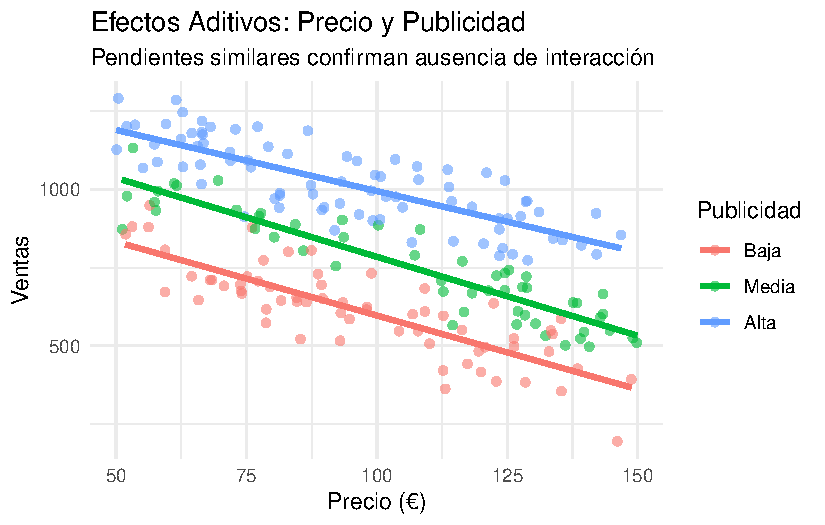
\includegraphics[keepaspectratio]{tema3_files/figure-pdf/visualizacion-interaccion-1.pdf}}

\textbf{Interpretación crítica: Visual vs Estadística}

Observando el gráfico, las líneas \textbf{parecen tener pendientes
diferentes}, lo que visualmente sugeriría la presencia de interacción.
Sin embargo, el análisis estadístico formal nos indica que esta
diferencia \textbf{no es estadísticamente significativa} (p = 0.435).

\textbf{¿Por qué esta aparente contradicción?}

\begin{itemize}
\tightlist
\item
  \textbf{Variabilidad aleatoria}: Las diferencias observadas pueden
  deberse al ruido aleatorio en los datos
\item
  \textbf{Tamaño de muestra}: Puede no ser suficiente para detectar una
  interacción débil si realmente existe
\item
  \textbf{Poder estadístico}: El test puede no tener suficiente poder
  para detectar efectos pequeños
\item
  \textbf{Agrupación artificial}: Los grupos de publicidad se crearon
  artificialmente para visualización, no reflejan la variable continua
  real
\end{itemize}

\textbf{Decisión metodológica correcta:}

\begin{itemize}
\tightlist
\item
  \textbf{Confiar en la estadística formal}: El p-valor \textgreater{}
  0.05 indica no significancia
\item
  \textbf{Modelo parsimonioso}: Eliminar el término de interacción no
  significativo
\item
  \textbf{Interpretación conservadora}: Los efectos son aditivos hasta
  que se demuestre lo contrario
\end{itemize}

\textbf{Lección crucial:}

Este ejemplo demuestra por qué \textbf{la inspección visual nunca debe
ser el único criterio} para decidir sobre la inclusión de términos de
interacción. La estadística inferencial formal debe prevalecer sobre las
impresiones visuales, especialmente cuando hay incertidumbre debido a la
variabilidad muestral.

\textbf{Modelo final recomendado:}
\texttt{ventas\ \textasciitilde{}\ precio\ +\ publicidad} (sin
interacción)

\end{tcolorbox}

\subsection{Interacciones entre variables
categóricas}\label{interacciones-entre-variables-categuxf3ricas}

Cuando ambas variables son categóricas, las interacciones representan
efectos específicos de combinaciones de categorías que no pueden
explicarse por los efectos principales por separado.

Para dos variables categóricas A (con niveles i) y B (con niveles j), el
modelo incluye:

\[Y = \mu + \alpha_i + \beta_j + (\alpha\beta)_{ij} + \varepsilon\]

Donde \((\alpha\beta)_{ij}\) representa la interacción específica entre
el nivel i de A y el nivel j de B.

La interacción \((\alpha\beta)_{ij}\) indica cuánto la combinación
específica (i,j) se desvía del efecto que esperaríamos si solo sumáramos
los efectos principales \(\alpha_i + \beta_j\).

\begin{tcolorbox}[enhanced jigsaw, leftrule=.75mm, breakable, colbacktitle=quarto-callout-tip-color!10!white, bottomrule=.15mm, colframe=quarto-callout-tip-color-frame, toprule=.15mm, colback=white, coltitle=black, bottomtitle=1mm, left=2mm, title=\textcolor{quarto-callout-tip-color}{\faLightbulb}\hspace{0.5em}{Ejemplo: Interacción género-departamento en salarios}, opacityback=0, arc=.35mm, opacitybacktitle=0.6, toptitle=1mm, titlerule=0mm, rightrule=.15mm]

\begin{Shaded}
\begin{Highlighting}[]
\CommentTok{\# Simulación: salarios por género y departamento con interacción}
\CommentTok{\# (brecha salarial varía según departamento)}
\FunctionTok{set.seed}\NormalTok{(}\DecValTok{456}\NormalTok{)}
\NormalTok{n }\OtherTok{\textless{}{-}} \DecValTok{300}

\CommentTok{\# Variables categóricas}
\NormalTok{genero }\OtherTok{\textless{}{-}} \FunctionTok{sample}\NormalTok{(}\FunctionTok{c}\NormalTok{(}\StringTok{"Masculino"}\NormalTok{, }\StringTok{"Femenino"}\NormalTok{), n, }\AttributeTok{replace =} \ConstantTok{TRUE}\NormalTok{)}
\NormalTok{departamento }\OtherTok{\textless{}{-}} \FunctionTok{sample}\NormalTok{(}\FunctionTok{c}\NormalTok{(}\StringTok{"Ventas"}\NormalTok{, }\StringTok{"IT"}\NormalTok{, }\StringTok{"RRHH"}\NormalTok{), n, }\AttributeTok{replace =} \ConstantTok{TRUE}\NormalTok{)}

\CommentTok{\# Efectos principales y de interacción simulados}
\NormalTok{efecto\_base }\OtherTok{\textless{}{-}} \DecValTok{40000}  \CommentTok{\# salario base}
\NormalTok{efecto\_masculino }\OtherTok{\textless{}{-}} \FunctionTok{ifelse}\NormalTok{(genero }\SpecialCharTok{==} \StringTok{"Masculino"}\NormalTok{, }\DecValTok{2000}\NormalTok{, }\DecValTok{0}\NormalTok{)}
\NormalTok{efecto\_it }\OtherTok{\textless{}{-}} \FunctionTok{ifelse}\NormalTok{(departamento }\SpecialCharTok{==} \StringTok{"IT"}\NormalTok{, }\DecValTok{8000}\NormalTok{, }\DecValTok{0}\NormalTok{)}
\NormalTok{efecto\_rrhh }\OtherTok{\textless{}{-}} \FunctionTok{ifelse}\NormalTok{(departamento }\SpecialCharTok{==} \StringTok{"RRHH"}\NormalTok{, }\DecValTok{3000}\NormalTok{, }\DecValTok{0}\NormalTok{)}

\CommentTok{\# Interacción: brecha de género mayor en IT}
\NormalTok{interaccion }\OtherTok{\textless{}{-}} \FunctionTok{ifelse}\NormalTok{(genero }\SpecialCharTok{==} \StringTok{"Masculino"} \SpecialCharTok{\&}\NormalTok{ departamento }\SpecialCharTok{==} \StringTok{"IT"}\NormalTok{, }\DecValTok{4000}\NormalTok{, }\DecValTok{0}\NormalTok{)}

\NormalTok{salario }\OtherTok{\textless{}{-}}\NormalTok{ efecto\_base }\SpecialCharTok{+}\NormalTok{ efecto\_masculino }\SpecialCharTok{+}\NormalTok{ efecto\_it }\SpecialCharTok{+}\NormalTok{ efecto\_rrhh }\SpecialCharTok{+} 
\NormalTok{           interaccion }\SpecialCharTok{+} \FunctionTok{rnorm}\NormalTok{(n, }\DecValTok{0}\NormalTok{, }\DecValTok{3000}\NormalTok{)}

\NormalTok{datos\_cat }\OtherTok{\textless{}{-}} \FunctionTok{data.frame}\NormalTok{(genero, departamento, salario)}

\CommentTok{\# Modelo con interacción}
\NormalTok{modelo\_cat }\OtherTok{\textless{}{-}} \FunctionTok{lm}\NormalTok{(salario }\SpecialCharTok{\textasciitilde{}}\NormalTok{ genero }\SpecialCharTok{*}\NormalTok{ departamento, }\AttributeTok{data =}\NormalTok{ datos\_cat)}
\FunctionTok{summary}\NormalTok{(modelo\_cat)}
\end{Highlighting}
\end{Shaded}

\begin{verbatim}

Call:
lm(formula = salario ~ genero * departamento, data = datos_cat)

Residuals:
    Min      1Q  Median      3Q     Max 
-8037.9 -1930.7    48.4  1968.1  7486.9 

Coefficients:
                                   Estimate Std. Error t value Pr(>|t|)    
(Intercept)                         47627.4      461.2 103.270  < 2e-16 ***
generoMasculino                      6166.3      593.4  10.391  < 2e-16 ***
departamentoRRHH                    -4433.3      633.9  -6.994 1.80e-11 ***
departamentoVentas                  -7744.7      597.4 -12.964  < 2e-16 ***
generoMasculino:departamentoRRHH    -4007.2      857.1  -4.675 4.48e-06 ***
generoMasculino:departamentoVentas  -3793.8      814.4  -4.659 4.83e-06 ***
---
Signif. codes:  0 '***' 0.001 '**' 0.01 '*' 0.05 '.' 0.1 ' ' 1

Residual standard error: 2917 on 294 degrees of freedom
Multiple R-squared:  0.7372,    Adjusted R-squared:  0.7327 
F-statistic: 164.9 on 5 and 294 DF,  p-value: < 2.2e-16
\end{verbatim}

\begin{Shaded}
\begin{Highlighting}[]
\CommentTok{\# Medias por grupo para interpretar la interacción}
\NormalTok{medias\_grupo }\OtherTok{\textless{}{-}} \FunctionTok{aggregate}\NormalTok{(salario }\SpecialCharTok{\textasciitilde{}}\NormalTok{ genero }\SpecialCharTok{+}\NormalTok{ departamento, }\AttributeTok{data =}\NormalTok{ datos\_cat, }\AttributeTok{FUN =}\NormalTok{ mean)}
\NormalTok{medias\_grupo }\OtherTok{\textless{}{-}}\NormalTok{ medias\_grupo[}\FunctionTok{order}\NormalTok{(medias\_grupo}\SpecialCharTok{$}\NormalTok{departamento, medias\_grupo}\SpecialCharTok{$}\NormalTok{genero), ]}
\FunctionTok{kable}\NormalTok{(medias\_grupo, }\AttributeTok{caption =} \StringTok{"Salario promedio por género y departamento"}\NormalTok{)}
\end{Highlighting}
\end{Shaded}

\begin{longtable}[]{@{}llr@{}}
\caption{Salario promedio por género y departamento}\tabularnewline
\toprule\noalign{}
genero & departamento & salario \\
\midrule\noalign{}
\endfirsthead
\toprule\noalign{}
genero & departamento & salario \\
\midrule\noalign{}
\endhead
\bottomrule\noalign{}
\endlastfoot
Femenino & IT & 47627.44 \\
Masculino & IT & 53793.71 \\
Femenino & RRHH & 43194.15 \\
Masculino & RRHH & 45353.23 \\
Femenino & Ventas & 39882.76 \\
Masculino & Ventas & 42255.23 \\
\end{longtable}

\begin{Shaded}
\begin{Highlighting}[]
\CommentTok{\# Visualización de la interacción}
\FunctionTok{library}\NormalTok{(ggplot2)}
\FunctionTok{ggplot}\NormalTok{(datos\_cat, }\FunctionTok{aes}\NormalTok{(}\AttributeTok{x =}\NormalTok{ departamento, }\AttributeTok{y =}\NormalTok{ salario, }\AttributeTok{fill =}\NormalTok{ genero)) }\SpecialCharTok{+}
  \FunctionTok{geom\_boxplot}\NormalTok{(}\AttributeTok{position =} \StringTok{"dodge"}\NormalTok{) }\SpecialCharTok{+}
  \FunctionTok{stat\_summary}\NormalTok{(}\AttributeTok{fun =}\NormalTok{ mean, }\AttributeTok{geom =} \StringTok{"point"}\NormalTok{, }\AttributeTok{shape =} \DecValTok{23}\NormalTok{, }\AttributeTok{size =} \DecValTok{3}\NormalTok{, }
               \AttributeTok{position =} \FunctionTok{position\_dodge}\NormalTok{(}\FloatTok{0.75}\NormalTok{)) }\SpecialCharTok{+}
  \FunctionTok{labs}\NormalTok{(}\AttributeTok{title =} \StringTok{"Interacción Género{-}Departamento en Salarios"}\NormalTok{,}
       \AttributeTok{x =} \StringTok{"Departamento"}\NormalTok{, }\AttributeTok{y =} \StringTok{"Salario (€)"}\NormalTok{, }\AttributeTok{fill =} \StringTok{"Género"}\NormalTok{) }\SpecialCharTok{+}
  \FunctionTok{theme\_minimal}\NormalTok{()}
\end{Highlighting}
\end{Shaded}

\pandocbounded{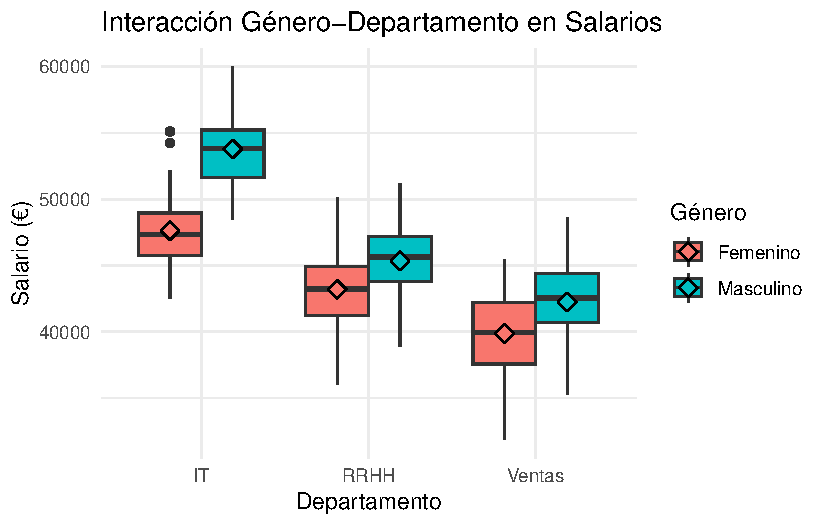
\includegraphics[keepaspectratio]{tema3_files/figure-pdf/interaccion-categorica-categorica-1.pdf}}

\textbf{Evidencia visual clara:} El segundo gráfico (boxplots por género
y departamento) revela \textbf{patrones de interacción marcados} que se
manifiestan de forma diferente en cada departamento.

\textbf{Patrones específicos por departamento:}

\begin{itemize}
\tightlist
\item
  \textbf{IT:} La brecha de género es \textbf{máxima}
  (\textasciitilde€8,000). Los hombres tienen salarios
  significativamente superiores y mayor variabilidad salarial
\item
  \textbf{RRHH:} Brecha \textbf{moderada} (\textasciitilde€3,000) con
  distribuciones más similares entre géneros
\item
  \textbf{Ventas:} \textbf{Menor brecha de género}
  (\textasciitilde€1,500), con salarios más homogéneos entre grupos
\end{itemize}

\textbf{Interpretación de la interacción:} Las \textbf{líneas no
paralelas} en el patrón de medias confirman que el efecto del género
sobre el salario \textbf{varía significativamente según el
departamento}. Esto sugiere:

\begin{itemize}
\tightlist
\item
  Diferencias en \textbf{culturas departamentales} respecto a equidad
  salarial
\item
  \textbf{Estructuras de compensación} variables entre departamentos
\item
  Posibles diferencias en \textbf{poder de negociación} o
  \textbf{demanda de talento}
\end{itemize}

\textbf{Implicaciones organizacionales:} La interacción indica que las
políticas salariales no son uniformes y que intervenciones de equidad
deberían ser \textbf{diferenciadas por departamento}.

\textbf{Gráfico de interacción clásico:}

\begin{Shaded}
\begin{Highlighting}[]
\CommentTok{\# Calcular medias y errores estándar por grupo para el gráfico}
\FunctionTok{suppressPackageStartupMessages}\NormalTok{(}\FunctionTok{library}\NormalTok{(dplyr))}
\NormalTok{medias\_se }\OtherTok{\textless{}{-}}\NormalTok{ datos\_cat }\SpecialCharTok{\%\textgreater{}\%}
  \FunctionTok{group\_by}\NormalTok{(genero, departamento) }\SpecialCharTok{\%\textgreater{}\%}
  \FunctionTok{summarise}\NormalTok{(}
    \AttributeTok{media =} \FunctionTok{mean}\NormalTok{(salario),}
    \AttributeTok{se =} \FunctionTok{sd}\NormalTok{(salario) }\SpecialCharTok{/} \FunctionTok{sqrt}\NormalTok{(}\FunctionTok{n}\NormalTok{()),}
    \AttributeTok{.groups =} \StringTok{"drop"}
\NormalTok{  )}

\CommentTok{\# Mostrar los datos calculados}
\FunctionTok{kable}\NormalTok{(medias\_se, }\AttributeTok{caption =} \StringTok{"Medias y errores estándar por grupo"}\NormalTok{)}
\end{Highlighting}
\end{Shaded}

\begin{longtable}[]{@{}llrr@{}}
\caption{Medias y errores estándar por grupo}\tabularnewline
\toprule\noalign{}
genero & departamento & media & se \\
\midrule\noalign{}
\endfirsthead
\toprule\noalign{}
genero & departamento & media & se \\
\midrule\noalign{}
\endhead
\bottomrule\noalign{}
\endlastfoot
Femenino & IT & 47627.44 & 463.4703 \\
Femenino & RRHH & 43194.15 & 443.9292 \\
Femenino & Ventas & 39882.76 & 378.5932 \\
Masculino & IT & 53793.71 & 371.1923 \\
Masculino & RRHH & 45353.23 & 425.9146 \\
Masculino & Ventas & 42255.23 & 414.4745 \\
\end{longtable}

\begin{Shaded}
\begin{Highlighting}[]
\CommentTok{\# Gráfico de interacción estilo clásico}
\FunctionTok{ggplot}\NormalTok{(medias\_se, }\FunctionTok{aes}\NormalTok{(}\AttributeTok{x =}\NormalTok{ departamento, }\AttributeTok{y =}\NormalTok{ media, }\AttributeTok{color =}\NormalTok{ genero, }\AttributeTok{group =}\NormalTok{ genero)) }\SpecialCharTok{+}
  \FunctionTok{geom\_point}\NormalTok{(}\AttributeTok{size =} \DecValTok{3}\NormalTok{) }\SpecialCharTok{+}
  \FunctionTok{geom\_line}\NormalTok{(}\AttributeTok{linewidth =} \DecValTok{1}\NormalTok{) }\SpecialCharTok{+}
  \FunctionTok{geom\_errorbar}\NormalTok{(}\FunctionTok{aes}\NormalTok{(}\AttributeTok{ymin =}\NormalTok{ media }\SpecialCharTok{{-}}\NormalTok{ se, }\AttributeTok{ymax =}\NormalTok{ media }\SpecialCharTok{+}\NormalTok{ se), }\AttributeTok{width =} \FloatTok{0.1}\NormalTok{) }\SpecialCharTok{+}
  \FunctionTok{labs}\NormalTok{(}\AttributeTok{title =} \StringTok{"Gráfico de Interacción: Género × Departamento"}\NormalTok{,}
       \AttributeTok{subtitle =} \StringTok{"Las líneas no paralelas indican presencia de interacción"}\NormalTok{,}
       \AttributeTok{x =} \StringTok{"Departamento"}\NormalTok{, }\AttributeTok{y =} \StringTok{"Salario promedio (€)"}\NormalTok{, }\AttributeTok{color =} \StringTok{"Género"}\NormalTok{) }\SpecialCharTok{+}
  \FunctionTok{theme\_minimal}\NormalTok{() }\SpecialCharTok{+}
  \FunctionTok{theme}\NormalTok{(}\AttributeTok{plot.subtitle =} \FunctionTok{element\_text}\NormalTok{(}\AttributeTok{size =} \DecValTok{10}\NormalTok{, }\AttributeTok{color =} \StringTok{"gray50"}\NormalTok{))}
\end{Highlighting}
\end{Shaded}

\pandocbounded{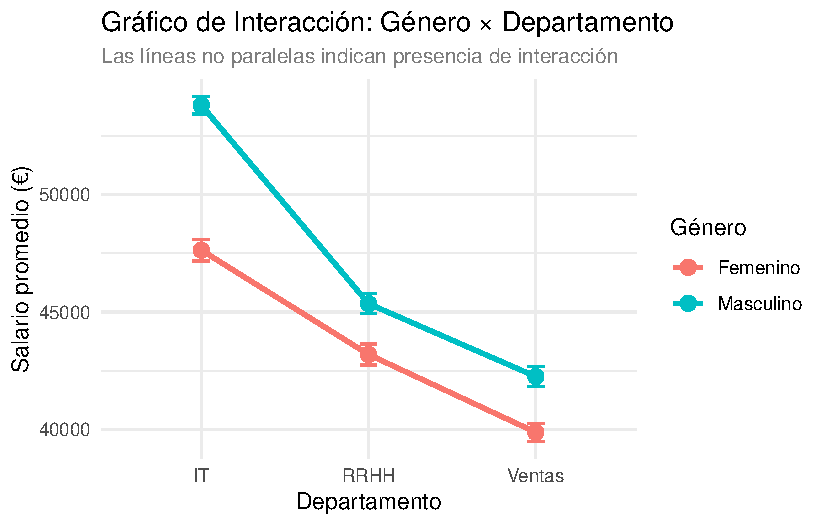
\includegraphics[keepaspectratio]{tema3_files/figure-pdf/grafico-interaccion-viz-1.pdf}}

\textbf{Interpretación del gráfico:} Las líneas \textbf{no son
paralelas}, confirmando la presencia de interacción significativa. La
brecha salarial de género varía considerablemente: mayor en IT, moderada
en RRHH, y menor en Ventas.

\end{tcolorbox}

\subsection{Interacciones mixtas (continua ×
categórica)}\label{interacciones-mixtas-continua-categuxf3rica}

Las interacciones mixtas son especialmente útiles para modelar cómo el
efecto de una variable continua varía entre grupos categóricos. Esto es
fundamental cuando sospechamos que la relación funcional cambia según el
contexto definido por la variable categórica.

\textbf{Formulación matemática:}
\[Y = \beta_0 + \beta_1 X + \beta_2 D + \beta_3 X \cdot D + \varepsilon\]

Donde D es una variable dummy (0/1) que representa la variable
categórica.

\textbf{Interpretación geométrica:} La interacción permite que cada
grupo categórico tenga:

\begin{itemize}
\tightlist
\item
  \textbf{Intercepto diferente}: \(\beta_0\) (grupo de referencia)
  vs.~\(\beta_0 + \beta_2\) (otro grupo)\\
\item
  \textbf{Pendiente diferente}: \(\beta_1\) (grupo de referencia)
  vs.~\(\beta_1 + \beta_3\) (otro grupo)
\end{itemize}

\begin{tcolorbox}[enhanced jigsaw, leftrule=.75mm, breakable, colbacktitle=quarto-callout-tip-color!10!white, bottomrule=.15mm, colframe=quarto-callout-tip-color-frame, toprule=.15mm, colback=white, coltitle=black, bottomtitle=1mm, left=2mm, title=\textcolor{quarto-callout-tip-color}{\faLightbulb}\hspace{0.5em}{Ejemplo: Interacción experiencia-género en salarios}, opacityback=0, arc=.35mm, opacitybacktitle=0.6, toptitle=1mm, titlerule=0mm, rightrule=.15mm]

\begin{Shaded}
\begin{Highlighting}[]
\CommentTok{\# Simulación: efecto de experiencia en salario varía según género}
\FunctionTok{set.seed}\NormalTok{(}\DecValTok{789}\NormalTok{)}
\NormalTok{n }\OtherTok{\textless{}{-}} \DecValTok{250}

\NormalTok{experiencia }\OtherTok{\textless{}{-}} \FunctionTok{runif}\NormalTok{(n, }\DecValTok{0}\NormalTok{, }\DecValTok{20}\NormalTok{)  }\CommentTok{\# años de experiencia}
\NormalTok{genero }\OtherTok{\textless{}{-}} \FunctionTok{sample}\NormalTok{(}\FunctionTok{c}\NormalTok{(}\StringTok{"Femenino"}\NormalTok{, }\StringTok{"Masculino"}\NormalTok{), n, }\AttributeTok{replace =} \ConstantTok{TRUE}\NormalTok{)}

\CommentTok{\# Efecto diferencial: pendiente de experiencia menor para mujeres}
\NormalTok{salario\_base }\OtherTok{\textless{}{-}} \DecValTok{35000}
\NormalTok{efecto\_experiencia\_hombres }\OtherTok{\textless{}{-}} \DecValTok{2000}  \CommentTok{\# €2000 por año para hombres}
\NormalTok{efecto\_experiencia\_mujeres }\OtherTok{\textless{}{-}} \DecValTok{1200}  \CommentTok{\# €1200 por año para mujeres (brecha creciente)}
\NormalTok{efecto\_genero\_base }\OtherTok{\textless{}{-}} \FunctionTok{ifelse}\NormalTok{(genero }\SpecialCharTok{==} \StringTok{"Masculino"}\NormalTok{, }\DecValTok{3000}\NormalTok{, }\DecValTok{0}\NormalTok{)}

\CommentTok{\# Crear variable dummy para interacción}
\NormalTok{dummy\_masculino }\OtherTok{\textless{}{-}} \FunctionTok{ifelse}\NormalTok{(genero }\SpecialCharTok{==} \StringTok{"Masculino"}\NormalTok{, }\DecValTok{1}\NormalTok{, }\DecValTok{0}\NormalTok{)}

\CommentTok{\# Salario con interacción}
\NormalTok{salario }\OtherTok{\textless{}{-}}\NormalTok{ salario\_base }\SpecialCharTok{+} 
\NormalTok{           efecto\_experiencia\_mujeres }\SpecialCharTok{*}\NormalTok{ experiencia }\SpecialCharTok{+}  \CommentTok{\# pendiente base (mujeres)}
\NormalTok{           efecto\_genero\_base }\SpecialCharTok{*}\NormalTok{ dummy\_masculino }\SpecialCharTok{+}      \CommentTok{\# diferencia intercepto}
\NormalTok{           (efecto\_experiencia\_hombres }\SpecialCharTok{{-}}\NormalTok{ efecto\_experiencia\_mujeres) }\SpecialCharTok{*}\NormalTok{ experiencia }\SpecialCharTok{*}\NormalTok{ dummy\_masculino }\SpecialCharTok{+}  \CommentTok{\# interacción}
           \FunctionTok{rnorm}\NormalTok{(n, }\DecValTok{0}\NormalTok{, }\DecValTok{4000}\NormalTok{)}

\NormalTok{datos\_mixta }\OtherTok{\textless{}{-}} \FunctionTok{data.frame}\NormalTok{(experiencia, genero, salario, dummy\_masculino)}

\CommentTok{\# Modelo con interacción}
\NormalTok{modelo\_mixta }\OtherTok{\textless{}{-}} \FunctionTok{lm}\NormalTok{(salario }\SpecialCharTok{\textasciitilde{}}\NormalTok{ experiencia }\SpecialCharTok{*}\NormalTok{ genero, }\AttributeTok{data =}\NormalTok{ datos\_mixta)}
\FunctionTok{summary}\NormalTok{(modelo\_mixta)}
\end{Highlighting}
\end{Shaded}

\begin{verbatim}

Call:
lm(formula = salario ~ experiencia * genero, data = datos_mixta)

Residuals:
     Min       1Q   Median       3Q      Max 
-12340.2  -2742.7    162.8   2586.6   9293.8 

Coefficients:
                            Estimate Std. Error t value Pr(>|t|)    
(Intercept)                 35650.27     765.04  46.599   <2e-16 ***
experiencia                  1123.03      69.74  16.103   <2e-16 ***
generoMasculino              2613.33    1038.08   2.517   0.0125 *  
experiencia:generoMasculino   905.46      92.44   9.795   <2e-16 ***
---
Signif. codes:  0 '***' 0.001 '**' 0.01 '*' 0.05 '.' 0.1 ' ' 1

Residual standard error: 3995 on 246 degrees of freedom
Multiple R-squared:  0.8889,    Adjusted R-squared:  0.8876 
F-statistic: 656.2 on 3 and 246 DF,  p-value: < 2.2e-16
\end{verbatim}

\textbf{Interpretación detallada de los coeficientes:}

\begin{Shaded}
\begin{Highlighting}[]
\CommentTok{\# Extraer coeficientes para interpretación}
\NormalTok{coef\_mixta }\OtherTok{\textless{}{-}} \FunctionTok{coef}\NormalTok{(modelo\_mixta)}

\CommentTok{\# Crear tabla de interpretación por género}
\NormalTok{tabla\_genero }\OtherTok{\textless{}{-}} \FunctionTok{data.frame}\NormalTok{(}
\NormalTok{  Parámetro }\OtherTok{=} \FunctionTok{c}\NormalTok{(}\StringTok{"Intercepto (salario inicial)"}\NormalTok{, }\StringTok{"Pendiente (€ por año experiencia)"}\NormalTok{),}
  \AttributeTok{Mujeres =} \FunctionTok{c}\NormalTok{(}
    \FunctionTok{paste0}\NormalTok{(}\StringTok{"€"}\NormalTok{, }\FunctionTok{format}\NormalTok{(}\FunctionTok{round}\NormalTok{(coef\_mixta[}\DecValTok{1}\NormalTok{], }\DecValTok{0}\NormalTok{), }\AttributeTok{big.mark =} \StringTok{","}\NormalTok{)),}
    \FunctionTok{paste0}\NormalTok{(}\StringTok{"€"}\NormalTok{, }\FunctionTok{round}\NormalTok{(coef\_mixta[}\DecValTok{2}\NormalTok{], }\DecValTok{0}\NormalTok{))}
\NormalTok{  ),}
  \AttributeTok{Hombres =} \FunctionTok{c}\NormalTok{(}
    \FunctionTok{paste0}\NormalTok{(}\StringTok{"€"}\NormalTok{, }\FunctionTok{format}\NormalTok{(}\FunctionTok{round}\NormalTok{(coef\_mixta[}\DecValTok{1}\NormalTok{] }\SpecialCharTok{+}\NormalTok{ coef\_mixta[}\DecValTok{3}\NormalTok{], }\DecValTok{0}\NormalTok{), }\AttributeTok{big.mark =} \StringTok{","}\NormalTok{)),}
    \FunctionTok{paste0}\NormalTok{(}\StringTok{"€"}\NormalTok{, }\FunctionTok{round}\NormalTok{(coef\_mixta[}\DecValTok{2}\NormalTok{] }\SpecialCharTok{+}\NormalTok{ coef\_mixta[}\DecValTok{4}\NormalTok{], }\DecValTok{0}\NormalTok{))}
\NormalTok{  ),}
  \AttributeTok{Diferencia =} \FunctionTok{c}\NormalTok{(}
    \FunctionTok{paste0}\NormalTok{(}\StringTok{"€"}\NormalTok{, }\FunctionTok{format}\NormalTok{(}\FunctionTok{round}\NormalTok{(coef\_mixta[}\DecValTok{3}\NormalTok{], }\DecValTok{0}\NormalTok{), }\AttributeTok{big.mark =} \StringTok{","}\NormalTok{)),}
    \FunctionTok{paste0}\NormalTok{(}\StringTok{"€"}\NormalTok{, }\FunctionTok{round}\NormalTok{(coef\_mixta[}\DecValTok{4}\NormalTok{], }\DecValTok{0}\NormalTok{), }\StringTok{" adicionales"}\NormalTok{)}
\NormalTok{  )}
\NormalTok{)}

\FunctionTok{kable}\NormalTok{(tabla\_genero, }
      \AttributeTok{caption =} \StringTok{"Comparación de parámetros del modelo por género"}\NormalTok{)}
\end{Highlighting}
\end{Shaded}

\begin{longtable}[]{@{}llll@{}}
\caption{Comparación de parámetros del modelo por género}\tabularnewline
\toprule\noalign{}
Parámetro & Mujeres & Hombres & Diferencia \\
\midrule\noalign{}
\endfirsthead
\toprule\noalign{}
Parámetro & Mujeres & Hombres & Diferencia \\
\midrule\noalign{}
\endhead
\bottomrule\noalign{}
\endlastfoot
Intercepto (salario inicial) & €35,650 & €38,264 & €2,613 \\
Pendiente (€ por año experiencia) & €1123 & €2028 & €905 adicionales \\
\end{longtable}

\textbf{Implicaciones de la interacción:}

El coeficiente de interacción (\textbf{905}) indica que cada año
adicional de experiencia aumenta el salario masculino en \textbf{€905
más} que el salario femenino. Esto crea una \textbf{brecha creciente}:
inicialmente la diferencia es de €2,613, pero después de 20 años de
experiencia, la brecha total alcanza €20,722.

\textbf{Visualización de la divergencia salarial:}

\begin{Shaded}
\begin{Highlighting}[]
\CommentTok{\# Visualización de líneas de regresión por grupo}
\FunctionTok{ggplot}\NormalTok{(datos\_mixta, }\FunctionTok{aes}\NormalTok{(}\AttributeTok{x =}\NormalTok{ experiencia, }\AttributeTok{y =}\NormalTok{ salario, }\AttributeTok{color =}\NormalTok{ genero)) }\SpecialCharTok{+}
  \FunctionTok{geom\_point}\NormalTok{(}\AttributeTok{alpha =} \FloatTok{0.6}\NormalTok{) }\SpecialCharTok{+}
  \FunctionTok{geom\_smooth}\NormalTok{(}\AttributeTok{method =} \StringTok{"lm"}\NormalTok{, }\AttributeTok{formula =}\NormalTok{ y }\SpecialCharTok{\textasciitilde{}}\NormalTok{ x, }\AttributeTok{se =} \ConstantTok{TRUE}\NormalTok{, }\AttributeTok{linewidth =} \FloatTok{1.2}\NormalTok{) }\SpecialCharTok{+}
  \FunctionTok{labs}\NormalTok{(}\AttributeTok{title =} \StringTok{"Interacción Experiencia{-}Género: Brechas Crecientes"}\NormalTok{,}
       \AttributeTok{subtitle =} \StringTok{"La brecha salarial se amplía con la experiencia"}\NormalTok{,}
       \AttributeTok{x =} \StringTok{"Años de experiencia"}\NormalTok{, }\AttributeTok{y =} \StringTok{"Salario (€)"}\NormalTok{, }\AttributeTok{color =} \StringTok{"Género"}\NormalTok{) }\SpecialCharTok{+}
  \FunctionTok{theme\_minimal}\NormalTok{() }\SpecialCharTok{+}
  \FunctionTok{scale\_color\_manual}\NormalTok{(}\AttributeTok{values =} \FunctionTok{c}\NormalTok{(}\StringTok{"Femenino"} \OtherTok{=} \StringTok{"\#E69F00"}\NormalTok{, }\StringTok{"Masculino"} \OtherTok{=} \StringTok{"\#0072B2"}\NormalTok{)) }\SpecialCharTok{+}
  \FunctionTok{scale\_y\_continuous}\NormalTok{(}\AttributeTok{labels =}\NormalTok{ scales}\SpecialCharTok{::}\FunctionTok{comma\_format}\NormalTok{(}\AttributeTok{suffix =} \StringTok{"€"}\NormalTok{))}
\end{Highlighting}
\end{Shaded}

\pandocbounded{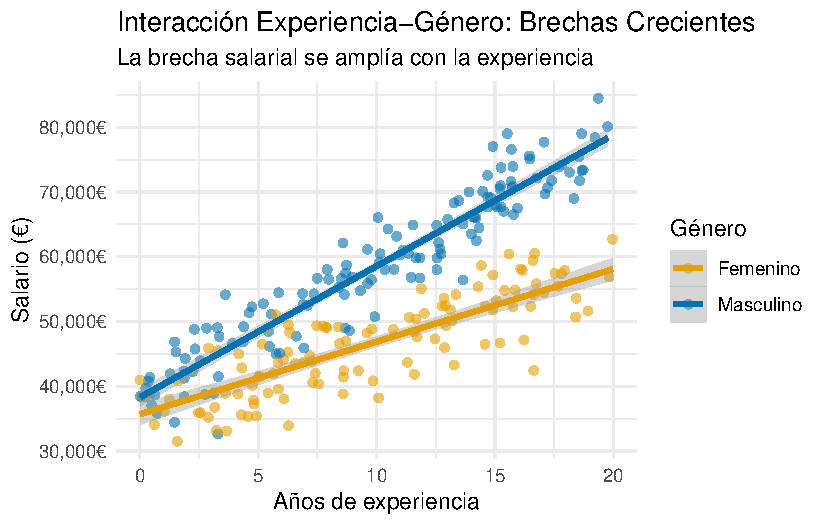
\includegraphics[keepaspectratio]{tema3_files/figure-pdf/visualizacion-mixta-1.pdf}}

\textbf{Evidencia de brechas crecientes:} El tercer gráfico (scatter
plot con líneas de regresión) demuestra claramente el patrón de
\textbf{interacción experiencia-género} mediante \textbf{líneas
divergentes} con pendientes notablemente diferentes.

\textbf{Interpretación cuantitativa de la divergencia:}

\begin{itemize}
\tightlist
\item
  \textbf{Punto de inicio (0 años):} Brecha inicial de €2,613 a favor de
  los hombres
\item
  \textbf{Pendientes diferenciadas:} Los hombres ganan €2028 adicionales
  por año vs.~€1123 para las mujeres
\item
  \textbf{Brecha acumulativa:} Cada año adicional de experiencia
  \textbf{amplía la brecha} en €905 adicionales
\end{itemize}

\textbf{Implicaciones del patrón de interacción:} La \textbf{divergencia
progresiva} visible en las líneas revela que:

\begin{itemize}
\tightlist
\item
  El \textbf{retorno a la experiencia} es sistemáticamente \textbf{mayor
  para hombres} que para mujeres
\item
  A los 20 años de experiencia, la brecha total alcanza €20,722 (inicial
  + acumulativa)
\item
  Este patrón sugiere \textbf{barreras estructurales} que impiden que
  las mujeres capitalicen plenamente su experiencia
\end{itemize}

\textbf{Significancia social:} Esta interacción documenta un fenómeno
preocupante donde la \textbf{inequidad salarial se agrava con el
tiempo}, indicando que las brechas de género no son meramente
diferencias de entrada sino \textbf{desventajas acumulativas} a lo largo
de la carrera profesional.

\end{tcolorbox}

\subsection{Identificación y detección de
interacciones}\label{identificaciuxf3n-y-detecciuxf3n-de-interacciones}

La detección sistemática de interacciones requiere combinar
justificación teórica, exploración visual y validación estadística. No
debemos buscar interacciones aleatoriamente, sino guiados por el
conocimiento del dominio y patrones observables en los datos.

La justificación teórica previa es fundamental: la teoría del dominio
debe sugerir dónde pueden existir interacciones. Por ejemplo, en
economía esperamos efectos precio-publicidad o educación-experiencia; en
medicina son comunes las interacciones dosis-edad o
tratamiento-comorbilidad; en marketing encontramos interacciones
producto-canal o temporada-promoción.

La exploración visual sistemática complementa la teoría con evidencia
empírica. Para variables continuas utilizamos gráficos de dispersión
coloreados por grupos categóricos; para variables categóricas empleamos
gráficos de interacción (interaction plots); para interacciones mixtas
analizamos líneas de regresión por grupo.

Los tests estadísticos formales proporcionan validación objetiva: el
test F para interacciones compara modelos con y sin términos de
interacción, el test de significancia individual evalúa coeficientes
específicos mediante t-test, y los criterios de información (AIC/BIC)
guían la selección entre modelos alternativos.

\begin{tcolorbox}[enhanced jigsaw, leftrule=.75mm, breakable, colbacktitle=quarto-callout-note-color!10!white, bottomrule=.15mm, colframe=quarto-callout-note-color-frame, toprule=.15mm, colback=white, coltitle=black, bottomtitle=1mm, left=2mm, title=\textcolor{quarto-callout-note-color}{\faInfo}\hspace{0.5em}{Estrategia de modelado jerárquico}, opacityback=0, arc=.35mm, opacitybacktitle=0.6, toptitle=1mm, titlerule=0mm, rightrule=.15mm]

\textbf{Principio de jerarquía:} Si incluimos una interacción A×B,
siempre debemos incluir los efectos principales A y B, incluso si no son
significativos individualmente. Esto preserva la interpretabilidad y
evita sesgos en los coeficientes de interacción.

\textbf{Proceso de construcción del modelo:}

\begin{enumerate}
\def\labelenumi{\arabic{enumi}.}
\tightlist
\item
  \textbf{Modelo base}: Solo efectos principales
\item
  \textbf{Modelo con interacciones}: Agregar términos de interacción
  teoricamente justificados
\item
  \textbf{Comparación}: Test F para evaluar mejora significativa
\item
  \textbf{Selección}: Usar criterios estadísticos y de parsimonia
\item
  \textbf{Validación}: Verificar supuestos y estabilidad en datos de
  prueba
\end{enumerate}

\end{tcolorbox}

\subsection{Consideraciones prácticas y
limitaciones}\label{consideraciones-pruxe1cticas-y-limitaciones}

Las interacciones incrementan exponencialmente la complejidad
interpretativa del modelo. Un modelo con k efectos principales puede
tener hasta \(k(k-1)/2\) interacciones de segundo orden, y el número
crece exponencialmente con interacciones de orden superior. Esta
explosión combinatorial hace que incluso modelos aparentemente simples
se vuelvan rápidamente inmanejables desde el punto de vista
interpretativo. Como reglas prácticas para la complejidad, recomendamos
limitar a máximo 2-3 interacciones de segundo orden en modelos
explicativos, evitar interacciones de tercer orden salvo justificación
teórica muy sólida, y priorizar interacciones con efectos grandes sobre
mera significancia estadística.

\begin{tcolorbox}[enhanced jigsaw, leftrule=.75mm, breakable, colbacktitle=quarto-callout-warning-color!10!white, bottomrule=.15mm, colframe=quarto-callout-warning-color-frame, toprule=.15mm, colback=white, coltitle=black, bottomtitle=1mm, left=2mm, title=\textcolor{quarto-callout-warning-color}{\faExclamationTriangle}\hspace{0.5em}{Advertencia sobre interpretación}, opacityback=0, arc=.35mm, opacitybacktitle=0.6, toptitle=1mm, titlerule=0mm, rightrule=.15mm]

\textbf{Cuidado con la interpretación automática.} Las interacciones en
escalas transformadas tienen significados diferentes que en escalas
originales. Siempre verificar la interpretación en el contexto de la
transformación aplicada y considerar la retransformación para
comunicación con audiencias no técnicas.

\end{tcolorbox}

Un problema adicional surge cuando las interacciones crean
multicolinealidad severa, especialmente cuando las variables principales
están correlacionadas, se incluyen múltiples interacciones con variables
comunes, o se usan variables categóricas con muchos niveles. Esta
multicolinealidad puede hacer que los coeficientes individuales sean
inestables y difíciles de interpretar, incluso cuando el modelo en
conjunto funcione bien predictivamente. Las estrategias de mitigación
incluyen el centrado de variables continuas para reducir la correlación
entre X y X×Z, la selección cuidadosa de interacciones sin incluir todas
las combinaciones posibles, y el uso de métodos de regularización como
Ridge o Lasso cuando hay múltiples interacciones.

La situación se complica aún más cuando las variables están
transformadas (logarítmica, Box-Cox). En estos casos, la interpretación
de las interacciones adquiere significados completamente diferentes que
en escalas originales. Por ejemplo, en un modelo como
\(\log(Y) = \beta_0 + \beta_1 \log(X_1) + \beta_2 X_2 + \beta_3 \log(X_1) \cdot X_2 + \varepsilon\),
el coeficiente \(\beta_3\) representa cómo cambia la elasticidad de Y
respecto a X₁ cuando X₂ aumenta en una unidad, lo que requiere una
interpretación mucho más sofisticada que una interacción en escalas
lineales.

\begin{tcolorbox}[enhanced jigsaw, leftrule=.75mm, breakable, colbacktitle=quarto-callout-important-color!10!white, bottomrule=.15mm, colframe=quarto-callout-important-color-frame, toprule=.15mm, colback=white, coltitle=black, bottomtitle=1mm, left=2mm, title=\textcolor{quarto-callout-important-color}{\faExclamation}\hspace{0.5em}{Principios para el uso de interacciones}, opacityback=0, arc=.35mm, opacitybacktitle=0.6, toptitle=1mm, titlerule=0mm, rightrule=.15mm]

\begin{enumerate}
\def\labelenumi{\arabic{enumi}.}
\tightlist
\item
  \textbf{Justificación teórica primero}: No buscar interacciones sin
  base conceptual
\item
  \textbf{Principio de jerarquía}: Mantener efectos principales cuando
  se incluyen interacciones
\item
  \textbf{Parsimonia}: Preferir modelos simples que expliquen bien sobre
  modelos complejos
\item
  \textbf{Validación robusta}: Verificar estabilidad en múltiples
  contextos
\item
  \textbf{Interpretación cuidadosa}: Asegurar comprensión completa antes
  de conclusiones
\item
  \textbf{Comunicación efectiva}: Usar visualizaciones para explicar
  efectos complejos
\end{enumerate}

\end{tcolorbox}

Las interacciones son herramientas poderosas que pueden revelar patrones
importantes ocultos en los efectos principales. Sin embargo, su uso
requiere disciplina metodológica, justificación teórica sólida, y
validación rigurosa para evitar conclusiones espurias y modelos
sobreajustados.

\section{Ingeniería de características avanzada: combinaciones, ratios y
transformaciones}\label{ingenieruxeda-de-caracteruxedsticas-avanzada-combinaciones-ratios-y-transformaciones}

Más allá de las transformaciones individuales e interacciones, la
ingeniería de características avanzada implica crear nuevas variables
predictivas mediante combinaciones matemáticas, ratios y
transformaciones compuestas que capturen relaciones complejas no
evidentes en las variables originales (Kuhn and Johnson 2019). Esta
aproximación es fundamental cuando las variables individuales contienen
información parcial que, al combinarse, revelan patrones predictivos más
potentes.

\subsection{Combinaciones lineales y no
lineales}\label{combinaciones-lineales-y-no-lineales}

Las combinaciones lineales crean nuevas variables mediante sumas
ponderadas de variables existentes, útiles especialmente cuando
trabajamos con variables que miden aspectos relacionados del mismo
fenómeno pero con diferentes escalas o unidades.

\textbf{Ejemplos de combinaciones lineales efectivas:}

\begin{itemize}
\item
  \textbf{Índices compuestos}: Combinan múltiples indicadores en un
  score único que captura un constructo multidimensional. Por ejemplo,
  un índice de riesgo cardiovascular podría definirse como
  \texttt{índice\_salud\ =\ 0.4×presión\_arterial\_normalizada\ +\ 0.3×colesterol\_normalizada\ +\ 0.3×IMC\_normalizado}.
  Los pesos (0.4, 0.3, 0.3) reflejan la importancia relativa establecida
  por evidencia médica, creando una métrica integrada que es más
  informativa que cualquier indicador individual. Este tipo de índices
  son especialmente valiosos en dominios donde múltiples factores
  contribuyen conjuntamente al outcome de interés.
\item
  \textbf{Scores balanceados}: Representan equilibrios o trade-offs
  entre dimensiones competitivas. Un ejemplo típico es
  \texttt{balance\_trabajo\_vida\ =\ horas\_trabajo\ /\ (tiempo\_personal\ +\ tiempo\_familia\ +\ tiempo\_descanso)}.
  Esta métrica captura no solo la intensidad laboral, sino también su
  contexto relativo dentro del estilo de vida completo. Valores altos
  indican desbalance hacia el trabajo, mientras que valores cercanos a
  1.0 sugieren equilibrio saludable. Los scores balanceados son
  fundamentales para capturar dinámicas de compensación que no son
  evidentes en variables absolutas.
\item
  \textbf{Factores sintéticos}: Cuando múltiples variables
  correlacionadas miden aspectos del mismo constructo subyacente, pueden
  condensarse en un factor común que preserve la información esencial
  eliminando redundancia. Por ejemplo, si tenemos variables
  \texttt{ingresos}, \texttt{educación}, y
  \texttt{prestigio\_ocupacional} (todas correlacionadas), podemos crear
  un factor \texttt{estatus\_socioeconomico} que capture la varianza
  común. Esto es especialmente útil cuando la colinealidad entre
  predictores compromete la estabilidad del modelo, pero cada variable
  aporta información valiosa.
\end{itemize}

Las combinaciones no lineales van más allá de las sumas ponderadas para
capturar interacciones multiplicativas, sinergias y compensaciones entre
variables mediante productos, cocientes, potencias y funciones más
complejas:

\begin{itemize}
\item
  \textbf{Productos de eficiencia}: Capturan sinergias multiplicativas
  donde el rendimiento depende de la combinación simultánea de múltiples
  factores. Por ejemplo,
  \texttt{rendimiento\_efectivo\ =\ capacidad\_instalada\ ×\ utilización\_porcentual\ ×\ factor\_calidad}.
  Esta métrica reconoce que el rendimiento real no es aditivo: tener
  alta capacidad pero baja utilización, o alta utilización con problemas
  de calidad, resulta en rendimiento subóptimo. Los productos de
  eficiencia son esenciales en contextos operacionales donde el
  desempeño emerge de la coordinación entre recursos.
\item
  \textbf{Ratios de rendimiento ajustado por riesgo}: Normalizan
  beneficios por su costo o riesgo asociado, creando métricas
  comparables entre contextos diferentes. Un ejemplo financiero sería
  \texttt{eficiencia\_ajustada\ =\ (rendimiento\_esperado\ -\ tasa\_libre\_riesgo)\ /\ (volatilidad\ +\ costos\_transaccion)}.
  Esta formulación reconoce que los rendimientos absolutos son engañosos
  sin considerar el riesgo asumido y los costos incurridos. Los ratios
  ajustados son cruciales para decisiones de optimización donde debemos
  comparar alternativas con perfiles de riesgo-retorno heterogéneos.
\item
  \textbf{Funciones de utilidad}: Capturan percepciones subjetivas o
  valores no lineales mediante transformaciones que reflejan
  preferencias reales. Por ejemplo,
  \texttt{valor\_percibido\ =\ √(calidad\_producto)\ ×\ precio⁻⁰·⁵}
  reconoce que la utilidad del consumidor tiene rendimientos
  decrecientes tanto en calidad como en ahorro de precio. La raíz
  cuadrada de la calidad refleja que mejoras incrementales tienen menor
  impacto en niveles altos, mientras que el exponente negativo del
  precio captura la sensibilidad decreciente a cambios de precio en
  productos caros.
\end{itemize}

\subsection{Ratios y proporciones como
features}\label{ratios-y-proporciones-como-features}

Los ratios son especialmente poderosos porque normalizan automáticamente
las diferencias de escala y pueden revelar relaciones proporcionales
fundamentales que permanecen ocultas en variables absolutas. A
diferencia de las medidas absolutas, los ratios capturan relaciones
estructurales que son invariantes bajo cambios de escala y contexto, lo
que los convierte en herramientas fundamentales para crear features
robustos y comparables.

La potencia de los ratios radica en su capacidad para transformar
información absoluta en información relativa. Por ejemplo, una empresa
con €1M en ventas y €100K en marketing tiene un ratio ventas/marketing
de 10, igual que una empresa con €10M en ventas y €1M en marketing. Esta
normalización automática permite comparaciones directas y elimina sesgos
de tamaño que podrían distorsionar el análisis.

\textbf{Categorización detallada de ratios efectivos:}

\begin{enumerate}
\def\labelenumi{\arabic{enumi}.}
\item
  \textbf{Ratios de eficiencia}: Miden qué tan efectivamente se
  convierten los inputs en outputs, revelando productividad y
  optimización operacional. Ejemplos fundamentales incluyen:

  \begin{itemize}
  \tightlist
  \item
    \texttt{ROI\_marketing\ =\ (ventas\_generadas\ -\ gasto\_marketing)\ /\ gasto\_marketing}:
    Captura el retorno neto por euro invertido
  \item
    \texttt{eficiencia\_produccion\ =\ unidades\_producidas\ /\ (horas\_trabajo\ +\ costo\_materiales)}:
    Normaliza productividad por recursos consumidos
  \item
    \texttt{conversion\_rate\ =\ ventas\_completadas\ /\ visitantes\_web}:
    Revela la efectividad del funnel de conversión
  \end{itemize}

  Estos ratios son especialmente valiosos porque eliminan el efecto
  escala y permiten comparar unidades de diferentes tamaños en términos
  de eficiencia pura.
\item
  \textbf{Ratios de riesgo ajustado}: Normalizan retornos o beneficios
  por la incertidumbre o costo asociado, proporcionando métricas de
  valor ajustado por riesgo:

  \begin{itemize}
  \tightlist
  \item
    \texttt{sharpe\_ratio\ =\ (rendimiento\_promedio\ -\ tasa\_libre\_riesgo)\ /\ volatilidad}:
    Mide retorno por unidad de riesgo asumido
  \item
    \texttt{stability\_score\ =\ beneficio\_promedio\ /\ desviacion\_estandar\_beneficios}:
    Indica consistencia en el desempeño
  \item
    \texttt{risk\_adjusted\_growth\ =\ crecimiento\_promedio\ /\ max\_drawdown}:
    Captura crecimiento sostenible
  \end{itemize}

  Estos ratios son cruciales en análisis financiero y gestión de
  riesgos, donde los valores absolutos pueden ser engañosos sin
  considerar la variabilidad subyacente.
\item
  \textbf{Ratios temporales}: Capturan dinámicas y tendencias mediante
  comparaciones entre períodos, revelando momentum y patrones
  estacionales:

  \begin{itemize}
  \tightlist
  \item
    \texttt{momentum\_growth\ =\ crecimiento\_último\_trimestre\ /\ crecimiento\_promedio\_histórico}:
    Identifica aceleración o desaceleración
  \item
    \texttt{estacionalidad\ =\ ventas\_período\_actual\ /\ media\_móvil\_12\_meses}:
    Captura variaciones cíclicas
  \item
    \texttt{trend\_strength\ =\ (valor\_actual\ -\ valor\_hace\_12\_meses)\ /\ volatilidad\_histórica}:
    Mide significancia de cambios
  \end{itemize}

  Estos ratios son especialmente útiles en análisis de series temporales
  donde necesitamos distinguir entre variación normal y cambios
  estructurales significativos.
\item
  \textbf{Ratios de composición}: Revelan la estructura interna de
  agregados mediante proporciones parte-todo, fundamentales para
  análisis de portafolios y segmentación:

  \begin{itemize}
  \tightlist
  \item
    \texttt{concentracion\_cliente\ =\ ventas\_top3\_clientes\ /\ ventas\_totales}:
    Mide dependencia y riesgo de concentración
  \item
    \texttt{diversificacion\_producto\ =\ 1\ -\ suma(proportion\_i²)}:
    Índice de Herfindahl para medir dispersión
  \item
    \texttt{market\_share\ =\ ventas\_empresa\ /\ ventas\_mercado\_total}:
    Posición relativa competitiva
  \end{itemize}

  Los ratios de composición son esenciales para gestión de riesgos y
  análisis estratégico, revelando vulnerabilidades y fortalezas
  estructurales.
\end{enumerate}

\textbf{Ventajas metodológicas profundizadas:}

\begin{itemize}
\item
  \textbf{Normalización automática}: Los ratios eliminan efectos de
  escala absoluta, haciendo comparables entidades de diferentes tamaños.
  Una startup con €10K en ventas y €2K en marketing tiene el mismo ratio
  ventas/marketing (5.0) que una multinacional con €100M y €20M
  respectivamente, permitiendo benchmarking directo de eficiencia.
\item
  \textbf{Interpretación intuitiva}: Los ratios tienen significados
  naturales que facilitan la comunicación con stakeholders. Un ratio
  deuda/patrimonio de 0.3 es inmediatamente comprensible como ``30
  céntimos de deuda por cada euro de patrimonio'', mientras que valores
  absolutos requieren más contexto.
\item
  \textbf{Robustez ante outliers}: Los ratios suelen ser menos sensibles
  a valores extremos que las variables absolutas. Si una empresa tiene
  ventas anómalamente altas pero también marketing proporcionalmente
  alto, el ratio ventas/marketing permanece estable, mientras que ambas
  variables individuales serían outliers.
\item
  \textbf{Invarianza bajo transformaciones}: Los ratios mantienen sus
  relaciones bajo cambios de unidades o inflación. El ratio
  precio/ingresos de una acción es el mismo si se mide en euros o
  dólares, proporcionando estabilidad interpretativa a lo largo del
  tiempo y contextos.
\end{itemize}

\textbf{Consideraciones para construcción robusta de ratios:}

Los ratios requieren cuidado especial en su construcción para evitar
interpretaciones erróneas o inestabilidad numérica. Es fundamental
evitar denominadores cercanos a cero, considerar transformaciones
logarítmicas para ratios con rangos amplios, y validar que el ratio
tenga significado conceptual en el dominio de aplicación.

\subsection{Tratamiento de variables colineales mediante feature
engineering}\label{tratamiento-de-variables-colineales-mediante-feature-engineering}

Cuando enfrentamos multicolinealidad entre predictores informativos, la
ingeniería de características ofrece alternativas más sofisticadas que
simplemente eliminar variables o usar interacciones sin efectos
principales. Este escenario es común en la práctica: tenemos múltiples
variables que aportan información valiosa individualmente, pero están
suficientemente correlacionadas como para crear problemas de estabilidad
e interpretación en el modelo.

El enfoque tradicional de ``eliminar variables correlacionadas'' es
problemático porque puede resultar en pérdida significativa de
información predictiva. Si \texttt{variable\_A} y \texttt{variable\_B}
tienen correlación r = 0.75, ambas comparten 56\% de varianza, pero cada
una retiene 44\% de información única. Eliminar cualquiera de ellas
descarta información potencialmente valiosa que podría mejorar el poder
predictivo del modelo.

La ingeniería de características para colinealidad busca condensar la
información redundante mientras preserva la información única, creando
nuevas variables que capturen la esencia predictiva de las variables
originales sin los problemas de multicolinealidad. Esta aproximación es
especialmente valiosa cuando la correlación entre variables tiene
significado teórico: por ejemplo, diferentes medidas de solvencia
financiera que capturan aspectos relacionados pero distintos del riesgo
crediticio.

\textbf{Estrategias avanzadas de condensación de información:}

\begin{enumerate}
\def\labelenumi{\arabic{enumi}.}
\item
  \textbf{Componentes principales (PCA)}: Extraen direcciones de máxima
  varianza común, creando variables ortogonales que preservan la mayor
  cantidad de información con la menor dimensionalidad:

\begin{Shaded}
\begin{Highlighting}[]
\CommentTok{\# Ejemplo: Variables financieras correlacionadas}
\NormalTok{pc\_financiero }\OtherTok{\textless{}{-}} \FunctionTok{prcomp}\NormalTok{(}\SpecialCharTok{\textasciitilde{}}\NormalTok{ ingresos }\SpecialCharTok{+}\NormalTok{ patrimonio }\SpecialCharTok{+}\NormalTok{ crédito }\SpecialCharTok{+}\NormalTok{ liquidez, }\AttributeTok{scale =} \ConstantTok{TRUE}\NormalTok{)}
\NormalTok{score\_financiero }\OtherTok{\textless{}{-}}\NormalTok{ pc\_financiero}\SpecialCharTok{$}\NormalTok{x[,}\DecValTok{1}\NormalTok{]  }\CommentTok{\# Primer componente (mayor varianza)}
\NormalTok{score\_diversificacion }\OtherTok{\textless{}{-}}\NormalTok{ pc\_financiero}\SpecialCharTok{$}\NormalTok{x[,}\DecValTok{2}\NormalTok{]  }\CommentTok{\# Segundo componente (varianza residual)}
\end{Highlighting}
\end{Shaded}

  Ventajas del PCA: Elimina completamente la multicolinealidad, preserva
  máxima varianza, proporciona interpretación de ``factores latentes''.
  Desventajas: Pérdida de interpretabilidad directa, todos los
  componentes dependen de todas las variables originales, sensible a
  outliers.
\item
  \textbf{Ratios informativos}: Crean cocientes que preservan la
  información relativa más relevante, eliminando efectos de escala
  común:

\begin{Shaded}
\begin{Highlighting}[]
\CommentTok{\# Ratios que capturan relaciones estructurales fundamentales}
\NormalTok{ratio\_debt\_income }\OtherTok{\textless{}{-}}\NormalTok{ deuda\_total }\SpecialCharTok{/}\NormalTok{ ingresos\_anuales  }\CommentTok{\# Capacidad de endeudamiento}
\NormalTok{ratio\_assets\_equity }\OtherTok{\textless{}{-}}\NormalTok{ activos }\SpecialCharTok{/}\NormalTok{ patrimonio\_neto     }\CommentTok{\# Apalancamiento}
\NormalTok{ratio\_liquidity }\OtherTok{\textless{}{-}}\NormalTok{ activos\_liquidos }\SpecialCharTok{/}\NormalTok{ pasivos\_corrientes  }\CommentTok{\# Solvencia a corto plazo}
\end{Highlighting}
\end{Shaded}

  Ventajas de los ratios: Mantienen interpretabilidad económica directa,
  eliminan efectos de escala, capturan relaciones estructurales clave.
  Aplicabilidad: Especialmente efectivos cuando las variables
  correlacionadas miden aspectos del mismo fenómeno subyacente (ej.
  diferentes medidas de tamaño empresarial).
\item
  \textbf{Índices ponderados}: Combinan variables usando pesos derivados
  de conocimiento teórico o empírico, creando métricas compuestas más
  robustas que sus componentes individuales:

\begin{Shaded}
\begin{Highlighting}[]
\CommentTok{\# Índice de solvencia con pesos basados en evidencia empírica}
\NormalTok{indice\_solvencia }\OtherTok{\textless{}{-}} \FloatTok{0.4} \SpecialCharTok{*}\NormalTok{ (ingresos}\SpecialCharTok{/}\NormalTok{gastos) }\SpecialCharTok{+} \FloatTok{0.3} \SpecialCharTok{*}\NormalTok{ (activos}\SpecialCharTok{/}\NormalTok{deudas) }\SpecialCharTok{+} \FloatTok{0.3} \SpecialCharTok{*}\NormalTok{ score\_crediticio\_normalizado}

\CommentTok{\# Índice de crecimiento balanceado}
\NormalTok{indice\_crecimiento }\OtherTok{\textless{}{-}} \FloatTok{0.5} \SpecialCharTok{*}\NormalTok{ crecimiento\_ventas }\SpecialCharTok{+} \FloatTok{0.3} \SpecialCharTok{*}\NormalTok{ crecimiento\_beneficios }\SpecialCharTok{+} \FloatTok{0.2} \SpecialCharTok{*}\NormalTok{ crecimiento\_empleados}
\end{Highlighting}
\end{Shaded}

  Determinación de pesos: Pueden derivarse de análisis factorial
  confirmatorio, regresión ridge, conocimiento experto, o optimización
  empírica. Los pesos deben justificarse teóricamente y validarse en
  datos independientes.
\item
  \textbf{Diferencias y cambios relativos}: Capturan dinámicas
  temporales y patrones de co-movimiento que revelan información única
  no presente en niveles absolutos:

\begin{Shaded}
\begin{Highlighting}[]
\CommentTok{\# Dinámicas de crecimiento relativo}
\NormalTok{crecimiento\_relativo }\OtherTok{\textless{}{-}}\NormalTok{ (valor\_actual }\SpecialCharTok{{-}}\NormalTok{ valor\_anterior) }\SpecialCharTok{/}\NormalTok{ valor\_anterior}
\NormalTok{aceleracion }\OtherTok{\textless{}{-}}\NormalTok{ (crecimiento\_t }\SpecialCharTok{{-}}\NormalTok{ crecimiento\_t\_1) }\SpecialCharTok{/}\NormalTok{ crecimiento\_t\_1}

\CommentTok{\# Medidas de estabilidad y volatilidad}
\NormalTok{volatilidad }\OtherTok{\textless{}{-}} \FunctionTok{sd}\NormalTok{(ultimos\_12\_meses) }\SpecialCharTok{/} \FunctionTok{mean}\NormalTok{(ultimos\_12\_meses)}
\NormalTok{consistencia }\OtherTok{\textless{}{-}} \DecValTok{1} \SpecialCharTok{/}\NormalTok{ (}\DecValTok{1} \SpecialCharTok{+} \FunctionTok{cv}\NormalTok{(ultimos\_periodos))  }\CommentTok{\# Coeficiente de variación invertido}
\end{Highlighting}
\end{Shaded}

  Aplicabilidad temporal: Especialmente útiles para series temporales
  donde variables están correlacionadas en niveles pero divergen en
  tasas de cambio, revelando dinámicas diferenciales ocultas en análisis
  de niveles.
\end{enumerate}

\begin{tcolorbox}[enhanced jigsaw, leftrule=.75mm, breakable, colbacktitle=quarto-callout-note-color!10!white, bottomrule=.15mm, colframe=quarto-callout-note-color-frame, toprule=.15mm, colback=white, coltitle=black, bottomtitle=1mm, left=2mm, title=\textcolor{quarto-callout-note-color}{\faInfo}\hspace{0.5em}{Criterios de selección de estrategia}, opacityback=0, arc=.35mm, opacitybacktitle=0.6, toptitle=1mm, titlerule=0mm, rightrule=.15mm]

\begin{itemize}
\tightlist
\item
  \textbf{PCA}: Cuando la interpretabilidad no es crítica y maximizar la
  retención de varianza es prioritario
\item
  \textbf{Ratios}: Cuando existe significado teórico claro en las
  relaciones proporcionales entre variables
\item
  \textbf{Índices ponderados}: Cuando hay conocimiento previo sobre la
  importancia relativa de cada componente
\item
  \textbf{Cambios relativos}: Cuando las dinámicas temporales son más
  informativas que los niveles absolutos
\end{itemize}

\end{tcolorbox}

La ingeniería de características es tanto arte como ciencia: requiere
creatividad para identificar combinaciones útiles, pero también rigor
metodológico para validar que las nuevas variables realmente aportan
valor predictivo estable y generalizable.

\bookmarksetup{startatroot}

\chapter{Selección de variables, regularización y
validación}\label{sec-tema2}

En los modelos de regresión, especialmente cuando se trabaja con
conjuntos de datos que incluyen un gran número de variables predictoras,
es común enfrentarse al desafío ntficar qué variables son realmente
relevantes para explicar la variable respuesta. La inclusión de
demasiadas variables en un modelo puede llevar a problemas como el
sobreajuste, pérdida de interpretabilidad y complejidad innecesaria,
mientras que la exclusión de variables importantes puede resultar en
modelos subóptimos.

Este tema aborda uno de los aspectos más críticos en la construcción de
modelos de regresión: cómo seleccionar el subconjunto óptimo de
variables predictoras y cómo validar la calidad del modelo resultante.
Una vez realizado el análisis exploratorio y el ajuste inicial del
modelo, surge la necesidad crítica de optimizar la selección de
variables. Cuando se dispone de \(p\) variables explicativas, es posible
construir hasta \(2^p\) modelos diferentes considerando todas las
combinaciones posibles. Sin embargo, explorar de manera exhaustiva todos
estos modelos puede ser computacionalmente inviable cuando \(p\) es
grande.

Para superar este desafío, en este tema nos enfocaremos en cinco
enfoques principales:

\begin{enumerate}
\def\labelenumi{\arabic{enumi}.}
\item
  \textbf{Filtrado basado en información básica}: Eliminación preliminar
  de variables irrelevantes mediante criterios básicos (variabilidad,
  correlación, VIF)
\item
  \textbf{Criterios de bondad de ajuste}: Métricas para comparar modelos
  con diferente número de variables (AIC, BIC, Cp de Mallows)
\item
  \textbf{Métodos de selección exhaustiva}: Evaluación sistemática de
  todas las combinaciones posibles (Best Subset Selection)
\item
  \textbf{Métodos automáticos paso a paso}: Selección iterativa mediante
  algoritmos forward, backward y stepwise
\item
  \textbf{Métodos basados en regularización}: Técnicas que penalizan la
  complejidad del modelo (Ridge, Lasso, Elastic Net)
\item
  \textbf{Validación del modelo}: Evaluación rigurosa de la capacidad
  predictiva mediante división train/test y validación cruzada
\end{enumerate}

Cada enfoque tiene sus propias ventajas y limitaciones, siendo
apropiados para diferentes situaciones según el tamaño del dataset, el
número de variables y los objetivos del análisis. El objetivo es
presentar las técnicas más relevantes para la selección de variables y
regularización, entender sus fundamentos teóricos, y aplicarlas a casos
prácticos, culminando con métodos robustos de validación que aseguren la
calidad y generalización del modelo final.

\section{Proceso completo de construcción y optimización del
modelo}\label{proceso-completo-de-construcciuxf3n-y-optimizaciuxf3n-del-modelo}

La construcción de un modelo de regresión múltiple es un proceso
sistemático que busca explicar la relación entre una variable respuesta
(\(Y\)) y múltiples variables predictoras (\(X_1, X_2, \dots, X_k\)).
Este proceso consta de varias etapas clave (Kutner et al. 2005), que en
este tema nos enfocaremos particularmente en las etapas de reducción de
variables y validación:

\begin{enumerate}
\def\labelenumi{\arabic{enumi}.}
\tightlist
\item
  \textbf{Definición del problema y variables de interés:}

  \begin{itemize}
  \tightlist
  \item
    Identificar claramente el objetivo del análisis, ya sea realizar
    predicciones, evaluar relaciones o controlar por efectos de
    variables confusoras.
  \item
    Seleccionar las variables predictoras potenciales en función de su
    relevancia teórica, conocimiento previo o exploración inicial de los
    datos.
  \end{itemize}
\item
  \textbf{Recogida de datos:}
\end{enumerate}

\begin{itemize}
\tightlist
\item
  La calidad de los datos recogidos influye directamente en la validez
  de los resultados y conclusiones obtenidas. El proceso de recogida de
  datos consiste en recopilar información de manera organizada y
  sistemática para responder a las preguntas de investigación
  planteadas. Dependiendo del diseño del estudio y los objetivos del
  análisis, se pueden emplear diferentes tipos de experimentos o métodos
  de recogida de datos.
\item
  Debemos asegurar las siguientes características sobre los datos.

  \begin{itemize}
  \tightlist
  \item
    \textbf{Fiabilidad:} Asegurar que los datos sean consistentes y
    puedan reproducirse bajo condiciones similares.
  \item
    \textbf{Validez:} Garantizar que los datos recojan realmente la
    información necesaria para responder a las preguntas de
    investigación.
  \item
    \textbf{Ética:} Asegurar la privacidad y el consentimiento informado
    de los participantes.
  \item
    \textbf{Control de Sesgos:} Diseñar el estudio de manera que se
    minimicen los sesgos que puedan distorsionar los resultados.
  \end{itemize}
\end{itemize}

\begin{tcolorbox}[enhanced jigsaw, leftrule=.75mm, breakable, colbacktitle=quarto-callout-note-color!10!white, bottomrule=.15mm, colframe=quarto-callout-note-color-frame, toprule=.15mm, colback=white, coltitle=black, bottomtitle=1mm, left=2mm, title=\textcolor{quarto-callout-note-color}{\faInfo}\hspace{0.5em}{Tipos de experimentos}, opacityback=0, arc=.35mm, opacitybacktitle=0.6, toptitle=1mm, titlerule=0mm, rightrule=.15mm]

La elección del tipo de experimento o método de recogida de datos
dependerá de la naturaleza del problema a investigar, los recursos
disponibles y las limitaciones del estudio. Una correcta planificación y
ejecución de esta etapa sienta las bases para un análisis robusto y
confiable.

\begin{enumerate}
\def\labelenumi{\arabic{enumi}.}
\tightlist
\item
  \textbf{Experimentos controlados:}

  \begin{itemize}
  \tightlist
  \item
    Los experimentos controlados son diseñados de manera que los
    investigadores manipulan deliberadamente una o más variables
    independientes (llamadas factores o variables controladas) para
    observar su efecto en la variable dependiente.
  \item
    Incluyen la aleatorización de sujetos entre grupos (por ejemplo,
    grupos de control y tratamiento) para minimizar sesgos y asegurar
    comparabilidad.
  \item
    En muchas ocasiones la información suplementaria no se puede
    incorporar en el diseño del experimento. A esas variables, no
    controladas, se les suel llamar covariables.
  \item
    \textbf{Ejemplo:} Un estudio clínico donde se prueba un nuevo
    medicamento y se compara su efecto con un placebo.
  \end{itemize}
\item
  \textbf{Estudios observacionales exploratorios:}

  \begin{itemize}
  \tightlist
  \item
    En este enfoque, los datos se recogen sin intervenir ni manipular
    las condiciones. Los investigadores observan y registran los
    fenómenos tal como ocurren en la naturaleza.
  \item
    Pueden clasificarse en:

    \begin{itemize}
    \tightlist
    \item
      \textbf{Estudios transversales:} Los datos se recogen en un único
      punto temporal.
    \item
      \textbf{Estudios longitudinales:} Los datos se recogen durante un
      periodo para analizar cambios a lo largo del tiempo.
    \end{itemize}
  \item
    \textbf{Ejemplo:} Investigar los hábitos alimenticios y su
    asociación con enfermedades cardiovasculares en una población.
  \end{itemize}
\item
  \textbf{Estudios observacionales confirmatorios:}

  \begin{itemize}
  \tightlist
  \item
    En este enfoque, los datos se recogen para testear (confirmar o no)
    hipótesis derivadas de estudios previos o de ideas que pueden tener
    los investigadores.
  \item
    En este contexto, las variables que aparecen involucradas en la
    hipótesis que se quiere confirmar se denominan variables primarias,
    y las variables explicativas que se sabe inluyen en la respuesta se
    llaman variables de control (en Epidemiología nos referimos a ellas
    como factores de riesgo)
  \item
    \textbf{Ejemplo:} Un equipo de investigadores, basándose en estudios
    previos, plantea la hipótesis de que existe una relación positiva
    entre el hábito de fumar (variable explicativa principal) y la
    incidencia de cáncer de pulmón (variable respuesta). Para confirmar
    esta hipótesis, realizan un estudio observacional en el que
    recopilan datos de una población durante un periodo determinado.
    Dado que no es ético inducir a las personas a fumar para realizar un
    experimento controlado, este estudio se realiza de forma
    observacional. Los datos se analizan para evaluar la asociación
    entre las variables, permitiendo confirmar (o refutar) la hipótesis
    planteada con un diseño adecuado y controlando los posibles factores
    de confusión.
  \end{itemize}
\item
  \textbf{Encuestas y cuestionarios:}

  \begin{itemize}
  \tightlist
  \item
    Las encuestas son una técnica común para recoger datos de manera
    estructurada sobre actitudes, opiniones, comportamientos o
    características demográficas.
  \item
    Pueden aplicarse en formato presencial, en línea, por teléfono o
    mediante correo.
  \item
    \textbf{Ejemplo:} Una encuesta para medir el grado de satisfacción
    de los clientes con un servicio.
  \end{itemize}
\item
  \textbf{Experimentos naturales:}

  \begin{itemize}
  \tightlist
  \item
    Se producen cuando un fenómeno natural o social actúa como una
    intervención en un entorno sin que los investigadores tengan control
    sobre el experimento.
  \item
    Este tipo de estudio aprovecha eventos únicos para analizar sus
    impactos.
  \item
    \textbf{Ejemplo:} Estudiar los efectos económicos de una nueva
    política fiscal aplicada en una región específica.
  \end{itemize}
\item
  \textbf{Estudios de simulación:}

  \begin{itemize}
  \tightlist
  \item
    Los datos se generan a través de modelos matemáticos o
    computacionales que representan un sistema real o hipotético.
  \item
    Este método se usa cuando es difícil o costoso realizar experimentos
    reales.
  \item
    \textbf{Ejemplo:} Simular el comportamiento de un mercado financiero
    bajo diferentes escenarios económicos.
  \end{itemize}
\item
  \textbf{Recogida de datos secundarios:}

  \begin{itemize}
  \tightlist
  \item
    En lugar de recoger datos nuevos, se utilizan datos ya existentes
    recopilados por terceros, como censos, registros administrativos o
    bases de datos públicas.
  \item
    Aunque es eficiente en tiempo y costos, el investigador tiene menor
    control sobre la calidad y las características de los datos.
  \item
    \textbf{Ejemplo:} Analizar datos de encuestas nacionales para
    estudiar tendencias sociales.
  \end{itemize}
\end{enumerate}

\end{tcolorbox}

\begin{enumerate}
\def\labelenumi{\arabic{enumi}.}
\setcounter{enumi}{2}
\tightlist
\item
  \textbf{Análisis Exploratorio de Datos (EDA):}

  \begin{itemize}
  \tightlist
  \item
    Inspeccionar los datos mediante análisis descriptivo y visual para
    identificar posibles problemas como valores atípicos, datos
    faltantes y multicolinealidad.
  \item
    Escalar o transformar las variables si es necesario, especialmente
    si están en diferentes escalas o presentan distribuciones no
    lineales.
  \end{itemize}
\item
  \textbf{Ajuste del modelo:}

  \begin{itemize}
  \tightlist
  \item
    Especificar el modelo de regresión múltiple en su forma general:\\
    \[
    Y = \beta_0 + \beta_1X_1 + \beta_2X_2 + \dots + \beta_pX_p + \varepsilon,
     \] donde \(\varepsilon\) representa los errores aleatorios.
  \item
    Estimar los coeficientes del modelo
    (\(\beta_0, \beta_1, \dots, \beta_p\)) utilizando el método de
    mínimos cuadrados, que minimiza la suma de los errores al cuadrado.
  \end{itemize}
\item
  \textbf{Evaluación del modelo:}

  \begin{itemize}
  \tightlist
  \item
    Analizar el ajuste general del modelo utilizando métricas como
    \(R^2\) y \(R^2\) ajustado, que miden la proporción de la
    variabilidad explicada.
  \item
    Examinar la tabla ANOVA para evaluar la significancia global del
    modelo.
  \item
    Realizar pruebas de hipótesis para los coeficientes individuales,
    verificando si las variables predictoras tienen un efecto
    significativo en la variable respuesta.
  \end{itemize}
\item
  \textbf{Diagnóstico del modelo:}

  \begin{itemize}
  \tightlist
  \item
    Examinar los residuos para evaluar supuestos como la linealidad,
    homocedasticidad, normalidad de los errores y ausencia de
    autocorrelación.
  \item
    Identificar observaciones atípicas, leverage y puntos de influencia
    utilizando herramientas como la distancia de Cook, DFBETAS y DFFITS.
  \end{itemize}
\item
  \textbf{Reducción de variables:}

  \begin{itemize}
  \tightlist
  \item
    En análisis de regresión, especialmente cuando se trabaja con
    conjuntos de datos de alta dimensionalidad, es común enfrentar
    situaciones en las que el número de variables explicativas es muy
    grande. Esto puede llevar a problemas como el sobreajuste,
    dificultades en la interpretación del modelo y una mayor complejidad
    computacional. Por ello, reducir el número de variables
    explicativas, sin perder información relevante, se convierte en un
    paso crucial para construir modelos más eficientes y robustos.
  \end{itemize}
\item
  \textbf{Validación del modelo:}

  \begin{itemize}
  \tightlist
  \item
    Evaluar el rendimientodel modelo con datos de validación o mediante
    técnicas como validación cruzada para garantizar su capacidad
    predictiva en nuevos conjuntos de datos.
  \end{itemize}
\end{enumerate}

\section{Filtrado basado en información
básica}\label{filtrado-basado-en-informaciuxf3n-buxe1sica}

Antes de aplicar métodos sofisticados de selección de variables, es
fundamental realizar un filtrado preliminar basado en información
básica. Este primer paso consiste en identificar y descartar variables
que claramente no aportan información relevante al modelo, reduciendo
significativamente el espacio de búsqueda y mejorando la eficiencia de
los métodos posteriores (James et al. 2013).

Los criterios principales para este filtrado incluyen:

\textbf{1. Variabilidad de las variables predictoras}

Variables con varianza muy baja o constantes proporcionan poca
información discriminatoria. Se descartan variables donde:

\[\text{Var}(X_j) = \frac{1}{n-1}\sum_{i=1}^{n}(x_{ij} - \bar{x}_j)^2 < \epsilon\]

para algún umbral pequeño \(\epsilon\) (típicamente
\(\epsilon = 0.01\)).

\textbf{2. Correlación con la variable respuesta}

Variables con correlación muy baja con \(Y\) pueden ser candidatas a
eliminación. Se calcula:

\[r_{X_j,Y} = \frac{\sum_{i=1}^{n}(x_{ij} - \bar{x}_j)(y_i - \bar{y})}{\sqrt{\sum_{i=1}^{n}(x_{ij} - \bar{x}_j)^2\sum_{i=1}^{n}(y_i - \bar{y})^2}}\]

y típicamente se establece un umbral mínimo \(|r_{X_j,Y}| > \delta\)
(ej: \(\delta = 0.1\)).

\textbf{3. Multicolinealidad extrema}

Variables altamente correlacionadas entre sí pueden ser redundantes. Se
calcula:

\[r_{X_j,X_k} = \frac{\text{Cov}(X_j, X_k)}{\sqrt{\text{Var}(X_j)\text{Var}(X_k)}}\]

Si \(|r_{X_j,X_k}| > 0.95\), se considera eliminar una de las dos
variables.

\textbf{4. Factor de Inflación de la Varianza (VIF)}

Para detectar multicolinealidad más compleja se calcula:

\[VIF_j = \frac{1}{1-R^2_j}\]

donde \(R^2_j\) es el coeficiente de determinación de la regresión de
\(X_j\) sobre las demás variables predictoras. Valores \(VIF_j > 10\)
indican multicolinealidad problemática.

\begin{tcolorbox}[enhanced jigsaw, leftrule=.75mm, breakable, colbacktitle=quarto-callout-tip-color!10!white, bottomrule=.15mm, colframe=quarto-callout-tip-color-frame, toprule=.15mm, colback=white, coltitle=black, bottomtitle=1mm, left=2mm, title=\textcolor{quarto-callout-tip-color}{\faLightbulb}\hspace{0.5em}{Ejemplo de filtrado inicial}, opacityback=0, arc=.35mm, opacitybacktitle=0.6, toptitle=1mm, titlerule=0mm, rightrule=.15mm]

En este ejemplo aplicamos el proceso completo de filtrado basado en
información a un conjunto de datos simulado con diferentes
características.

\begin{Shaded}
\begin{Highlighting}[]
\CommentTok{\# Configuración y generación de datos}
\FunctionTok{set.seed}\NormalTok{(}\DecValTok{123}\NormalTok{)}
\NormalTok{n }\OtherTok{\textless{}{-}} \DecValTok{100}
\NormalTok{p }\OtherTok{\textless{}{-}} \DecValTok{15}

\CommentTok{\# Generar datos con diferentes características}
\NormalTok{X }\OtherTok{\textless{}{-}} \FunctionTok{matrix}\NormalTok{(}\FunctionTok{rnorm}\NormalTok{(n }\SpecialCharTok{*}\NormalTok{ p), n, p)}
\FunctionTok{colnames}\NormalTok{(X) }\OtherTok{\textless{}{-}} \FunctionTok{paste0}\NormalTok{(}\StringTok{"X"}\NormalTok{, }\DecValTok{1}\SpecialCharTok{:}\NormalTok{p)}

\CommentTok{\# Variable constante (sin variabilidad)}
\NormalTok{X[, }\DecValTok{1}\NormalTok{] }\OtherTok{\textless{}{-}} \DecValTok{5}

\CommentTok{\# Variable con muy baja variabilidad  }
\NormalTok{X[, }\DecValTok{2}\NormalTok{] }\OtherTok{\textless{}{-}} \DecValTok{5} \SpecialCharTok{+} \FunctionTok{rnorm}\NormalTok{(n, }\DecValTok{0}\NormalTok{, }\FloatTok{0.01}\NormalTok{)}

\CommentTok{\# Variables moderadamente correlacionadas}
\NormalTok{X[, }\DecValTok{4}\NormalTok{] }\OtherTok{\textless{}{-}}\NormalTok{ X[, }\DecValTok{3}\NormalTok{] }\SpecialCharTok{+} \FunctionTok{rnorm}\NormalTok{(n, }\DecValTok{0}\NormalTok{, }\FloatTok{0.5}\NormalTok{)}
\NormalTok{X[, }\DecValTok{5}\NormalTok{] }\OtherTok{\textless{}{-}} \FloatTok{0.7} \SpecialCharTok{*}\NormalTok{ X[, }\DecValTok{3}\NormalTok{] }\SpecialCharTok{+} \FunctionTok{rnorm}\NormalTok{(n, }\DecValTok{0}\NormalTok{, }\FloatTok{0.6}\NormalTok{)}

\CommentTok{\# Variable respuesta con coeficientes conocidos}
\NormalTok{beta }\OtherTok{\textless{}{-}} \FunctionTok{c}\NormalTok{(}\DecValTok{0}\NormalTok{, }\DecValTok{0}\NormalTok{, }\DecValTok{2}\NormalTok{, }\FloatTok{1.5}\NormalTok{, }\FloatTok{1.2}\NormalTok{, }\SpecialCharTok{{-}}\DecValTok{1}\NormalTok{, }\FloatTok{0.8}\NormalTok{, }\FunctionTok{rep}\NormalTok{(}\DecValTok{0}\NormalTok{, }\DecValTok{8}\NormalTok{))}
\NormalTok{y }\OtherTok{\textless{}{-}}\NormalTok{ X }\SpecialCharTok{\%*\%}\NormalTok{ beta }\SpecialCharTok{+} \FunctionTok{rnorm}\NormalTok{(n)}

\NormalTok{datos }\OtherTok{\textless{}{-}} \FunctionTok{data.frame}\NormalTok{(}\AttributeTok{y =}\NormalTok{ y, X)}

\FunctionTok{suppressPackageStartupMessages}\NormalTok{(}\FunctionTok{library}\NormalTok{(car))}

\CommentTok{\# 1. Análisis de variabilidad}
\NormalTok{varianzas }\OtherTok{\textless{}{-}} \FunctionTok{apply}\NormalTok{(X, }\DecValTok{2}\NormalTok{, var)}
\NormalTok{vars\_baja\_var }\OtherTok{\textless{}{-}} \FunctionTok{which}\NormalTok{(varianzas }\SpecialCharTok{\textless{}} \FloatTok{0.01}\NormalTok{)}

\CommentTok{\# 2. Filtrar por correlación con Y}
\NormalTok{X\_filtrada }\OtherTok{\textless{}{-}} \ControlFlowTok{if}\NormalTok{(}\FunctionTok{length}\NormalTok{(vars\_baja\_var) }\SpecialCharTok{\textgreater{}} \DecValTok{0}\NormalTok{) X[, }\SpecialCharTok{{-}}\NormalTok{vars\_baja\_var] }\ControlFlowTok{else}\NormalTok{ X}
\NormalTok{correlaciones }\OtherTok{\textless{}{-}} \FunctionTok{cor}\NormalTok{(X\_filtrada, y)}
\NormalTok{vars\_baja\_corr\_idx }\OtherTok{\textless{}{-}} \FunctionTok{which}\NormalTok{(}\FunctionTok{abs}\NormalTok{(correlaciones) }\SpecialCharTok{\textless{}} \FloatTok{0.1}\NormalTok{)}
\NormalTok{vars\_baja\_corr }\OtherTok{\textless{}{-}} \ControlFlowTok{if}\NormalTok{(}\FunctionTok{length}\NormalTok{(vars\_baja\_corr\_idx) }\SpecialCharTok{\textgreater{}} \DecValTok{0}\NormalTok{) \{}
  \FunctionTok{as.numeric}\NormalTok{(}\FunctionTok{gsub}\NormalTok{(}\StringTok{"X"}\NormalTok{, }\StringTok{""}\NormalTok{, }\FunctionTok{colnames}\NormalTok{(X\_filtrada)[vars\_baja\_corr\_idx]))}
\NormalTok{\} }\ControlFlowTok{else}\NormalTok{ \{}
  \FunctionTok{c}\NormalTok{()}
\NormalTok{\}}

\CommentTok{\# 3. Identificar correlaciones altas entre predictores}
\NormalTok{cor\_matrix }\OtherTok{\textless{}{-}} \FunctionTok{cor}\NormalTok{(X\_filtrada)}
\NormalTok{high\_cor }\OtherTok{\textless{}{-}} \FunctionTok{which}\NormalTok{(}\FunctionTok{abs}\NormalTok{(cor\_matrix) }\SpecialCharTok{\textgreater{}} \FloatTok{0.8} \SpecialCharTok{\&} \FunctionTok{abs}\NormalTok{(cor\_matrix) }\SpecialCharTok{\textless{}} \DecValTok{1}\NormalTok{, }\AttributeTok{arr.ind =} \ConstantTok{TRUE}\NormalTok{)}

\CommentTok{\# 4. Calcular VIF para variables restantes}
\NormalTok{vars\_eliminar }\OtherTok{\textless{}{-}} \FunctionTok{unique}\NormalTok{(}\FunctionTok{c}\NormalTok{(vars\_baja\_var, vars\_baja\_corr))}
\NormalTok{datos\_final }\OtherTok{\textless{}{-}} \ControlFlowTok{if}\NormalTok{(}\FunctionTok{length}\NormalTok{(vars\_eliminar) }\SpecialCharTok{\textgreater{}} \DecValTok{0}\NormalTok{) \{}
\NormalTok{  datos[, }\SpecialCharTok{{-}}\NormalTok{(vars\_eliminar }\SpecialCharTok{+} \DecValTok{1}\NormalTok{)] }\CommentTok{\# +1 porque datos incluye y en primera columna}
\NormalTok{\} }\ControlFlowTok{else}\NormalTok{ \{}
\NormalTok{  datos}
\NormalTok{\}}

\NormalTok{vif\_valores }\OtherTok{\textless{}{-}} \ControlFlowTok{if}\NormalTok{(}\FunctionTok{ncol}\NormalTok{(datos\_final) }\SpecialCharTok{\textgreater{}} \DecValTok{2}\NormalTok{) \{}
\NormalTok{  modelo }\OtherTok{\textless{}{-}} \FunctionTok{lm}\NormalTok{(y }\SpecialCharTok{\textasciitilde{}}\NormalTok{ ., }\AttributeTok{data =}\NormalTok{ datos\_final)}
  \FunctionTok{vif}\NormalTok{(modelo)}
\NormalTok{\} }\ControlFlowTok{else}\NormalTok{ \{}
  \ConstantTok{NULL}
\NormalTok{\}}

\CommentTok{\# Preparar resumen de resultados}
\NormalTok{resumen\_vars\_baja\_var }\OtherTok{\textless{}{-}} \ControlFlowTok{if}\NormalTok{(}\FunctionTok{length}\NormalTok{(vars\_baja\_var) }\SpecialCharTok{\textgreater{}} \DecValTok{0}\NormalTok{) \{}
  \FunctionTok{paste}\NormalTok{(}\StringTok{"X"}\NormalTok{, vars\_baja\_var, }\AttributeTok{collapse=}\StringTok{", "}\NormalTok{)}
\NormalTok{\} }\ControlFlowTok{else}\NormalTok{ \{}
  \StringTok{"Ninguna"}
\NormalTok{\}}

\NormalTok{resumen\_vars\_baja\_corr }\OtherTok{\textless{}{-}} \ControlFlowTok{if}\NormalTok{(}\FunctionTok{length}\NormalTok{(vars\_baja\_corr) }\SpecialCharTok{\textgreater{}} \DecValTok{0}\NormalTok{) \{}
  \FunctionTok{paste}\NormalTok{(}\StringTok{"X"}\NormalTok{, vars\_baja\_corr, }\AttributeTok{collapse=}\StringTok{", "}\NormalTok{)}
\NormalTok{\} }\ControlFlowTok{else}\NormalTok{ \{}
  \StringTok{"Ninguna"}
\NormalTok{\}}

\NormalTok{resumen\_high\_cor }\OtherTok{\textless{}{-}} \ControlFlowTok{if}\NormalTok{(}\FunctionTok{nrow}\NormalTok{(high\_cor) }\SpecialCharTok{\textgreater{}} \DecValTok{0}\NormalTok{) \{}
\NormalTok{  correlaciones\_altas }\OtherTok{\textless{}{-}} \FunctionTok{character}\NormalTok{()}
  \ControlFlowTok{for}\NormalTok{(i }\ControlFlowTok{in} \DecValTok{1}\SpecialCharTok{:}\FunctionTok{nrow}\NormalTok{(high\_cor)) \{}
\NormalTok{    var1 }\OtherTok{\textless{}{-}} \FunctionTok{colnames}\NormalTok{(X\_filtrada)[high\_cor[i,}\DecValTok{1}\NormalTok{]]}
\NormalTok{    var2 }\OtherTok{\textless{}{-}} \FunctionTok{colnames}\NormalTok{(X\_filtrada)[high\_cor[i,}\DecValTok{2}\NormalTok{]]}
\NormalTok{    corr\_val }\OtherTok{\textless{}{-}} \FunctionTok{round}\NormalTok{(cor\_matrix[high\_cor[i,}\DecValTok{1}\NormalTok{], high\_cor[i,}\DecValTok{2}\NormalTok{]], }\DecValTok{3}\NormalTok{)}
\NormalTok{    correlaciones\_altas }\OtherTok{\textless{}{-}} \FunctionTok{c}\NormalTok{(correlaciones\_altas, }\FunctionTok{paste}\NormalTok{(var1, }\StringTok{"y"}\NormalTok{, var2, }\StringTok{":"}\NormalTok{, corr\_val))}
\NormalTok{  \}}
\NormalTok{  correlaciones\_altas}
\NormalTok{\} }\ControlFlowTok{else}\NormalTok{ \{}
  \StringTok{"Ninguna"}
\NormalTok{\}}

\NormalTok{vars\_restantes }\OtherTok{\textless{}{-}} \FunctionTok{ncol}\NormalTok{(datos\_final) }\SpecialCharTok{{-}} \DecValTok{1}
\NormalTok{vars\_originales }\OtherTok{\textless{}{-}}\NormalTok{ p}

\NormalTok{resumen\_vif }\OtherTok{\textless{}{-}} \ControlFlowTok{if}\NormalTok{(}\SpecialCharTok{!}\FunctionTok{is.null}\NormalTok{(vif\_valores)) \{}
\NormalTok{  vif\_summary }\OtherTok{\textless{}{-}} \FunctionTok{character}\NormalTok{()}
  \ControlFlowTok{for}\NormalTok{(i }\ControlFlowTok{in} \DecValTok{1}\SpecialCharTok{:}\FunctionTok{length}\NormalTok{(vif\_valores)) \{}
\NormalTok{    estado }\OtherTok{\textless{}{-}} \ControlFlowTok{if}\NormalTok{(vif\_valores[i] }\SpecialCharTok{\textgreater{}} \DecValTok{10}\NormalTok{) }\StringTok{" (ALTO)"} \ControlFlowTok{else} \ControlFlowTok{if}\NormalTok{(vif\_valores[i] }\SpecialCharTok{\textgreater{}} \DecValTok{5}\NormalTok{) }\StringTok{" (moderado)"} \ControlFlowTok{else} \StringTok{""}
\NormalTok{    vif\_summary }\OtherTok{\textless{}{-}} \FunctionTok{c}\NormalTok{(vif\_summary, }\FunctionTok{paste}\NormalTok{(}\FunctionTok{names}\NormalTok{(vif\_valores)[i], }\StringTok{":"}\NormalTok{, }\FunctionTok{round}\NormalTok{(vif\_valores[i], }\DecValTok{2}\NormalTok{), estado))}
\NormalTok{  \}}
\NormalTok{  vif\_summary}
\NormalTok{\} }\ControlFlowTok{else}\NormalTok{ \{}
  \StringTok{"No calculado"}
\NormalTok{\}}
\end{Highlighting}
\end{Shaded}

\textbf{Resultados del filtrado basado en información:}

\textbf{1. Variables eliminadas por baja variabilidad:} X 1, X 2

\textbf{2. Variables eliminadas por baja correlación con Y:} X 8, X 9, X
10, X 11, X 12, X 13, X 14

\textbf{3. Correlaciones altas entre predictores (\textbar r\textbar{}
\textgreater{} 0.8):} X4 y X3 : 0.846 , X3 y X4 : 0.846

\textbf{4. Variables restantes:} 6 de 15 originales

\textbf{5. Factores VIF de variables finales:} X3 : 4.87 , X4 : 3.56 ,
X5 : 2.26 , X6 : 1.06 , X7 : 1.03 , X15 : 1.07

Este proceso de filtrado redujo el conjunto original de 15 variables a 6
variables, eliminando efectivamente las variables con problemas de
variabilidad y correlación identificados.

\end{tcolorbox}

El proceso de filtrado se implementa secuencialmente: (1) eliminar
variables constantes o con varianza cercana a cero, (2) eliminar
variables con correlación muy baja con la variable respuesta, (3)
identificar grupos de variables multicolineales y retener solo la más
relevante de cada grupo, y (4) calcular VIF y eliminar variables con
valores muy altos. Este filtrado inicial típicamente reduce el conjunto
de variables candidatas, facilitando significativamente los pasos
posteriores de selección.

Es importante considerar que este filtrado no es definitivo, ya que
variables eliminadas en esta etapa pueden ser importantes en
combinaciones específicas. Además, está basado en relaciones lineales y
puede omitir relaciones no lineales importantes. Por tanto, requiere
validación posterior del modelo resultante y los umbrales deben
ajustarse según el dominio de aplicación específico.

¡Claro! El contenido que tienes es excelente y muy completo. Para
hacerlo menos esquemático, lo he reescrito en un formato más narrativo,
conectando las ideas en párrafos fluidos. La idea es transformar las
listas y tablas en una explicación discursiva, como si lo estuvieras
contando en una clase, lo que se adapta mejor al formato de un libro.

Aquí tienes la propuesta:

\section{Criterios de Bondad de
Ajuste}\label{criterios-de-bondad-de-ajuste}

Una vez completado el filtrado preliminar de variables, nos enfrentamos
a una de las tareas más importantes del modelado: seleccionar la
combinación óptima de predictores. El objetivo es encontrar un
equilibrio delicado. Un modelo con muy pocas variables puede ser
demasiado simple y no capturar la relación real (\textbf{subajuste} o
\emph{underfitting}), mientras que un modelo con demasiadas variables
puede ajustarse al ruido de la muestra y no generalizar bien a nuevos
datos (\textbf{sobreajuste} u \emph{overfitting}).

Para navegar este compromiso, utilizamos criterios de información que
cuantifican la calidad de un modelo, equilibrando su capacidad
explicativa con su complejidad. Estos nos permiten comparar modelos con
diferente número de predictores de forma rigurosa y objetiva. Los tres
criterios más influyentes en la estadística clásica son el Criterio de
Información de Akaike (AIC), el Criterio de Información Bayesiano (BIC)
y el estadístico Cp de Mallows.

\subsection{Criterio de Información de
Akaike}\label{criterio-de-informaciuxf3n-de-akaike}

El \textbf{Criterio de Información de Akaike (AIC)}, desarrollado por
Hirotugu Akaike, es una métrica fundamentada en la teoría de la
información (James et al. 2013). Su propósito es estimar la pérdida de
información que ocurre cuando usamos un modelo para representar la
realidad. El modelo que minimice esta pérdida de información será
considerado el mejor.

La fórmula del AIC para un modelo de regresión lineal es:

\[AIC = n \ln\left(\frac{SSE}{n}\right) + 2(p+1)\]

En esta ecuación, \(n\) es el tamaño de la muestra, \(SSE\) es la Suma
de Cuadrados del Error y \(p\) es el número de variables predictoras. La
fórmula equilibra dos fuerzas opuestas:

\begin{enumerate}
\def\labelenumi{\arabic{enumi}.}
\tightlist
\item
  \textbf{Bondad de ajuste}: El primer término, \(n \ln(SSE/n)\), está
  directamente relacionado con la función de log-verosimilitud del
  modelo. Disminuye a medida que el modelo se ajusta mejor a los datos
  (es decir, a medida que el SSE se reduce).
\item
  \textbf{Penalización por complejidad}: El segundo término, \(2(p+1)\),
  actúa como un castigo. Aumenta en 2 unidades por cada parámetro
  adicional que se incluye en el modelo (p pendientes + 1 intercepto).
\end{enumerate}

En la práctica, calculamos el AIC para varios modelos candidatos y
\textbf{seleccionamos aquel con el valor de AIC más bajo}. Este criterio
es asintóticamente eficiente, lo que significa que, con muestras
suficientemente grandes, tiende a seleccionar el modelo que minimiza el
error de predicción esperado en nuevos datos.

\subsection{Criterio de Información
Bayesiano}\label{criterio-de-informaciuxf3n-bayesiano}

El \textbf{Criterio de Información Bayesiano (BIC)}, propuesto por
Gideon Schwarz, es un competidor directo del AIC, pero con fundamentos
en la estadística bayesiana (Hastie et al. 2009). Mientras que el AIC
busca el mejor modelo para la predicción, el BIC está diseñado para
encontrar el \textbf{modelo más probable de ser el ``verdadero''}
generador de los datos.

Su fórmula es muy similar a la del AIC, pero la penalización por
complejidad es diferente y más severa:

\[BIC = n \ln\left(\frac{SSE}{n}\right) + (p+1) \ln(n)\]

La diferencia clave reside en el término de penalización. En lugar de
\(2(p+1)\), el BIC utiliza \((p+1)\ln(n)\). Dado que el logaritmo
natural de \(n\) es mayor que 2 para cualquier muestra con más de 7
observaciones (\(e^2 \approx 7.4\)), la penalización del BIC es casi
siempre más fuerte que la del AIC. Esta penalización más estricta le
confiere al BIC una tendencia hacia la \textbf{parsimonia}, favoreciendo
modelos más simples. Una de sus propiedades teóricas más importantes es
la \textbf{consistencia}: si el modelo verdadero se encuentra entre los
candidatos, la probabilidad de que el BIC lo seleccione tiende a 1 a
medida que el tamaño de la muestra crece.

\subsection{Estadístico Cp de
Mallows}\label{estaduxedstico-cp-de-mallows}

A diferencia del AIC y el BIC, el \textbf{estadístico Cp de Mallows} no
se basa en la teoría de la información ni en la estadística bayesiana,
sino que aborda directamente el \textbf{error cuadrático medio de
predicción} del modelo (James et al. 2013). Su objetivo es encontrar un
modelo que tenga un bajo sesgo y una baja varianza.

La fórmula para el estadístico Cp es:

\[C_p = \frac{SSE_p}{MSE_{full}} - n + 2(p+1)\]

Aquí, \(SSE_p\) es la suma de cuadrados del error del modelo candidato
con \(p\) variables, y \(MSE_{full}\) es el error cuadrático medio del
\textbf{modelo completo} (el que incluye todas las variables predictoras
disponibles), que se utiliza como una estimación insesgada de la
varianza del error poblacional, \(\sigma^2\).

La interpretación del Cp es particularmente intuitiva. Si un modelo está
bien especificado (es decir, no incluye un sesgo significativo), se
espera que su valor de \(C_p\) sea cercano al número de parámetros,
\(p+1\).

Por lo tanto, la estrategia de selección consiste en \textbf{elegir el
modelo que tenga el valor de Cp más bajo}. Este modelo representa el
mejor equilibrio entre el sesgo y la varianza. Generalmente,
observaremos dos cosas en un gráfico de Cp vs.~p:

\begin{itemize}
\tightlist
\item
  Los modelos con pocas variables y \textbf{\(C_p\) muy por encima de la
  línea \(p+1\)} sufren de un sesgo elevado (subajuste).
\item
  El modelo con el \textbf{\(C_p\) más bajo} es el preferido.
  Normalmente, este valor mínimo también estará cerca de la línea
  \(p+1\), confirmando su buen ajuste.
\end{itemize}

\begin{tcolorbox}[enhanced jigsaw, leftrule=.75mm, breakable, colbacktitle=quarto-callout-tip-color!10!white, bottomrule=.15mm, colframe=quarto-callout-tip-color-frame, toprule=.15mm, colback=white, coltitle=black, bottomtitle=1mm, left=2mm, title=\textcolor{quarto-callout-tip-color}{\faLightbulb}\hspace{0.5em}{Visualización del Cp de Mallows}, opacityback=0, arc=.35mm, opacitybacktitle=0.6, toptitle=1mm, titlerule=0mm, rightrule=.15mm]

Una de las aplicaciones más útiles del Cp de Mallows es su visualización
gráfica para identificar el modelo óptimo. El siguiente ejemplo muestra
cómo crear un gráfico de Cp que facilita la interpretación y selección
del mejor modelo.

\begin{Shaded}
\begin{Highlighting}[]
\CommentTok{\# Cargar librerías necesarias}
\FunctionTok{suppressPackageStartupMessages}\NormalTok{(\{}
  \FunctionTok{library}\NormalTok{(leaps)     }\CommentTok{\# Para best subset selection}
  \FunctionTok{library}\NormalTok{(ggplot2)   }\CommentTok{\# Para gráficos}
  \FunctionTok{library}\NormalTok{(dplyr)     }\CommentTok{\# Para manipulación de datos}
\NormalTok{\})}

\CommentTok{\# Usar el dataset mtcars para el ejemplo}
\FunctionTok{data}\NormalTok{(mtcars)}

\CommentTok{\# 1. Realizar best subset selection}
\NormalTok{best\_subset }\OtherTok{\textless{}{-}} \FunctionTok{regsubsets}\NormalTok{(mpg }\SpecialCharTok{\textasciitilde{}}\NormalTok{ ., }\AttributeTok{data =}\NormalTok{ mtcars, }\AttributeTok{nvmax =} \DecValTok{10}\NormalTok{)}
\NormalTok{subset\_summary }\OtherTok{\textless{}{-}} \FunctionTok{summary}\NormalTok{(best\_subset)}

\CommentTok{\# 2. Extraer información relevante para el gráfico}
\NormalTok{plot\_data }\OtherTok{\textless{}{-}} \FunctionTok{data.frame}\NormalTok{(}
  \AttributeTok{n\_variables =} \DecValTok{1}\SpecialCharTok{:}\FunctionTok{length}\NormalTok{(subset\_summary}\SpecialCharTok{$}\NormalTok{cp),}
  \AttributeTok{Cp =}\NormalTok{ subset\_summary}\SpecialCharTok{$}\NormalTok{cp}
\NormalTok{)}

\CommentTok{\# 3. Identificar el mejor modelo según el criterio Cp}
\CommentTok{\#    La regla es simple: escoger el modelo con el menor valor de Cp.}
\NormalTok{mejor\_cp\_idx }\OtherTok{\textless{}{-}} \FunctionTok{which.min}\NormalTok{(subset\_summary}\SpecialCharTok{$}\NormalTok{cp)}
\NormalTok{mejor\_cp\_valor }\OtherTok{\textless{}{-}}\NormalTok{ subset\_summary}\SpecialCharTok{$}\NormalTok{cp[mejor\_cp\_idx]}

\CommentTok{\# 4. Crear el gráfico del Cp de Mallows}
\FunctionTok{ggplot}\NormalTok{(plot\_data, }\FunctionTok{aes}\NormalTok{(}\AttributeTok{x =}\NormalTok{ n\_variables, }\AttributeTok{y =}\NormalTok{ Cp)) }\SpecialCharTok{+}
  \CommentTok{\# Línea de referencia ideal (Cp = p+1)}
  \FunctionTok{geom\_abline}\NormalTok{(}\AttributeTok{intercept =} \DecValTok{1}\NormalTok{, }\AttributeTok{slope =} \DecValTok{1}\NormalTok{, }\AttributeTok{color =} \StringTok{"red"}\NormalTok{, }\AttributeTok{linetype =} \StringTok{"dashed"}\NormalTok{, }\AttributeTok{linewidth =} \DecValTok{1}\NormalTok{) }\SpecialCharTok{+}
  \CommentTok{\# Puntos y línea de los valores Cp de los modelos}
  \FunctionTok{geom\_point}\NormalTok{(}\AttributeTok{color =} \StringTok{"\#0072B2"}\NormalTok{, }\AttributeTok{size =} \DecValTok{3}\NormalTok{) }\SpecialCharTok{+}
  \FunctionTok{geom\_line}\NormalTok{(}\AttributeTok{color =} \StringTok{"\#0072B2"}\NormalTok{) }\SpecialCharTok{+}
  \CommentTok{\# Resaltar el mejor punto (el que tiene el Cp mínimo)}
  \FunctionTok{geom\_point}\NormalTok{(}\FunctionTok{aes}\NormalTok{(}\AttributeTok{x =}\NormalTok{ mejor\_cp\_idx, }\AttributeTok{y =}\NormalTok{ mejor\_cp\_valor), }\AttributeTok{color =} \StringTok{"red"}\NormalTok{, }\AttributeTok{size =} \DecValTok{5}\NormalTok{, }\AttributeTok{shape =} \DecValTok{17}\NormalTok{) }\SpecialCharTok{+}
  \CommentTok{\# Etiqueta para el mejor punto}
  \FunctionTok{annotate}\NormalTok{(}\StringTok{"text"}\NormalTok{, }\AttributeTok{x =}\NormalTok{ mejor\_cp\_idx, }\AttributeTok{y =}\NormalTok{ mejor\_cp\_valor }\SpecialCharTok{+} \FloatTok{1.5}\NormalTok{,}
           \AttributeTok{label =} \FunctionTok{paste}\NormalTok{(}\StringTok{"Óptimo Cp}\SpecialCharTok{\textbackslash{}n}\StringTok{("}\NormalTok{, mejor\_cp\_idx, }\StringTok{"variables)"}\NormalTok{), }\AttributeTok{color =} \StringTok{"red"}\NormalTok{, }\AttributeTok{size =} \DecValTok{4}\NormalTok{) }\SpecialCharTok{+}
  \FunctionTok{labs}\NormalTok{(}
    \AttributeTok{title =} \StringTok{"Criterio Cp de Mallows para Selección de Variables (mtcars)"}\NormalTok{,}
    \AttributeTok{subtitle =} \StringTok{"Se busca el modelo con el valor de Cp más bajo"}\NormalTok{,}
    \AttributeTok{x =} \StringTok{"Número de Variables Predictoras (p)"}\NormalTok{,}
    \AttributeTok{y =} \StringTok{"Valor de Cp"}
\NormalTok{  ) }\SpecialCharTok{+}
  \FunctionTok{theme\_minimal}\NormalTok{(}\AttributeTok{base\_size =} \DecValTok{14}\NormalTok{) }\SpecialCharTok{+}
  \FunctionTok{theme}\NormalTok{(}\AttributeTok{plot.title =} \FunctionTok{element\_text}\NormalTok{(}\AttributeTok{face =} \StringTok{"bold"}\NormalTok{)) }\SpecialCharTok{+}
  \FunctionTok{scale\_x\_continuous}\NormalTok{(}\AttributeTok{breaks =} \DecValTok{1}\SpecialCharTok{:}\DecValTok{10}\NormalTok{)}
\end{Highlighting}
\end{Shaded}

\begin{verbatim}
Warning in geom_point(aes(x = mejor_cp_idx, y = mejor_cp_valor), color = "red", : All aesthetics have length 1, but the data has 10 rows.
i Please consider using `annotate()` or provide this layer with data containing
  a single row.
\end{verbatim}

\pandocbounded{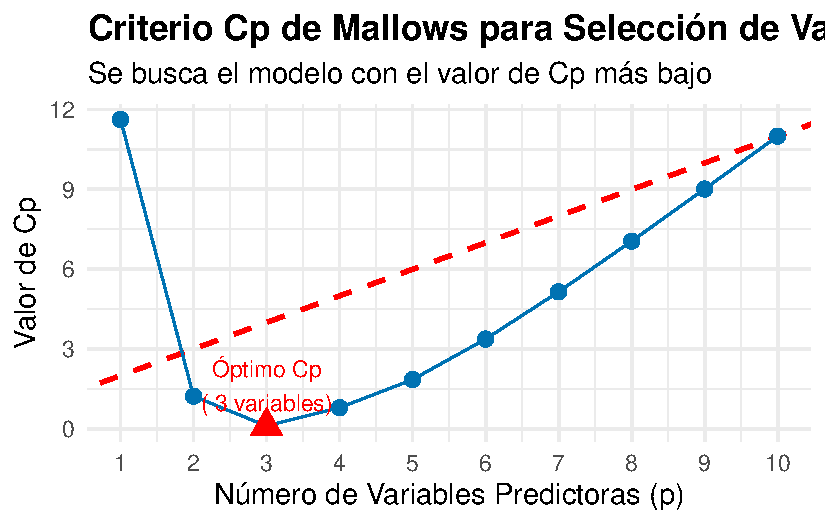
\includegraphics[keepaspectratio]{tema4_files/figure-pdf/cp-mallows-grafico-1.pdf}}

\begin{Shaded}
\begin{Highlighting}[]
\CommentTok{\# 5. Mostrar las variables del modelo seleccionado}
\NormalTok{variables\_mejor\_modelo\_cp }\OtherTok{\textless{}{-}} \FunctionTok{names}\NormalTok{(}\FunctionTok{which}\NormalTok{(subset\_summary}\SpecialCharTok{$}\NormalTok{which[mejor\_cp\_idx, }\SpecialCharTok{{-}}\DecValTok{1}\NormalTok{]))}
\end{Highlighting}
\end{Shaded}

El gráfico resultante nos permite diagnosticar visualmente la calidad de
los modelos candidatos. La línea discontinua roja representa la
referencia para un modelo sin sesgo (\(C_p = p+1\)).

La estrategia de selección es clara: \textbf{identificar el modelo que
minimice el estadístico Cp}. Este punto representa el mejor equilibrio
teórico entre el sesgo del modelo (subajuste) y su varianza
(sobreajuste). La línea roja nos ayuda a confirmar visualmente que el
modelo elegido, además de ser el de menor Cp, tiene un sesgo bajo.

Como se observa, el estadístico Cp disminuye drásticamente al pasar de
uno a dos predictores. El modelo con \textbf{3 variables} es el
seleccionado como óptimo porque alcanza el valor de Cp más bajo de todos
los candidatos, con un valor de \textbf{0.1}.

El análisis sugiere que el modelo más parsimonioso y con el mejor
rendimiento predictivo se compone de las siguientes variables:
\textbf{wt, qsec, am}. Añadir más predictores más allá de este punto
óptimo no mejora el modelo; de hecho, el valor de Cp comienza a
aumentar, lo que indica que estamos añadiendo una complejidad
innecesaria y empezando a sobreajustar los datos.

\end{tcolorbox}

\subsection{¿Cuándo Usar Cada
Criterio?}\label{cuuxe1ndo-usar-cada-criterio}

La existencia de varios criterios plantea una pregunta natural: ¿cuál
debemos usar? La respuesta depende en gran medida del objetivo final de
nuestro análisis.

Si el \textbf{objetivo principal es la predicción}, el \textbf{AIC}
suele ser la opción preferida. Su diseño para minimizar el error de
predicción lo hace ideal en contextos de pronóstico, donde el
rendimiento en datos nuevos es lo más importante. Su penalización más
moderada permite incluir variables que, aunque no sean ``verdaderas'' en
un sentido causal, ayudan a mejorar la precisión de las predicciones.

Por otro lado, si el \textbf{objetivo es la explicación o la inferencia}
---es decir, identificar el modelo más parsimonioso que probablemente
representa el verdadero proceso generador de los datos---, el
\textbf{BIC} es la elección más sólida. Su penalización más fuerte
protege de forma más robusta contra el sobreajuste y, en muestras
grandes, su propiedad de consistencia le da una base teórica más fuerte
para la selección del ``modelo verdadero''.

El \textbf{Cp de Mallows} es especialmente valioso en un contexto más
exploratorio, cuando queremos entender explícitamente el compromiso
entre el sesgo y la varianza. Al graficar \(C_p\) frente a \(p+1\) para
diferentes subconjuntos de modelos, podemos visualizar claramente el
punto en el que añadir más variables deja de reducir el sesgo y solo
empieza a inflar la varianza, ofreciendo una visión muy clara del
``codo'' de complejidad óptima.

Es común que estos criterios no coincidan en su selección. Cuando esto
ocurre, no debe verse como un fracaso, sino como una indicación de que
no existe un único modelo ``mejor'' de forma inequívoca. En tales casos,
el juicio del analista es clave, y se pueden usar herramientas
adicionales como la \textbf{validación cruzada}
(\emph{cross-validation}) para comparar el rendimiento predictivo de los
modelos finalistas y tomar una decisión informada.

\begin{tcolorbox}[enhanced jigsaw, leftrule=.75mm, breakable, colbacktitle=quarto-callout-important-color!10!white, bottomrule=.15mm, colframe=quarto-callout-important-color-frame, toprule=.15mm, colback=white, coltitle=black, bottomtitle=1mm, left=2mm, title=\textcolor{quarto-callout-important-color}{\faExclamation}\hspace{0.5em}{El Principio de Parsimonia en la Selección de Modelos}, opacityback=0, arc=.35mm, opacitybacktitle=0.6, toptitle=1mm, titlerule=0mm, rightrule=.15mm]

El \textbf{principio de parsimonia}, también conocido como la ``navaja
de Occam'', es un concepto fundamental que subyace a todos los criterios
de bondad de ajuste. Este principio establece que, entre modelos que
explican igualmente bien un fenómeno, \textbf{se debe preferir el más
simple}.

\end{tcolorbox}

\section{Métodos de selección
exhaustiva}\label{muxe9todos-de-selecciuxf3n-exhaustiva}

Los métodos de selección exhaustiva son un enfoque fundamental en la
búsqueda de un subconjunto óptimo de variables predictoras en modelos de
regresión. Este enfoque evalúa de manera sistemática diferentes
combinaciones de variables para identificar cuál de ellas proporciona el
mejor ajuste al modelo en función de un criterio predefinido, como el
coeficiente de determinación ajustado (\(R^2\) ajustado) o criterios de
información como AIC o BIC.

A diferencia de los métodos automáticos, los métodos de selección
exhaustiva no dependen de un proceso iterativo de adición o eliminación
de variables. En cambio, buscan exhaustivamente (o mediante
aproximaciones computacionalmente más eficientes) entre todas las
posibles combinaciones de variables, lo que garantiza un análisis
completo de las interacciones y relevancias potenciales.

El método más conocido dentro de este enfoque es la \textbf{selección
del mejor subconjunto (Best Subset Selection)}, que evalúa todos los
subconjuntos posibles de variables y selecciona el mejor para cada
tamaño específico. Es el enfoque más completo pero también el más
exigente computacionalmente. Para un conjunto de \(p\) variables
predictoras, este método construye todos los modelos posibles que
incluyen \(k\) variables, donde \(k = 1, 2, ..., p\), seleccionando el
mejor modelo de cada tamaño según el criterio elegido.

\begin{tcolorbox}[enhanced jigsaw, leftrule=.75mm, breakable, colbacktitle=quarto-callout-tip-color!10!white, bottomrule=.15mm, colframe=quarto-callout-tip-color-frame, toprule=.15mm, colback=white, coltitle=black, bottomtitle=1mm, left=2mm, title=\textcolor{quarto-callout-tip-color}{\faLightbulb}\hspace{0.5em}{Ejemplo de selección exhaustiva}, opacityback=0, arc=.35mm, opacitybacktitle=0.6, toptitle=1mm, titlerule=0mm, rightrule=.15mm]

\begin{Shaded}
\begin{Highlighting}[]
\CommentTok{\# Ejemplo de Best Subset Selection maximizando R² ajustado}
\FunctionTok{suppressPackageStartupMessages}\NormalTok{(}\FunctionTok{library}\NormalTok{(leaps))}

\CommentTok{\# Usando el dataset mtcars}
\FunctionTok{data}\NormalTok{(mtcars)}

\CommentTok{\# Realizar best subset selection}
\NormalTok{best\_subset }\OtherTok{\textless{}{-}} \FunctionTok{regsubsets}\NormalTok{(mpg }\SpecialCharTok{\textasciitilde{}}\NormalTok{ ., }\AttributeTok{data =}\NormalTok{ mtcars, }\AttributeTok{nvmax =} \DecValTok{10}\NormalTok{)}

\CommentTok{\# Obtener estadísticas del mejor modelo según R² ajustado}
\NormalTok{subset\_summary }\OtherTok{\textless{}{-}} \FunctionTok{summary}\NormalTok{(best\_subset)}
\NormalTok{mejor\_modelo\_idx }\OtherTok{\textless{}{-}} \FunctionTok{which.max}\NormalTok{(subset\_summary}\SpecialCharTok{$}\NormalTok{adjr2)}
\NormalTok{mejor\_r2\_adj }\OtherTok{\textless{}{-}} \FunctionTok{max}\NormalTok{(subset\_summary}\SpecialCharTok{$}\NormalTok{adjr2)}
\NormalTok{total\_variables }\OtherTok{\textless{}{-}} \FunctionTok{ncol}\NormalTok{(mtcars) }\SpecialCharTok{{-}} \DecValTok{1}  \CommentTok{\# Excluir variable respuesta}
\NormalTok{variables\_seleccionadas }\OtherTok{\textless{}{-}}\NormalTok{ mejor\_modelo\_idx}
\end{Highlighting}
\end{Shaded}

El método de selección exhaustiva aplicado al conjunto de datos
\texttt{mtcars} identifica el modelo óptimo que maximiza el R² ajustado.
Este modelo alcanza un \textbf{R² ajustado de 0.8375}, utilizando
\textbf{5 variables} del total de \textbf{10 variables} predictoras
disponibles. Esta selección representa un equilibrio óptimo entre la
capacidad explicativa del modelo y la penalización por complejidad,
demostrando cómo la evaluación exhaustiva puede identificar el
subconjunto de variables que mejor explica la variabilidad en el consumo
de combustible.

\end{tcolorbox}

Esta aproximación presenta importantes \textbf{ventajas}: garantiza
encontrar el mejor subconjunto según el criterio elegido (optimalidad
garantizada), examina todas las posibles combinaciones de variables
ofreciendo una evaluación completa, y proporciona un estándar sólido
para comparar otros métodos de selección. Sin embargo, también tiene
\textbf{limitaciones} significativas: la complejidad computacional crece
exponencialmente ya que con \(p\) variables se generan \(2^p\) modelos
posibles, lo que hace que sea impracticable para \(p\) grande
(típicamente \(p > 15-20\)). Además, sin una validación cruzada
adecuada, puede seleccionar modelos sobreajustados.

Estos métodos son especialmente útiles cuando el número de predictores
no es demasiado grande, ya que el esfuerzo computacional crece
exponencialmente con el número de variables. Aunque el costo
computacional puede ser elevado en datasets amplios, los métodos de
selección exhaustiva proporcionan una referencia sólida y transparente
para evaluar qué variables son fundamentales en el modelo, siendo
particularmente valiosos en estudios donde la interpretabilidad y la
certeza sobre la selección de variables son prioritarias.

¡Perfecto! El texto que tienes es una excelente introducción. Ahora
vamos a expandir cada uno de esos puntos para darles la profundidad
teórica y práctica que necesitan en el libro, explicando el algoritmo de
cada método, sus criterios de decisión y sus ventajas y limitaciones.

Aquí tienes una propuesta para desarrollar esa sección.

\section{Métodos automáticos paso a
paso}\label{muxe9todos-automuxe1ticos-paso-a-paso}

Los métodos automáticos de selección de variables, a menudo llamados
métodos secuenciales o por pasos (\emph{stepwise}), son algoritmos
diseñados para explorar el espacio de posibles modelos de una manera
computacionalmente eficiente. A diferencia del método de mejores
subconjuntos (\emph{best subset selection}), que evalúa todos los
modelos posibles, estos enfoques siguen un camino restringido, añadiendo
o quitando predictores de uno en uno.

El principio clave es construir un modelo de forma iterativa, tomando en
cada paso una decisión ``localmente óptima'' basada en un criterio
estadístico. Los criterios más comunes son el p-valor de un predictor, o
el cambio que este produce en un indicador global como el \textbf{AIC},
el \textbf{BIC} o el \textbf{\(R^2\) ajustado}.

\subsection{Selección progresiva (Forward
Selection)}\label{selecciuxf3n-progresiva-forward-selection}

Esta estrategia es la más intuitiva: parte de la nada y construye el
modelo pieza por pieza, añadiendo en cada paso el predictor que aporta
la mayor mejora.

\textbf{El Algoritmo}

\begin{enumerate}
\def\labelenumi{\arabic{enumi}.}
\tightlist
\item
  \textbf{Inicio}: Se comienza con el \textbf{modelo nulo}, que solo
  contiene el intercepto (\(Y \sim 1\)).
\item
  \textbf{Primer Paso}: Se ajustan \(p\) modelos de regresión simple,
  uno para cada una de las \(p\) variables predictoras disponibles. Se
  elige la variable que mejor explica la respuesta (la que tiene el
  p-valor más bajo en su test t, o la que produce el AIC/BIC más bajo).
  Esta variable se convierte en el primer predictor del modelo.
\item
  \textbf{Pasos Siguientes}: Se ajustan \(p-1\) nuevos modelos, cada uno
  de los cuales contiene la(s) variable(s) ya seleccionada(s) más una de
  las variables restantes. De nuevo, se selecciona y se añade la
  variable que produce la mayor mejora en el criterio elegido.
\item
  \textbf{Finalización}: El proceso se repite y se detiene cuando
  ninguna de las variables restantes mejora el modelo de forma
  significativa al ser añadida (por ejemplo, ninguna tiene un p-valor
  por debajo de un umbral predefinido, o el AIC/BIC del modelo deja de
  disminuir).
\end{enumerate}

\textbf{Ventajas y Limitaciones}

\begin{itemize}
\tightlist
\item
  \textbf{Ventaja}: Es computacionalmente muy eficiente. Puede aplicarse
  en situaciones con un número de predictores muy grande, incluso cuando
  hay más predictores que observaciones (\(p > n\)).
\item
  \textbf{Limitación}: Su principal debilidad es su \textbf{``miopía''}.
  Una variable seleccionada en una etapa temprana se queda en el modelo
  para siempre. Sin embargo, es posible que esa variable se vuelva
  redundante una vez que se añadan otros predictores. El método
  \emph{forward} no puede rectificar decisiones pasadas, por lo que no
  garantiza encontrar el mejor modelo posible.
\end{itemize}

\subsection{Eliminación regresiva (Backward
Elimination)}\label{eliminaciuxf3n-regresiva-backward-elimination}

Esta estrategia adopta el enfoque opuesto: empieza con todo y va
eliminando lo que no es útil, como un escultor que retira el mármol
sobrante.

\textbf{El Algoritmo}

\begin{enumerate}
\def\labelenumi{\arabic{enumi}.}
\tightlist
\item
  \textbf{Inicio}: Se comienza con el \textbf{modelo completo}, que
  incluye todas las \(p\) variables predictoras disponibles
  (\(Y \sim X_1 + X_2 + \dots + X_p\)).
\item
  \textbf{Primer Paso}: Se ajusta el modelo completo y se examina la
  significancia de cada predictor. Se identifica la variable
  \textbf{menos significativa}, es decir, aquella con el p-valor más
  alto en su test t (o la que, al ser eliminada, produce la menor
  disminución en la calidad del modelo según AIC/BIC).
\item
  \textbf{Pasos Siguientes}: Si el p-valor de esa variable supera un
  umbral de permanencia (p.~ej., \(\alpha_{out} = 0.10\)), se elimina
  del modelo. A continuación, se vuelve a ajustar el modelo con las
  \(p-1\) variables restantes.
\item
  \textbf{Finalización}: El proceso de identificar y eliminar la
  variable menos significativa se repite hasta que todas las variables
  que quedan en el modelo son estadísticamente significativas (es decir,
  todas tienen un p-valor por debajo del umbral de permanencia).
\end{enumerate}

\textbf{Ventajas y Limitaciones}

\begin{itemize}
\tightlist
\item
  \textbf{Ventaja}: Generalmente se considera superior al método
  \emph{forward} porque empieza evaluando el efecto de cada variable en
  presencia de todas las demás. Esto proporciona un contexto inicial más
  completo.
\item
  \textbf{Limitación}: No se puede utilizar si el número de predictores
  es mayor que el número de observaciones (\(p > n\)), ya que es
  imposible ajustar el modelo completo inicial. Además, al igual que el
  método \emph{forward}, una vez que una variable es eliminada, no puede
  volver a entrar, lo que podría llevar a eliminar por error una
  variable que es importante en combinación con un subconjunto más
  pequeño de predictores.
\end{itemize}

\subsection{Selección paso a paso (Stepwise
Regression)}\label{selecciuxf3n-paso-a-paso-stepwise-regression}

Este método es un híbrido que intenta combinar lo mejor de las dos
estrategias anteriores, permitiendo un proceso de ``prueba y error'' más
flexible.

\textbf{El Algoritmo}

La selección \emph{stepwise} es esencialmente una selección
\emph{forward} con un añadido crucial: en cada paso, después de añadir
una nueva variable, se realiza una \textbf{verificación hacia atrás}
para comprobar si alguna de las variables que ya estaban en el modelo se
ha vuelto redundante.

\begin{enumerate}
\def\labelenumi{\arabic{enumi}.}
\tightlist
\item
  \textbf{Paso Adelante (Forward)}: Al igual que en la selección
  progresiva, se añade la variable que más mejora el modelo.
\item
  \textbf{Paso Atrás (Backward)}: Después de añadir esa variable, se
  examinan \textbf{todas las variables ya incluidas} en el modelo. Si
  alguna de ellas ha perdido su significancia (su p-valor ha aumentado
  por encima de un umbral de eliminación), se elimina.
\item
  \textbf{Repetición}: El proceso continúa, alternando pasos hacia
  adelante y hacia atrás, hasta que se alcanza un punto de equilibrio en
  el que ninguna variable puede ser añadida ni eliminada según los
  umbrales establecidos.
\end{enumerate}

\textbf{Ventajas y Limitaciones}

\begin{itemize}
\tightlist
\item
  \textbf{Ventaja}: Es más robusto que los métodos \emph{forward} o
  \emph{backward} puros, ya que puede corregir decisiones anteriores.
  Una variable que fue importante al principio puede ser eliminada más
  tarde si otra la hace redundante.
\item
  \textbf{Limitación}: A pesar de su flexibilidad, sigue siendo un
  algoritmo ``codicioso'' (\emph{greedy}) que no explora todo el espacio
  de modelos. Por tanto, tampoco garantiza encontrar el mejor modelo
  global.
\end{itemize}

\begin{tcolorbox}[enhanced jigsaw, leftrule=.75mm, breakable, colbacktitle=quarto-callout-warning-color!10!white, bottomrule=.15mm, colframe=quarto-callout-warning-color-frame, toprule=.15mm, colback=white, coltitle=black, bottomtitle=1mm, left=2mm, title=\textcolor{quarto-callout-warning-color}{\faExclamationTriangle}\hspace{0.5em}{Advertencia sobre los métodos automáticos}, opacityback=0, arc=.35mm, opacitybacktitle=0.6, toptitle=1mm, titlerule=0mm, rightrule=.15mm]

Aunque estos métodos son herramientas útiles para un primer cribado de
variables, deben usarse con extrema cautela. Su naturaleza automática
puede llevar a conclusiones erróneas si no se supervisan con criterio.

\begin{enumerate}
\def\labelenumi{\arabic{enumi}.}
\tightlist
\item
  \textbf{No garantizan el mejor modelo}: Al seguir un camino fijo,
  pueden pasar por alto el subconjunto de variables verdaderamente
  óptimo.
\item
  \textbf{Invalidez de los p-valores}: Los p-valores, errores estándar e
  intervalos de confianza del modelo final están \textbf{sesgados} y son
  excesivamente optimistas. El proceso de selección ha ``elegido a los
  ganadores'' de antemano, y la teoría de la inferencia estándar no se
  aplica a un modelo que ha sido seleccionado de esta manera.
\item
  \textbf{Inestabilidad}: Los resultados pueden ser muy sensibles a
  pequeñas variaciones en los datos. Añadir o quitar unas pocas
  observaciones puede cambiar drásticamente el modelo seleccionado.
\end{enumerate}

Por estas razones, los métodos automáticos deben considerarse como
\textbf{herramientas exploratorias} para generar modelos candidatos, no
como un procedimiento definitivo. La selección final siempre debe estar
guiada por el conocimiento del dominio, la teoría subyacente y un
diagnóstico riguroso.

\end{tcolorbox}

\section{Métodos basados en
regularización}\label{muxe9todos-basados-en-regularizaciuxf3n}

En los modelos de regresión, especialmente cuando se trabaja con un gran
número de variables predictoras o con datos multicolineales, los métodos
tradicionales de selección de variables pueden resultar ineficaces o
inestables. En estos casos, los métodos basados en regularización surgen
como una alternativa poderosa que no solo selecciona variables, sino que
también mejora la estabilidad y la precisión del modelo.

La regularización consiste en introducir una penalización en la función
de ajuste del modelo, lo que tiene dos efectos principales: controlar el
sobreajuste al reducir la complejidad del modelo y forzar la selección
de un subconjunto más parsimonioso de predictores. Estas penalizaciones
ajustan los coeficientes de las variables predictoras, favoreciendo
soluciones más simples y robustas (James et al. 2013).

Entre los métodos de regularización más destacados se encuentran:

\begin{itemize}
\tightlist
\item
  \textbf{Ridge Regression:} Aplica una penalización proporcional al
  cuadrado de los coeficientes, lo que permite manejar problemas de
  multicolinealidad pero no conduce a la eliminación completa de
  variables.
\item
  \textbf{Lasso (Least Absolute Shrinkage and Selection Operator):}
  Introduce una penalización basada en el valor absoluto de los
  coeficientes, lo que no solo reduce su magnitud, sino que también
  puede anularlos completamente, realizando una selección automática de
  variables.
\item
  \textbf{Elastic Net:} Combina las penalizaciones de Ridge y Lasso,
  ofreciendo mayor flexibilidad en situaciones donde hay una gran
  correlación entre los predictores.
\end{itemize}

Estos métodos son especialmente útiles en problemas donde el número de
variables predictoras excede el número de observaciones, o cuando se
desea un modelo más interpretable. En esta sección, exploraremos en
detalle los fundamentos teóricos, la implementación práctica y las
aplicaciones de cada uno de estos métodos, destacando sus ventajas en
escenarios complejos y desafiantes.

\subsection{Ridge regression}\label{ridge-regression}

La regresión Ridge introduce una penalización en la estimación de los
coeficientes de regresión, lo que ayuda a reducir la varianza del modelo
y mejora su capacidad predictiva en presencia de datos altamente
correlacionados o con muchas variables (Marquardt and Snee 1975). El
modelo de regresión Ridge es una extensión de la regresión lineal
estándar. Con datos observados, escribimos:

\[
\mathbf{y}= \mathbf{X} \, \boldsymbol{\beta} + \boldsymbol{\varepsilon}
\]

donde:

\begin{itemize}
\tightlist
\item
  \(\mathbf{y}\) es el vector de respuesta observado de dimensión
  \(n \times 1\).
\item
  \(\mathbf{X}\) es la matriz de diseño observada de dimensión
  \(n \times (p+1)\) (la primera columna suele ser de unos para el
  intercepto).
\item
  \(\boldsymbol{\beta} = (\beta_0, \beta_1, \dots, \beta_p)^T\) es el
  vector de coeficientes.
\item
  \(\boldsymbol{\varepsilon}\) es el vector de errores.
\end{itemize}

En mínimos cuadrados ordinarios (OLS), los coeficientes se estiman
minimizando la suma de los errores al cuadrado:

\[
SSE = \sum_{i=1}^{n} (y_i - \hat{y}_i)^2 = \| 
\mathbf{y} - \mathbf{X} \, \boldsymbol{\beta} \|^2.
\]

Sin embargo, cuando hay multicolinealidad, la matriz
\(\mathbf{X}^T \mathbf{X}\) puede ser casi singular, generando
coeficientes inestables. Para evitar esto, la regresión Ridge añade un
\textbf{término de penalización} \(\lambda\), de la siguiente manera
(sin penalizar el intercepto \(\beta_0\)):

\[
SSE_{ridge} = \| \mathbf{y} - \mathbf{X} \, \boldsymbol{\beta} \|^2 + \lambda \sum_{j=1}^{p} \beta_j^2.
\]

Este término adicional, es un \textbf{término de penalización}
(\(L_2=\sum \beta_j^2\)) impone una restricción sobre los coeficientes,
evitando que tomen valores excesivamente grandes. La estimación de
\(\boldsymbol{\beta}\) en Ridge se obtiene resolviendo:

\[
\hat{\boldsymbol{\beta}}_{\text{ridge}} = (\mathbf{X}^T \mathbf{X} + \lambda \, \mathbf{P})^{-1} 
\mathbf{X}^T \mathbf{y}.
\]

donde \(\mathbf{P}\) es diagonal con \(P_{11}=0\) (no penalizamos el
intercepto) y \(P_{jj}=1\) para \(j=2,\dots,p+1\), y \(\lambda \geq 0\)
controla la cantidad de penalización aplicada. (Cuando no hay intercepto
o se reparametriza, a menudo se escribe con \(I\) para simplificar.)

\textbf{Interpretación del parámetro} \(\lambda\)

\begin{itemize}
\tightlist
\item
  Si \(\lambda = 0\), el modelo Ridge es equivalente a la regresión
  lineal tradicional (OLS).
\item
  A medida que \(\lambda\) aumenta, los coeficientes \(\beta_j\)
  (pendientes) se reducen en magnitud, lo que ayuda a controlar la
  varianza del modelo y a prevenir el sobreajuste.
\item
  Si \(\lambda\) es demasiado grande, los coeficientes se acercan a cero
  y el modelo puede perder interpretabilidad.
\end{itemize}

La elección óptima de \(\lambda\) se determina generalmente mediante
\textbf{validación cruzada}.

\begin{tcolorbox}[enhanced jigsaw, leftrule=.75mm, breakable, colbacktitle=quarto-callout-caution-color!10!white, bottomrule=.15mm, colframe=quarto-callout-caution-color-frame, toprule=.15mm, colback=white, coltitle=black, bottomtitle=1mm, left=2mm, title=\textcolor{quarto-callout-caution-color}{\faFire}\hspace{0.5em}{Aviso}, opacityback=0, arc=.35mm, opacitybacktitle=0.6, toptitle=1mm, titlerule=0mm, rightrule=.15mm]

Los detalles de la validación cruzada son tratados en la asignatura de
Minería de Datos.

\end{tcolorbox}

\begin{tcolorbox}[enhanced jigsaw, leftrule=.75mm, breakable, colbacktitle=quarto-callout-note-color!10!white, bottomrule=.15mm, colframe=quarto-callout-note-color-frame, toprule=.15mm, colback=white, coltitle=black, bottomtitle=1mm, left=2mm, title=\textcolor{quarto-callout-note-color}{\faInfo}\hspace{0.5em}{Propiedades Clave}, opacityback=0, arc=.35mm, opacitybacktitle=0.6, toptitle=1mm, titlerule=0mm, rightrule=.15mm]

\begin{itemize}
\item
  \textbf{Manejo de la multicolinealidad:} La regularización reduce la
  sensibilidad del modelo cuando los predictores están altamente
  correlacionados.
\item
  \textbf{Menor varianza en las predicciones:} El modelo Ridge tiende a
  ser más estable en comparación con OLS, lo que mejora la capacidad de
  generalización en conjuntos de datos nuevos.
\item
  \textbf{No realiza selección de variables:} A diferencia de Lasso,
  Ridge \textbf{no anula coeficientes}, sino que reduce su magnitud.
  Esto es útil cuando se sospecha que todas las variables tienen algún
  grado de importancia en el modelo.
\end{itemize}

\end{tcolorbox}

\begin{tcolorbox}[enhanced jigsaw, leftrule=.75mm, breakable, colbacktitle=quarto-callout-tip-color!10!white, bottomrule=.15mm, colframe=quarto-callout-tip-color-frame, toprule=.15mm, colback=white, coltitle=black, bottomtitle=1mm, left=2mm, title=\textcolor{quarto-callout-tip-color}{\faLightbulb}\hspace{0.5em}{Ejemplo}, opacityback=0, arc=.35mm, opacitybacktitle=0.6, toptitle=1mm, titlerule=0mm, rightrule=.15mm]

\begin{Shaded}
\begin{Highlighting}[]
\CommentTok{\# Cargar librerías}
\FunctionTok{suppressPackageStartupMessages}\NormalTok{(}\FunctionTok{library}\NormalTok{(glmnet))}

\CommentTok{\# Datos simulados}
\FunctionTok{set.seed}\NormalTok{(}\DecValTok{123}\NormalTok{)}
\NormalTok{X }\OtherTok{\textless{}{-}} \FunctionTok{matrix}\NormalTok{(}\FunctionTok{rnorm}\NormalTok{(}\DecValTok{100} \SpecialCharTok{*} \DecValTok{10}\NormalTok{), }\DecValTok{100}\NormalTok{, }\DecValTok{10}\NormalTok{)  }\CommentTok{\# 100 observaciones, 10 predictores}
\NormalTok{Y }\OtherTok{\textless{}{-}}\NormalTok{ X }\SpecialCharTok{\%*\%} \FunctionTok{rnorm}\NormalTok{(}\DecValTok{10}\NormalTok{) }\SpecialCharTok{+} \FunctionTok{rnorm}\NormalTok{(}\DecValTok{100}\NormalTok{)  }\CommentTok{\# Variable de respuesta con ruido}

\CommentTok{\# Ajustar modelo Ridge}
\NormalTok{modelo\_ridge }\OtherTok{\textless{}{-}} \FunctionTok{glmnet}\NormalTok{(X, Y, }\AttributeTok{alpha =} \DecValTok{0}\NormalTok{)  }\CommentTok{\# alpha = 0 indica regresión Ridge}

\CommentTok{\# Seleccionar lambda óptimo con validación cruzada}
\NormalTok{cv\_ridge }\OtherTok{\textless{}{-}} \FunctionTok{cv.glmnet}\NormalTok{(X, Y, }\AttributeTok{alpha =} \DecValTok{0}\NormalTok{)}
\NormalTok{lambda\_optimo }\OtherTok{\textless{}{-}}\NormalTok{ cv\_ridge}\SpecialCharTok{$}\NormalTok{lambda.min  }\CommentTok{\# Mejor valor de lambda}

\FunctionTok{print}\NormalTok{(lambda\_optimo)}
\end{Highlighting}
\end{Shaded}

\begin{verbatim}
[1] 0.2583753
\end{verbatim}

\begin{Shaded}
\begin{Highlighting}[]
\CommentTok{\# Ajustar modelo final con lambda óptimo}
\NormalTok{modelo\_ridge\_final }\OtherTok{\textless{}{-}} \FunctionTok{glmnet}\NormalTok{(X, Y, }\AttributeTok{alpha =} \DecValTok{0}\NormalTok{, }\AttributeTok{lambda =}\NormalTok{ lambda\_optimo)}

\NormalTok{modelo\_ridge\_final}
\end{Highlighting}
\end{Shaded}

\begin{verbatim}

Call:  glmnet(x = X, y = Y, alpha = 0, lambda = lambda_optimo) 

  Df  %Dev Lambda
1 10 93.55 0.2584
\end{verbatim}

\begin{Shaded}
\begin{Highlighting}[]
\CommentTok{\# Comparación modelo clásico}

\NormalTok{modelo\_lm }\OtherTok{\textless{}{-}} \FunctionTok{lm}\NormalTok{(Y}\SpecialCharTok{\textasciitilde{}}\NormalTok{X)}

\CommentTok{\# Mostrar coeficientes}
\NormalTok{output}\OtherTok{=}\FunctionTok{cbind}\NormalTok{(}\FunctionTok{round}\NormalTok{(}\FunctionTok{coef}\NormalTok{(modelo\_ridge\_final),}\DecValTok{3}\NormalTok{),}
            \FunctionTok{round}\NormalTok{(}\FunctionTok{coef}\NormalTok{(modelo\_lm),}\DecValTok{3}\NormalTok{))}

\FunctionTok{colnames}\NormalTok{(output)}\OtherTok{=}\FunctionTok{c}\NormalTok{(}\StringTok{"RIDGE"}\NormalTok{,}\StringTok{"OLS"}\NormalTok{)}

\NormalTok{output}
\end{Highlighting}
\end{Shaded}

\begin{verbatim}
11 x 2 sparse Matrix of class "dgCMatrix"
             RIDGE    OLS
(Intercept)  0.118  0.132
V1          -0.874 -0.995
V2          -1.019 -1.131
V3           0.040  0.039
V4           0.002  0.001
V5          -2.500 -2.703
V6           1.001  1.104
V7           0.247  0.274
V8           2.125  2.244
V9           0.635  0.658
V10         -0.390 -0.427
\end{verbatim}

\end{tcolorbox}

La regresión Ridge es una técnica poderosa para mejorar la estabilidad
de los modelos de regresión en presencia de multicolinealidad. A
diferencia de OLS, que puede generar coeficientes inestables, Ridge
introduce una penalización que reduce la magnitud de los coeficientes,
evitando valores extremos. Aunque Ridge no realiza selección de
variables, su capacidad para reducir la varianza y mejorar la capacidad
predictiva lo convierte en una herramienta esencial en el análisis de
datos modernos.

En la siguiente sección, exploraremos la \textbf{regresión Lasso}, que
extiende este concepto permitiendo la eliminación de variables
irrelevantes del modelo.

\subsection{Regresión Lasso}\label{regresiuxf3n-lasso}

Cuando se tiene un conjunto de predictores con posibles redundancias o
ruido, Lasso permite identificar cuáles son las variables más relevantes
para el modelo, lo que facilita la interpretación y reduce la
complejidad del análisis.

Al igual que en Ridge, el modelo de regresión Lasso se define sobre
datos observados mediante la minimización (Ranstam and Cook 2018): \[
SSE_{\text{lasso}} = \| \mathbf{y} - \mathbf{X} \, \boldsymbol{\beta} \|^2 + \lambda \sum_{j=1}^{p} |\beta_j|
\]

donde el \textbf{término de penalización} (\(L_1=\sum |\beta_j|\)) no
penaliza el intercepto \(\beta_0\) y hace que algunos coeficientes de
pendiente se reduzcan exactamente a \textbf{cero}, eliminando variables
del modelo.

La diferencia clave con \textbf{Ridge Regressión}, visto anteriormente,
es que Ridge reduce la magnitud de los coeficientes pero no los anula,
mientras que \textbf{Lasso puede eliminar variables por completo}.

\textbf{Interpretación del parámetro} \(\lambda\)

\begin{itemize}
\tightlist
\item
  Si \(\lambda = 0\), el modelo es equivalente a la regresión lineal
  tradicional (OLS).
\item
  A medida que \(\lambda\) aumenta, más coeficientes de pendiente se
  reducen a cero, lo que equivale a realizar \textbf{selección de
  variables}.
\item
  Si \(\lambda\) es demasiado grande, se eliminan demasiadas variables,
  lo que puede resultar en un modelo subóptimo.
\end{itemize}

Al igual que en el método \emph{Ridge}, la selección óptima de
\(\lambda\) se realiza generalmente mediante \textbf{validación
cruzada}.

\begin{tcolorbox}[enhanced jigsaw, leftrule=.75mm, breakable, colbacktitle=quarto-callout-note-color!10!white, bottomrule=.15mm, colframe=quarto-callout-note-color-frame, toprule=.15mm, colback=white, coltitle=black, bottomtitle=1mm, left=2mm, title=\textcolor{quarto-callout-note-color}{\faInfo}\hspace{0.5em}{Propiedades Clave}, opacityback=0, arc=.35mm, opacitybacktitle=0.6, toptitle=1mm, titlerule=0mm, rightrule=.15mm]

\begin{itemize}
\tightlist
\item
  \textbf{Selección de variables automática:} Lasso no solo regulariza,
  sino que también selecciona las variables más importantes eliminando
  aquellas menos relevantes.
\item
  \textbf{Manejo de la multicolinealidad:} Puede mejorar la
  interpretación del modelo cuando hay muchas variables correlacionadas.
\item
  \textbf{Simplicidad y interpretabilidad:} Un modelo con menos
  variables es más fácil de interpretar y aplicar en la práctica.
\item
  \textbf{Reduce el sobreajuste:} La penalización \(L_1\) evita que el
  modelo se ajuste demasiado a los datos de entrenamiento, mejorando su
  capacidad predictiva en datos nuevos.
\end{itemize}

\end{tcolorbox}

\begin{tcolorbox}[enhanced jigsaw, leftrule=.75mm, breakable, colbacktitle=quarto-callout-tip-color!10!white, bottomrule=.15mm, colframe=quarto-callout-tip-color-frame, toprule=.15mm, colback=white, coltitle=black, bottomtitle=1mm, left=2mm, title=\textcolor{quarto-callout-tip-color}{\faLightbulb}\hspace{0.5em}{Ejemplo}, opacityback=0, arc=.35mm, opacitybacktitle=0.6, toptitle=1mm, titlerule=0mm, rightrule=.15mm]

\begin{Shaded}
\begin{Highlighting}[]
\CommentTok{\# Ajustar modelo Lasso}
\NormalTok{modelo\_lasso }\OtherTok{\textless{}{-}} \FunctionTok{glmnet}\NormalTok{(X, Y, }\AttributeTok{alpha =} \DecValTok{1}\NormalTok{)  }\CommentTok{\# alpha = 1 indica regresión Lasso}

\CommentTok{\# Seleccionar lambda óptimo con validación cruzada}
\NormalTok{cv\_lasso }\OtherTok{\textless{}{-}} \FunctionTok{cv.glmnet}\NormalTok{(X, Y, }\AttributeTok{alpha =} \DecValTok{1}\NormalTok{)}
\NormalTok{lambda\_optimo }\OtherTok{\textless{}{-}}\NormalTok{ cv\_lasso}\SpecialCharTok{$}\NormalTok{lambda.min  }\CommentTok{\# Mejor valor de lambda}

\FunctionTok{print}\NormalTok{(lambda\_optimo)}
\end{Highlighting}
\end{Shaded}

\begin{verbatim}
[1] 0.03260326
\end{verbatim}

\begin{Shaded}
\begin{Highlighting}[]
\CommentTok{\# Ajustar modelo final con lambda óptimo}
\NormalTok{modelo\_lasso\_final }\OtherTok{\textless{}{-}} \FunctionTok{glmnet}\NormalTok{(X, Y, }\AttributeTok{alpha =} \DecValTok{1}\NormalTok{, }\AttributeTok{lambda =}\NormalTok{ lambda\_optimo)}


\CommentTok{\# Mostrar coeficientes}
\NormalTok{output}\OtherTok{=}\FunctionTok{cbind}\NormalTok{(}\FunctionTok{round}\NormalTok{(}\FunctionTok{coef}\NormalTok{(modelo\_lasso\_final),}\DecValTok{3}\NormalTok{),output)}

\FunctionTok{colnames}\NormalTok{(output)}\OtherTok{=}\FunctionTok{c}\NormalTok{(}\StringTok{"LASSO"}\NormalTok{,}\StringTok{"RIDGE"}\NormalTok{,}\StringTok{"OLS"}\NormalTok{)}

\NormalTok{output}
\end{Highlighting}
\end{Shaded}

\begin{verbatim}
11 x 3 sparse Matrix of class "dgCMatrix"
             LASSO  RIDGE    OLS
(Intercept)  0.131  0.118  0.132
V1          -0.950 -0.874 -0.995
V2          -1.078 -1.019 -1.131
V3           0.006  0.040  0.039
V4           .      0.002  0.001
V5          -2.652 -2.500 -2.703
V6           1.058  1.001  1.104
V7           0.235  0.247  0.274
V8           2.213  2.125  2.244
V9           0.629  0.635  0.658
V10         -0.392 -0.390 -0.427
\end{verbatim}

\end{tcolorbox}

\textbf{Consideraciones Importantes}

La regresión Lasso es una poderosa técnica de regularización que no solo
mejora la estabilidad del modelo en presencia de muchas variables
predictoras, sino que también realiza una selección automática de las
más relevantes. Su capacidad para reducir coeficientes a cero la
convierte en una herramienta esencial en el análisis de datos de alta
dimensión.

\begin{itemize}
\tightlist
\item
  \textbf{Lasso puede eliminar demasiadas variables si} \(\lambda\) es
  demasiado grande, lo que puede llevar a la pérdida de información
  importante.
\item
  \textbf{No maneja bien grupos de predictores altamente
  correlacionados}, ya que selecciona solo uno de ellos y elimina los
  demás.
\item
  \textbf{Elastic Net}, que combina Ridge y Lasso, puede ser una mejor
  opción cuando hay \textbf{multicolinealidad fuerte} en los datos.
\end{itemize}

En la siguiente sección, exploraremos \textbf{Elastic Net}, una técnica
híbrida que combina las ventajas de Ridge y Lasso para mejorar la
selección de variables en presencia de predictores altamente
correlacionados.

\subsection{Elastic Net}\label{elastic-net}

La regresión \textbf{Elastic Net} es una técnica de regularización que
combina las propiedades de \textbf{Ridge} y \textbf{Lasso}, abordando
algunas de sus limitaciones individuales (Zou and Hastie 2005). Mientras
que Ridge es útil para manejar la multicolinealidad sin eliminar
variables y Lasso selecciona un subconjunto de predictores, Elastic Net
equilibra ambos enfoques permitiendo la selección de variables en
presencia de alta correlación entre los predictores.

Este método es particularmente efectivo cuando el número de predictores
es grande y existe \textbf{multicolinealidad}, ya que permite controlar
simultáneamente la \textbf{reducción de la magnitud de los coeficientes}
y la \textbf{eliminación de variables irrelevantes}.

Elastic Net introduce una penalización que combina los términos de Ridge
(\(L_2\)) y Lasso (\(L_1\)), sobre datos observados:

\[
SSE_{\text{Elastic Net}} = \| \mathbf{y} - \mathbf{X} \, \boldsymbol{\beta} \|^2 + \lambda_1 \sum_{j=1}^{p} |\beta_j| + \lambda_2 \sum_{j=1}^{p} \beta_j^2 \]

donde:

\begin{itemize}
\tightlist
\item
  \(\lambda_1\) (asociado a Lasso) controla la cantidad de coeficientes
  que se reducen a \textbf{cero}.
\item
  \(\lambda_2\) (asociado a Ridge) controla la \textbf{reducción de
  magnitud} de los coeficientes sin anularlos.
\item
  \(\alpha\) es un parámetro adicional que pondera la combinación entre
  Lasso y Ridge, con:

  \begin{itemize}
  \tightlist
  \item
    \(\alpha = 1\) → Elastic Net se comporta como Lasso.
  \item
    \(\alpha = 0\) → Elastic Net se comporta como Ridge.
  \item
    \(0 < \alpha < 1\) → Elastic Net combina ambos métodos.
  \end{itemize}
\end{itemize}

La estimación de los coeficientes en Elastic Net se obtiene resolviendo
(habitualmente sin penalizar el intercepto):

\[
\hat{\boldsymbol{\beta}}_{\text{EN}} = \arg \min_{\boldsymbol{\beta}} \left( \| \mathbf{y} - \mathbf{X} \, \boldsymbol{\beta} \|^2 + \lambda \left( \alpha \sum_{j=1}^{p} |\beta_j| + (1 - \alpha) \sum_{j=1}^{p} \beta_j^2 \right) \right)
\]

\begin{tcolorbox}[enhanced jigsaw, leftrule=.75mm, breakable, colbacktitle=quarto-callout-note-color!10!white, bottomrule=.15mm, colframe=quarto-callout-note-color-frame, toprule=.15mm, colback=white, coltitle=black, bottomtitle=1mm, left=2mm, title=\textcolor{quarto-callout-note-color}{\faInfo}\hspace{0.5em}{Propiedades Clave}, opacityback=0, arc=.35mm, opacitybacktitle=0.6, toptitle=1mm, titlerule=0mm, rightrule=.15mm]

\begin{itemize}
\item
  \textbf{Manejo de la Multicolinealidad:} A diferencia de Lasso, que
  selecciona solo una de las variables correlacionadas y elimina las
  demás, Elastic Net distribuye la penalización entre todas las
  variables correlacionadas, evitando una selección arbitraria.
\item
  \textbf{Selección de variables más estable:} La combinación de Lasso y
  Ridge permite una selección más robusta, manteniendo información
  relevante del modelo sin eliminar predictores clave.
\item
  \textbf{Mejora del rendimiento predictivo:} Al utilizar validación
  cruzada para seleccionar los hiperparámetros \(\lambda_1\),
  \(\lambda_2\) y \(\alpha\), se optimiza la capacidad del modelo para
  generalizar a nuevos datos.
\end{itemize}

\end{tcolorbox}

\begin{tcolorbox}[enhanced jigsaw, leftrule=.75mm, breakable, colbacktitle=quarto-callout-tip-color!10!white, bottomrule=.15mm, colframe=quarto-callout-tip-color-frame, toprule=.15mm, colback=white, coltitle=black, bottomtitle=1mm, left=2mm, title=\textcolor{quarto-callout-tip-color}{\faLightbulb}\hspace{0.5em}{Ejemplo}, opacityback=0, arc=.35mm, opacitybacktitle=0.6, toptitle=1mm, titlerule=0mm, rightrule=.15mm]

\begin{Shaded}
\begin{Highlighting}[]
\CommentTok{\# Ajustar modelo Elastic Net}
\NormalTok{modelo\_elastic\_net }\OtherTok{\textless{}{-}} \FunctionTok{glmnet}\NormalTok{(X, Y, }\AttributeTok{alpha =} \FloatTok{0.5}\NormalTok{)  }\CommentTok{\# Alpha = 0.5 (50\% Ridge, 50\% Lasso)}

\CommentTok{\# Seleccionar lambda óptimo con validación cruzada}
\NormalTok{cv\_elastic\_net }\OtherTok{\textless{}{-}} \FunctionTok{cv.glmnet}\NormalTok{(X, Y, }\AttributeTok{alpha =} \FloatTok{0.5}\NormalTok{)}
\NormalTok{lambda\_optimo }\OtherTok{\textless{}{-}}\NormalTok{ cv\_elastic\_net}\SpecialCharTok{$}\NormalTok{lambda.min  }\CommentTok{\# Mejor valor de lambda}

\FunctionTok{print}\NormalTok{(lambda\_optimo)}
\end{Highlighting}
\end{Shaded}

\begin{verbatim}
[1] 0.0213522
\end{verbatim}

\begin{Shaded}
\begin{Highlighting}[]
\CommentTok{\# Ajustar modelo final con lambda óptimo}
\NormalTok{modelo\_elastic\_final }\OtherTok{\textless{}{-}} \FunctionTok{glmnet}\NormalTok{(X, Y, }\AttributeTok{alpha =} \FloatTok{0.5}\NormalTok{, }\AttributeTok{lambda =}\NormalTok{ lambda\_optimo)}

\CommentTok{\# Mostrar coeficientes}
\NormalTok{output}\OtherTok{=}\FunctionTok{cbind}\NormalTok{(}\FunctionTok{round}\NormalTok{(}\FunctionTok{coef}\NormalTok{(modelo\_elastic\_final),}\DecValTok{3}\NormalTok{),output)}

\FunctionTok{colnames}\NormalTok{(output)}\OtherTok{=}\FunctionTok{c}\NormalTok{(}\StringTok{"ELASTIC"}\NormalTok{,}\StringTok{"LASSO"}\NormalTok{,}\StringTok{"RIDGE"}\NormalTok{,}\StringTok{"OLS"}\NormalTok{)}

\NormalTok{output}
\end{Highlighting}
\end{Shaded}

\begin{verbatim}
11 x 4 sparse Matrix of class "dgCMatrix"
            ELASTIC  LASSO  RIDGE    OLS
(Intercept)   0.131  0.131  0.118  0.132
V1           -0.975 -0.950 -0.874 -0.995
V2           -1.108 -1.078 -1.019 -1.131
V3            0.028  0.006  0.040  0.039
V4            .      .      0.002  0.001
V5           -2.677 -2.652 -2.500 -2.703
V6            1.084  1.058  1.001  1.104
V7            0.260  0.235  0.247  0.274
V8            2.229  2.213  2.125  2.244
V9            0.647  0.629  0.635  0.658
V10          -0.414 -0.392 -0.390 -0.427
\end{verbatim}

\end{tcolorbox}

Para determinar el mejor valor de \(\alpha\), se usa \textbf{validación
cruzada} probando distintos valores entre \(0\) y 1. Algunas estrategias
comunes incluyen:

\begin{itemize}
\tightlist
\item
  \textbf{Si hay muchas variables irrelevantes}, se recomienda
  \(\alpha\) cercano a 1 (Lasso).
\item
  \textbf{Si hay fuerte multicolinealidad}, se recomienda \(\alpha\)
  cercano a 0 (Ridge).
\item
  \textbf{Si se desea un balance entre selección y estabilidad}, se
  suele usar \(\alpha = 0.5\).
\end{itemize}

La regresión Elastic Net combina lo mejor de Ridge y Lasso, ofreciendo
un método de regularización robusto para modelos con muchas variables
predictoras y posible multicolinealidad. Su capacidad para seleccionar
variables sin eliminar información clave lo convierte en una opción
ideal para modelos complejos y de alta dimensionalidad.

\subsection{Comparación de los métodos de
Regularización}\label{comparaciuxf3n-de-los-muxe9todos-de-regularizaciuxf3n}

\begin{longtable}[]{@{}
  >{\raggedright\arraybackslash}p{(\linewidth - 4\tabcolsep) * \real{0.3333}}
  >{\raggedright\arraybackslash}p{(\linewidth - 4\tabcolsep) * \real{0.3333}}
  >{\raggedright\arraybackslash}p{(\linewidth - 4\tabcolsep) * \real{0.3333}}@{}}
\toprule\noalign{}
\begin{minipage}[b]{\linewidth}\raggedright
Método
\end{minipage} & \begin{minipage}[b]{\linewidth}\raggedright
Penalización
\end{minipage} & \begin{minipage}[b]{\linewidth}\raggedright
Efecto sobre los coeficientes
\end{minipage} \\
\midrule\noalign{}
\endhead
\bottomrule\noalign{}
\endlastfoot
\textbf{OLS} & Ninguna & Sin restricción, puede haber
multicolinealidad \\
\textbf{Ridge} & \(L_2\) & Reduce la magnitud de los coeficientes, pero
no los anula \\
\textbf{Lasso} & \(L_1\) & Puede anular coeficientes, permitiendo
selección de variables \\
\textbf{Elastic Net} & \(L_1 + L_2\) & Combinación de Ridge y Lasso \\
\end{longtable}

\begin{center}\rule{0.5\linewidth}{0.5pt}\end{center}

Lasso es especialmente útil cuando se sospecha que muchas variables son
irrelevantes, mientras que Ridge es preferido cuando se espera que todas
las variables aporten información al modelo.

Elastic Net es ideal cuando hay \textbf{muchas variables
correlacionadas} y se desea un modelo \textbf{estable y parsimonioso}.

\begin{itemize}
\item
  Elastic Net mejora la estabilidad del modelo en comparación con Lasso,
  especialmente cuando hay variables predictoras altamente
  correlacionadas.
\item
  Es más flexible que Ridge y Lasso individualmente, permitiendo un
  ajuste más fino a distintos tipos de problemas.
\item
  Requiere la selección de hiperparámetros (\(\lambda\) y \(\alpha\)),
  por lo que debe usarse validación cruzada para encontrar la
  combinación óptima.
\end{itemize}

\section{Validación del Modelo}\label{validaciuxf3n-del-modelo}

Hemos ajustado un modelo, interpretado sus coeficientes y evaluado su
significancia estadística. Pero, ¿cómo podemos estar seguros de que
funcionará bien en el futuro, con datos que nunca ha visto? Esta es la
pregunta fundamental que la \textbf{validación del modelo} busca
responder.

Imagina que estás preparando un examen. Si solo memorizas las respuestas
de los exámenes de años anteriores (tus \textbf{datos de
entrenamiento}), puede que saques una nota perfecta en ellos. Sin
embargo, cuando te enfrentes al examen real con preguntas nuevas (los
\textbf{datos de prueba}), es probable que tu rendimiento sea
decepcionante. Esto, en esencia, es el \textbf{sobreajuste}
(\emph{overfitting}): un modelo que se aprende los datos de
entrenamiento ``de memoria'', incluyendo su ruido y peculiaridades, pero
que pierde su capacidad de \textbf{generalizar} a nuevas observaciones.

La validación es el proceso de simular este ``examen final'' para
obtener una estimación honesta del rendimiento predictivo de nuestro
modelo en el mundo real (James et al. 2013). Se compone de dos elementos
clave: las \textbf{estrategias de validación}, que nos dicen cómo
simular el examen, y las \textbf{métricas de evaluación}, que nos dicen
cómo calificarlo.

\subsection{Estrategias de
Validación}\label{estrategias-de-validaciuxf3n}

Para evaluar la capacidad de generalización, necesitamos probar el
modelo en datos que no se usaron para entrenarlo. Las siguientes
estrategias nos permiten hacer precisamente eso.

\begin{tcolorbox}[enhanced jigsaw, leftrule=.75mm, breakable, colbacktitle=quarto-callout-warning-color!10!white, bottomrule=.15mm, colframe=quarto-callout-warning-color-frame, toprule=.15mm, colback=white, coltitle=black, bottomtitle=1mm, left=2mm, title=\textcolor{quarto-callout-warning-color}{\faExclamationTriangle}\hspace{0.5em}{El primer paso no negociable: La partición inicial}, opacityback=0, arc=.35mm, opacitybacktitle=0.6, toptitle=1mm, titlerule=0mm, rightrule=.15mm]

Antes de escribir una sola línea de código para ajustar un modelo,
seleccionar variables o ejecutar una validación cruzada, el
procedimiento \textbf{siempre} debe comenzar con una única acción:

\textbf{Dividir el conjunto de datos completo en dos partes y guardar
una de ellas bajo llave.}

\begin{enumerate}
\def\labelenumi{\arabic{enumi}.}
\tightlist
\item
  \textbf{Datos de modelado (p.~ej., 80\% del total):} Este es el
  conjunto de datos con el que trabajarás. Lo usarás para todas tus
  tareas de construcción y evaluación de modelos: entrenar, comparar
  diferentes conjuntos de variables, y ejecutar estrategias como la
  validación cruzada.
\item
  \textbf{Conjunto de prueba Final (p.~ej., 20\% restante):} Este
  conjunto de datos debe ser guardado y \textbf{no ser utilizado bajo
  ninguna circunstancia} durante el proceso de modelado. Es tu ``examen
  final sorpresa'', tu única oportunidad de obtener una estimación
  verdaderamente honesta y no sesgada del rendimiento del modelo que has
  seleccionado como el campeón definitivo.
\end{enumerate}

La validación cruzada y la división simple train/test que veremos a
continuación son técnicas que se aplican \textbf{dentro} de los ``datos
de modelado''.

\end{tcolorbox}

\subsubsection{El Conjunto de entrenamiento y test (Train/Test
Split)}\label{el-conjunto-de-entrenamiento-y-test-traintest-split}

La estrategia más directa es tomar nuestros ``Datos de Modelado'' (el
80\% inicial) y volver a dividirlos, creando un único ``examen'' para el
proceso de construcción del modelo (Hastie et al. 2009):

\begin{enumerate}
\def\labelenumi{\arabic{enumi}.}
\tightlist
\item
  \textbf{Conjunto de entrenamiento (\emph{Training Set})}: Usualmente,
  el 70-80\% de los datos. El modelo se construye y se ajusta usando
  únicamente esta porción. Es aquí donde el modelo ``aprende''.
\item
  \textbf{Conjunto de test (\emph{Test Set})}: El 20-30\% restante.
  Estos datos se mantienen ``ocultos'' durante el entrenamiento. Una vez
  que el modelo está finalizado, lo usamos para predecir la variable
  respuesta en este conjunto. La comparación entre las predicciones
  (\(\hat{y}\)) y los valores reales (\(y\)) nos da una medida no
  sesgada de su rendimiento.
\end{enumerate}

Aunque es simple y computacionalmente barata, esta técnica tiene una
debilidad importante: los resultados pueden depender mucho de la
división aleatoria específica que se haya hecho. Si por mala suerte en
el conjunto de prueba caen observaciones muy atípicas, nuestra
evaluación del modelo será excesivamente pesimista. Si caen puntos muy
fáciles de predecir, será demasiado optimista. Esta alta variabilidad es
un problema, especialmente con muestras de datos pequeñas.

\subsubsection{Validación cruzada
(Cross-Validation)}\label{validaciuxf3n-cruzada-cross-validation}

La \textbf{validación cruzada} es la solución a la variabilidad de la
división simple y se aplica, de nuevo, \textbf{sobre el conjunto total
de ``datos de modelado''}. En lugar de hacer un único ``examen final'',
la validación cruzada promedia los resultados de múltiples
mini-exámenes, proporcionando una estimación del error mucho más estable
y fiable (James et al. 2013).

El método más común es la \textbf{validación cruzada de k-particiones
(\emph{k-fold cross-validation})}. Su nombre describe el proceso: los
datos se dividen en \emph{k} particiones y se ``cruzan'' los roles de
entrenamiento y validación.

El resultado final de este procedimiento es el \textbf{error de
validación cruzada}, que se calcula promediando los errores obtenidos en
cada una de las \emph{k} particiones. Esto nos da una única métrica de
rendimiento para el modelo.

\[CV_{(k)} = \frac{1}{k}\sum_{i=1}^{k} \text{Métrica}_i\]

donde \(\text{Métrica}_i\) es la métrica de error (como RMSE o MAE)
calculada en la i-ésima iteración. La elección de \emph{k} suele ser 5 o
10, ya que se ha demostrado que estos valores ofrecen un buen equilibrio
entre el sesgo y la varianza de la estimación del error.

\begin{tcolorbox}[enhanced jigsaw, leftrule=.75mm, breakable, colbacktitle=quarto-callout-note-color!10!white, bottomrule=.15mm, colframe=quarto-callout-note-color-frame, toprule=.15mm, colback=white, coltitle=black, bottomtitle=1mm, left=2mm, title=\textcolor{quarto-callout-note-color}{\faInfo}\hspace{0.5em}{Procedimiento de k-particiones}, opacityback=0, arc=.35mm, opacitybacktitle=0.6, toptitle=1mm, titlerule=0mm, rightrule=.15mm]

\begin{enumerate}
\def\labelenumi{\arabic{enumi}.}
\tightlist
\item
  \textbf{División}: Dividir aleatoriamente los datos en \emph{k}
  \textbf{particiones} de tamaño similar.
\item
  \textbf{Iteración}: Para cada partición \(i = 1, 2, ..., k\):

  \begin{itemize}
  \tightlist
  \item
    Usar la partición \(i\) como conjunto de test.
  \item
    Usar las restantes \(k-1\) particiones como conjunto de
    entrenamiento.
  \item
    Ajustar el modelo y calcular las métricas de desempeño en el
    conjunto de test.
  \end{itemize}
\item
  \textbf{Promedio}: Calcular el promedio de las métricas a través de
  las \emph{k} iteraciones.
\end{enumerate}

\end{tcolorbox}

Un caso extremo de este método es la \textbf{validación cruzada
``dejando uno fuera'' (LOOCV)}, donde \emph{k} es igual al número de
observaciones, \emph{n}. En cada iteración, se entrena el modelo con
\emph{n-1} datos y se prueba en el único punto restante. Aunque es
computacionalmente muy costoso, en regresión lineal existe una
afortunada fórmula matemática que nos permite calcular el error LOOCV
con la misma rapidez que un solo ajuste:

\[CV_{(n)} = \frac{1}{n}\sum_{i=1}^{n}\left(\frac{y_i - \hat{y}_i}{1-h_{ii}}\right)^2\]

donde \(h_{ii}\) es el apalancamiento (\emph{leverage}) de la i-ésima
observación.

\begin{tcolorbox}[enhanced jigsaw, leftrule=.75mm, breakable, colbacktitle=quarto-callout-important-color!10!white, bottomrule=.15mm, colframe=quarto-callout-important-color-frame, toprule=.15mm, colback=white, coltitle=black, bottomtitle=1mm, left=2mm, title=\textcolor{quarto-callout-important-color}{\faExclamation}\hspace{0.5em}{Guía para seleccionar estrategia de validación}, opacityback=0, arc=.35mm, opacitybacktitle=0.6, toptitle=1mm, titlerule=0mm, rightrule=.15mm]

\textbf{Usa Train/Test cuando:}

\begin{itemize}
\tightlist
\item
  El dataset es grande (n \textgreater{} 1000)
\item
  Los recursos computacionales son limitados\\
\item
  Se requiere una evaluación rápida
\end{itemize}

\textbf{Usa validación cruzada k-fold cuando:}

\begin{itemize}
\tightlist
\item
  El dataset es de tamaño moderado (n \textless{} 1000)
\item
  Se requiere una estimación más estable del desempeño
\item
  Se dispone de recursos computacionales adecuados
\end{itemize}

\textbf{Usa LOOCV cuando:}

\begin{itemize}
\tightlist
\item
  El dataset es pequeño (n \textless{} 100)
\item
  Se requiere la estimación menos sesgada posible
\item
  El tiempo computacional no es una restricción crítica
\end{itemize}

\end{tcolorbox}

\subsection{Métricas de rendimiento}\label{muxe9tricas-de-rendimiento}

Una vez que usamos una estrategia de validación para generar
predicciones sobre datos no vistos, necesitamos una ``nota'' para
cuantificar qué tan buenos fueron esos pronósticos. Aquí es donde entran
las métricas de error.

\subsubsection{Raíz del error cuadrático
medio}\label{rauxedz-del-error-cuadruxe1tico-medio}

La métrica más utilizada es la \textbf{raíz del error cuadrático medio
(RMSE)}. Es como una desviación típica de los residuos, y nos da una
idea de la magnitud promedio de los errores de predicción.

\[RMSE = \sqrt{\frac{1}{n}\sum_{i=1}^{n}(y_i - \hat{y}_i)^2}\]

La característica clave del RMSE es que, al elevar los errores al
cuadrado, \textbf{penaliza de forma desproporcionada los errores
grandes}. Un solo error de predicción de 10 unidades contribuye al RMSE
mucho más que 10 errores de 1 unidad. Esto lo hace muy sensible a
valores atípicos. Su gran ventaja es que se expresa en las mismas
unidades que la variable respuesta, facilitando su interpretación.

\subsubsection{Error absoluto medio}\label{error-absoluto-medio}

Una alternativa popular es el \textbf{error absoluto medio (MAE)}, que
simplemente promedia el valor absoluto de los errores.

\[MAE = \frac{1}{n}\sum_{i=1}^{n}|y_i - \hat{y}_i|\]

A diferencia del RMSE, el MAE no eleva los errores al cuadrado, por lo
que \textbf{trata todos los errores de forma proporcional a su
magnitud}. Un error de 10 unidades es simplemente el doble de malo que
un error de 5. Esto hace que el MAE sea \textbf{más robusto frente a
valores atípicos} y, para muchos, más fácil de interpretar como ``el
error promedio'' que cometemos en nuestras predicciones.

En resumen, la validación nos obliga a confrontar nuestro modelo con la
realidad de datos nuevos. Usando una estrategia robusta como la
\textbf{validación cruzada} para calcular una métrica interpretable como
el \textbf{RMSE} o el \textbf{MAE}, podemos obtener una estimación
fiable de su rendimiento predictivo y construir modelos en los que
realmente podamos confiar. Claro, aquí tienes ese contenido reorganizado
y resumido dentro de un recuadro (\texttt{callout}), ideal para destacar
esta idea clave en tu libro.

\begin{tcolorbox}[enhanced jigsaw, leftrule=.75mm, breakable, colbacktitle=quarto-callout-important-color!10!white, bottomrule=.15mm, colframe=quarto-callout-important-color-frame, toprule=.15mm, colback=white, coltitle=black, bottomtitle=1mm, left=2mm, title=\textcolor{quarto-callout-important-color}{\faExclamation}\hspace{0.5em}{Interpretando el Error}, opacityback=0, arc=.35mm, opacitybacktitle=0.6, toptitle=1mm, titlerule=0mm, rightrule=.15mm]

La comparación entre el error del modelo en los datos que ha visto
(entrenamiento) y en datos que no ha visto (validación) es la
herramienta de diagnóstico más importante para entender el ajuste del
modelo.

La regla general es que el error de entrenamiento siempre será más bajo
(más optimista) que el de test. La clave está en analizar la
\textbf{diferencia} entre ambos.

\textbf{Sobreajuste (Overfitting)}

\begin{itemize}
\tightlist
\item
  \textbf{Síntoma}: Error de entrenamiento \textbf{bajo} + Error de test
  \textbf{mucho más alto}.
\item
  \textbf{Diagnóstico}: El modelo ha ``memorizado'' el ruido de los
  datos de entrenamiento y no es capaz de generalizar a nuevos datos.
\item
  \textbf{Solución}: Simplificar el modelo (usar menos variables,
  aplicar regularización como Ridge o Lasso).
\end{itemize}

\textbf{Subajuste (Underfitting)}

\begin{itemize}
\tightlist
\item
  \textbf{Síntoma}: Error de entrenamiento \textbf{alto} + Error de test
  \textbf{alto y similar}.
\item
  \textbf{Diagnóstico}: El modelo es demasiado simple y no tiene la
  capacidad de capturar la estructura subyacente de los datos.
\item
  \textbf{Solución}: Aumentar la complejidad del modelo (añadir más
  variables, incluir interacciones o términos no lineales).
\end{itemize}

\end{tcolorbox}

\begin{tcolorbox}[enhanced jigsaw, leftrule=.75mm, breakable, colbacktitle=quarto-callout-tip-color!10!white, bottomrule=.15mm, colframe=quarto-callout-tip-color-frame, toprule=.15mm, colback=white, coltitle=black, bottomtitle=1mm, left=2mm, title=\textcolor{quarto-callout-tip-color}{\faLightbulb}\hspace{0.5em}{La maldición del sobreajuste}, opacityback=0, arc=.35mm, opacitybacktitle=0.6, toptitle=1mm, titlerule=0mm, rightrule=.15mm]

Para ilustrar por qué la validación es indispensable, realizaremos un
experimento controlado. Crearemos un conjunto de datos donde
\textbf{conocemos la verdad}: sabemos exactamente qué variables influyen
en la respuesta y cuáles son puro ruido. Luego, compararemos dos
modelos:

\begin{enumerate}
\def\labelenumi{\arabic{enumi}.}
\tightlist
\item
  \textbf{Modelo Completo}: Un modelo que incluye todas las variables
  disponibles, tanto las útiles como las de ruido.
\item
  \textbf{Modelo Correcto}: Un modelo que incluye únicamente las
  variables que realmente tienen un efecto sobre la respuesta.
\end{enumerate}

El objetivo es ver cuál de los dos modelos predice mejor en datos ``no
vistos'', utilizando la validación cruzada para simular este escenario.

\textbf{1. Simulación de Datos}

Creamos un dataset con 100 observaciones. La variable \texttt{y}
dependerá de \texttt{X1}, \texttt{X2} y \texttt{X3}. Las variables
\texttt{X4} a \texttt{X10} no tendrán ninguna relación real con
\texttt{y}; serán \textbf{predictores de ruido}.

\begin{Shaded}
\begin{Highlighting}[]
\CommentTok{\# Cargar la librería \textquotesingle{}caret\textquotesingle{}, que simplifica enormemente el proceso de validación}
\FunctionTok{suppressPackageStartupMessages}\NormalTok{(}\FunctionTok{library}\NormalTok{(caret))}

\CommentTok{\# Para reproducibilidad}
\FunctionTok{set.seed}\NormalTok{(}\DecValTok{42}\NormalTok{)}

\CommentTok{\# Crear datos de ejemplo}
\NormalTok{n }\OtherTok{\textless{}{-}} \DecValTok{100}
\CommentTok{\# 3 predictores verdaderos y 7 de ruido}
\NormalTok{X }\OtherTok{\textless{}{-}} \FunctionTok{matrix}\NormalTok{(}\FunctionTok{rnorm}\NormalTok{(n }\SpecialCharTok{*} \DecValTok{10}\NormalTok{), n, }\DecValTok{10}\NormalTok{)}
\FunctionTok{colnames}\NormalTok{(X) }\OtherTok{\textless{}{-}} \FunctionTok{paste0}\NormalTok{(}\StringTok{"X"}\NormalTok{, }\DecValTok{1}\SpecialCharTok{:}\DecValTok{10}\NormalTok{)}

\CommentTok{\# La respuesta \textquotesingle{}y\textquotesingle{} depende SOLO de X1, X2 y X3}
\NormalTok{beta\_true }\OtherTok{\textless{}{-}} \FunctionTok{c}\NormalTok{(}\FloatTok{2.5}\NormalTok{, }\SpecialCharTok{{-}}\FloatTok{1.5}\NormalTok{, }\DecValTok{3}\NormalTok{, }\DecValTok{0}\NormalTok{, }\DecValTok{0}\NormalTok{, }\DecValTok{0}\NormalTok{, }\DecValTok{0}\NormalTok{, }\DecValTok{0}\NormalTok{, }\DecValTok{0}\NormalTok{, }\DecValTok{0}\NormalTok{) }
\NormalTok{y }\OtherTok{\textless{}{-}}\NormalTok{ X }\SpecialCharTok{\%*\%}\NormalTok{ beta\_true }\SpecialCharTok{+} \FunctionTok{rnorm}\NormalTok{(n, }\AttributeTok{sd =} \DecValTok{2}\NormalTok{)}

\CommentTok{\# Combinar en un data frame}
\NormalTok{datos }\OtherTok{\textless{}{-}} \FunctionTok{data.frame}\NormalTok{(}\AttributeTok{y =}\NormalTok{ y, X)}

\NormalTok{indices\_modelado }\OtherTok{\textless{}{-}} \FunctionTok{createDataPartition}\NormalTok{(datos}\SpecialCharTok{$}\NormalTok{y, }\AttributeTok{p =} \FloatTok{0.8}\NormalTok{, }\AttributeTok{list =} \ConstantTok{FALSE}\NormalTok{)}
\NormalTok{datos\_modelado }\OtherTok{\textless{}{-}}\NormalTok{ datos[indices\_modelado, ]}
\NormalTok{datos\_prueba\_final }\OtherTok{\textless{}{-}}\NormalTok{ datos[}\SpecialCharTok{{-}}\NormalTok{indices\_modelado, ]}
\end{Highlighting}
\end{Shaded}

\textbf{2. Ajuste y Evaluación de Modelos con Validación Cruzada}

Usaremos la función \texttt{train()} del paquete \texttt{caret}, que es
una herramienta increíblemente potente para ajustar y validar modelos.
Configuraremos una \textbf{validación cruzada de 10 particiones (10-fold
CV)} para estimar el error de predicción (RMSE) de nuestros dos modelos.

\begin{Shaded}
\begin{Highlighting}[]
\CommentTok{\# Configurar el método de validación cruzada de 10 particiones}
\NormalTok{control\_cv }\OtherTok{\textless{}{-}} \FunctionTok{trainControl}\NormalTok{(}\AttributeTok{method =} \StringTok{"cv"}\NormalTok{, }\AttributeTok{number =} \DecValTok{10}\NormalTok{)}

\CommentTok{\# Ajustar y validar el MODELO COMPLETO (incluye predictores de ruido)}
\NormalTok{modelo\_completo }\OtherTok{\textless{}{-}} \FunctionTok{train}\NormalTok{(}
\NormalTok{  y }\SpecialCharTok{\textasciitilde{}}\NormalTok{ ., }
  \AttributeTok{data =}\NormalTok{ datos\_modelado, }
  \AttributeTok{method =} \StringTok{"lm"}\NormalTok{,}
  \AttributeTok{trControl =}\NormalTok{ control\_cv}
\NormalTok{)}

\CommentTok{\# Ajustar y validar el MODELO CORRECTO (solo los predictores relevantes)}
\NormalTok{modelo\_correcto }\OtherTok{\textless{}{-}} \FunctionTok{train}\NormalTok{(}
\NormalTok{  y }\SpecialCharTok{\textasciitilde{}}\NormalTok{ X1 }\SpecialCharTok{+}\NormalTok{ X2 }\SpecialCharTok{+}\NormalTok{ X3, }
  \AttributeTok{data =}\NormalTok{ datos\_modelado, }
  \AttributeTok{method =} \StringTok{"lm"}\NormalTok{,}
  \AttributeTok{trControl =}\NormalTok{ control\_cv}
\NormalTok{)}

\CommentTok{\# Comparar los resultados de la validación cruzada de ambos modelos}
\NormalTok{resultados\_cv }\OtherTok{\textless{}{-}} \FunctionTok{resamples}\NormalTok{(}\FunctionTok{list}\NormalTok{(}\AttributeTok{COMPLETO =}\NormalTok{ modelo\_completo, }\AttributeTok{CORRECTO =}\NormalTok{ modelo\_correcto))}
\NormalTok{resumen\_cv }\OtherTok{\textless{}{-}} \FunctionTok{summary}\NormalTok{(resultados\_cv)}
\NormalTok{resumen\_cv}
\end{Highlighting}
\end{Shaded}

\begin{verbatim}

Call:
summary.resamples(object = resultados_cv)

Models: COMPLETO, CORRECTO 
Number of resamples: 10 

MAE 
              Min.  1st Qu.   Median     Mean  3rd Qu.     Max. NA's
COMPLETO 0.8638906 1.284897 1.585880 1.685953 1.895840 2.783321    0
CORRECTO 0.7192667 1.279226 1.602489 1.687326 2.283342 2.477780    0

RMSE 
              Min.  1st Qu.   Median     Mean  3rd Qu.     Max. NA's
COMPLETO 1.0722692 1.592663 2.105678 2.116903 2.523848 3.119017    0
CORRECTO 0.9052294 1.474694 1.934304 2.020464 2.480041 3.124041    0

Rsquared 
              Min.   1st Qu.    Median      Mean   3rd Qu.      Max. NA's
COMPLETO 0.5917775 0.7793610 0.8556182 0.8189137 0.8882997 0.9505874    0
CORRECTO 0.5019737 0.7988599 0.8513481 0.8017851 0.9048191 0.9385882    0
\end{verbatim}

\begin{Shaded}
\begin{Highlighting}[]
\CommentTok{\# Extraer métricas RMSE para uso en el texto}
\NormalTok{rmse\_correcto }\OtherTok{\textless{}{-}} \FunctionTok{round}\NormalTok{(resumen\_cv}\SpecialCharTok{$}\NormalTok{statistics}\SpecialCharTok{$}\NormalTok{RMSE[}\StringTok{"CORRECTO"}\NormalTok{, }\StringTok{"Mean"}\NormalTok{], }\DecValTok{3}\NormalTok{)}
\NormalTok{rmse\_completo }\OtherTok{\textless{}{-}} \FunctionTok{round}\NormalTok{(resumen\_cv}\SpecialCharTok{$}\NormalTok{statistics}\SpecialCharTok{$}\NormalTok{RMSE[}\StringTok{"COMPLETO"}\NormalTok{, }\StringTok{"Mean"}\NormalTok{], }\DecValTok{3}\NormalTok{)}
\end{Highlighting}
\end{Shaded}

\textbf{3. Análisis de Resultados}

Al comparar el \textbf{RMSE} promedio obtenido en la validación cruzada,
la conclusión es clara: el \textbf{Modelo Correcto} (2.02) es
consistentemente \textbf{mejor} (menor error) que el \textbf{Modelo
Completo} (2.117).

El \textbf{Modelo Completo} sufre de \textbf{sobreajuste}. Al incluir
las 7 variables de ruido, se esfuerza por encontrar patrones en datos
puramente aleatorios. ``Aprende'' estas relaciones falsas en los datos
de entrenamiento, pero falla al predecir en datos nuevos. El
\textbf{Modelo Correcto}, al ser más parsimonioso, captura la estructura
fundamental y generaliza mejor.

Este ejemplo demuestra la lección más importante del modelado:
\textbf{un buen ajuste en los datos de entrenamiento no garantiza un
buen rendimiento predictivo}. La validación es el único método fiable
para estimar la verdadera calidad de un modelo.

\textbf{4. El Veredicto Final en el Conjunto de Prueba}

La validación cruzada nos ha servido como un juez imparcial para
comparar nuestros modelos candidatos y seleccionar el
\texttt{Modelo\ Correcto} como el claro ganador. Ahora, para obtener una
estimación final y no sesgada de su rendimiento en el mundo real,
tomamos ese modelo elegido y lo enfrentamos a los
\texttt{datos\_prueba\_final}, el conjunto de datos que ha permanecido
intacto durante todo el proceso.

\begin{Shaded}
\begin{Highlighting}[]
\CommentTok{\# Usamos el modelo ganador (modelo\_correcto) para predecir sobre los datos de prueba}
\NormalTok{predicciones\_finales }\OtherTok{\textless{}{-}} \FunctionTok{predict}\NormalTok{(modelo\_correcto, }\AttributeTok{newdata =}\NormalTok{ datos\_prueba\_final)}

\CommentTok{\# Calculamos el RMSE final comparando las predicciones con los valores reales de prueba}
\NormalTok{rmse\_final }\OtherTok{\textless{}{-}} \FunctionTok{RMSE}\NormalTok{(predicciones\_finales, datos\_prueba\_final}\SpecialCharTok{$}\NormalTok{y)}
\end{Highlighting}
\end{Shaded}

Al evaluar nuestro modelo final, obtenemos un RMSE en el conjunto de
prueba de \textbf{1.966}.

Este valor es nuestra estimación más honesta del error de predicción que
podemos esperar de nuestro modelo al enfrentarse a nuevos datos. Es
crucial compararlo con el error que estimamos durante la validación
cruzada (2.02). El hecho de que ambos valores sean muy similares
confirma que nuestro proceso de validación fue robusto y que no hemos
sobreajustado el modelo al conjunto de datos de modelado. Este RMSE
final es el que reportaríamos como la medida definitiva del rendimiento
predictivo de nuestro modelo.

\end{tcolorbox}

\bookmarksetup{startatroot}

\chapter{Modelos de regresión generalizada}\label{sec-tema4}

Hasta ahora hemos estuadiado la regresión lineal como una herramienta
poderosa para modelar la relación entre una variable dependiente
continua y un conjunto de variables independientes. Sin embargo, en
muchos contextos del mundo real, las suposiciones de la regresión lineal
tradicional no son adecuadas. ¿Qué sucede si la variable dependiente es
binaria, como en un diagnóstico médico (enfermo/sano)? ¿O si estás
modelando el número de accidentes en una intersección o la cantidad de
compras realizadas por un cliente?

Para abordar estos desafíos, se utilizan los llamados \textbf{Modelos
Lineales Generalizados (GLM)}. Esta clase de modelos amplía la regresión
lineal al permitir que la variable dependiente tenga distribuciones
diferentes a la normal, como la binomial o la de Poisson. Además, los
GLM utilizan funciones de enlace que transforman la relación entre la
variable dependiente y los predictores, permitiendo una mayor
flexibilidad en el modelado.

Algunos de los modelos más comunes dentro de los GLM son:

\begin{itemize}
\tightlist
\item
  Regresión Logística: Ideal para variables dependientes binarias
  (sí/no, éxito/fracaso).
\item
  Regresión de Poisson: Utilizada para modelar datos de conteo (número
  de eventos).
\item
  Regresión Binomial Negativa: Una extensión de la regresión de Poisson
  para datos de conteo con sobredispersión.
\item
  Modelos de Gamma y Inverso Gaussiano: Utilizados para modelar
  variables continuas positivas y sesgadas, como tiempos de espera o
  costos.
\end{itemize}

En este tema, exploraremos cómo utilizar estos modelos para resolver
problemas del mundo real, interpretar sus resultados y evaluar su
ajuste.

\section{Introducción a los GLM}\label{introducciuxf3n-a-los-glm}

\subsection{¿Qué son los modelos lineales
generalizados?}\label{quuxe9-son-los-modelos-lineales-generalizados}

Los \textbf{Modelos Lineales Generalizados (GLM)} son una extensión de
los modelos de regresión lineal que permiten manejar una mayor variedad
de tipos de datos y relaciones entre variables (Nelder and Wedderburn
1972). Mientras que la regresión lineal tradicional asume que la
variable dependiente es continua y sigue una distribución normal, los
GLM permiten trabajar con variables dependientes que:

\begin{itemize}
\tightlist
\item
  Son \textbf{binarias} (como éxito/fracaso o sí/no).
\item
  Representan \textbf{conteos} de eventos (número de llamadas,
  accidentes, etc.).
\item
  Son \textbf{continuas positivas} y no siguen una distribución normal
  (como tiempos o costos).
\end{itemize}

Los GLM proporcionan una estructura flexible para modelar la relación
entre una o más variables independientes y una variable dependiente que
sigue alguna distribución de la \textbf{familia exponencial} (binomial,
Poisson, gamma, entre otras).

\subsection{Componentes de un modelo lineal
generalizado}\label{componentes-de-un-modelo-lineal-generalizado}

Un GLM se define por tres componentes clave:

\begin{enumerate}
\def\labelenumi{\arabic{enumi}.}
\item
  \textbf{Componente Aleatorio:}

  Este componente describe la distribución de la variable dependiente.
  En la regresión lineal, la variable dependiente sigue una distribución
  normal. En los GLM, puede seguir otras distribuciones de la
  \textbf{familia exponencial}, como:

  \begin{itemize}
  \tightlist
  \item
    \textbf{Distribución Binomial:} Para variables categóricas binarias
    (0/1, éxito/fracaso).
  \item
    \textbf{Distribución de Poisson:} Para datos de conteo (número de
    eventos).
  \item
    \textbf{Distribución Gamma:} Para variables continuas y positivas
    (como costos o tiempos).
  \end{itemize}
\item
  \textbf{Componente Sistemático:}\\
  Este componente describe cómo las variables independientes se combinan
  linealmente en el modelo. Se define como:

  \[
  \eta = \beta_0 + \beta_1 X_1 + \beta_2 X_2 + \dots + \beta_p X_p
  \]

  Donde \(\eta\) es el \textbf{predictor lineal} y
  \(\boldsymbol{\beta}\) representa los coeficientes del modelo.
\item
  \textbf{Función de Enlace:}\\
  La función de enlace conecta el componente sistemático con la media de
  la variable dependiente. Mientras que en la regresión lineal la
  relación es directa (\(y = \eta\)), en los GLM se utiliza una función
  de enlace \(g(\mu)\) para transformar la media \(\mu\) y ajustar
  diferentes tipos de datos.

  \[
  g(\mu) = \eta
  \]
\end{enumerate}

\textbf{Ejemplos de funciones de enlace:}

\begin{itemize}
\tightlist
\item
  \textbf{Logística (Logit):} Para la regresión logística, que modela la
  probabilidad de un evento. \[
  g(\mu) = \log\left(\frac{\mu}{1 - \mu}\right)
  \]
\item
  \textbf{Logarítmica:} Para la regresión de Poisson, que modela tasas
  de eventos. \[
  g(\mu) = \log(\mu)
  \]
\item
  \textbf{Identidad:} Para la regresión lineal estándar. \[
  g(\mu) = \mu
  \]
\end{itemize}

\begin{tcolorbox}[enhanced jigsaw, leftrule=.75mm, breakable, colbacktitle=quarto-callout-note-color!10!white, bottomrule=.15mm, colframe=quarto-callout-note-color-frame, toprule=.15mm, colback=white, coltitle=black, bottomtitle=1mm, left=2mm, title=\textcolor{quarto-callout-note-color}{\faInfo}\hspace{0.5em}{Aplicaciones}, opacityback=0, arc=.35mm, opacitybacktitle=0.6, toptitle=1mm, titlerule=0mm, rightrule=.15mm]

Los GLM se utilizan en una amplia variedad de disciplinas para resolver
problemas del mundo real:

\textbf{Regresión Logística (para variables binarias):}

\begin{itemize}
\tightlist
\item
  \textbf{Medicina:} Predicción de la presencia o ausencia de una
  enfermedad basada en factores de riesgo.
\item
  \textbf{Marketing:} Determinación de la probabilidad de que un cliente
  compre un producto.
\item
  \textbf{Finanzas:} Evaluación de la probabilidad de incumplimiento de
  pago de un préstamo.
\end{itemize}

\textbf{Regresión de Poisson (para datos de conteo):}

\begin{itemize}
\tightlist
\item
  \textbf{Transporte:} Modelado del número de accidentes en una
  carretera en un período de tiempo.
\item
  \textbf{Ecología:} Conteo de especies en un área determinada.
\item
  \textbf{Telecomunicaciones:} Número de llamadas recibidas por un
  centro de atención.
\end{itemize}

\textbf{Regresión Binomial Negativa (para conteos con sobredispersión):}

\begin{itemize}
\tightlist
\item
  \textbf{Salud Pública:} Modelado del número de visitas al médico o
  incidentes de una enfermedad en una población.
\end{itemize}

\textbf{Modelos Gamma (para variables continuas positivas):}

\begin{itemize}
\tightlist
\item
  \textbf{Seguros:} Estimación de los costos de reclamos de seguros.
\item
  \textbf{Ingeniería:} Modelado de tiempos de falla en procesos
  industriales.
\end{itemize}

\end{tcolorbox}

\subsection{Diferencias clave entre la regresión lineal y los
GLM}\label{diferencias-clave-entre-la-regresiuxf3n-lineal-y-los-glm}

\begin{longtable}[]{@{}
  >{\raggedright\arraybackslash}p{(\linewidth - 4\tabcolsep) * \real{0.2500}}
  >{\raggedright\arraybackslash}p{(\linewidth - 4\tabcolsep) * \real{0.3750}}
  >{\raggedright\arraybackslash}p{(\linewidth - 4\tabcolsep) * \real{0.3750}}@{}}
\toprule\noalign{}
\begin{minipage}[b]{\linewidth}\raggedright
\textbf{Característica}
\end{minipage} & \begin{minipage}[b]{\linewidth}\raggedright
\textbf{Regresión Lineal}
\end{minipage} & \begin{minipage}[b]{\linewidth}\raggedright
\textbf{Modelos Lineales Generalizados (GLM)}
\end{minipage} \\
\midrule\noalign{}
\endhead
\bottomrule\noalign{}
\endlastfoot
\textbf{Distribución de la variable dependiente} & Normal & Familia
exponencial (binomial, Poisson, gamma, etc.) \\
\textbf{Tipo de variable dependiente} & Continua & Binaria, de conteo,
continua positiva \\
\textbf{Relación entre las variables} & Lineal directa & Relación
transformada mediante una función de enlace \\
\textbf{Función de Enlace} & Identidad (\(g(\mu) = \mu\)) & Logit,
logarítmica, inversa, etc. \\
\end{longtable}

\begin{center}\rule{0.5\linewidth}{0.5pt}\end{center}

Las ventajas principales de los GLM son:

\begin{itemize}
\item
  \textbf{Flexibilidad:} Los GLM permiten modelar diferentes tipos de
  variables dependientes, lo que amplía significativamente el rango de
  problemas que se pueden abordar.
\item
  \textbf{Interpretación Coherente:} Aunque se utilizan funciones de
  enlace, los coeficientes de los GLM pueden interpretarse de manera
  similar a los modelos lineales, proporcionando información sobre el
  impacto de cada variable independiente.
\item
  \textbf{Evaluación Estadística Robusta:} Los GLM permiten la
  realización de pruebas de hipótesis, la construcción de intervalos de
  confianza y la evaluación de la bondad del ajuste mediante medidas ya
  conocidas como el AIC o el BIC.
\end{itemize}

Los \textbf{Modelos Lineales Generalizados} amplían el alcance de la
regresión lineal clásica, proporcionando herramientas para modelar una
amplia variedad de tipos de datos, desde variables binarias hasta datos
de conteo y variables continuas no normales. A través del uso de
funciones de enlace y distribuciones flexibles, los GLM permiten
resolver problemas complejos del mundo real en campos tan diversos como
la medicina, el marketing, la ingeniería y las ciencias sociales.

En las próximas secciones, exploraremos en detalle cómo aplicar estos
modelos específicos, como la \textbf{regresión logística} y la
\textbf{regresión de Poisson}, y cómo interpretar sus resultados en
diferentes contextos.

\section{Estimación de parámetros en
GLM}\label{estimaciuxf3n-de-paruxe1metros-en-glm}

La estimación de parámetros en los \textbf{Modelos Lineales
Generalizados} representa un aspecto fundamental que diferencia estos
modelos de la regresión lineal clásica. Mientras que en la regresión
lineal utilizamos mínimos cuadrados ordinarios para obtener estimadores
con propiedades óptimas, en los GLM necesitamos métodos más sofisticados
debido a la naturaleza no normal de las distribuciones involucradas y
las funciones de enlace no lineales.

La estimación en GLM se basa en el \textbf{principio de máxima
verosimilitud}, que proporciona un marco teórico unificado para todos
los modelos de la familia exponencial. Este enfoque no solo garantiza
propiedades estadísticas deseables de los estimadores, sino que también
permite el desarrollo de algoritmos computacionales eficientes para
encontrar las soluciones.

En esta sección exploraremos los fundamentos teóricos de la estimación
por máxima verosimilitud, el algoritmo iterativo IRLS (Iteratively
Reweighted Least Squares) que implementan los software estadísticos, y
los problemas prácticos que pueden surgir durante el proceso de
estimación. Comprender estos aspectos es crucial para interpretar
correctamente los resultados y diagnosticar posibles problemas en el
ajuste de los modelos.

\subsection{Método de máxima
verosimilitud}\label{muxe9todo-de-muxe1xima-verosimilitud}

A diferencia de la regresión lineal que utiliza el método de
\textbf{mínimos cuadrados}, los GLM emplean el \textbf{método de máxima
verosimilitud} para estimar los parámetros del modelo. Este cambio
metodológico es necesario debido a que las distribuciones de la familia
exponencial no siempre tienen una relación lineal directa con los
predictores, y además porque la varianza de la variable respuesta
depende de su media, violando el supuesto de homocedasticidad que
requieren los mínimos cuadrados.

El principio de máxima verosimilitud consiste en encontrar los valores
de los parámetros \(\boldsymbol{\beta}\) que hacen más probable observar
los datos que tenemos. Para una muestra de \(n\) observaciones
independientes \(y_1, y_2, \ldots, y_n\), la \textbf{función de
verosimilitud} se define como la probabilidad conjunta de observar estos
datos dado un conjunto de parámetros:

\[L(\boldsymbol{\beta}) = \prod_{i=1}^{n} f(y_i; \theta_i, \phi)\]

donde \(f(y_i; \theta_i, \phi)\) es la función de densidad (o masa) de
probabilidad de la observación \(i\). En la práctica, es más conveniente
trabajar con el logaritmo de esta función, conocida como
\textbf{log-verosimilitud}:

\[\ell(\boldsymbol{\beta}) = \sum_{i=1}^{n} \log f(y_i; \theta_i, \phi)\]

La ventaja de usar el logaritmo es que convierte productos en sumas,
simplificando considerablemente los cálculos matemáticos y numéricos.

La clave para entender los GLM radica en reconocer que todas las
distribuciones que podemos usar (binomial, Poisson, gamma, etc.)
pertenecen a la \textbf{familia exponencial}. Estas distribuciones
pueden expresarse en una forma matemática unificada:

\[f(y; \theta, \phi) = \exp\left\{\frac{y\theta - b(\theta)}{a(\phi)} + c(y, \phi)\right\}\]

donde \(\theta\) es el \textbf{parámetro natural} o canónico que está
relacionado directamente con la media de la distribución, \(\phi\) es el
\textbf{parámetro de dispersión} que controla la variabilidad, y
\(b(\theta)\), \(a(\phi)\) y \(c(y, \phi)\) son funciones específicas de
cada distribución que determinan sus propiedades particulares.

Esta forma unificada tiene propiedades matemáticas muy convenientes que
hacen que los GLM sean tanto elegantes teóricamente como
computacionalmente eficientes. La esperanza de \(Y\) se obtiene como
\(E(Y) = \mu = b'(\theta)\) (la derivada de \(b\) respecto a
\(\theta\)), y la varianza como
\(\text{Var}(Y) = a(\phi) b''(\theta) = a(\phi) V(\mu)\), donde
\(V(\mu)\) es la \textbf{función de varianza} que caracteriza cómo la
varianza depende de la media en cada tipo de distribución.

\begin{tcolorbox}[enhanced jigsaw, leftrule=.75mm, breakable, colbacktitle=quarto-callout-note-color!10!white, bottomrule=.15mm, colframe=quarto-callout-note-color-frame, toprule=.15mm, colback=white, coltitle=black, bottomtitle=1mm, left=2mm, title=\textcolor{quarto-callout-note-color}{\faInfo}\hspace{0.5em}{La Familia Exponencial: Un Vistazo General}, opacityback=0, arc=.35mm, opacitybacktitle=0.6, toptitle=1mm, titlerule=0mm, rightrule=.15mm]

La elegancia de los GLM reside en que muchas distribuciones
aparentemente distintas comparten una estructura matemática común. Esto
permite una teoría unificada. Aquí están los miembros más importantes:

\begin{longtable}[]{@{}
  >{\raggedright\arraybackslash}p{(\linewidth - 6\tabcolsep) * \real{0.2500}}
  >{\raggedright\arraybackslash}p{(\linewidth - 6\tabcolsep) * \real{0.2500}}
  >{\raggedright\arraybackslash}p{(\linewidth - 6\tabcolsep) * \real{0.2500}}
  >{\raggedright\arraybackslash}p{(\linewidth - 6\tabcolsep) * \real{0.2500}}@{}}
\toprule\noalign{}
\begin{minipage}[b]{\linewidth}\raggedright
Distribución
\end{minipage} & \begin{minipage}[b]{\linewidth}\raggedright
Uso Típico
\end{minipage} & \begin{minipage}[b]{\linewidth}\raggedright
Función de Varianza \(V(\mu)\)
\end{minipage} & \begin{minipage}[b]{\linewidth}\raggedright
Enlace Canónico \(g(\mu)\)
\end{minipage} \\
\midrule\noalign{}
\endhead
\bottomrule\noalign{}
\endlastfoot
\textbf{Normal} & Datos continuos simétricos & \(1\) & Identidad:
\(\mu\) \\
\textbf{Binomial} & Proporciones, datos binarios (éxito/fracaso) &
\(\mu(1-\mu)\) & Logit: \(\log(\frac{\mu}{1-\mu})\) \\
\textbf{Poisson} & Conteos de eventos & \(\mu\) & Log: \(\log(\mu)\) \\
\textbf{Gamma} & Datos continuos positivos y asimétricos (tiempos,
costos) & \(\mu^2\) & Inverso: \(1/\mu\) \\
\textbf{Inversa Gaussiana} & Tiempos hasta un evento, datos muy
asimétricos & \(\mu^3\) & Inverso al cuadrado: \(1/\mu^2\) \\
\end{longtable}

La \textbf{función de varianza \(V(\mu)\)} es la ``firma'' de cada
distribución, ya que define la relación teórica entre la media y la
varianza de la respuesta. El \textbf{enlace canónico} es la función de
enlace que surge de forma natural de la estructura matemática de la
distribución, aunque en la práctica se pueden usar otros enlaces.

\end{tcolorbox}

Esta relación entre media y varianza es fundamental para entender las
diferencias entre los diversos GLM. En la regresión lineal clásica, la
varianza es constante (\(V(\mu) = 1\)), pero en otros GLM la función de
varianza toma formas específicas:

\begin{itemize}
\tightlist
\item
  \textbf{Distribución binomial}: \(V(\mu) = \mu(1-\mu)\) - la varianza
  es máxima cuando \(\mu = 0.5\) y mínima en los extremos.
\item
  \textbf{Distribución de Poisson}: \(V(\mu) = \mu\) - la varianza
  aumenta linealmente con la media.
\item
  \textbf{Distribución gamma}: \(V(\mu) = \mu^2\) - la varianza aumenta
  cuadráticamente con la media.
\end{itemize}

Estas funciones de varianza no solo determinan la heterocedasticidad
inherente de cada distribución, sino que también influyen directamente
en los pesos del algoritmo IRLS y en la precisión de las estimaciones.
Por ejemplo, en regresión logística, las observaciones con
probabilidades cercanas a 0.5 tienen mayor varianza y, por tanto, menor
peso en la estimación, mientras que en regresión de Poisson, las
observaciones con conteos más altos contribuyen con mayor peso al ajuste
del modelo.

\subsubsection{Algoritmo de Newton-Raphson
(IRLS)}\label{algoritmo-de-newton-raphson-irls}

Para encontrar los valores de \(\boldsymbol{\beta}\) que maximizan la
log-verosimilitud, los GLM utilizan un algoritmo iterativo conocido como
\textbf{Iteratively Reweighted Least Squares (IRLS)}, que es una
implementación especializada del método de Newton-Raphson. La necesidad
de un algoritmo iterativo surge porque, a diferencia de la regresión
lineal donde existe una solución analítica cerrada, en los GLM las
ecuaciones de verosimilitud no tienen solución directa debido a la
presencia de funciones no lineales.

El algoritmo IRLS se basa en la idea de que podemos aproximar la función
de enlace y la varianza de la distribución en torno a un valor central
(la media) y luego aplicar mínimos cuadrados de manera iterativa para
ajustar los parámetros del modelo. Los pasos básicos del algoritmo son:

\begin{enumerate}
\def\labelenumi{\arabic{enumi}.}
\item
  \textbf{Inicialización:} Establecer valores iniciales para los
  parámetros \(\boldsymbol{\beta}^{(0)}\).
\item
  \textbf{Iteración \(t\):}

  \begin{itemize}
  \tightlist
  \item
    Calcular el predictor lineal:
    \(\eta_i^{(t)} = \mathbf{x}_i^T \boldsymbol{\beta}^{(t)}\).
  \item
    Calcular la media estimada: \(\mu_i^{(t)} = g^{-1}(\eta_i^{(t)})\).
  \item
    Calcular los pesos:
    \(w_i^{(t)} = \frac{1}{\text{Var}(\mu_i^{(t)})} \left(\frac{d\mu_i}{d\eta_i}\right)^2\).
  \item
    Calcular la variable dependiente ajustada:
    \(z_i^{(t)} = \eta_i^{(t)} + (y_i - \mu_i^{(t)}) \frac{d\eta_i}{d\mu_i}\).
  \end{itemize}
\item
  \textbf{Actualización:} Actualizar los parámetros del modelo:

  \[\boldsymbol{\beta}^{(t+1)} = (\mathbf{X}^T \mathbf{W}^{(t)} \mathbf{X})^{-1} \mathbf{X}^T \mathbf{W}^{(t)} \mathbf{z}^{(t)}\]
\item
  \textbf{Convergencia:} Repetir el proceso hasta que la diferencia
  entre iteraciones sucesivas sea menor que un umbral predefinido.
\end{enumerate}

\begin{tcolorbox}[enhanced jigsaw, leftrule=.75mm, breakable, colbacktitle=quarto-callout-tip-color!10!white, bottomrule=.15mm, colframe=quarto-callout-tip-color-frame, toprule=.15mm, colback=white, coltitle=black, bottomtitle=1mm, left=2mm, title=\textcolor{quarto-callout-tip-color}{\faLightbulb}\hspace{0.5em}{Ejemplo: Convergencia del algoritmo IRLS}, opacityback=0, arc=.35mm, opacitybacktitle=0.6, toptitle=1mm, titlerule=0mm, rightrule=.15mm]

\begin{Shaded}
\begin{Highlighting}[]
\CommentTok{\# Ejemplo de seguimiento de la convergencia en regresión logística}
\FunctionTok{library}\NormalTok{(MASS)}
\FunctionTok{data}\NormalTok{(Pima.tr)}

\CommentTok{\# Función para mostrar el proceso iterativo}
\NormalTok{mostrar\_convergencia }\OtherTok{\textless{}{-}} \ControlFlowTok{function}\NormalTok{() \{}
  \CommentTok{\# Ajustar modelo con seguimiento de iteraciones}
\NormalTok{  modelo }\OtherTok{\textless{}{-}} \FunctionTok{glm}\NormalTok{(type }\SpecialCharTok{\textasciitilde{}}\NormalTok{ glu }\SpecialCharTok{+}\NormalTok{ bmi, }\AttributeTok{data =}\NormalTok{ Pima.tr, }\AttributeTok{family =}\NormalTok{ binomial,}
                \AttributeTok{control =} \FunctionTok{glm.control}\NormalTok{(}\AttributeTok{trace =} \ConstantTok{TRUE}\NormalTok{, }\AttributeTok{maxit =} \DecValTok{10}\NormalTok{))}
  
  \FunctionTok{cat}\NormalTok{(}\StringTok{"Número de iteraciones necesarias:"}\NormalTok{, modelo}\SpecialCharTok{$}\NormalTok{iter, }\StringTok{"}\SpecialCharTok{\textbackslash{}n}\StringTok{"}\NormalTok{)}
  \FunctionTok{cat}\NormalTok{(}\StringTok{"¿Convergió?"}\NormalTok{, modelo}\SpecialCharTok{$}\NormalTok{converged, }\StringTok{"}\SpecialCharTok{\textbackslash{}n}\StringTok{"}\NormalTok{)}
  \FunctionTok{cat}\NormalTok{(}\StringTok{"Log{-}likelihood final:"}\NormalTok{, }\FunctionTok{logLik}\NormalTok{(modelo), }\StringTok{"}\SpecialCharTok{\textbackslash{}n}\StringTok{"}\NormalTok{)}
  
  \FunctionTok{return}\NormalTok{(modelo)}
\NormalTok{\}}

\CommentTok{\# Ejecutar y mostrar convergencia}
\NormalTok{modelo\_ejemplo }\OtherTok{\textless{}{-}} \FunctionTok{mostrar\_convergencia}\NormalTok{()}
\end{Highlighting}
\end{Shaded}

\begin{verbatim}
Deviance = 199.36 Iterations - 1
Deviance = 198.4772 Iterations - 2
Deviance = 198.4704 Iterations - 3
Deviance = 198.4704 Iterations - 4
Número de iteraciones necesarias: 4 
¿Convergió? TRUE 
Log-likelihood final: -99.23522 
\end{verbatim}

\end{tcolorbox}

\subsubsection{Propiedades de los estimadores de máxima
verosimilitud}\label{propiedades-de-los-estimadores-de-muxe1xima-verosimilitud}

Los estimadores de máxima verosimilitud en GLM poseen propiedades
estadísticas muy atractivas que los convierten en la elección preferida
para la estimación de parámetros. Estas propiedades son
\textbf{asintóticas}, lo que significa que se cumplen cuando el tamaño
de la muestra tiende a infinito, pero en la práctica proporcionan una
excelente aproximación para muestras moderadamente grandes.

\textbf{1. Consistencia:}
\[\hat{\boldsymbol{\beta}} \xrightarrow{p} \boldsymbol{\beta} \text{ cuando } n \to \infty\]

La \textbf{consistencia} garantiza que a medida que aumentamos el tamaño
de la muestra, nuestros estimadores se acercan cada vez más al valor
verdadero de los parámetros. Esto significa que con suficientes datos,
los estimadores de máxima verosimilitud convergerán al valor real de
\(\boldsymbol{\beta}\), eliminando el sesgo de estimación. Esta
propiedad es fundamental porque nos asegura que no estamos introduciendo
errores sistemáticos en nuestras estimaciones.

\textbf{2. Normalidad asintótica:}
\[\sqrt{n}(\hat{\boldsymbol{\beta}} - \boldsymbol{\beta}) \xrightarrow{d} N(\mathbf{0}, \mathbf{I}^{-1}(\boldsymbol{\beta}))\]

La \textbf{normalidad asintótica} establece que la distribución de los
estimadores, apropiadamente escalada, se aproxima a una distribución
normal multivariada cuando el tamaño de la muestra es grande. Esta
propiedad es crucial porque:

\begin{itemize}
\tightlist
\item
  Permite construir \textbf{intervalos de confianza} para los parámetros
  usando la distribución normal
\item
  Facilita la realización de \textbf{pruebas de hipótesis} sobre los
  coeficientes
\item
  Proporciona la base teórica para los \textbf{estadísticos de Wald}
  utilizados en las pruebas de significancia
\end{itemize}

La matriz de covarianza asintótica
\(\mathbf{I}^{-1}(\boldsymbol{\beta})\) nos permite calcular los errores
estándar de nuestras estimaciones, que son esenciales para la inferencia
estadística.

\textbf{3. Eficiencia:}

Los estimadores MV alcanzan la \textbf{cota de Cramér-Rao}, siendo
asintóticamente eficientes. Esto significa que:

\begin{itemize}
\tightlist
\item
  Entre todos los estimadores insesgados posibles, los de máxima
  verosimilitud tienen la \textbf{menor varianza asintótica}
\item
  No existe otro método de estimación que, bajo las mismas condiciones,
  produzca estimadores con menor incertidumbre
\item
  Utilizan la información disponible en los datos de manera
  \textbf{óptima}
\end{itemize}

En términos prácticos, esta eficiencia se traduce en intervalos de
confianza más estrechos y pruebas de hipótesis más poderosas comparado
con otros métodos de estimación.

\subsubsection{Matriz de información y errores
estándar}\label{matriz-de-informaciuxf3n-y-errores-estuxe1ndar}

La implementación práctica de estas propiedades teóricas requiere el
cálculo de la \textbf{matriz de información}, que cuantifica la cantidad
de información que contienen los datos sobre los parámetros del modelo.

La \textbf{matriz de información de Fisher} se define teóricamente como:

\[\mathbf{I}(\boldsymbol{\beta}) = E\left[-\frac{\partial^2 \ell}{\partial \boldsymbol{\beta} \partial \boldsymbol{\beta}^T}\right]\]

Sin embargo, en la práctica utilizamos la \textbf{matriz de información
observada}, que se calcula directamente de nuestros datos:

\[\mathbf{I}(\hat{\boldsymbol{\beta}}) = -\frac{\partial^2 \ell}{\partial \boldsymbol{\beta} \partial \boldsymbol{\beta}^T}\bigg|_{\boldsymbol{\beta}=\hat{\boldsymbol{\beta}}}\]

Esta matriz representa las segundas derivadas de la log-verosimilitud
evaluadas en nuestras estimaciones. Intuitivamente, mide qué tan
``puntiaguda'' es la función de verosimilitud alrededor del máximo: una
función más puntiaguda indica mayor información y, por tanto, menor
incertidumbre en la estimación.

Para los GLM, el algoritmo IRLS proporciona una aproximación
computacionalmente eficiente:

\[\mathbf{I}(\hat{\boldsymbol{\beta}}) \approx \mathbf{X}^T \mathbf{W} \mathbf{X}\]

donde \(\mathbf{W}\) es la matriz diagonal de pesos calculada en la
última iteración del algoritmo. Esta aproximación es exacta para la
distribución normal y muy buena para otras distribuciones de la familia
exponencial.

Los \textbf{errores estándar} de los coeficientes individuales se
obtienen como las raíces cuadradas de los elementos diagonales de la
matriz de covarianza:

\[\text{SE}(\hat{\beta}_j) = \sqrt{[\mathbf{I}^{-1}(\hat{\boldsymbol{\beta}})]_{jj}}\]

Estos errores estándar son fundamentales para:

\begin{itemize}
\tightlist
\item
  \textbf{Intervalos de confianza:}
  \(\hat{\beta}_j \pm z_{\alpha/2} \cdot \text{SE}(\hat{\beta}_j)\)
\item
  \textbf{Estadísticos de prueba:}
  \(z_j = \frac{\hat{\beta}_j}{\text{SE}(\hat{\beta}_j)}\)
\item
  \textbf{Evaluación de la precisión} de nuestras estimaciones
\end{itemize}

Es importante recordar que estos errores estándar son válidos bajo los
supuestos del modelo GLM y que violaciones serias de estos supuestos
(como sobredispersión en modelos de Poisson) pueden hacer que sean
inadecuados.

\section{Bondad de ajuste en GLMs}\label{bondad-de-ajuste-en-glms}

Los \textbf{Modelos Lineales Generalizados} requieren métodos
específicos para evaluar la calidad del ajuste que van más allá de las
métricas tradicionales de la regresión lineal. Mientras que en la
regresión lineal clásica utilizamos el coeficiente de determinación
(\(R^2\)) y la suma de cuadrados residuales como medidas principales de
bondad de ajuste, en los GLMs estas métricas no son apropiadas debido a
las diferentes distribuciones subyacentes y las funciones de enlace no
lineales.

La evaluación de la bondad de ajuste en GLMs se basa fundamentalmente en
conceptos de \textbf{verosimilitud} y \textbf{deviance}, que
proporcionan una base teórica sólida para comparar modelos y evaluar su
calidad de ajuste. Esta aproximacion basada en la verosimilitud es
coherente con el método de estimación utilizado en estos modelos.

\subsection{La deviance como medida de bondad de
ajuste}\label{la-deviance-como-medida-de-bondad-de-ajuste}

La \textbf{deviance} (o \textbf{desviación}) es la medida principal de
bondad de ajuste en los \textbf{Modelos Lineales Generalizados}.
Conceptualmente, representa una generalización de la suma de cuadrados
residuales de la regresión lineal para distribuciones no normales, pero
su interpretación y cálculo son fundamentalmente diferentes.

La deviance se basa en el principio de \textbf{máxima verosimilitud} y
mide qué tan bien el modelo propuesto se ajusta a los datos comparado
con el mejor ajuste posible. Para entender este concepto, es importante
distinguir entre dos tipos de modelos:

\begin{enumerate}
\def\labelenumi{\arabic{enumi}.}
\item
  \textbf{Modelo Saturado}: Un modelo hipotético que tiene tantos
  parámetros como observaciones, por lo que puede predecir perfectamente
  cada valor observado. Este modelo representa el ``ajuste perfecto''
  teórico.
\item
  \textbf{Modelo Propuesto}: El modelo que estamos evaluando, con un
  número limitado de parámetros basado en nuestras variables
  predictoras.
\end{enumerate}

La deviance mide la \textbf{diferencia en log-verosimilitud} entre estos
dos modelos:

\[
D = 2 \sum_{i=1}^{n} \left[ \ell(y_i; y_i) - \ell(y_i; \hat{\mu}_i) \right]
\]

donde: - \(\ell(y_i; y_i)\) = Log-verosimilitud del modelo saturado para
la observación \(i\). - \(\ell(y_i; \hat{\mu}_i)\) = Log-verosimilitud
del modelo propuesto para la observación \(i\). - El factor 2 se incluye
para que la deviance siga aproximadamente una distribución chi-cuadrado
bajo ciertas condiciones.

\textbf{Interpretación práctica:}

\begin{itemize}
\tightlist
\item
  \textbf{Deviance = 0}: Modelo perfecto que ajusta exactamente todos
  los datos observados
\item
  \textbf{Deviance baja}: Buen ajuste del modelo a los datos
\item
  \textbf{Deviance alta}: Mal ajuste del modelo, sugiere que el modelo
  no captura adecuadamente los patrones en los datos
\end{itemize}

\textbf{Comparación relativa}: La deviance es más útil para
\textbf{comparar modelos} que para evaluación absoluta. Un modelo con
menor deviance indica mejor ajuste, pero el valor absoluto depende del
tamaño de la muestra y la naturaleza de los datos.

\textbf{Deviance residual vs.~deviance nula}:

\begin{itemize}
\tightlist
\item
  \textbf{Deviance nula}: Deviance del modelo que solo incluye el
  intercepto (sin predictores)
\item
  \textbf{Deviance residual}: Deviance del modelo con todos los
  predictores incluidos
\item
  La diferencia entre ambas indica cuánto mejora el modelo al incluir
  las variables predictoras
\end{itemize}

\subsection{Test de la razón de
verosimilitudes}\label{test-de-la-razuxf3n-de-verosimilitudes}

El \textbf{test de la razón de verosimilitudes} es la herramienta
principal para comparar modelos anidados en GLMs y para evaluar la
significancia global del modelo. Se basa en el principio de que si un
modelo más complejo no mejora significativamente el ajuste, debemos
preferir el modelo más simple por parsimonia.

Cuando comparamos dos modelos anidados (donde uno es un caso especial
del otro), la diferencia en sus deviances sigue aproximadamente una
distribución chi-cuadrado:

\[
LRT = D_{\text{modelo reducido}} - D_{\text{modelo completo}} \sim \chi^2_{df}
\]

donde \(df\) es la diferencia en grados de libertad (número de
parámetros) entre los modelos.

\textbf{Interpretación del test:}

\begin{itemize}
\tightlist
\item
  \textbf{Hipótesis nula (\(H_0\))}: El modelo reducido es adecuado (los
  parámetros adicionales no son necesarios)
\item
  \textbf{Hipótesis alternativa (\(H_1\))}: El modelo completo es
  significativamente mejor
\item
  \textbf{Decisión}: Si \(p\)-valor \textless{} \(\alpha\) (típicamente
  0.05), rechazamos \(H_0\) y preferimos el modelo completo
\end{itemize}

\textbf{Aplicaciones principales:}

\begin{enumerate}
\def\labelenumi{\arabic{enumi}.}
\item
  \textbf{Significancia global del modelo:} Comparar el modelo completo
  con el modelo nulo (solo intercepto) para determinar si las variables
  predictoras aportan información significativa.
\item
  \textbf{Selección de variables:} Evaluar si la inclusión o exclusión
  de variables específicas mejora significativamente el ajuste del
  modelo.
\item
  \textbf{Comparación de especificaciones:} Decidir entre diferentes
  formas funcionales o distribuciones para el mismo conjunto de datos.
\end{enumerate}

\begin{tcolorbox}[enhanced jigsaw, leftrule=.75mm, breakable, colbacktitle=quarto-callout-tip-color!10!white, bottomrule=.15mm, colframe=quarto-callout-tip-color-frame, toprule=.15mm, colback=white, coltitle=black, bottomtitle=1mm, left=2mm, title=\textcolor{quarto-callout-tip-color}{\faLightbulb}\hspace{0.5em}{Ejemplo: Comparando Modelos con el Test de Razón de Verosimilitudes}, opacityback=0, arc=.35mm, opacitybacktitle=0.6, toptitle=1mm, titlerule=0mm, rightrule=.15mm]

Supongamos que queremos determinar si añadir la variable \texttt{disp}
(cilindrada) a un modelo de regresión logística que ya contiene
\texttt{wt} (peso) mejora significativamente la predicción de si un
coche tiene transmisión automática (\texttt{am}).

\begin{Shaded}
\begin{Highlighting}[]
\CommentTok{\# Usaremos el dataset mtcars}
\FunctionTok{data}\NormalTok{(mtcars)}

\CommentTok{\# Modelo Reducido: solo contiene \textquotesingle{}wt\textquotesingle{}}
\NormalTok{modelo\_reducido }\OtherTok{\textless{}{-}} \FunctionTok{glm}\NormalTok{(am }\SpecialCharTok{\textasciitilde{}}\NormalTok{ wt, }\AttributeTok{data =}\NormalTok{ mtcars, }\AttributeTok{family =}\NormalTok{ binomial)}

\CommentTok{\# Modelo Completo: contiene \textquotesingle{}wt\textquotesingle{} y \textquotesingle{}disp\textquotesingle{}}
\NormalTok{modelo\_completo }\OtherTok{\textless{}{-}} \FunctionTok{glm}\NormalTok{(am }\SpecialCharTok{\textasciitilde{}}\NormalTok{ wt }\SpecialCharTok{+}\NormalTok{ disp, }\AttributeTok{data =}\NormalTok{ mtcars, }\AttributeTok{family =}\NormalTok{ binomial)}

\CommentTok{\# Realizamos el Test de Razón de Verosimilitudes (LRT)}
\CommentTok{\# En R, esto se hace con la función anova() especificando el test}
\NormalTok{lrt\_resultado }\OtherTok{\textless{}{-}} \FunctionTok{anova}\NormalTok{(modelo\_reducido, modelo\_completo, }\AttributeTok{test =} \StringTok{"LRT"}\NormalTok{)}

\CommentTok{\# Mostramos los resultados}
\FunctionTok{print}\NormalTok{(lrt\_resultado)}
\end{Highlighting}
\end{Shaded}

\begin{verbatim}
Analysis of Deviance Table

Model 1: am ~ wt
Model 2: am ~ wt + disp
  Resid. Df Resid. Dev Df Deviance Pr(>Chi)
1        30     19.176                     
2        29     17.785  1   1.3913   0.2382
\end{verbatim}

\textbf{Interpretación del resultado:}

El test compara la \textbf{Deviance} de ambos modelos. La hipótesis nula
(\(H\_0\)) es que el modelo reducido es suficiente (es decir,
\(\\beta\_{disp} = 0\)).

\begin{itemize}
\tightlist
\item
  La diferencia en deviance es de 1.391 con 1 grado de libertad (el
  parámetro adicional).
\item
  El p-valor asociado es \textbf{0.238}.
\end{itemize}

Dado que el p-valor es mayor que 0.05, \textbf{no rechazamos la
hipótesis nula}. Esto significa que, una vez que tenemos en cuenta el
peso del coche (\texttt{wt}), añadir la cilindrada (\texttt{disp}) no
aporta una mejora estadísticamente significativa al modelo. Nos
quedaríamos con el \textbf{modelo reducido} por el principio de
parsimonia.

\end{tcolorbox}

\section{Diagnosis de GLMs}\label{diagnosis-de-glms}

La diagnosis de GLMs implica evaluar los supuestos del modelo y detectar
problemas potenciales que puedan afectar la validez de las inferencias.
A diferencia de la regresión lineal, donde los residuos ordinarios
proporcionan información diagnóstica directa, los GLMs requieren
herramientas especializadas debido a la heterocedasticidad inherente y
las diferentes distribuciones subyacentes.

En lugar de una simple lista de comprobación, abordaremos el diagnóstico
respondiendo a tres preguntas clave que un analista se haría, utilizando
diferentes tipos de \textbf{residuos} para obtener las respuestas.

\subsection{Tipos de Residuos en GLMs}\label{tipos-de-residuos-en-glms}

La elección del tipo de residuo apropiado es crucial. Los residuos
``crudos'' (\(y_i - \hat{\mu}_i\)) no son homocedásticos, por lo que se
utilizan versiones estandarizadas. Los más importantes son:

\begin{itemize}
\item
  \textbf{Residuos Pearson:} Estandarizan el residuo crudo dividiendo
  por la desviación estándar predicha por el modelo. Son un análogo
  directo a los residuos estandarizados en regresión lineal. \[
    r_i = \frac{y_i - \hat{\mu}_i}{\sqrt{V(\hat{\mu}_i)}}
    \]
\item
  \textbf{Residuos Estudentizados:} Son una mejora de los residuos
  Pearson que también tienen en cuenta el leverage (\(h_i\)) de cada
  observación. Son más fiables para la detección de outliers. \[
    r_{S_i} = \frac{y_i - \hat{\mu}_i}{\sqrt{V(\hat{\mu}_i)(1-h_i)}}
    \]
\item
  \textbf{Residuos deviance:} Son los más recomendados para la
  inspección visual en gráficos diagnósticos. Su construcción, basada en
  la contribución de cada punto a la deviance total, les confiere
  propiedades muy deseables: su distribución se aproxima mejor a la
  normalidad y su varianza es más estable que la de otros residuos. \[
    d_i = \text{sign}(y_i - \hat{\mu}_i) \sqrt{2[l_i(y_i) - l_i(\hat{\mu}_i)]}
    \]
\end{itemize}

\subsection{¿La forma del modelo es correcta? (Linealidad y
Enlace)}\label{la-forma-del-modelo-es-correcta-linealidad-y-enlace}

Esta primera pregunta evalúa si la estructura básica del modelo,
\(g(\mu) = X\beta\), es adecuada para los datos. Para ello, utilizamos
varias herramientas de diagnóstico:

\begin{itemize}
\item
  El \textbf{gráfico de residuos vs.~valores ajustados} es la
  herramienta fundamental. Se grafican los residuos (idealmente,
  deviance) contra los valores predichos en la escala del predictor
  lineal (\(\hat{\eta}_i\)). Si la forma del modelo es correcta, no
  deberíamos ver ningún patrón sistemático. Una tendencia curvilínea es
  una señal clara de que la forma funcional o la función de enlace son
  incorrectas.
\item
  Los \textbf{gráficos de residuos parciales} son esenciales para
  evaluar si la función de enlace es apropiada para \textbf{cada
  predictor individualmente}. Un patrón no lineal en este gráfico
  sugiere que la relación de esa variable específica con la respuesta no
  es la que asume el modelo.
\item
  El \textbf{test de especificación de enlace} (como el \emph{Linktest}
  de Pregibon) ofrece una prueba formal. La idea es ajustar un segundo
  modelo que incluye el predictor lineal al cuadrado (\(\hat{\eta}^2\))
  como una variable adicional. Si este término cuadrático resulta
  significativo, es una fuerte evidencia de que la función de enlace
  está mal especificada.
\end{itemize}

Si estos diagnósticos revelan problemas, las estrategias de corrección
incluyen aplicar \textbf{transformaciones} a los predictores (ej.
logaritmo, términos polinómicos), \textbf{incluir términos de
interacción} para capturar relaciones no aditivas, o directamente
\textbf{cambiar la función de enlace} a una que se ajuste mejor a los
datos.

\subsection{¿La distribución que elegimos es la correcta? (Varianza y
Normalidad)}\label{la-distribuciuxf3n-que-elegimos-es-la-correcta-varianza-y-normalidad}

Esta pregunta evalúa si la elección de la familia de distribución
(Poisson, Binomial, etc.) fue acertada, lo que implica verificar la
relación entre la media y la varianza, así como la forma general de los
errores.

Un primer aspecto clave al verificar la distribución es la
\textbf{sobredispersión}. Imagina que tu modelo es como una regla
estricta sobre el comportamiento de los datos. El modelo de Poisson, por
ejemplo, impone que la varianza de los conteos debe ser igual a su media
(\(Var(Y) = \mu\)). La sobredispersión ocurre cuando tus datos reales
son más ``desordenados'' o variables de lo que esta regla permite.

Para detectar este problema de forma objetiva, calculamos el
\textbf{Estadístico de dispersión (\(\hat{\phi}\))}, que compara la
varianza observada (a través de los residuos Pearson) con la esperada:
\[\hat{\phi} = \frac{X^2_{\text{Pearson}}}{n-p} = \frac{\sum r_i^2}{n-p}\]
La interpretación es directa:

\begin{itemize}
\tightlist
\item
  \textbf{Si \(\hat{\phi} \approx 1\)}: ¡Perfecto! La dispersión de los
  datos es la que el modelo esperaba.
\item
  \textbf{Si \(\hat{\phi} > 1\)}: Tienes \textbf{sobredispersión}. El
  modelo está subestimando la variabilidad real de los datos, lo que
  invalida las inferencias (errores estándar, p-valores).
\end{itemize}

La estrategia para corregirlo no es forzar los datos, sino cambiar a un
modelo más flexible. El caso clásico es pasar del modelo de
\textbf{Poisson} al modelo \textbf{Binomial Negativo}. Este último
funciona porque su fórmula para la varianza incluye un parámetro de
dispersión adicional (\(\alpha\)) que le permite modelar esa
variabilidad extra que el modelo de Poisson no puede capturar:
\[Var(Y) = \mu + \alpha\mu^2\]

Este término adicional se ajusta a la variabilidad de los datos,
proporcionando estimaciones y errores estándar mucho más fiables.

Un segundo aspecto es la forma general de la distribución, que se evalúa
con el \textbf{Gráfico Q-Q de residuos deviance}. Aunque los errores de
un GLM no son estrictamente normales, los residuos deviance sí deberían
tener una distribución aproximadamente normal si el modelo está bien
especificado. Desviaciones sistemáticas de la línea diagonal en el
gráfico Q-Q pueden indicar que la distribución asumida para los datos es
incorrecta.

\subsection{¿Hay observaciones que distorsionan el modelo? (Atípicos e
Influyentes)}\label{hay-observaciones-que-distorsionan-el-modelo-atuxedpicos-e-influyentes}

Finalmente, buscamos identificar puntos individuales que tienen una
influencia desproporcionada en el modelo. Las herramientas matemáticas
para ello son generalizaciones de las vistas en regresión lineal:

\begin{itemize}
\item
  \textbf{Leverage generalizado (\(h_i\)):} Mide el potencial de una
  observación para ser influyente debido a su posición en el espacio de
  los predictores. \[
    h_i = w_i \mathbf{x}_i^T (\mathbf{X}^T \mathbf{W} \mathbf{X})^{-1} \mathbf{x}_i
    \] donde \(w_i\) y \(\mathbf{W}\) son el peso y la matriz de pesos
  de la última iteración del algoritmo IRLS.
\item
  \textbf{Distancia de Cook para GLMs (\(D_i\)):} Mide la influencia
  global de una observación en \emph{todos} los coeficientes. Utiliza el
  residuo Pearson (\(r_i\)). \[
    D_i = \frac{r_i^2 h_i}{p(1-h_i)^2}
    \]
\item
  \textbf{DFBETAS:} Mide la influencia de la observación \(i\) en
  \emph{cada coeficiente individual} \(\beta_j\). Es útil para ver si un
  punto influyente está afectando a una variable de interés particular.
  \[
    \text{DFBETA}_{j,i} = \frac{\hat{\beta}_j - \hat{\beta}_{j(-i)}}{\text{SE}(\hat{\beta}_{j(-i)})} \approx \frac{(\mathbf{X}^T\mathbf{W}\mathbf{X})^{-1}_{jj}x_{ij}(y_i-\hat{\mu}_i)}{\text{SE}(\hat{\beta}_j)\sqrt{1-h_i}}
    \]
\end{itemize}

La herramienta visual que consolida esta información es el
\textbf{gráfico de residuos vs.~leverage}. La estrategia ante estas
observaciones no es eliminarlas automáticamente, sino
\textbf{investigarlas} para entender su naturaleza.

\section{Regresión logística}\label{regresiuxf3n-loguxedstica}

La \textbf{regresión logística} es una herramienta fundamental para
modelar la probabilidad de eventos binarios en una variedad de
contextos, desde la medicina hasta la economía y el marketing (Hosmer
Jr, Lemeshow, and Sturdivant 2013). La correcta interpretación de los
coeficientes mediante \textbf{odds ratios}, así como la evaluación del
ajuste del modelo mediante curvas \textbf{ROC} y matrices de confusión,
son esenciales para extraer conclusiones válidas de los datos.

\subsection{Fundamentos de la regresión
logística}\label{fundamentos-de-la-regresiuxf3n-loguxedstica}

La \textbf{regresión logística} es una técnica estadística utilizada
para modelar la probabilidad de ocurrencia de un evento binario, es
decir, cuando la variable dependiente toma solo dos posibles valores
(por ejemplo, \textbf{éxito/fracaso}, \textbf{sí/no},
\textbf{enfermo/sano}). A diferencia de la regresión lineal, que modela
una relación lineal entre variables, la regresión logística utiliza una
\textbf{función logística} para asegurar que las predicciones estén en
el rango {[}0,1{]}, lo cual es necesario para interpretar los resultados
como probabilidades.

\textbf{La función Logística (Sigmoide)}

La función logística transforma cualquier valor real en un valor
comprendido entre 0 y 1. La forma matemática de la función logística es:

\[
P(Y = 1 | X_1, \dots, X_p) = \frac{1}{1 + e^{-(\beta_0 + \beta_1 X_1 + \beta_2 X_2 + \dots + \beta_p X_p)}}
\]

Donde:

\begin{itemize}
\tightlist
\item
  \(P(Y = 1 | X_1, \dots, X_p)\) es la probabilidad de que el evento
  ocurra.
\item
  \(\beta_0\) es el intercepto y \(\beta_1, \beta_2, \dots, \beta_p\)
  son los coeficientes asociados a las variables independientes
  \(X_1, X_2, \dots, X_p\).
\end{itemize}

La \textbf{curva sigmoide} que representa esta función tiene forma de
``S'', lo que refleja que para valores muy pequeños o muy grandes del
predictor, la probabilidad se aplana hacia 0 o 1, respectivamente.

\textbf{Función de enlace Logit}

En la regresión logística, la relación entre el predictor lineal y la
probabilidad se establece mediante la \textbf{función de enlace logit}.
El logit de una probabilidad \(p\) se define como:

\[
\text{logit}(p) = \log\left(\frac{p}{1 - p}\right)
\]

Esta transformación convierte una probabilidad en una escala que va de
\(-\infty\) a \(+\infty\), lo que permite ajustar un modelo lineal a los
datos. El modelo logístico puede expresarse como:

\[
\log\left(\frac{p}{1 - p}\right) = \beta_0 + \beta_1 X_1 + \dots + \beta_p X_p
\]

\subsection{Estimación por máxima verosimilitud en regresión
logística}\label{estimaciuxf3n-por-muxe1xima-verosimilitud-en-regresiuxf3n-loguxedstica}

La estimación de los parámetros en regresión logística se basa en el
método de máxima verosimilitud, adaptado específicamente para la
distribución binomial con función de enlace logit.

Para una muestra de \(n\) observaciones independientes, donde
\(y_i \in \{0,1\}\) representa el resultado binario para la observación
\(i\), la \textbf{función de verosimilitud} se define como:

\[L(\boldsymbol{\beta}) = \prod_{i=1}^{n} p_i^{y_i}(1-p_i)^{1-y_i}\]

donde
\(p_i = P(Y_i = 1|\mathbf{x}_i) = \frac{1}{1 + e^{-\mathbf{x}_i^T\boldsymbol{\beta}}}\)
es la probabilidad estimada para la observación \(i\).

La \textbf{log-verosimilitud} correspondiente es:

\[\ell(\boldsymbol{\beta}) = \sum_{i=1}^{n} \left[y_i \log(p_i) + (1-y_i) \log(1-p_i)\right]\]

Sustituyendo la expresión de \(p_i\) y simplificando:

\[\ell(\boldsymbol{\beta}) = \sum_{i=1}^{n} \left[y_i \mathbf{x}_i^T\boldsymbol{\beta} - \log(1 + e^{\mathbf{x}_i^T\boldsymbol{\beta}})\right]\]

Para encontrar los valores de \(\boldsymbol{\beta}\) que maximizan la
log-verosimilitud, derivamos respecto a cada parámetro:

\[\frac{\partial \ell}{\partial \beta_j} = \sum_{i=1}^{n} x_{ij}(y_i - p_i) = 0\]

donde \(x_{ij}\) es el valor de la variable \(j\) para la observación
\(i\).

Esta ecuación tiene una interpretación intuitiva: los estimadores de
máxima verosimilitud se obtienen cuando la suma de los residuos
ponderados por cada variable predictora es igual a cero.

\subsubsection{Implementación del algoritmo
IRLS}\label{implementaciuxf3n-del-algoritmo-irls}

Dado que las ecuaciones de verosimilitud no tienen solución analítica
cerrada, se utiliza el algoritmo IRLS. Para regresión logística, los
elementos específicos son:

\textbf{Pesos:} \[w_i = p_i(1-p_i)\]

\textbf{Variable dependiente ajustada:}
\[z_i = \mathbf{x}_i^T\boldsymbol{\beta}^{(t)} + \frac{y_i - p_i^{(t)}}{p_i^{(t)}(1-p_i^{(t)})}\]

\textbf{Actualización de parámetros:}
\[\boldsymbol{\beta}^{(t+1)} = (\mathbf{X}^T \mathbf{W}^{(t)} \mathbf{X})^{-1} \mathbf{X}^T \mathbf{W}^{(t)} \mathbf{z}^{(t)}\]

\begin{tcolorbox}[enhanced jigsaw, leftrule=.75mm, breakable, colbacktitle=quarto-callout-tip-color!10!white, bottomrule=.15mm, colframe=quarto-callout-tip-color-frame, toprule=.15mm, colback=white, coltitle=black, bottomtitle=1mm, left=2mm, title=\textcolor{quarto-callout-tip-color}{\faLightbulb}\hspace{0.5em}{Ejemplo: Estimación paso a paso en regresión logística}, opacityback=0, arc=.35mm, opacitybacktitle=0.6, toptitle=1mm, titlerule=0mm, rightrule=.15mm]

\begin{Shaded}
\begin{Highlighting}[]
\CommentTok{\# Demostración del proceso de estimación por máxima verosimilitud}
\FunctionTok{library}\NormalTok{(MASS)}
\FunctionTok{data}\NormalTok{(Pima.tr)}

\CommentTok{\# Función para calcular log{-}verosimilitud manualmente}
\NormalTok{log\_likelihood\_logistic }\OtherTok{\textless{}{-}} \ControlFlowTok{function}\NormalTok{(beta, X, y) \{}
\NormalTok{  eta }\OtherTok{\textless{}{-}}\NormalTok{ X }\SpecialCharTok{\%*\%}\NormalTok{ beta}
\NormalTok{  p }\OtherTok{\textless{}{-}} \DecValTok{1} \SpecialCharTok{/}\NormalTok{ (}\DecValTok{1} \SpecialCharTok{+} \FunctionTok{exp}\NormalTok{(}\SpecialCharTok{{-}}\NormalTok{eta))}
  \CommentTok{\# Evitar problemas numéricos}
\NormalTok{  p }\OtherTok{\textless{}{-}} \FunctionTok{pmax}\NormalTok{(}\FunctionTok{pmin}\NormalTok{(p, }\DecValTok{1}\FloatTok{{-}1e{-}15}\NormalTok{), }\FloatTok{1e{-}15}\NormalTok{)}
  \FunctionTok{sum}\NormalTok{(y }\SpecialCharTok{*} \FunctionTok{log}\NormalTok{(p) }\SpecialCharTok{+}\NormalTok{ (}\DecValTok{1}\SpecialCharTok{{-}}\NormalTok{y) }\SpecialCharTok{*} \FunctionTok{log}\NormalTok{(}\DecValTok{1}\SpecialCharTok{{-}}\NormalTok{p))}
\NormalTok{\}}

\CommentTok{\# Preparar datos}
\NormalTok{X }\OtherTok{\textless{}{-}} \FunctionTok{model.matrix}\NormalTok{(type }\SpecialCharTok{\textasciitilde{}}\NormalTok{ glu }\SpecialCharTok{+}\NormalTok{ bmi, }\AttributeTok{data =}\NormalTok{ Pima.tr)}
\NormalTok{y }\OtherTok{\textless{}{-}} \FunctionTok{as.numeric}\NormalTok{(Pima.tr}\SpecialCharTok{$}\NormalTok{type }\SpecialCharTok{==} \StringTok{"Yes"}\NormalTok{)}

\CommentTok{\# Ajuste con glm para comparación}
\NormalTok{modelo\_glm }\OtherTok{\textless{}{-}} \FunctionTok{glm}\NormalTok{(type }\SpecialCharTok{\textasciitilde{}}\NormalTok{ glu }\SpecialCharTok{+}\NormalTok{ bmi, }\AttributeTok{data =}\NormalTok{ Pima.tr, }\AttributeTok{family =}\NormalTok{ binomial)}
\NormalTok{beta\_glm }\OtherTok{\textless{}{-}} \FunctionTok{coef}\NormalTok{(modelo\_glm)}

\FunctionTok{cat}\NormalTok{(}\StringTok{"=== ESTIMACIÓN POR MÁXIMA VEROSIMILITUD ===}\SpecialCharTok{\textbackslash{}n}\StringTok{"}\NormalTok{)}
\end{Highlighting}
\end{Shaded}

\begin{verbatim}
=== ESTIMACIÓN POR MÁXIMA VEROSIMILITUD ===
\end{verbatim}

\begin{Shaded}
\begin{Highlighting}[]
\FunctionTok{cat}\NormalTok{(}\StringTok{"Coeficientes estimados por glm():}\SpecialCharTok{\textbackslash{}n}\StringTok{"}\NormalTok{)}
\end{Highlighting}
\end{Shaded}

\begin{verbatim}
Coeficientes estimados por glm():
\end{verbatim}

\begin{Shaded}
\begin{Highlighting}[]
\FunctionTok{print}\NormalTok{(beta\_glm)}
\end{Highlighting}
\end{Shaded}

\begin{verbatim}
(Intercept)         glu         bmi 
-8.21610630  0.03571601  0.09001639 
\end{verbatim}

\begin{Shaded}
\begin{Highlighting}[]
\CommentTok{\# Verificar que estos coeficientes maximizan la log{-}verosimilitud}
\NormalTok{ll\_optimo }\OtherTok{\textless{}{-}} \FunctionTok{log\_likelihood\_logistic}\NormalTok{(beta\_glm, X, y)}
\FunctionTok{cat}\NormalTok{(}\StringTok{"}\SpecialCharTok{\textbackslash{}n}\StringTok{Log{-}verosimilitud en el óptimo:"}\NormalTok{, }\FunctionTok{round}\NormalTok{(ll\_optimo, }\DecValTok{4}\NormalTok{), }\StringTok{"}\SpecialCharTok{\textbackslash{}n}\StringTok{"}\NormalTok{)}
\end{Highlighting}
\end{Shaded}

\begin{verbatim}

Log-verosimilitud en el óptimo: -99.2352 
\end{verbatim}

\begin{Shaded}
\begin{Highlighting}[]
\CommentTok{\# Comparar con valores ligeramente diferentes}
\NormalTok{beta\_test }\OtherTok{\textless{}{-}}\NormalTok{ beta\_glm }\SpecialCharTok{+} \FunctionTok{c}\NormalTok{(}\FloatTok{0.1}\NormalTok{, }\DecValTok{0}\NormalTok{, }\DecValTok{0}\NormalTok{)}
\NormalTok{ll\_test }\OtherTok{\textless{}{-}} \FunctionTok{log\_likelihood\_logistic}\NormalTok{(beta\_test, X, y)}
\FunctionTok{cat}\NormalTok{(}\StringTok{"Log{-}verosimilitud con perturbación:"}\NormalTok{, }\FunctionTok{round}\NormalTok{(ll\_test, }\DecValTok{4}\NormalTok{), }\StringTok{"}\SpecialCharTok{\textbackslash{}n}\StringTok{"}\NormalTok{)}
\end{Highlighting}
\end{Shaded}

\begin{verbatim}
Log-verosimilitud con perturbación: -99.3995 
\end{verbatim}

\begin{Shaded}
\begin{Highlighting}[]
\FunctionTok{cat}\NormalTok{(}\StringTok{"Diferencia:"}\NormalTok{, }\FunctionTok{round}\NormalTok{(ll\_optimo }\SpecialCharTok{{-}}\NormalTok{ ll\_test, }\DecValTok{4}\NormalTok{), }\StringTok{"}\SpecialCharTok{\textbackslash{}n}\StringTok{"}\NormalTok{)}
\end{Highlighting}
\end{Shaded}

\begin{verbatim}
Diferencia: 0.1643 
\end{verbatim}

\begin{Shaded}
\begin{Highlighting}[]
\CommentTok{\# Mostrar información de convergencia}
\FunctionTok{cat}\NormalTok{(}\StringTok{"}\SpecialCharTok{\textbackslash{}n}\StringTok{Información del algoritmo IRLS:}\SpecialCharTok{\textbackslash{}n}\StringTok{"}\NormalTok{)}
\end{Highlighting}
\end{Shaded}

\begin{verbatim}

Información del algoritmo IRLS:
\end{verbatim}

\begin{Shaded}
\begin{Highlighting}[]
\FunctionTok{cat}\NormalTok{(}\StringTok{"Iteraciones necesarias:"}\NormalTok{, modelo\_glm}\SpecialCharTok{$}\NormalTok{iter, }\StringTok{"}\SpecialCharTok{\textbackslash{}n}\StringTok{"}\NormalTok{)}
\end{Highlighting}
\end{Shaded}

\begin{verbatim}
Iteraciones necesarias: 4 
\end{verbatim}

\begin{Shaded}
\begin{Highlighting}[]
\FunctionTok{cat}\NormalTok{(}\StringTok{"¿Convergió?"}\NormalTok{, modelo\_glm}\SpecialCharTok{$}\NormalTok{converged, }\StringTok{"}\SpecialCharTok{\textbackslash{}n}\StringTok{"}\NormalTok{)}
\end{Highlighting}
\end{Shaded}

\begin{verbatim}
¿Convergió? TRUE 
\end{verbatim}

\begin{Shaded}
\begin{Highlighting}[]
\CommentTok{\# Matriz de información y errores estándar}
\NormalTok{vcov\_matrix }\OtherTok{\textless{}{-}} \FunctionTok{vcov}\NormalTok{(modelo\_glm)}
\FunctionTok{cat}\NormalTok{(}\StringTok{"}\SpecialCharTok{\textbackslash{}n}\StringTok{Errores estándar de los coeficientes:}\SpecialCharTok{\textbackslash{}n}\StringTok{"}\NormalTok{)}
\end{Highlighting}
\end{Shaded}

\begin{verbatim}

Errores estándar de los coeficientes:
\end{verbatim}

\begin{Shaded}
\begin{Highlighting}[]
\FunctionTok{print}\NormalTok{(}\FunctionTok{sqrt}\NormalTok{(}\FunctionTok{diag}\NormalTok{(vcov\_matrix)))}
\end{Highlighting}
\end{Shaded}

\begin{verbatim}
(Intercept)         glu         bmi 
1.346965130 0.006311023 0.031268458 
\end{verbatim}

\end{tcolorbox}

\subsection{Interpretación de coeficientes y odds
ratios}\label{interpretaciuxf3n-de-coeficientes-y-odds-ratios}

Uno de los aspectos más importantes de la regresión logística es la
interpretación de los coeficientes. Dado que los coeficientes están en
la escala del logit, su interpretación directa no es tan intuitiva como
en la regresión lineal. Sin embargo, podemos interpretarlos utilizando
\textbf{odds} y \textbf{odds ratios}.

El \textbf{odds} o razón de probabilidades de que ocurra un evento es el
cociente entre la probabilidad de que ocurra el evento y la probabilidad
de que no ocurra:

\[
\text{odds} = \frac{p}{1 - p}
\]

Por ejemplo, si la probabilidad de éxito es 0.8, el odds sería:

\[
\text{odds} = \frac{0.8}{1 - 0.8} = 4
\]

Esto significa que el evento es \textbf{4 veces más probable} que no
ocurra.

El \textbf{odds ratio (OR)} mide el cambio en los odds cuando una
variable independiente aumenta en una unidad. Se calcula como el
exponencial del coeficiente de la regresión logística:

\[
\text{OR} = e^{\beta}
\]

\textbf{Interpretación de OR:}

\begin{itemize}
\tightlist
\item
  Si \textbf{OR \textgreater{} 1}, el evento es más probable a medida
  que aumenta la variable independiente.
\item
  Si \textbf{OR \textless{} 1}, el evento es menos probable a medida que
  aumenta la variable independiente.
\item
  Si \textbf{OR = 1}, no hay efecto.
\end{itemize}

\begin{tcolorbox}[enhanced jigsaw, leftrule=.75mm, breakable, colbacktitle=quarto-callout-tip-color!10!white, bottomrule=.15mm, colframe=quarto-callout-tip-color-frame, toprule=.15mm, colback=white, coltitle=black, bottomtitle=1mm, left=2mm, title=\textcolor{quarto-callout-tip-color}{\faLightbulb}\hspace{0.5em}{Ejemplo}, opacityback=0, arc=.35mm, opacitybacktitle=0.6, toptitle=1mm, titlerule=0mm, rightrule=.15mm]

Supongamos que ajustamos un modelo de regresión logística para predecir
la probabilidad de tener diabetes en función del índice de masa corporal
(BMI). El coeficiente asociado a \textbf{BMI} es 0.08.

\[
\text{OR} = e^{0.08} \approx 1.083
\]

Esto significa que por cada incremento de 1 unidad en el BMI, la
\textbf{odds} de tener diabetes aumentan en un \textbf{8.3\%}.

\end{tcolorbox}

\subsection{Bondad de ajuste del modelo
logístico}\label{bondad-de-ajuste-del-modelo-loguxedstico}

La evaluación de la bondad de ajuste en regresión logística presenta
desafíos únicos debido a la naturaleza binaria de la variable
dependiente. A diferencia de la regresión lineal, donde el \(R^2\)
tradicional proporciona una medida directa de la varianza explicada, en
la regresión logística necesitamos adoptar enfoques alternativos que se
basen en la verosimilitud del modelo y que sean apropiados para datos
categóricos.

La bondad de ajuste en regresión logística se evalúa principalmente a
través de dos enfoques complementarios: la \textbf{deviance} y los
\textbf{pseudo R²}. Ambos métodos nos permiten cuantificar qué tan bien
nuestro modelo captura los patrones subyacentes en los datos binarios.

La \textbf{deviance} en regresión logística se calcula utilizando la
distribución binomial subyacente. Para cada observación, comparamos la
probabilidad que predice nuestro modelo con la ``probabilidad perfecta''
que asignaría un modelo saturado. Matemáticamente, esto se expresa como:

\[D = 2 \sum_{i=1}^{n} \left[ y_i \log\left(\frac{y_i}{\hat{p}_i}\right) + (1-y_i) \log\left(\frac{1-y_i}{1-\hat{p}_i}\right) \right]\]

donde \(y_i \in \{0,1\}\) representa el resultado observado y
\(\hat{p}_i\) es la probabilidad estimada por nuestro modelo. Es
importante notar que cuando \(y_i = 0\) o \(y_i = 1\), algunos términos
en esta expresión se anulan automáticamente, lo que refleja la
naturaleza discreta de los datos binarios.

La interpretación de la deviance sigue principios similares a los
discutidos anteriormente, pero es crucial recordar que ahora estamos
tratando con datos binarios. La deviance nos ayuda a entender qué tan
bien nuestro modelo logístico se ajusta a los datos de respuesta binaria
en comparación con un modelo que simplemente predice la media.

Los \textbf{pseudo R²} son medidas alternativas que intentan capturar la
proporción de variabilidad explicada por el modelo, similar al \(R^2\)
en regresión lineal, pero adaptadas a la naturaleza de los datos
binarios y la verosimilitud del modelo. Estas medidas son útiles para
evaluar y comparar modelos, aunque su interpretación no es tan directa
como el \(R^2\) tradicional.

El \textbf{McFadden's R²} es quizás el más utilizado y se define como:

\[R^2_{\text{McFadden}} = 1 - \frac{\log L_{\text{modelo}}}{\log L_{\text{modelo nulo}}}\]

Este pseudo R² compara la log-verosimilitud de nuestro modelo con la de
un modelo que solo incluye el intercepto. Los valores típicamente
oscilan entre 0 y 1, aunque raramente alcanzan valores tan altos como el
\(R^2\) en regresión lineal. En contextos aplicados, valores de McFadden
entre 0.2 y 0.4 se consideran indicativos de un buen ajuste.

El \textbf{Nagelkerke R²} representa una versión normalizada que
garantiza que el valor máximo sea 1:

\[R^2_{\text{Nagelkerke}} = \frac{1 - \left(\frac{L_{\text{nulo}}}{L_{\text{modelo}}}\right)^{2/n}}{1 - (L_{\text{nulo}})^{2/n}}\]

Finalmente, el \textbf{Cox-Snell R²} se define como:

\[R^2_{\text{Cox-Snell}} = 1 - \left(\frac{L_{\text{nulo}}}{L_{\text{modelo}}}\right)^{2/n}\]

Aunque este último tiene la limitación de que su valor máximo teórico es
menor que 1, razón por la cual Nagelkerke propuso su corrección.

Es crucial entender que estos pseudo R² no deben interpretarse
exactamente como el \(R^2\) tradicional. Mientras que en regresión
lineal el \(R^2\) representa la proporción de varianza explicada, en
regresión logística estos índices reflejan más bien la mejora en la
verosimilitud que aporta nuestro modelo comparado con el modelo nulo.
Sin embargo, proporcionan una herramienta valiosa para evaluar y
comparar diferentes especificaciones de modelo.

La evaluación integral de la bondad de ajuste en regresión logística
requiere considerar tanto la deviance como los pseudo R² en conjunto,
complementando esta información con pruebas de significancia global del
modelo mediante tests de razón de verosimilitudes, que permiten
determinar si la inclusión de las variables predictoras mejora
significativamente el ajuste comparado con el modelo nulo.

\subsection{Validación del modelo
logístico}\label{validaciuxf3n-del-modelo-loguxedstico}

Una vez evaluada la bondad de ajuste del modelo logístico, el siguiente
paso fundamental es validar su capacidad predictiva y su rendimiento en
la clasificación de nuevas observaciones. La validación en regresión
logística presenta características particulares debido a la naturaleza
categórica de la variable dependiente, lo que requiere métricas y
enfoques específicos que van más allá de las medidas tradicionales de
error de predicción.

La validación del modelo logístico se centra en dos aspectos
complementarios: la \textbf{capacidad discriminativa} del modelo (qué
tan bien puede distinguir entre las dos clases) y la \textbf{precisión
de clasificación} (qué proporción de predicciones son correctas). Estas
evaluaciones se realizan típicamente mediante la construcción de una
\textbf{matriz de confusión} y el análisis de curvas \textbf{ROC}.

La \textbf{matriz de confusión} constituye la herramienta fundamental
para evaluar el rendimiento de clasificación en regresión logística.
Esta matriz organiza las predicciones del modelo en una tabla de
contingencia 2×2 que compara los resultados predichos con los valores
reales observados. Para construir esta matriz, primero debemos convertir
las probabilidades estimadas por el modelo en predicciones de clase
mediante un umbral de decisión, típicamente 0.5.

La clasificación de cada observación resulta en una de cuatro
categorías:

\begin{itemize}
\tightlist
\item
  \textbf{Verdaderos Positivos (VP):} Predijo positivo y es positivo.
\item
  \textbf{Falsos Positivos (FP):} Predijo positivo pero es negativo.
\item
  \textbf{Verdaderos Negativos (VN):} Predijo negativo y es negativo.
\item
  \textbf{Falsos Negativos (FN):} Predijo negativo pero es positivo.
\end{itemize}

A partir de esta clasificación, podemos calcular métricas fundamentales
de rendimiento:

\begin{itemize}
\tightlist
\item
  \textbf{Precisión (Accuracy):} \(\frac{VP + VN}{\text{Total}}\) -
  representa la proporción total de predicciones correctas
\item
  \textbf{Sensibilidad:} \(\frac{VP}{VP + FN}\) - mide la capacidad del
  modelo para identificar correctamente los casos positivos\\
\item
  \textbf{Especificidad:} \(\frac{VN}{VN + FP}\) - evalúa la capacidad
  para identificar correctamente los casos negativos
\end{itemize}

Es importante reconocer que estas métricas pueden verse influenciadas
por el umbral de decisión elegido y por el balance de clases en los
datos. Un modelo puede tener alta precisión global pero pobre capacidad
para detectar la clase minoritaria, especialmente en datasets
desbalanceados.

La \textbf{Curva ROC (Receiver Operating Characteristic)} proporciona
una evaluación más comprehensiva del rendimiento del modelo al examinar
la relación entre la sensibilidad y la especificidad a través de todos
los posibles umbrales de decisión. Esta curva grafica la tasa de
verdaderos positivos contra la tasa de falsos positivos (1 -
especificidad) para cada umbral posible.

Un modelo perfecto produciría una curva ROC que pasaría por la esquina
superior izquierda del gráfico (100\% sensibilidad, 0\% falsos
positivos), mientras que un modelo sin capacidad discriminativa
produciría una línea diagonal de 45 grados. La \textbf{AUC (Área Bajo la
Curva ROC)} cuantifica esta capacidad discriminativa en un solo número
que varía entre 0.5 (sin capacidad discriminativa) y 1.0 (discriminación
perfecta).

La interpretación de la AUC sigue convenciones establecidas:

\begin{itemize}
\tightlist
\item
  \textbf{0.9 - 1.0:} Excelente discriminación
\item
  \textbf{0.8 - 0.9:} Buena discriminación\\
\item
  \textbf{0.7 - 0.8:} Discriminación aceptable
\item
  \textbf{0.6 - 0.7:} Discriminación pobre
\item
  \textbf{0.5 - 0.6:} Sin capacidad discriminativa útil
\end{itemize}

La validación efectiva del modelo logístico requiere considerar tanto
las métricas puntuales derivadas de la matriz de confusión como la
capacidad discriminativa global capturada por la curva ROC y la AUC.
Además, es crucial evaluar estas métricas tanto en los datos de
entrenamiento como en conjuntos de validación independientes para
detectar posibles problemas de sobreajuste y asegurar que el modelo
generalizará adecuadamente a nuevos datos.

\begin{tcolorbox}[enhanced jigsaw, leftrule=.75mm, breakable, colbacktitle=quarto-callout-tip-color!10!white, bottomrule=.15mm, colframe=quarto-callout-tip-color-frame, toprule=.15mm, colback=white, coltitle=black, bottomtitle=1mm, left=2mm, title=\textcolor{quarto-callout-tip-color}{\faLightbulb}\hspace{0.5em}{Ejemplo}, opacityback=0, arc=.35mm, opacitybacktitle=0.6, toptitle=1mm, titlerule=0mm, rightrule=.15mm]

Vamos a aplicar la regresión logística en R utilizando el conjunto de
datos \texttt{Pima.tr} del paquete \texttt{MASS}, que contiene
información sobre mujeres pima y si tienen o no diabetes.

\begin{Shaded}
\begin{Highlighting}[]
\CommentTok{\# Cargar la librería y el conjunto de datos}
\FunctionTok{library}\NormalTok{(MASS)}
\FunctionTok{data}\NormalTok{(Pima.tr)}

\CommentTok{\# Ajustar el modelo de regresión logística}
\NormalTok{modelo\_logistico }\OtherTok{\textless{}{-}} \FunctionTok{glm}\NormalTok{(type }\SpecialCharTok{\textasciitilde{}}\NormalTok{ npreg }\SpecialCharTok{+}\NormalTok{ glu }\SpecialCharTok{+}\NormalTok{ bmi, }\AttributeTok{data =}\NormalTok{ Pima.tr, }\AttributeTok{family =}\NormalTok{ binomial)}

\CommentTok{\# Resumen del modelo}
\FunctionTok{summary}\NormalTok{(modelo\_logistico)}
\end{Highlighting}
\end{Shaded}

\begin{verbatim}

Call:
glm(formula = type ~ npreg + glu + bmi, family = binomial, data = Pima.tr)

Coefficients:
             Estimate Std. Error z value Pr(>|z|)    
(Intercept) -8.718723   1.411080  -6.179 6.46e-10 ***
npreg        0.149213   0.051833   2.879  0.00399 ** 
glu          0.033879   0.006327   5.355 8.55e-08 ***
bmi          0.094817   0.032405   2.926  0.00343 ** 
---
Signif. codes:  0 '***' 0.001 '**' 0.01 '*' 0.05 '.' 0.1 ' ' 1

(Dispersion parameter for binomial family taken to be 1)

    Null deviance: 256.41  on 199  degrees of freedom
Residual deviance: 189.89  on 196  degrees of freedom
AIC: 197.89

Number of Fisher Scoring iterations: 5
\end{verbatim}

\begin{Shaded}
\begin{Highlighting}[]
\CommentTok{\# Predicciones de probabilidad}
\NormalTok{predicciones\_prob }\OtherTok{\textless{}{-}} \FunctionTok{predict}\NormalTok{(modelo\_logistico, }\AttributeTok{type =} \StringTok{"response"}\NormalTok{)}

\CommentTok{\# Clasificación con un umbral de 0.5}
\NormalTok{predicciones\_clase }\OtherTok{\textless{}{-}} \FunctionTok{ifelse}\NormalTok{(predicciones\_prob }\SpecialCharTok{\textgreater{}} \FloatTok{0.5}\NormalTok{, }\StringTok{"Yes"}\NormalTok{, }\StringTok{"No"}\NormalTok{)}

\CommentTok{\# Crear matriz de confusión}
\NormalTok{tabla\_confusion }\OtherTok{\textless{}{-}} \FunctionTok{table}\NormalTok{(}\AttributeTok{Predicted =}\NormalTok{ predicciones\_clase, }\AttributeTok{Actual =}\NormalTok{ Pima.tr}\SpecialCharTok{$}\NormalTok{type)}
\FunctionTok{print}\NormalTok{(tabla\_confusion)}
\end{Highlighting}
\end{Shaded}

\begin{verbatim}
         Actual
Predicted  No Yes
      No  114  29
      Yes  18  39
\end{verbatim}

\begin{Shaded}
\begin{Highlighting}[]
\CommentTok{\# Calcular precisión}
\NormalTok{accuracy }\OtherTok{\textless{}{-}} \FunctionTok{sum}\NormalTok{(}\FunctionTok{diag}\NormalTok{(tabla\_confusion)) }\SpecialCharTok{/} \FunctionTok{sum}\NormalTok{(tabla\_confusion)}
\FunctionTok{print}\NormalTok{(}\FunctionTok{paste}\NormalTok{(}\StringTok{"Precisión:"}\NormalTok{, }\FunctionTok{round}\NormalTok{(accuracy, }\DecValTok{3}\NormalTok{)))}
\end{Highlighting}
\end{Shaded}

\begin{verbatim}
[1] "Precisión: 0.765"
\end{verbatim}

\begin{Shaded}
\begin{Highlighting}[]
\CommentTok{\# Cargar librería para curvas ROC}
\FunctionTok{library}\NormalTok{(pROC)}
\end{Highlighting}
\end{Shaded}

\begin{verbatim}
Type 'citation("pROC")' for a citation.
\end{verbatim}

\begin{verbatim}

Attaching package: 'pROC'
\end{verbatim}

\begin{verbatim}
The following objects are masked from 'package:stats':

    cov, smooth, var
\end{verbatim}

\begin{Shaded}
\begin{Highlighting}[]
\CommentTok{\# Curva ROC}
\NormalTok{roc\_obj }\OtherTok{\textless{}{-}} \FunctionTok{roc}\NormalTok{(Pima.tr}\SpecialCharTok{$}\NormalTok{type, predicciones\_prob)}
\end{Highlighting}
\end{Shaded}

\begin{verbatim}
Setting levels: control = No, case = Yes
\end{verbatim}

\begin{verbatim}
Setting direction: controls < cases
\end{verbatim}

\begin{Shaded}
\begin{Highlighting}[]
\FunctionTok{plot}\NormalTok{(roc\_obj, }\AttributeTok{main =} \StringTok{"Curva ROC para Regresión Logística"}\NormalTok{)}
\end{Highlighting}
\end{Shaded}

\pandocbounded{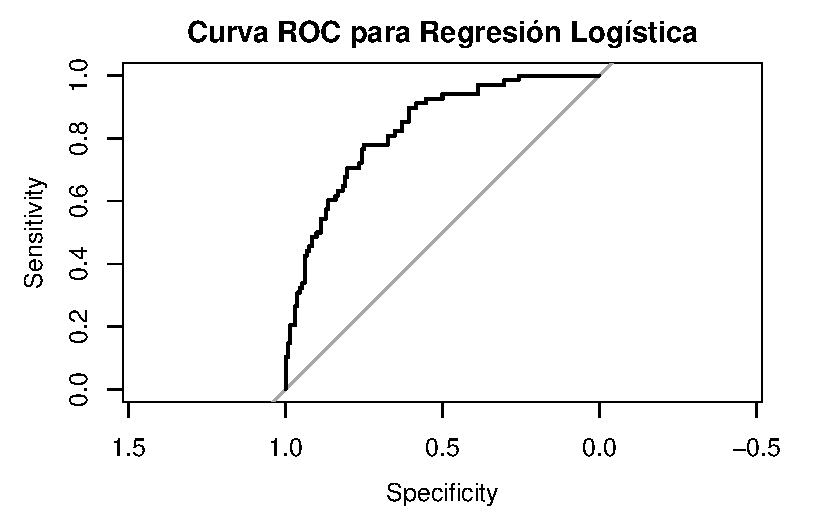
\includegraphics[keepaspectratio]{tema5_files/figure-pdf/log1-1.pdf}}

\begin{Shaded}
\begin{Highlighting}[]
\CommentTok{\# Calcular AUC}
\NormalTok{auc\_valor }\OtherTok{\textless{}{-}} \FunctionTok{auc}\NormalTok{(roc\_obj)}
\FunctionTok{print}\NormalTok{(}\FunctionTok{paste}\NormalTok{(}\StringTok{"AUC:"}\NormalTok{, }\FunctionTok{round}\NormalTok{(auc\_valor, }\DecValTok{3}\NormalTok{)))}
\end{Highlighting}
\end{Shaded}

\begin{verbatim}
[1] "AUC: 0.831"
\end{verbatim}

\end{tcolorbox}

\section{Regresión de Poisson}\label{regresiuxf3n-de-poisson}

La \textbf{regresión de Poisson} es una técnica estadística utilizada
para modelar \textbf{datos de conteo}, es decir, situaciones en las que
la variable dependiente representa el número de veces que ocurre un
evento en un período de tiempo o espacio específico (Coxe, West, and
Aiken 2009). Este tipo de modelo es adecuado cuando la variable
dependiente toma valores enteros no negativos (\(0, 1, 2, \dots\)) y
sigue una distribución de \textbf{Poisson}.

La distribución de Poisson describe la probabilidad de que ocurra un
número determinado de eventos en un intervalo fijo, dado que estos
eventos ocurren de forma independiente y a una tasa constante.

La \textbf{función de probabilidad} de la distribución de Poisson es:

\[
P(Y = y) = \frac{e^{-\lambda} \lambda^y}{y!}
\]

Donde:

\begin{itemize}
\tightlist
\item
  \(Y\) es la variable aleatoria que representa el número de eventos.
\item
  \(\lambda\) es la \textbf{tasa media de ocurrencia} de los eventos
  (esperanza de \(Y\)).
\item
  \(y\) es el número de eventos observados (\(y = 0, 1, 2, \dots\)).
\end{itemize}

\subsection{Modelo de regresión de
Poisson}\label{modelo-de-regresiuxf3n-de-poisson}

En la \textbf{regresión de Poisson}, el objetivo es modelar la relación
entre la \textbf{tasa de ocurrencia de los eventos} (\(\lambda\)) y un
conjunto de variables predictoras \(X_1, X_2, \dots, X_p\).

La \textbf{forma funcional} del modelo de Poisson es:

\[
\log(\lambda) = \beta_0 + \beta_1 X_1 + \beta_2 X_2 + \dots + \beta_p X_p
\]

Donde:

\begin{itemize}
\tightlist
\item
  \(\log(\lambda)\) es la \textbf{función de enlace logarítmica} que
  asegura que la tasa \(\lambda\) sea siempre positiva.
\item
  \(\beta_0, \beta_1, \dots, \beta_p\) son los coeficientes del modelo
  que describen la influencia de cada predictor sobre la tasa de
  eventos.
\end{itemize}

El modelo puede expresarse en términos de la \textbf{tasa esperada de
eventos} como:

\[
\lambda = e^{\beta_0 + \beta_1 X_1 + \beta_2 X_2 + \dots + \beta_p X_p}
\]

\subsection{Supuestos y limitaciones de la regresión de
Poisson}\label{supuestos-y-limitaciones-de-la-regresiuxf3n-de-poisson}

Tal y como ocurre en el modelo de regresión lineal, para que la
regresión de Poisson sea adecuada, se deben cumplir ciertos
\textbf{supuestos}:

\begin{itemize}
\item
  \textbf{Independencia de los eventos:} Los eventos deben ocurrir de
  manera independiente unos de otros.
\item
  \textbf{Distribución de Poisson de la variable dependiente:} La
  variable de respuesta debe seguir una distribución de Poisson, donde
  la \textbf{media} y la \textbf{varianza} son iguales:
\end{itemize}

\[
   E(Y) = Var(Y) = \lambda
   \]

\begin{itemize}
\item
  \textbf{No sobredispersión:} Uno de los problemas comunes en los datos
  de conteo es la \textbf{sobredispersión}, que ocurre cuando la
  varianza de los datos es mayor que la media (\(Var(Y) > E(Y)\)). La
  presencia de sobredispersión indica que el modelo de Poisson puede no
  ser adecuado, y puede ser necesario considerar modelos alternativos
  como la \textbf{regresión binomial negativa}.
\item
  \textbf{No exceso de ceros:} Si hay demasiados ceros en los datos (por
  ejemplo, en el número de accidentes en diferentes localidades donde
  muchas tienen cero accidentes), puede ser necesario utilizar modelos
  de \textbf{Poisson inflados en ceros (ZIP)} (Lambert 1992).
\end{itemize}

\subsection{Interpretación de los
resultados}\label{interpretaciuxf3n-de-los-resultados}

La interpretación de los coeficientes en la regresión de Poisson difiere
de la regresión lineal debido al uso de la función de enlace
logarítmica.

Los coeficientes \(\beta\) representan el \textbf{logaritmo de la tasa}
de eventos asociados con un cambio en la variable independiente. Para
interpretar en términos de la tasa de ocurrencia, se utiliza el
\textbf{exponencial de los coeficientes}:

\[
  e^{\beta_i}
\]

Esto representa el \textbf{factor de cambio multiplicativo} en la tasa
de eventos por cada unidad adicional en la variable \(X_i\).

\begin{tcolorbox}[enhanced jigsaw, leftrule=.75mm, breakable, colbacktitle=quarto-callout-important-color!10!white, bottomrule=.15mm, colframe=quarto-callout-important-color-frame, toprule=.15mm, colback=white, coltitle=black, bottomtitle=1mm, left=2mm, title=\textcolor{quarto-callout-important-color}{\faExclamation}\hspace{0.5em}{Interpretando el coeficiente de Poisson: Incidence Rate Ratio (IRR)}, opacityback=0, arc=.35mm, opacitybacktitle=0.6, toptitle=1mm, titlerule=0mm, rightrule=.15mm]

En la regresión de Poisson, el coeficiente \(\beta_j\) está en la escala
logarítmica de la tasa. Para una interpretación práctica, lo
exponenciamos para obtener el \textbf{Incidence Rate Ratio (IRR)}:

\[
\text{IRR} = e^{\beta_j}
\]

El IRR es un \textbf{factor multiplicativo} que nos dice cuánto cambia
la tasa de eventos esperada por cada incremento de una unidad en el
predictor \(X_j\).

\begin{itemize}
\tightlist
\item
  \textbf{Si IRR \textgreater{} 1}: Un incremento en \(X_j\) se asocia
  con un \textbf{aumento} en la tasa de eventos. Un IRR de 1.25
  significa que por cada unidad que aumenta \(X_j\), la tasa de eventos
  esperada se multiplica por 1.25 (es decir, aumenta un 25\%).
\item
  \textbf{Si IRR \textless{} 1}: Un incremento en \(X_j\) se asocia con
  una \textbf{disminución} en la tasa de eventos. Un IRR de 0.80
  significa que por cada unidad que aumenta \(X_j\), la tasa de eventos
  esperada se multiplica por 0.80 (es decir, disminuye un 20\%).
\item
  \textbf{Si IRR = 1}: La variable \(X_j\) no tiene efecto sobre la tasa
  de eventos.
\end{itemize}

\end{tcolorbox}

\begin{tcolorbox}[enhanced jigsaw, leftrule=.75mm, breakable, colbacktitle=quarto-callout-tip-color!10!white, bottomrule=.15mm, colframe=quarto-callout-tip-color-frame, toprule=.15mm, colback=white, coltitle=black, bottomtitle=1mm, left=2mm, title=\textcolor{quarto-callout-tip-color}{\faLightbulb}\hspace{0.5em}{Ejemplo}, opacityback=0, arc=.35mm, opacitybacktitle=0.6, toptitle=1mm, titlerule=0mm, rightrule=.15mm]

Vamos a utilizar R para ajustar un modelo de regresión de Poisson.
Supongamos que tenemos datos sobre el \textbf{número de accidentes de
tráfico} en diferentes intersecciones de una ciudad, junto con variables
como el volumen de tráfico y la visibilidad.

\begin{Shaded}
\begin{Highlighting}[]
\CommentTok{\# Simulación de datos para el número de accidentes}
\FunctionTok{set.seed}\NormalTok{(}\DecValTok{456}\NormalTok{)  }\CommentTok{\# Seed diferente para evitar duplicación}
\NormalTok{n }\OtherTok{\textless{}{-}} \DecValTok{100}  \CommentTok{\# Número de observaciones}

\CommentTok{\# Variables predictoras}
\NormalTok{trafico\_nuevo }\OtherTok{\textless{}{-}} \FunctionTok{rnorm}\NormalTok{(n, }\AttributeTok{mean =} \DecValTok{1000}\NormalTok{, }\AttributeTok{sd =} \DecValTok{300}\NormalTok{)  }\CommentTok{\# Volumen de tráfico en vehículos por día}
\NormalTok{visibilidad\_nueva }\OtherTok{\textless{}{-}} \FunctionTok{rnorm}\NormalTok{(n, }\AttributeTok{mean =} \DecValTok{5}\NormalTok{, }\AttributeTok{sd =} \DecValTok{2}\NormalTok{)   }\CommentTok{\# Visibilidad en kilómetros}

\CommentTok{\# Generar la tasa de accidentes (lambda) usando un modelo logarítmico}
\NormalTok{lambda\_nuevo }\OtherTok{\textless{}{-}} \FunctionTok{exp}\NormalTok{(}\FloatTok{0.01} \SpecialCharTok{*}\NormalTok{ trafico\_nuevo }\SpecialCharTok{{-}} \FloatTok{0.2} \SpecialCharTok{*}\NormalTok{ visibilidad\_nueva)}

\CommentTok{\# Generar el número de accidentes como una variable de Poisson}
\NormalTok{accidentes\_nuevo }\OtherTok{\textless{}{-}} \FunctionTok{rpois}\NormalTok{(n, }\AttributeTok{lambda =}\NormalTok{ lambda\_nuevo)}

\CommentTok{\# Crear el data frame}
\NormalTok{datos\_ejemplo }\OtherTok{\textless{}{-}} \FunctionTok{data.frame}\NormalTok{(}\AttributeTok{accidentes =}\NormalTok{ accidentes\_nuevo, }\AttributeTok{trafico =}\NormalTok{ trafico\_nuevo, }\AttributeTok{visibilidad =}\NormalTok{ visibilidad\_nueva)}
\FunctionTok{head}\NormalTok{(datos\_ejemplo)}
\end{Highlighting}
\end{Shaded}

\begin{verbatim}
  accidentes   trafico visibilidad
1        140  596.9436    5.236303
2      37153 1186.5327    6.739805
3      92909 1240.2624    4.816128
4        117  583.3323    5.137798
5       1793  785.6929    1.635146
6       1935  902.7817    7.233911
\end{verbatim}

\begin{Shaded}
\begin{Highlighting}[]
\CommentTok{\# Ajustar el modelo de regresión de Poisson}
\NormalTok{modelo\_ejemplo }\OtherTok{\textless{}{-}} \FunctionTok{glm}\NormalTok{(accidentes }\SpecialCharTok{\textasciitilde{}}\NormalTok{ trafico }\SpecialCharTok{+}\NormalTok{ visibilidad, }\AttributeTok{data =}\NormalTok{ datos\_ejemplo, }\AttributeTok{family =}\NormalTok{ poisson)}

\CommentTok{\# Resumen del modelo}
\FunctionTok{summary}\NormalTok{(modelo\_ejemplo)}
\end{Highlighting}
\end{Shaded}

\begin{verbatim}

Call:
glm(formula = accidentes ~ trafico + visibilidad, family = poisson, 
    data = datos_ejemplo)

Coefficients:
              Estimate Std. Error   z value Pr(>|z|)    
(Intercept)  9.607e-04  2.316e-03     0.415    0.678    
trafico      9.999e-03  1.360e-06  7350.127   <2e-16 ***
visibilidad -2.000e-01  1.012e-04 -1976.897   <2e-16 ***
---
Signif. codes:  0 '***' 0.001 '**' 0.01 '*' 0.05 '.' 0.1 ' ' 1

(Dispersion parameter for poisson family taken to be 1)

    Null deviance: 1.6856e+08  on 99  degrees of freedom
Residual deviance: 8.9300e+01  on 97  degrees of freedom
AIC: 1220.4

Number of Fisher Scoring iterations: 3
\end{verbatim}

El coeficiente asociado a \texttt{trafico} indica cómo el volumen de
tráfico afecta la tasa de accidentes.

El coeficiente asociado a \texttt{visibilidad} muestra cómo la
visibilidad afecta la frecuencia de accidentes.

\end{tcolorbox}

\subsection{Estimación por máxima verosimilitud en regresión de
Poisson}\label{estimaciuxf3n-por-muxe1xima-verosimilitud-en-regresiuxf3n-de-poisson}

La estimación de parámetros en regresión de Poisson utiliza también el
método de máxima verosimilitud, pero adaptado específicamente para la
distribución de Poisson con función de enlace logarítmica. Este enfoque
garantiza que las estimaciones aprovechen de manera óptima la
información contenida en los datos de conteo.

Para una muestra de \(n\) observaciones independientes, donde \(y_i\)
representa el conteo de eventos para la observación \(i\), la
\textbf{función de verosimilitud} se define como:

\[L(\boldsymbol{\beta}) = \prod_{i=1}^{n} \frac{e^{-\lambda_i} \lambda_i^{y_i}}{y_i!}\]

donde \(\lambda_i = e^{\mathbf{x}_i^T\boldsymbol{\beta}}\) es la tasa
esperada para la observación \(i\).

La \textbf{log-verosimilitud} correspondiente es:

\[\ell(\boldsymbol{\beta}) = \sum_{i=1}^{n} \left[y_i \log(\lambda_i) - \lambda_i - \log(y_i!)\right]\]

Sustituyendo \(\lambda_i = e^{\mathbf{x}_i^T\boldsymbol{\beta}}\):

\[\ell(\boldsymbol{\beta}) = \sum_{i=1}^{n} \left[y_i \mathbf{x}_i^T\boldsymbol{\beta} - e^{\mathbf{x}_i^T\boldsymbol{\beta}} - \log(y_i!)\right]\]

Para encontrar los valores de \(\boldsymbol{\beta}\) que maximizan la
log-verosimilitud, derivamos respecto a cada parámetro:

\[\frac{\partial \ell}{\partial \beta_j} = \sum_{i=1}^{n} x_{ij}(y_i - \lambda_i) = 0\]

Esta ecuación indica que los estimadores de máxima verosimilitud se
obtienen cuando la suma de los residuos (observado menos esperado)
ponderados por cada variable predictora es cero.

\subsubsection{Implementación del algoritmo
IRLS}\label{implementaciuxf3n-del-algoritmo-irls-1}

Dado que las ecuaciones de verosimilitud no tienen solución analítica
cerrada, se utiliza el algoritmo IRLS adaptado para regresión de
Poisson. Los elementos específicos son:

\textbf{Pesos:} \[w_i = \lambda_i\]

\textbf{Variable dependiente ajustada:}
\[z_i = \log(\lambda_i^{(t)}) + \frac{y_i - \lambda_i^{(t)}}{\lambda_i^{(t)}}\]

\textbf{Actualización de parámetros:}
\[\boldsymbol{\beta}^{(t+1)} = (\mathbf{X}^T \mathbf{W}^{(t)} \mathbf{X})^{-1} \mathbf{X}^T \mathbf{W}^{(t)} \mathbf{z}^{(t)}\]

\subsubsection{Propiedades específicas de la estimación
Poisson}\label{propiedades-especuxedficas-de-la-estimaciuxf3n-poisson}

La estimación por máxima verosimilitud en regresión de Poisson tiene
características particulares que la distinguen de otros GLMs:

\begin{enumerate}
\def\labelenumi{\arabic{enumi}.}
\item
  \textbf{Equidispersión}: El modelo asume que
  \(E(Y_i) = \text{Var}(Y_i) = \lambda_i\), lo que significa que la
  varianza aumenta linealmente con la media.
\item
  \textbf{Convergencia}: Generalmente requiere menos iteraciones que la
  regresión logística debido a la naturaleza más estable de la función
  de enlace logarítmica.
\item
  \textbf{Estabilidad numérica}: La función de enlace logarítmica
  garantiza automáticamente que \(\lambda_i > 0\), evitando problemas de
  valores negativos en las tasas estimadas.
\item
  \textbf{Interpretación multiplicativa}: Los coeficientes se
  interpretan como efectos multiplicativos sobre la tasa, lo que es
  natural para datos de conteo.
\end{enumerate}

\begin{tcolorbox}[enhanced jigsaw, leftrule=.75mm, breakable, colbacktitle=quarto-callout-tip-color!10!white, bottomrule=.15mm, colframe=quarto-callout-tip-color-frame, toprule=.15mm, colback=white, coltitle=black, bottomtitle=1mm, left=2mm, title=\textcolor{quarto-callout-tip-color}{\faLightbulb}\hspace{0.5em}{Ejemplo: Estimación paso a paso en regresión de Poisson}, opacityback=0, arc=.35mm, opacitybacktitle=0.6, toptitle=1mm, titlerule=0mm, rightrule=.15mm]

\begin{Shaded}
\begin{Highlighting}[]
\CommentTok{\# Demostración del proceso de estimación por máxima verosimilitud}
\CommentTok{\# Usar los datos simulados anteriores}
\FunctionTok{set.seed}\NormalTok{(}\DecValTok{123}\NormalTok{)}
\NormalTok{n }\OtherTok{\textless{}{-}} \DecValTok{100}
\NormalTok{trafico }\OtherTok{\textless{}{-}} \FunctionTok{rnorm}\NormalTok{(n, }\AttributeTok{mean =} \DecValTok{1000}\NormalTok{, }\AttributeTok{sd =} \DecValTok{300}\NormalTok{)}
\NormalTok{visibilidad }\OtherTok{\textless{}{-}} \FunctionTok{rnorm}\NormalTok{(n, }\AttributeTok{mean =} \DecValTok{5}\NormalTok{, }\AttributeTok{sd =} \DecValTok{2}\NormalTok{)}
\NormalTok{lambda }\OtherTok{\textless{}{-}} \FunctionTok{exp}\NormalTok{(}\SpecialCharTok{{-}}\DecValTok{2} \SpecialCharTok{+} \FloatTok{0.001}\SpecialCharTok{*}\NormalTok{trafico }\SpecialCharTok{{-}} \FloatTok{0.2}\SpecialCharTok{*}\NormalTok{visibilidad)}
\NormalTok{accidentes }\OtherTok{\textless{}{-}} \FunctionTok{rpois}\NormalTok{(n, lambda)}
\NormalTok{datos\_accidentes }\OtherTok{\textless{}{-}} \FunctionTok{data.frame}\NormalTok{(accidentes, trafico, visibilidad)}

\CommentTok{\# Función para calcular log{-}verosimilitud manualmente}
\NormalTok{log\_likelihood\_poisson }\OtherTok{\textless{}{-}} \ControlFlowTok{function}\NormalTok{(beta, X, y) \{}
\NormalTok{  eta }\OtherTok{\textless{}{-}}\NormalTok{ X }\SpecialCharTok{\%*\%}\NormalTok{ beta}
\NormalTok{  lambda }\OtherTok{\textless{}{-}} \FunctionTok{exp}\NormalTok{(eta)}
  \FunctionTok{sum}\NormalTok{(y }\SpecialCharTok{*} \FunctionTok{log}\NormalTok{(lambda) }\SpecialCharTok{{-}}\NormalTok{ lambda }\SpecialCharTok{{-}} \FunctionTok{lgamma}\NormalTok{(y }\SpecialCharTok{+} \DecValTok{1}\NormalTok{))}
\NormalTok{\}}

\CommentTok{\# Preparar datos}
\NormalTok{X }\OtherTok{\textless{}{-}} \FunctionTok{model.matrix}\NormalTok{(accidentes }\SpecialCharTok{\textasciitilde{}}\NormalTok{ trafico }\SpecialCharTok{+}\NormalTok{ visibilidad, }\AttributeTok{data =}\NormalTok{ datos\_accidentes)}
\NormalTok{y }\OtherTok{\textless{}{-}}\NormalTok{ datos\_accidentes}\SpecialCharTok{$}\NormalTok{accidentes}

\CommentTok{\# Ajuste con glm}
\NormalTok{modelo\_glm\_pois }\OtherTok{\textless{}{-}} \FunctionTok{glm}\NormalTok{(accidentes }\SpecialCharTok{\textasciitilde{}}\NormalTok{ trafico }\SpecialCharTok{+}\NormalTok{ visibilidad, }
                       \AttributeTok{data =}\NormalTok{ datos\_accidentes, }\AttributeTok{family =}\NormalTok{ poisson)}
\NormalTok{beta\_glm\_pois }\OtherTok{\textless{}{-}} \FunctionTok{coef}\NormalTok{(modelo\_glm\_pois)}

\FunctionTok{cat}\NormalTok{(}\StringTok{"=== ESTIMACIÓN POR MÁXIMA VEROSIMILITUD {-} POISSON ===}\SpecialCharTok{\textbackslash{}n}\StringTok{"}\NormalTok{)}
\end{Highlighting}
\end{Shaded}

\begin{verbatim}
=== ESTIMACIÓN POR MÁXIMA VEROSIMILITUD - POISSON ===
\end{verbatim}

\begin{Shaded}
\begin{Highlighting}[]
\FunctionTok{cat}\NormalTok{(}\StringTok{"Coeficientes estimados por glm():}\SpecialCharTok{\textbackslash{}n}\StringTok{"}\NormalTok{)}
\end{Highlighting}
\end{Shaded}

\begin{verbatim}
Coeficientes estimados por glm():
\end{verbatim}

\begin{Shaded}
\begin{Highlighting}[]
\FunctionTok{print}\NormalTok{(beta\_glm\_pois)}
\end{Highlighting}
\end{Shaded}

\begin{verbatim}
(Intercept)     trafico visibilidad 
-5.75588458  0.00284373  0.13082078 
\end{verbatim}

\begin{Shaded}
\begin{Highlighting}[]
\CommentTok{\# Verificar optimización}
\NormalTok{ll\_optimo\_pois }\OtherTok{\textless{}{-}} \FunctionTok{log\_likelihood\_poisson}\NormalTok{(beta\_glm\_pois, X, y)}
\FunctionTok{cat}\NormalTok{(}\StringTok{"}\SpecialCharTok{\textbackslash{}n}\StringTok{Log{-}verosimilitud en el óptimo:"}\NormalTok{, }\FunctionTok{round}\NormalTok{(ll\_optimo\_pois, }\DecValTok{4}\NormalTok{), }\StringTok{"}\SpecialCharTok{\textbackslash{}n}\StringTok{"}\NormalTok{)}
\end{Highlighting}
\end{Shaded}

\begin{verbatim}

Log-verosimilitud en el óptimo: -39.65 
\end{verbatim}

\begin{Shaded}
\begin{Highlighting}[]
\CommentTok{\# Interpretación multiplicativa}
\FunctionTok{cat}\NormalTok{(}\StringTok{"}\SpecialCharTok{\textbackslash{}n}\StringTok{Interpretación multiplicativa (exp(coeficientes)):}\SpecialCharTok{\textbackslash{}n}\StringTok{"}\NormalTok{)}
\end{Highlighting}
\end{Shaded}

\begin{verbatim}

Interpretación multiplicativa (exp(coeficientes)):
\end{verbatim}

\begin{Shaded}
\begin{Highlighting}[]
\NormalTok{exp\_coefs }\OtherTok{\textless{}{-}} \FunctionTok{exp}\NormalTok{(beta\_glm\_pois)}
\FunctionTok{print}\NormalTok{(exp\_coefs)}
\end{Highlighting}
\end{Shaded}

\begin{verbatim}
(Intercept)     trafico visibilidad 
0.003164106 1.002847777 1.139763495 
\end{verbatim}

\begin{Shaded}
\begin{Highlighting}[]
\FunctionTok{cat}\NormalTok{(}\StringTok{"}\SpecialCharTok{\textbackslash{}n}\StringTok{Interpretación:}\SpecialCharTok{\textbackslash{}n}\StringTok{"}\NormalTok{)}
\end{Highlighting}
\end{Shaded}

\begin{verbatim}

Interpretación:
\end{verbatim}

\begin{Shaded}
\begin{Highlighting}[]
\FunctionTok{cat}\NormalTok{(}\StringTok{"{-} Intercepto: Tasa base ="}\NormalTok{, }\FunctionTok{round}\NormalTok{(exp\_coefs[}\DecValTok{1}\NormalTok{], }\DecValTok{4}\NormalTok{), }\StringTok{"accidentes}\SpecialCharTok{\textbackslash{}n}\StringTok{"}\NormalTok{)}
\end{Highlighting}
\end{Shaded}

\begin{verbatim}
- Intercepto: Tasa base = 0.0032 accidentes
\end{verbatim}

\begin{Shaded}
\begin{Highlighting}[]
\FunctionTok{cat}\NormalTok{(}\StringTok{"{-} Tráfico: Por cada vehículo adicional, la tasa se multiplica por"}\NormalTok{, }\FunctionTok{round}\NormalTok{(exp\_coefs[}\DecValTok{2}\NormalTok{], }\DecValTok{6}\NormalTok{), }\StringTok{"}\SpecialCharTok{\textbackslash{}n}\StringTok{"}\NormalTok{)}
\end{Highlighting}
\end{Shaded}

\begin{verbatim}
- Tráfico: Por cada vehículo adicional, la tasa se multiplica por 1.002848 
\end{verbatim}

\begin{Shaded}
\begin{Highlighting}[]
\FunctionTok{cat}\NormalTok{(}\StringTok{"{-} Visibilidad: Por cada km adicional de visibilidad, la tasa se multiplica por"}\NormalTok{, }\FunctionTok{round}\NormalTok{(exp\_coefs[}\DecValTok{3}\NormalTok{], }\DecValTok{4}\NormalTok{), }\StringTok{"}\SpecialCharTok{\textbackslash{}n}\StringTok{"}\NormalTok{)}
\end{Highlighting}
\end{Shaded}

\begin{verbatim}
- Visibilidad: Por cada km adicional de visibilidad, la tasa se multiplica por 1.1398 
\end{verbatim}

\begin{Shaded}
\begin{Highlighting}[]
\CommentTok{\# Información de convergencia}
\FunctionTok{cat}\NormalTok{(}\StringTok{"}\SpecialCharTok{\textbackslash{}n}\StringTok{Información del algoritmo IRLS:}\SpecialCharTok{\textbackslash{}n}\StringTok{"}\NormalTok{)}
\end{Highlighting}
\end{Shaded}

\begin{verbatim}

Información del algoritmo IRLS:
\end{verbatim}

\begin{Shaded}
\begin{Highlighting}[]
\FunctionTok{cat}\NormalTok{(}\StringTok{"Iteraciones necesarias:"}\NormalTok{, modelo\_glm\_pois}\SpecialCharTok{$}\NormalTok{iter, }\StringTok{"}\SpecialCharTok{\textbackslash{}n}\StringTok{"}\NormalTok{)}
\end{Highlighting}
\end{Shaded}

\begin{verbatim}
Iteraciones necesarias: 6 
\end{verbatim}

\begin{Shaded}
\begin{Highlighting}[]
\FunctionTok{cat}\NormalTok{(}\StringTok{"¿Convergió?"}\NormalTok{, modelo\_glm\_pois}\SpecialCharTok{$}\NormalTok{converged, }\StringTok{"}\SpecialCharTok{\textbackslash{}n}\StringTok{"}\NormalTok{)}
\end{Highlighting}
\end{Shaded}

\begin{verbatim}
¿Convergió? TRUE 
\end{verbatim}

\begin{Shaded}
\begin{Highlighting}[]
\CommentTok{\# Verificar supuesto de equidispersión}
\NormalTok{media\_y }\OtherTok{\textless{}{-}} \FunctionTok{mean}\NormalTok{(y)}
\NormalTok{var\_y }\OtherTok{\textless{}{-}} \FunctionTok{var}\NormalTok{(y)}
\FunctionTok{cat}\NormalTok{(}\StringTok{"}\SpecialCharTok{\textbackslash{}n}\StringTok{Verificación de equidispersión:}\SpecialCharTok{\textbackslash{}n}\StringTok{"}\NormalTok{)}
\end{Highlighting}
\end{Shaded}

\begin{verbatim}

Verificación de equidispersión:
\end{verbatim}

\begin{Shaded}
\begin{Highlighting}[]
\FunctionTok{cat}\NormalTok{(}\StringTok{"Media observada:"}\NormalTok{, }\FunctionTok{round}\NormalTok{(media\_y, }\DecValTok{3}\NormalTok{), }\StringTok{"}\SpecialCharTok{\textbackslash{}n}\StringTok{"}\NormalTok{)}
\end{Highlighting}
\end{Shaded}

\begin{verbatim}
Media observada: 0.15 
\end{verbatim}

\begin{Shaded}
\begin{Highlighting}[]
\FunctionTok{cat}\NormalTok{(}\StringTok{"Varianza observada:"}\NormalTok{, }\FunctionTok{round}\NormalTok{(var\_y, }\DecValTok{3}\NormalTok{), }\StringTok{"}\SpecialCharTok{\textbackslash{}n}\StringTok{"}\NormalTok{)}
\end{Highlighting}
\end{Shaded}

\begin{verbatim}
Varianza observada: 0.149 
\end{verbatim}

\begin{Shaded}
\begin{Highlighting}[]
\FunctionTok{cat}\NormalTok{(}\StringTok{"Razón varianza/media:"}\NormalTok{, }\FunctionTok{round}\NormalTok{(var\_y}\SpecialCharTok{/}\NormalTok{media\_y, }\DecValTok{3}\NormalTok{), }\StringTok{"}\SpecialCharTok{\textbackslash{}n}\StringTok{"}\NormalTok{)}
\end{Highlighting}
\end{Shaded}

\begin{verbatim}
Razón varianza/media: 0.993 
\end{verbatim}

\end{tcolorbox}

\subsection{Bondad de ajuste en la regresión de
Poisson}\label{bondad-de-ajuste-en-la-regresiuxf3n-de-poisson}

Al igual que en la regresión logística, la bondad de ajuste en los
modelos de Poisson se aleja del \(R^2\) tradicional y se centra en
medidas basadas en la verosimilitud. El objetivo es cuantificar si el
modelo captura adecuadamente la estructura de los datos de conteo.

La \textbf{deviance} sigue siendo la métrica fundamental. Para la
regresión de Poisson, se calcula comparando la log-verosimilitud del
modelo ajustado con la de un modelo saturado (donde
\(\hat{\mu}_i = y_i\)). La fórmula específica es:
\[D = 2 \sum_{i=1}^{n} \left[ y_i \log\left(\frac{y_i}{\hat{\mu}_i}\right) - (y_i - \hat{\mu}_i) \right]\]
Donde el término \(y_i \log(y_i)\) se considera cero si \(y_i = 0\). Al
igual que en otros GLMs, la deviance es clave para comparar modelos
anidados mediante el \textbf{Test de la Razón de Verosimilitudes (LRT)}.

Sin embargo, para los modelos de Poisson, la prueba de bondad de ajuste
más importante en la práctica es la evaluación de la
\textbf{sobredispersión}. Un buen ajuste del modelo de Poisson implica
que se cumple el supuesto de equidispersión (\(Var(Y) = \mu\)). Por lo
tanto, el \textbf{estadístico de dispersión} (\(\hat{\phi}\)) se
convierte en una medida de facto de la bondad de ajuste:
\[\hat{\phi} = \frac{X^2_{\text{Pearson}}}{n-p}\] Un valor de
\(\hat{\phi}\) cercano a 1 indica que el supuesto de la distribución de
Poisson se cumple y que el ajuste del modelo es adecuado. Si
\(\hat{\phi}\) es significativamente mayor que 1, el modelo no se ajusta
bien a la variabilidad de los datos, y este es el principal indicador
para buscar alternativas como la regresión binomial negativa.

Aunque los \textbf{pseudo R²} (como el de McFadden) pueden calcularse,
son menos utilizados e informativos en el contexto de la regresión de
Poisson en comparación con el análisis de la dispersión.

\subsection{Validación del modelo de
Poisson}\label{validaciuxf3n-del-modelo-de-poisson}

A diferencia de la regresión logística, donde la validación se centra en
la capacidad de \emph{clasificación}, la validación de un modelo de
Poisson se enfoca en su \textbf{capacidad de predicción}: ¿qué tan cerca
están los conteos predichos por el modelo de los conteos reales
observados?

El proceso de validación suele implicar la división de los datos en un
conjunto de \textbf{entrenamiento (train)} y uno de \textbf{prueba
(test)}. El modelo se ajusta con los datos de entrenamiento y su
rendimiento predictivo se evalúa sobre los datos de prueba, que el
modelo no ha visto antes. Esto nos da una estimación honesta de cómo
generalizará el modelo a nuevos datos.

Las métricas de validación principales para modelos de conteo son:

\begin{itemize}
\item
  \textbf{Raíz del Error Cuadrático Medio (RMSE):} Es una de las
  métricas más comunes y mide la desviación estándar de los residuos.
  Penaliza más los errores grandes. \[
  \text{RMSE} = \sqrt{\frac{1}{n}\sum_{i=1}^{n}(y_i - \hat{\mu}_i)^2}
  \]
\item
  \textbf{Error Absoluto Medio (MAE):} Mide la magnitud promedio de los
  errores, siendo menos sensible a valores atípicos que el RMSE. \[
  \text{MAE} = \frac{1}{n}\sum_{i=1}^{n}|y_i - \hat{\mu}_i|
  \]
\end{itemize}

Ambas métricas se expresan en las mismas unidades que la variable de
respuesta (por ejemplo, ``accidentes'', ``compras''), lo que facilita su
interpretación. Un modelo con valores de RMSE y MAE más bajos en el
conjunto de prueba se considera que tiene un mejor rendimiento
predictivo.

Una herramienta visual clave para la validación es el \textbf{gráfico de
valores predichos vs.~valores reales} en el conjunto de prueba. En un
modelo con buena capacidad predictiva, los puntos deberían agruparse
cerca de la línea diagonal \(y=x\), indicando que las predicciones
(\(\hat{\mu}_i\)) son cercanas a los valores observados (\(y_i\)).

\section{Otros GLMs}\label{otros-glms}

La \textbf{regresión binomial negativa} y los \textbf{modelos basados en
distribuciones como Gamma e Inversa Gaussiana} amplían la capacidad de
los \textbf{Modelos Lineales Generalizados (GLM)} para adaptarse a una
amplia variedad de situaciones del mundo real. Estos modelos son
especialmente útiles cuando los datos presentan características como
sobredispersión, sesgo o restricciones en el dominio (por ejemplo, solo
valores positivos). La elección adecuada del modelo y la función de
enlace garantiza predicciones precisas y válidas, contribuyendo a la
toma de decisiones informadas en campos como la salud, la ingeniería y
la economía.

\subsection{Regresión binomial
negativa}\label{regresiuxf3n-binomial-negativa}

Tal y como hemos visto en apartados anteriores, la
\textbf{sobredispersión} ocurre cuando la varianza de los datos de
conteo es \textbf{mayor que la media}, lo cual viola uno de los
supuestos clave de la regresión de Poisson, que asume que la media y la
varianza son iguales (\(E(Y) = Var(Y) = \lambda\)). La sobredispersión
puede surgir por varias razones:

\begin{itemize}
\tightlist
\item
  \textbf{Heterogeneidad no modelada:} Existen factores que afectan la
  variable dependiente pero no han sido incluidos en el modelo.
\item
  \textbf{Dependencia entre eventos:} Los eventos no ocurren de forma
  independiente.
\item
  \textbf{Exceso de ceros:} Hay más ceros en los datos de los que
  predice la distribución de Poisson.
\end{itemize}

Cuando la sobredispersión está presente, la regresión de Poisson
subestima los errores estándar, lo que puede llevar a conclusiones
incorrectas sobre la significancia de los predictores.

La \textbf{regresión binomial negativa} es una extensión de la regresión
de Poisson que introduce un parámetro adicional para manejar la
sobredispersión. Este modelo permite que la varianza sea mayor que la
media:

\[
Var(Y) = \lambda + \alpha \lambda^2
\]

Donde \(\alpha\) es el parámetro de dispersión. Si \(\alpha = 0\), el
modelo se reduce a la regresión de Poisson.

La forma funcional del modelo binomial negativo es similar al de
Poisson:

\[
\log(\lambda) = \beta_0 + \beta_1 X_1 + \beta_2 X_2 + \dots + \beta_p X_p
\]

Pero la varianza ahora incluye el término adicional \(\alpha\) para
capturar la sobredispersión.

\begin{tcolorbox}[enhanced jigsaw, leftrule=.75mm, breakable, colbacktitle=quarto-callout-tip-color!10!white, bottomrule=.15mm, colframe=quarto-callout-tip-color-frame, toprule=.15mm, colback=white, coltitle=black, bottomtitle=1mm, left=2mm, title=\textcolor{quarto-callout-tip-color}{\faLightbulb}\hspace{0.5em}{Ejemplo}, opacityback=0, arc=.35mm, opacitybacktitle=0.6, toptitle=1mm, titlerule=0mm, rightrule=.15mm]

\begin{Shaded}
\begin{Highlighting}[]
\CommentTok{\# Instalar y cargar la librería MASS que contiene la función glm.nb}
\FunctionTok{library}\NormalTok{(MASS)}

\CommentTok{\# Usar los datos de accidentes del ejemplo anterior}
\CommentTok{\# Ajuste de un modelo binomial negativo}
\NormalTok{modelo\_binom\_neg }\OtherTok{\textless{}{-}} \FunctionTok{glm.nb}\NormalTok{(accidentes }\SpecialCharTok{\textasciitilde{}}\NormalTok{ trafico }\SpecialCharTok{+}\NormalTok{ visibilidad, }\AttributeTok{data =}\NormalTok{ datos\_accidentes)}
\end{Highlighting}
\end{Shaded}

\begin{verbatim}
Warning in theta.ml(Y, mu, sum(w), w, limit = control$maxit, trace =
control$trace > : iteration limit reached
Warning in theta.ml(Y, mu, sum(w), w, limit = control$maxit, trace =
control$trace > : iteration limit reached
\end{verbatim}

\begin{Shaded}
\begin{Highlighting}[]
\CommentTok{\# Resumen del modelo}
\FunctionTok{summary}\NormalTok{(modelo\_binom\_neg)}
\end{Highlighting}
\end{Shaded}

\begin{verbatim}

Call:
glm.nb(formula = accidentes ~ trafico + visibilidad, data = datos_accidentes, 
    init.theta = 2158.536301, link = log)

Coefficients:
              Estimate Std. Error z value Pr(>|z|)    
(Intercept) -5.7560791  1.5223127  -3.781 0.000156 ***
trafico      0.0028439  0.0009831   2.893 0.003818 ** 
visibilidad  0.1308306  0.1402185   0.933 0.350795    
---
Signif. codes:  0 '***' 0.001 '**' 0.01 '*' 0.05 '.' 0.1 ' ' 1

(Dispersion parameter for Negative Binomial(2158.536) family taken to be 1)

    Null deviance: 59.679  on 99  degrees of freedom
Residual deviance: 50.680  on 97  degrees of freedom
AIC: 87.301

Number of Fisher Scoring iterations: 1

              Theta:  2159 
          Std. Err.:  49427 
Warning while fitting theta: iteration limit reached 

 2 x log-likelihood:  -79.301 
\end{verbatim}

\begin{Shaded}
\begin{Highlighting}[]
\CommentTok{\# Comparar la dispersión con el modelo de Poisson}
\FunctionTok{cat}\NormalTok{(}\StringTok{"Dispersión en Poisson (deviance/df.residual):"}\NormalTok{, }\FunctionTok{round}\NormalTok{(modelo\_glm\_pois}\SpecialCharTok{$}\NormalTok{deviance }\SpecialCharTok{/}\NormalTok{ modelo\_glm\_pois}\SpecialCharTok{$}\NormalTok{df.residual, }\DecValTok{3}\NormalTok{), }\StringTok{"}\SpecialCharTok{\textbackslash{}n}\StringTok{"}\NormalTok{)}
\end{Highlighting}
\end{Shaded}

\begin{verbatim}
Dispersión en Poisson (deviance/df.residual): 0.523 
\end{verbatim}

\begin{Shaded}
\begin{Highlighting}[]
\FunctionTok{cat}\NormalTok{(}\StringTok{"Parámetro theta en Binomial Negativa:"}\NormalTok{, }\FunctionTok{round}\NormalTok{(modelo\_binom\_neg}\SpecialCharTok{$}\NormalTok{theta, }\DecValTok{3}\NormalTok{), }\StringTok{"}\SpecialCharTok{\textbackslash{}n}\StringTok{"}\NormalTok{)}
\end{Highlighting}
\end{Shaded}

\begin{verbatim}
Parámetro theta en Binomial Negativa: 2158.536 
\end{verbatim}

\begin{Shaded}
\begin{Highlighting}[]
\CommentTok{\# Comparar AIC}
\FunctionTok{cat}\NormalTok{(}\StringTok{"AIC Poisson:"}\NormalTok{, }\FunctionTok{round}\NormalTok{(}\FunctionTok{AIC}\NormalTok{(modelo\_glm\_pois), }\DecValTok{2}\NormalTok{), }\StringTok{"}\SpecialCharTok{\textbackslash{}n}\StringTok{"}\NormalTok{)}
\end{Highlighting}
\end{Shaded}

\begin{verbatim}
AIC Poisson: 85.3 
\end{verbatim}

\begin{Shaded}
\begin{Highlighting}[]
\FunctionTok{cat}\NormalTok{(}\StringTok{"AIC Binomial Negativa:"}\NormalTok{, }\FunctionTok{round}\NormalTok{(}\FunctionTok{AIC}\NormalTok{(modelo\_binom\_neg), }\DecValTok{2}\NormalTok{), }\StringTok{"}\SpecialCharTok{\textbackslash{}n}\StringTok{"}\NormalTok{)}
\end{Highlighting}
\end{Shaded}

\begin{verbatim}
AIC Binomial Negativa: 87.3 
\end{verbatim}

\end{tcolorbox}

\textbf{Interpretación del parámetro \(\theta\) en binomial negativa:}

\begin{itemize}
\tightlist
\item
  El parámetro \(\theta\) controla el grado de sobredispersión en el
  modelo
\item
  \textbf{Valores altos de \(\theta\)} (ej: \(\theta > 100\)): Poca
  sobredispersión, el modelo se aproxima a Poisson
\item
  \textbf{Valores bajos de \(\theta\)} (ej: \(\theta < 10\)): Mucha
  sobredispersión, diferencia significativa respecto a Poisson
\item
  \textbf{Regla práctica}: Si \(\theta\) es pequeño, confirma que había
  sobredispersión y que el modelo binomial negativa es más apropiado que
  Poisson
\end{itemize}

\textbf{Comparación de modelos:} - Si AIC de binomial negativa
\textless{} AIC de Poisson → preferir binomial negativa - El modelo
binomial negativa corrige la subestimación de errores estándar que
ocurre en Poisson con sobredispersión

\subsection{Modelos para variables continuas no
normales}\label{modelos-para-variables-continuas-no-normales}

Existen situaciones en las que la variable dependiente es
\textbf{continua}, pero \textbf{no sigue una distribución normal}. En
estos casos, los \textbf{Modelos Lineales Generalizados (GLM)} permiten
utilizar distribuciones alternativas como \textbf{Gamma} o
\textbf{Inversa Gaussiana}, junto con funciones de enlace específicas.

\subsubsection{Regresión gamma para datos positivos y
sesgados}\label{regresiuxf3n-gamma-para-datos-positivos-y-sesgados}

La \textbf{regresión Gamma} es adecuada para modelar variables continuas
que son \textbf{positivas} y tienen una distribución \textbf{sesgada a
la derecha}. Ejemplos típicos incluyen tiempos de espera, costos médicos
o duración de procesos.

\begin{itemize}
\tightlist
\item
  La distribución Gamma asume que la variable dependiente es continua y
  positiva.
\item
  La varianza de la variable dependiente aumenta proporcionalmente al
  cuadrado de la media.
\end{itemize}

\textbf{Función de Enlace Común:}
\[\log(\mu) = \beta_0 + \beta_1 X_1 + \dots + \beta_p X_p\]

\begin{tcolorbox}[enhanced jigsaw, leftrule=.75mm, breakable, colbacktitle=quarto-callout-tip-color!10!white, bottomrule=.15mm, colframe=quarto-callout-tip-color-frame, toprule=.15mm, colback=white, coltitle=black, bottomtitle=1mm, left=2mm, title=\textcolor{quarto-callout-tip-color}{\faLightbulb}\hspace{0.5em}{Ejemplo}, opacityback=0, arc=.35mm, opacitybacktitle=0.6, toptitle=1mm, titlerule=0mm, rightrule=.15mm]

\begin{Shaded}
\begin{Highlighting}[]
\CommentTok{\# Simulación de costos médicos}
\FunctionTok{set.seed}\NormalTok{(}\DecValTok{123}\NormalTok{)}
\NormalTok{n }\OtherTok{\textless{}{-}} \DecValTok{100}
\NormalTok{ingresos }\OtherTok{\textless{}{-}} \FunctionTok{rnorm}\NormalTok{(n, }\AttributeTok{mean =} \DecValTok{50000}\NormalTok{, }\AttributeTok{sd =} \DecValTok{10000}\NormalTok{)}
\NormalTok{edad }\OtherTok{\textless{}{-}} \FunctionTok{rnorm}\NormalTok{(n, }\AttributeTok{mean =} \DecValTok{45}\NormalTok{, }\AttributeTok{sd =} \DecValTok{10}\NormalTok{)}
\NormalTok{costos }\OtherTok{\textless{}{-}} \FunctionTok{rgamma}\NormalTok{(n, }\AttributeTok{shape =} \DecValTok{2}\NormalTok{, }\AttributeTok{rate =} \FloatTok{0.00005} \SpecialCharTok{*}\NormalTok{ ingresos }\SpecialCharTok{+} \FloatTok{0.01} \SpecialCharTok{*}\NormalTok{ edad)}

\CommentTok{\# Ajuste del modelo Gamma}
\NormalTok{modelo\_gamma }\OtherTok{\textless{}{-}} \FunctionTok{glm}\NormalTok{(costos }\SpecialCharTok{\textasciitilde{}}\NormalTok{ ingresos }\SpecialCharTok{+}\NormalTok{ edad, }\AttributeTok{family =} \FunctionTok{Gamma}\NormalTok{(}\AttributeTok{link =} \StringTok{"log"}\NormalTok{))}

\CommentTok{\# Resumen del modelo}
\FunctionTok{summary}\NormalTok{(modelo\_gamma)}
\end{Highlighting}
\end{Shaded}

\begin{verbatim}

Call:
glm(formula = costos ~ ingresos + edad, family = Gamma(link = "log"))

Coefficients:
              Estimate Std. Error t value Pr(>|t|)  
(Intercept)  3.440e-01  5.294e-01   0.650   0.5173  
ingresos    -1.807e-05  7.804e-06  -2.316   0.0227 *
edad         3.584e-03  7.366e-03   0.487   0.6277  
---
Signif. codes:  0 '***' 0.001 '**' 0.01 '*' 0.05 '.' 0.1 ' ' 1

(Dispersion parameter for Gamma family taken to be 0.5010938)

    Null deviance: 60.771  on 99  degrees of freedom
Residual deviance: 58.345  on 97  degrees of freedom
AIC: 105.47

Number of Fisher Scoring iterations: 5
\end{verbatim}

\begin{itemize}
\tightlist
\item
  Los coeficientes muestran cómo los ingresos y la edad afectan los
  costos médicos esperados.
\item
  El enlace logarítmico asegura que las predicciones sean siempre
  positivas.
\end{itemize}

\end{tcolorbox}

\subsubsection{Regresión inversa
gaussiana}\label{regresiuxf3n-inversa-gaussiana}

La \textbf{regresión Inversa Gaussiana} es útil para modelar tiempos de
respuesta o variables donde la varianza disminuye rápidamente a medida
que la media aumenta. Este modelo se aplica en campos como la
ingeniería, donde se analizan tiempos hasta fallas de sistemas.

\textbf{Función de Enlace Común:}
\[\frac{1}{\mu^2} = \beta_0 + \beta_1 X_1 + \dots + \beta_p X_p\]

\begin{tcolorbox}[enhanced jigsaw, leftrule=.75mm, breakable, colbacktitle=quarto-callout-tip-color!10!white, bottomrule=.15mm, colframe=quarto-callout-tip-color-frame, toprule=.15mm, colback=white, coltitle=black, bottomtitle=1mm, left=2mm, title=\textcolor{quarto-callout-tip-color}{\faLightbulb}\hspace{0.5em}{Ejemplo}, opacityback=0, arc=.35mm, opacitybacktitle=0.6, toptitle=1mm, titlerule=0mm, rightrule=.15mm]

\begin{Shaded}
\begin{Highlighting}[]
\CommentTok{\# Instalar y cargar la librería correcta}
\FunctionTok{library}\NormalTok{(statmod)}

\CommentTok{\# Simulación de datos}
\FunctionTok{set.seed}\NormalTok{(}\DecValTok{123}\NormalTok{)}
\NormalTok{n }\OtherTok{\textless{}{-}} \DecValTok{100}
\NormalTok{carga\_trabajo }\OtherTok{\textless{}{-}} \FunctionTok{rnorm}\NormalTok{(n, }\AttributeTok{mean =} \DecValTok{50}\NormalTok{, }\AttributeTok{sd =} \DecValTok{10}\NormalTok{)}

\CommentTok{\# Generar tiempos hasta el fallo usando la distribución inversa gaussiana}
\CommentTok{\# Aseguramos que los valores de carga\_trabajo sean positivos para evitar problemas numéricos}
\NormalTok{carga\_trabajo[carga\_trabajo }\SpecialCharTok{\textless{}=} \DecValTok{0}\NormalTok{] }\OtherTok{\textless{}{-}} \DecValTok{1}
\NormalTok{tiempo\_fallo }\OtherTok{\textless{}{-}} \FunctionTok{rinvgauss}\NormalTok{(n, }\AttributeTok{mean =} \DecValTok{100} \SpecialCharTok{/}\NormalTok{ carga\_trabajo, }\AttributeTok{dispersion =} \DecValTok{1}\NormalTok{)}

\CommentTok{\# Ajuste del modelo Inversa Gaussiana con enlace logarítmico}
\NormalTok{modelo\_inversa\_gauss }\OtherTok{\textless{}{-}} \FunctionTok{glm}\NormalTok{(tiempo\_fallo }\SpecialCharTok{\textasciitilde{}}\NormalTok{ carga\_trabajo, }\AttributeTok{family =} \FunctionTok{inverse.gaussian}\NormalTok{(}\AttributeTok{link =} \StringTok{"1/mu\^{}2"}\NormalTok{),}\AttributeTok{start =} \FunctionTok{c}\NormalTok{(}\FloatTok{0.01}\NormalTok{, }\FloatTok{0.01}\NormalTok{))}
\end{Highlighting}
\end{Shaded}

\begin{verbatim}
Warning in sqrt(eta): NaNs produced
\end{verbatim}

\begin{verbatim}
Warning: step size truncated due to divergence
\end{verbatim}

\begin{Shaded}
\begin{Highlighting}[]
\CommentTok{\# Resumen del modelo}
\FunctionTok{summary}\NormalTok{(modelo\_inversa\_gauss)}
\end{Highlighting}
\end{Shaded}

\begin{verbatim}

Call:
glm(formula = tiempo_fallo ~ carga_trabajo, family = inverse.gaussian(link = "1/mu^2"), 
    start = c(0.01, 0.01))

Coefficients:
               Estimate Std. Error t value Pr(>|t|)
(Intercept)   -0.106143   0.462230  -0.230    0.819
carga_trabajo  0.008261   0.009623   0.859    0.393

(Dispersion parameter for inverse.gaussian family taken to be 1.348442)

    Null deviance: 94.085  on 99  degrees of freedom
Residual deviance: 93.171  on 98  degrees of freedom
AIC: 294.2

Number of Fisher Scoring iterations: 5
\end{verbatim}

\end{tcolorbox}

\begin{tcolorbox}[enhanced jigsaw, leftrule=.75mm, breakable, colbacktitle=quarto-callout-warning-color!10!white, bottomrule=.15mm, colframe=quarto-callout-warning-color-frame, toprule=.15mm, colback=white, coltitle=black, bottomtitle=1mm, left=2mm, title=\textcolor{quarto-callout-warning-color}{\faExclamationTriangle}\hspace{0.5em}{¿Qué GLM debo usar?}, opacityback=0, arc=.35mm, opacitybacktitle=0.6, toptitle=1mm, titlerule=0mm, rightrule=.15mm]

La elección del modelo correcto depende casi exclusivamente de la
naturaleza de tu variable respuesta (\(Y\)). Aquí tienes una guía
rápida:

\begin{itemize}
\tightlist
\item
  \textbf{¿Tu variable respuesta es binaria (Sí/No, 0/1,
  Éxito/Fracaso)?}

  \begin{itemize}
  \tightlist
  \item
    Usa \textbf{Regresión Logística}.
  \end{itemize}
\item
  \textbf{¿Tu variable respuesta es un conteo de eventos (nº de
  accidentes, nº de clientes, nº de fallos)?}

  \begin{itemize}
  \tightlist
  \item
    Empieza con una \textbf{Regresión de Poisson}.
  \item
    \textbf{Importante:} Después de ajustar el modelo, comprueba si hay
    \textbf{sobredispersión}.
  \item
    Si la hay (estadístico de dispersión \(\hat{\phi} > 1.5\) o la
    teoría lo sugiere), cambia a una \textbf{Regresión Binomial
    Negativa}.
  \end{itemize}
\item
  \textbf{¿Tu variable respuesta es continua y estrictamente positiva,
  con una distribución asimétrica hacia la derecha (ej. tiempos, costos,
  reclamaciones de seguros)?}

  \begin{itemize}
  \tightlist
  \item
    Usa \textbf{Regresión Gamma}. Es una excelente alternativa a
    transformar la variable con logaritmos y usar un modelo lineal.
  \end{itemize}
\item
  \textbf{¿Tu variable respuesta es un tiempo hasta un evento y tiene
  una asimetría muy pronunciada?}

  \begin{itemize}
  \tightlist
  \item
    Considera una \textbf{Regresión Inversa Gaussiana}.
  \end{itemize}
\end{itemize}

\end{tcolorbox}

\bookmarksetup{startatroot}

\chapter{Conclusiones}\label{sec-conclusiones}

A lo largo de seis capítulos hemos presentado el material de la
asignatura de \textbf{Modelos Estadísticos para la Predicción} del Grado
en \textbf{Matemáticas}.

En este capítulo final, te invitamos a reflexionar sobre las principales
lecciones aprendidas durante el curso y a destacar cómo el rigor
matemático que caracteriza vuestra formación se convierte en una
herramienta indispensable para dominar el modelado estadístico. Además,
animamos a los estudiantes a continuar explorando y ampliando sus
conocimientos en cursos posteriores, consolidando así una base sólida
para afrontar los desafíos de la ciencia de datos moderna desde una
perspectiva analítica y fundamentada.

Al finalizar este recorrido, queda patente que el modelado estadístico
es mucho más que una colección de técnicas; es un marco de pensamiento
estructurado para comprender la incertidumbre y extraer conocimiento a
partir de los datos. Hemos transitado desde los axiomas teóricos de la
regresión hasta su aplicación computacional, equipando a los futuros
matemáticos con las herramientas para construir, validar e interpretar
modelos robustos.

\section{Resumen de los aprendizajes}\label{resumen-de-los-aprendizajes}

A lo largo de este manual, hemos construido un conocimiento progresivo
sobre el modelado predictivo, cubriendo los siguientes pilares:

\begin{enumerate}
\def\labelenumi{\arabic{enumi}.}
\item
  \textbf{Fundamentos del modelado lineal: simple y múltiple}: Hemos
  partido de la formulación teórica del \textbf{modelo lineal},
  estableciendo sus componentes axiomáticos y los supuestos de
  Gauss-Markov que garantizan las propiedades óptimas de los estimadores
  de \textbf{Mínimos Cuadrados Ordinarios (MCO)}. Se ha hecho hincapié
  en la transición del modelo simple al múltiple, destacando el
  principio de \emph{ceteris paribus} para la interpretación de
  coeficientes, el diagnóstico de la \textbf{multicolinealidad} mediante
  el VIF y la evaluación de la bondad de ajuste a través de la
  descomposición ANOVA y el \(R^2\) ajustado.
\item
  \textbf{Ingeniería de características y flexibilidad del modelo}:
  Exploramos cómo superar las limitaciones de un modelo estrictamente
  lineal. Aprendimos a diagnosticar y corregir violaciones de los
  supuestos mediante \textbf{transformaciones de variables}
  (logarítmica, Box-Cox), a incorporar predictores no numéricos a través
  de la codificación de \textbf{variables categóricas}, y,
  fundamentalmente, a modelar relaciones complejas mediante la inclusión
  de \textbf{términos de interacción}, entendiendo cómo el efecto de un
  predictor puede depender del valor de otro.
\item
  \textbf{Selección de variables, regularización y validación}:
  Abordamos el crucial dilema sesgo-varianza y la necesidad de construir
  modelos parsimoniosos que generalicen bien a datos no observados. Se
  presentaron los \textbf{criterios de información (AIC, BIC)} y los
  \textbf{métodos por pasos (stepwise)} como herramientas para comparar
  y seleccionar modelos. Profundizamos en los métodos de
  \textbf{regularización (Ridge, Lasso y Elastic Net)}, que ofrecen una
  alternativa moderna y robusta para manejar la multicolinealidad y
  realizar selección de variables de forma simultánea, especialmente en
  contextos de alta dimensionalidad. Finalmente, se consolidó la
  importancia de la \textbf{validación cruzada} como el estándar para
  una evaluación honesta del rendimiento predictivo del modelo.
\item
  \textbf{Modelos lineales generalizados (GLM)}: Expandimos el marco de
  la regresión más allá de la asunción de normalidad en la variable
  respuesta. A través de la introducción de la \textbf{familia
  exponencial} de distribuciones y las \textbf{funciones de enlace},
  entendimos cómo adaptar el modelo lineal a diferentes tipos de datos.
  Nos centramos en dos de los GLM más importantes: la \textbf{Regresión
  Logística} para modelar resultados binarios y la \textbf{Regresión de
  Poisson} para datos de conteo, aprendiendo a interpretar sus
  coeficientes en términos de odds ratios y tasas de eventos,
  respectivamente.
\end{enumerate}

\section{Reflexiones finales}\label{reflexiones-finales}

El estudio de los \textbf{Modelos Estadísticos para la Predicción} dota
al matemático de un puente entre la teoría abstracta y la resolución de
problemas del mundo real. A lo largo de este curso, hemos visto cómo
conceptos rigurosos ---espacios vectoriales en la geometría de MCO,
optimización en la estimación de parámetros, y teoría de la probabilidad
en la inferencia--- se materializan en herramientas prácticas para la
toma de decisiones bajo incertidumbre.

Hemos aprendido que construir un modelo no es un acto mecánico, sino un
proceso iterativo de \textbf{diagnóstico, crítica y refinamiento}. La
capacidad para evaluar la validez de los supuestos, interpretar los
resultados con cautela y comunicar tanto las fortalezas como las
limitaciones de un modelo es lo que distingue a un analista competente.
La \textbf{interpretabilidad} y la \textbf{validación rigurosa} no son
meros pasos finales, sino el núcleo de una práctica estadística honesta
y efectiva.

En un mundo saturado de datos, la habilidad para construir modelos que
no solo predicen, sino que también explican y ofrecen certidumbre
cuantificable, es más valiosa que nunca.

\section{Proyección futura: El valor del rigor
matemático}\label{proyecciuxf3n-futura-el-valor-del-rigor-matemuxe1tico}

Las competencias adquiridas en esta asignatura son la culminación de
vuestra carrera, el punto donde el álgebra lineal, el cálculo y la
optimización se convierten en el motor de la modelización estadística
aplicada. Vuestra formación matemática os proporciona una ventaja
fundamental: la capacidad de ir más allá de la aplicación mecánica de un
algoritmo para comprender en profundidad los supuestos que lo sustentan,
la geometría de su funcionamiento y la incertidumbre inherente a sus
conclusiones.

Conceptos como la regularización y la validación cruzada son el lenguaje
compartido con el \textbf{Aprendizaje Automático}. Mientras que el
Aprendizaje Automático a menudo se centra en la potencia predictiva de
algoritmos complejos, este curso os ha proporcionado la ``gramática''
estadística para construir modelos interpretables, diagnosticar su
validez y cuantificar la fiabilidad de sus resultados. Esta base teórica
es indispensable para aplicar, y en un futuro desarrollar, cualquier
técnica de modelado de forma rigurosa y responsable.

Esta habilidad para analizar críticamente los modelos es precisamente lo
que el mercado y el mundo académico demandan. Os posiciona de manera
ideal para roles avanzados como \textbf{Científico de Datos},
\textbf{Analista Cuantitativo (`Quant')} en el sector financiero, o
\textbf{Bioestadístico}, así como para continuar vuestra formación con
\textbf{estudios de postgrado (Máster o Doctorado)} donde la
investigación y el desarrollo de nuevos métodos es primordial.

En definitiva, habéis adquirido un conjunto de herramientas analíticas
que os permitirá traducir problemas complejos en modelos manejables y
basados en evidencia.

¡Mucha suerte en vuestra trayectoria profesional!

\bookmarksetup{startatroot}

\chapter*{Bibliografía}\label{bibliografuxeda}
\addcontentsline{toc}{chapter}{Bibliografía}

\markboth{Bibliografía}{Bibliografía}

\phantomsection\label{refs}
\begin{CSLReferences}{1}{0}
\bibitem[\citeproctext]{ref-bates2015}
Bates, Douglas, Martin Mächler, Ben Bolker, and Steve Walker. 2015.
{``Fitting Linear Mixed-Effects Models Using Lme4.''} \emph{Journal of
Statistical Software} 67 (1): 1--48.

\bibitem[\citeproctext]{ref-box1964analysis}
Box, George EP, and David R Cox. 1964. {``An Analysis of
Transformations.''} \emph{Journal of the Royal Statistical Society:
Series B (Methodological)} 26 (2): 211--43.

\bibitem[\citeproctext]{ref-carroll1988transformation}
Carroll, Raymond J, and David Ruppert. 1988. {``Transformation and
Weighting in Regression.''} \emph{Monographs on Statistics and Applied
Probability}.

\bibitem[\citeproctext]{ref-coxe2009analysis}
Coxe, Stefany, Stephen G West, and Leona S Aiken. 2009. {``The Analysis
of Count Data: A Gentle Introduction to Poisson Regression and Its
Alternatives.''} \emph{Journal of Personality Assessment} 91 (2):
121--36.

\bibitem[\citeproctext]{ref-draper1998applied}
Draper, NR. 1998. \emph{Applied Regression Analysis}. McGraw-Hill. Inc.

\bibitem[\citeproctext]{ref-fox2018r}
Fox, John, and Sanford Weisberg. 2018. \emph{An r Companion to Applied
Regression}. Sage publications.

\bibitem[\citeproctext]{ref-galton1886}
Galton, Francis. 1886. {``Regression Towards Mediocrity in Hereditary
Stature.''} \emph{The Journal of the Anthropological Institute of Great
Britain and Ireland} 15: 246--63.

\bibitem[\citeproctext]{ref-harrell2015}
Harrell, Frank E., Jr. 2015. \emph{Regression Modeling Strategies: With
Applications to Linear Models, Logistic and Ordinal Regression, and
Survival Analysis}. Second. Springer.

\bibitem[\citeproctext]{ref-hastie2009elements}
Hastie, Trevor, Robert Tibshirani, Jerome H Friedman, and Jerome H
Friedman. 2009. \emph{The Elements of Statistical Learning: Data Mining,
Inference, and Prediction}. Vol. 2. Springer.

\bibitem[\citeproctext]{ref-hosmer2013applied}
Hosmer Jr, David W, Stanley Lemeshow, and Rodney X Sturdivant. 2013.
\emph{Applied Logistic Regression}. John Wiley \& Sons.

\bibitem[\citeproctext]{ref-jaccard2003interaction}
Jaccard, James, and Robert Turrisi. 2003. \emph{Interaction Effects in
Multiple Regression}. Sage.

\bibitem[\citeproctext]{ref-james2013introduction}
James, Gareth, Daniela Witten, Trevor Hastie, Robert Tibshirani, et al.
2013. \emph{An Introduction to Statistical Learning}. Vol. 112.
Springer.

\bibitem[\citeproctext]{ref-james2021}
James, Gareth, Daniela Witten, Trevor Hastie, and Robert Tibshirani.
2021. \emph{An Introduction to Statistical Learning with Applications in
r}. Second. Springer.

\bibitem[\citeproctext]{ref-kuhn2019feature}
Kuhn, Max, and Kjell Johnson. 2019. \emph{Feature Engineering and
Selection: A Practical Approach for Predictive Models}. CRC Press.

\bibitem[\citeproctext]{ref-kutner2005applied}
Kutner, Michael H, Christopher J Nachtsheim, John Neter, and William Li.
2005. \emph{Applied Linear Statistical Models}. McGraw-hill.

\bibitem[\citeproctext]{ref-lambert1992zero}
Lambert, Diane. 1992. {``Zero-Inflated Poisson Regression, with an
Application to Defects in Manufacturing.''} \emph{Technometrics} 34 (1):
1--14.

\bibitem[\citeproctext]{ref-marquardt1975ridge}
Marquardt, Donald W, and Ronald D Snee. 1975. {``Ridge Regression in
Practice.''} \emph{The American Statistician} 29 (1): 3--20.

\bibitem[\citeproctext]{ref-nelder1972generalized}
Nelder, John Ashworth, and Robert WM Wedderburn. 1972. {``Generalized
Linear Models.''} \emph{Journal of the Royal Statistical Society Series
A: Statistics in Society} 135 (3): 370--84.

\bibitem[\citeproctext]{ref-pinheiro2000}
Pinheiro, José C., and Douglas M. Bates. 2000. \emph{Mixed-Effects
Models in s and s-PLUS}. New York: Springer.

\bibitem[\citeproctext]{ref-potdar2017comparative}
Potdar, Kedar, Taher S Pardawala, and Chinmay D Pai. 2017. {``A
Comparative Study of Categorical Variable Encoding Techniques for Neural
Network Classifiers.''} \emph{International Journal of Computer
Applications} 175 (4): 7--9.

\bibitem[\citeproctext]{ref-ranstam2018lasso}
Ranstam, Jonas, and Jonathan A Cook. 2018. {``LASSO Regression.''}
\emph{Journal of British Surgery} 105 (10): 1348--48.

\bibitem[\citeproctext]{ref-shmueli2010}
Shmueli, Galit. 2010. {``To Explain or to Predict?''} \emph{Statistical
Science} 25 (3): 289--310.

\bibitem[\citeproctext]{ref-weisberg2005applied}
Weisberg, S. 2005. {``Applied Linear Regression.''} Wiley.

\bibitem[\citeproctext]{ref-wood2017}
Wood, Simon N. 2017. \emph{Generalized Additive Models: An Introduction
with r}. Second. Chapman; Hall/CRC.

\bibitem[\citeproctext]{ref-yeo2000new}
Yeo, In-Kwon, and Richard A Johnson. 2000. {``A New Family of Power
Transformations to Improve Normality or Symmetry.''} \emph{Biometrika}
87 (4): 954--59.

\bibitem[\citeproctext]{ref-zheng2018feature}
Zheng, Alice, and Amanda Casari. 2018. \emph{Feature Engineering for
Machine Learning: Principles and Techniques for Data Scientists}.
O'Reilly Media.

\bibitem[\citeproctext]{ref-zou2005regularization}
Zou, Hui, and Trevor Hastie. 2005. {``Regularization and Variable
Selection via the Elastic Net.''} \emph{Journal of the Royal Statistical
Society Series B: Statistical Methodology} 67 (2): 301--20.

\end{CSLReferences}




\end{document}
